%%%%%%%%%%%%%%%%%%%%%%%%%%%%%%%%%%%%%%%%%
% SUTD Masters/Doctoral Thesis
% LaTeX Template 
% Version 1.0 (29/08/16)
%
% Adapted to SUTD requirements by Martin Ochoa
%
% This template is based on a template downloaded from:
% http://www.LaTeXTemplates.com
%
% Version 2.x major modifications by:
% Vel (vel@latextemplates.com)
%
% which in turn was based on a template by:
% Steve Gunn (http://users.ecs.soton.ac.uk/srg/softwaretools/document/templates/)
% Sunil Patel (http://www.sunilpatel.co.uk/thesis-template/)
% 
%
% Template license: 
% CC BY-NC-SA 3.0 (http://creativecommons.org/licenses/by-nc-sa/3.0/)
% 
%%%%%%%%%%%%%%%%%%%%%%%%%%%%%%%%%%%%%%%%%
 
%----------------------------------------------------------------------------------------
%	PACKAGES AND OTHER DOCUMENT CONFIGURATIONS
%----------------------------------------------------------------------------------------

\documentclass[
11pt, % The default document font size, options: 10pt, 11pt, 12pt
oneside, % Two side (alternating margins) for binding by default, uncomment to switch to one side
english, % ngerman for German
singlespacing, % Single line spacing, alternatives: onehalfspacing or doublespacing
%draft, % Uncomment to enable draft mode (no pictures, no links, overfull hboxes indicated)
%nolistspacing, % If the document is onehalfspacing or doublespacing, uncomment this to set spacing in lists to single
%liststotoc, % Uncomment to add the list of figures/tables/etc to the table of contents
%toctotoc, % Uncomment to add the main table of contents to the table of contents
parskip, % Uncomment to add space between paragraphs
%nohyperref, % Uncomment to not load the hyperref package
headsepline, % Uncomment to get a line under the header
]{MastersDoctoralThesis} % The class file specifying the document structure

\hyphenation{pa-ra-me-tri-sing}
\usepackage[utf8]{inputenc} % Required for inputting international characters
\usepackage[T1]{fontenc} % Output font encoding for international characters

\usepackage{palatino} % Use the Palatino font by default

%\usepackage[backend=bibtex,style=authoryear,natbib=true,]{biblatex} % User the bibtex backend with the authoryear citation style (which resembles APA)
%\usepackage[backend=bibtex,style=alphabetic, citestyle=alphabetic, natbib=true]{biblatex} 
\usepackage[backend=bibtex,style=numeric, citestyle=numeric, natbib=true]{biblatex} 

\addbibresource{EGRM.bib} % The filename of the bibliography

\usepackage[autostyle=true]{csquotes} % Required to generate language-dependent quotes in the bibliography
%\usepackage{minted}
\usepackage{lscape}
\usepackage{mathtools}
\usepackage{amsfonts}
\usepackage{todonotes}
\usepackage{amsthm}
\usepackage{amssymb}
\usepackage{amsfonts}
\usepackage{stmaryrd}
\usepackage{mathrsfs}
\usepackage{upgreek}
\usepackage{proof}
\usepackage{subcaption}
\usepackage{wrapfig}
%\usepackage{mdsymbol}
\usepackage{algorithmicx}
%\usepackage{algorithmicx/algorithmicx}
% \usepackage{algorithm}
\usepackage[]{algorithm2e}
\LinesNumbered
\SetKwRepeat{Do}{do}{while}
\SetKw{Break}{break}
\SetKw{Input}{Input:}
\usepackage{algpseudocode}
\usepackage{tikz-cd}
\usepackage{tikz}

\usetikzlibrary{automata, positioning, arrows}


\tikzset{
->, % makes the edges directed
%>=stealth?, % makes the arrow heads bold
node distance=3cm, % specifies the minimum distance between two nodes. Change if necessary.
every state/.style={thick, fill=gray!10}, % sets the properties for each ?state? node
initial text=$ $, % sets the text that appears on the start arrow
}

\theoremstyle{definition}
\newtheorem{definition}{Definition}[section]
\newtheorem{proposition}{Proposition}[section]
\newtheorem{remark}{Remark}[chapter]
 
%CHAPTER INTRODUCTIOn
\newcommand{\branch}[3]{\ensuremath{{#2}\ {+_{#1}}\ {#3}}}
\newcommand{\iterate}[2]{\ensuremath{{#2}^{\left(#1\right)}}}
\newcommand{\bexp}[0]{\ensuremath{\text{BExp}}}
\newcommand{\gexp}[0]{\ensuremath{\text{Exp}}}
\newcommand{\usg}[0]{\ensuremath{\text{u}}}
\newcommand{\eval}[0]{\ensuremath{\mathtt{eval}}}
\newcommand{\sat}[0]{\ensuremath{\mathtt{sat}}}
\newcommand{\sg}[0]{\ensuremath{\text{s}}}
\newcommand{\set}[1]{\ensuremath{\left\{#1\right\}}}
\newcommand{\lbl}[0]{\ensuremath{\text{lbl}}}
\newcommand{\Real}[0]{\ensuremath{\mathbb{R}}}
\newcommand{\Nat}[0]{\ensuremath{\mathbb{N}}}
\newcommand{\Bool}[0]{\ensuremath{2}}%{\ensuremath{\mathbb{B}}}
\newcommand{\letter}[0]{\ensuremath{\left(\text{A-Z\ |\ a-z}\right)}}
\newcommand{\Atom}[0]{\ensuremath{A}}%{\text{At}}}
\newcommand{\GuardedString}[0]{\ensuremath{\text{GS}}}
\newcommand{\RC}[0]{\ensuremath{\text{RC}}}
\newcommand{\Low}[0]{\ensuremath{\text{Low}}}
\newcommand{\Variable}[0]{\ensuremath{\mathscr{V}}}
\newcommand{\Integer}[0]{\ensuremath{\mathbb{Z}}}
\newcommand{\alphanumeric}[0]{\ensuremath{\left(\text{A-Z\ |\ a-z\ |\ 0-9}\right)}}
\newcommand{\alphanumericP}[0]{\ensuremath{\left(\text{A-Z\ |\ a-z\ |\ 0-9\ |\ .\ |\ \_\ |\ \$}\right)}}
\newcommand{\semantics}[1]{\ensuremath{\llbracket #1\rrbracket}}
\newcommand{\valuation}[0]{\ensuremath{\Gamma}}
\newcolumntype{L}{>{$}l<{$}} % math-mode version of "l" column type
\newcolumntype{R}{>{$}r<{$}} % math-mode version of "r" column type
\newcolumntype{C}{>{$}c<{$}} % math-mode version of "c" column type
%\newcommand{\hourglass}[0]{}%{\LARGE\fontspec{Cambria}^^^^231b}
\newcommand{\timeequiv}[0]{\equiv_{\hourglass}}
%END CHAPTER INTRO

\newcommand{\Monad}{{\mathbb{\MFunctor}}}
\newcommand{\Functor}{F}
\newcommand{\DTS}{DTS}
\newcommand{\MFunctor}{T}
\newcommand{\TheLatentBehaviourOf}[2]{{\TheBehaviourOf{#1}^{#2}}}%{{{#1}_{beh}}}
%\newcommand{\TheLatentBehaviourOfIn}[3]{{{\llbracket#1\rrbracket}}_{({#2}}}%{{{#1}_{beh}}}
\newcommand{\TheBehavioursOf}[1]{{{\llbracket\TheFinalCoalgebraOf{#1}\rrbracket}}}
%\newcommand{\TheBehaviourOf}[1]{{{\llbracket#1\rrbracket}}}%{{{#1}_{beh}}}
\newcommand{\TheBehaviourOfIn}[2]{{{\llbracket#1\rrbracket}}_{#2}}%{{{#1}_{beh}}}
\newcommand*{\supp}{{\texttt{supp}}}
%\newcommand{\Powerset}{{\mathscr{P}}}
%\newcommand{\FinitePowerset}{{\Powerset_\omega}}
%\MakeRobust{\Haskell}
%Notation for Sets of Elements
% \newcommand{\SomeSet}[1]{
% 	{\ifthenelse{\equal{#1}{1}}
% 		{{X}}
% 		{\ifthenelse{\equal{#1}{2}}
% 		{{Y}}
% 		{\ifthenelse{\equal{#1}{3}}
% 		{{Z}}
% 		{{#1}}}}
% 	}
% }
% \MakeRobust{\SomeSet}
% \newcommand*{\TheSet}{{\SomeSet{1}}}
% \newcommand{\AsSet}[1]{{{#1_\AsCategory{Set}}}}
% \newcommand*{\0}{{0_\AsCategory{Set}}}
% \newcommand*{\1}{{1_\AsCategory{Set}}}


%-----Commands for annotation
\newcommand{\marker}[1]{
 \noindent{\newline \color{green}
 \framebox[\textwidth][t]{%
  \parbox[t]{0.9\textwidth}{\textcolor{green}{MARKER: #1}}
}}}

\newcommand{\review}[1]{
 \noindent{\newline \color{blue}
 \framebox[\textwidth][t]{%
  \parbox[t]{0.9\textwidth}{\textcolor{blue}{Note to Reviewers: #1}}
}}}

%Commands for...
%COMMANDS BY ERIC



\newcommand{\nat}{{\omega}}
\newcommand{\head}{{\texttt{head}}}
\newcommand{\forget}{{\texttt{forget}}}
\newcommand{\tail}{{\texttt{tail}}}
\newcommand{\unde}{{\texttt{undef}}}
\newcommand{\has}{{\mathbf{has}}}
\newcommand{\out}{{\mathbf{output}}}
\newcommand{\add}{{\mathbf{add}}}
\newcommand{\del}{{\mathbf{del}}}
\newcommand{\ins}{{\mathbf{instruction}}}
\newcommand{\bool}{{\mathbb{B}}}%{\mathbf{\mathtt{bool}}}%
\newcommand{\boolUndef}{\{\true,\false\}\sqcup\{\unde\}}%{{\mathbb{B}}}
\newcommand{\xeq}[1]{\ensuremath{\stackrel{#1}{=}}}
\newcommand{\xneq}[1]{\ensuremath{\stackrel{#1}{\neq}}}
\newcommand{\ofsigma}[1]{{\mathcal{#1}(\Sigma)}}
\newcommand\numberthis{\addtocounter{equation}{1}\tag{\theequation}}
\newcommand{\Lift}{\AsFunctor{Lift}}
\newcommand{\Trans}{\AsFunctor{Tr}}
\newcommand{\Places}{\AsFunctor{Pl}}
\newcommand{\Slift}{\AsFunctor{S}}%\mathpzc{abcdefghijklmnopqrstuvwxyz}}
%\newcommand{\slift}{\mathcal{S}\AsCoalgebra{habbat}\mathcal{L}\AsCoalgebra{ift}}
\newcommand{\AsRule}[1]{{{\textsc{#1}}}}
\MakeRobust{\AsRule}
\newcommand{\AsFunction}[1]{{\textsc{#1}}}



%ASMNotation
\newcommand{\true}{\mathtt{\texttt{true}}}
\newcommand{\false}{\mathtt{\texttt{false}}}
\newcommand{\fst}{\mathtt{\texttt{fst}}}
\newcommand{\snd}{\mathtt{\texttt{snd}}}
\newcommand{\id}{{\texttt{id}}}
\newcommand{\Root}{\mathtt{\texttt{root}}}
\newcommand{\Observation}{\mathtt{\texttt{obs}}}
\newcommand{\Configuration}{\mathtt{\texttt{conf}}}
\newcommand{\Exec}{\mathtt{\texttt{run}}}
\newcommand{\Pack}{\mathtt{\texttt{pack}}}
\newcommand{\Powerset}{{\mathscr{P}}}
\newcommand{\FinitePowerset}{{\Powerset_\omega}}
\newcommand{\ASM}{\AsFunctor{ASM}}
\newcommand{\SeqRec}{\AsFunctor{SeqRec}}
\newcommand*{\Automata}{\AsFunctor{Au}}
\newcommand{\TheAlgorithm}{\AsFunctor{A}}
\newcommand{\TheTrace}{\tau}
\newcommand{\AbstractStates}{\AsFunctor{AbstractStates}}
\newcommand{\TheASM}{\AsFunctor{M}}
\newcommand{\AbstractStateCategory}{\AsCategory{State}}
\newcommand{\TheSignature}{\Sigma}
%\newcommand{\TheVocabulary}{\Pi}
\newcommand{\TheSetOfVariables}{\AsFunctor{V}}
\newcommand{\TheSetOfRuleInstances}{\mathbf{R}}
\newcommand{\TheRuleInstance}{\MakeLowercase{\TheSetOfRuleInstances}}
\newcommand{\BisimilarityIn}[1]{\sim_{#1}}
\newcommand{\Forget}{\mathtt{forget}}
\newcommand{\Learn}{\mathtt{learn}}
\newcommand{\Force}{\mathtt{force}}
\newcommand{\Causal}{\mathtt{causal}}
\newcommand{\TheRule}{r}
\newcommand{\TheVariable}{\MakeLowercase{\TheSetOfVariables}}
\newcommand{\TheSuperuniverse}{\mathcal{S}}
\newcommand{\TheLanguage}{\mathcal{L}}
\newcommand{\TheValue}{s}
\newcommand{\formula}[3]{\llbracket #1 \rrbracket^\AsAlgebra{#2}_#3}
\newcommand{\TheSetOfLocations}{\mathbf{L}}
\newcommand{\TheSetOfUpdates}{\mathbf{U}}
\newcommand{\TheSubsetOfUpdates}{U}
\newcommand{\ASMRules}{\mathbf{\TheSetOfRules}}
\newcommand{\TheLocation}{\MakeLowercase{\TheSetOfLocations}}
\newcommand{\TheRelationLocation}{\MakeLowercase{\TheSetOfRelationLocations}}
\newcommand{\TransitionRule}{\MakeLowercase{\ASMRules}}
\newcommand{\TheSetOfTerms}{\mathbf{T}}
\newcommand{\TheSetOfFormulas}{\mathbf{F}}
\newcommand{\TheTerm}{t}
\newcommand{\TheVariableAssignment}{\zeta}


%Notation for Elements
\newcommand{\SomeElement}[1]{
	{
	\ifthenelse{\equal{#1}{1}}
		{{x}}
		{\ifthenelse{\equal{#1}{2}}
		{{y}}
		{\ifthenelse{\equal{#1}{3}}
		{{z}}
		{{{#1}}}}}
	}
}
\MakeRobust{\SomeElement}
\newcommand{\TheElement}{{\SomeElement{1}}}

%Notation for Sets of Elements
\newcommand{\SomeSet}[1]{
	{\ifthenelse{\equal{#1}{1}}
		{{X}}
		{\ifthenelse{\equal{#1}{2}}
		{{Y}}
		{\ifthenelse{\equal{#1}{3}}
		{{Z}}
		{{#1}}}}
	}
}
\MakeRobust{\SomeSet}
\newcommand{\TheCategoryOfSets}{{\AsCategory{Set}}}
\newcommand{\TheSet}{{\SomeSet{1}}}
\newcommand{\AsSet}[1]{{{#1_\TheCategoryOfSets}}}
\newcommand{\0}{{0_\TheCategoryOfSets}}
\newcommand{\1}{{1_\TheCategoryOfSets}}

\newcommand{\ThePowersetOf}[1]{{\Powerset\!\left({#1}\right)}}
\newcommand{\TheFinitePowersetOf}[1]{{\FinitePowerset\left(#1\right)}}

%Notation for Predicates
\newcommand{\SomePredicate}[1]{
	{\ifthenelse{\equal{#1}{1}}
		{{\AsRule{P}}}
		{\ifthenelse{\equal{#1}{2}}
		{{\AsRule{Q}}}
		{\ifthenelse{\equal{#1}{3}}
		{{\AsRule{R}}}
		{\AsRule{#1}}}}
	}
}
\MakeRobust{\SomePredicate}
\newcommand{\ThePredicate}{{\SomePredicate{1}}}
\newcommand{\TheProperty}{\ThePredicate}
\newcommand{\SomeProperty}[1]{\SomePredicate{#1}}
\newcommand{\AsPredicate}[1]{{{#1_\AsCategory{Pred}}}}
\newcommand{\ThePredicatesOf}[1]{{\mathscr{P}_{#1}}}


%Notation for Relations
\newcommand{\SomeRelation}[1]{
	{\ifthenelse{\equal{#1}{1}}
		{{R}}
		{\ifthenelse{\equal{#1}{2}}
		{{S}}
		{\ifthenelse{\equal{#1}{3}}
		{{T}}
		{{#1}}}}
	}
}
\MakeRobust{\SomeRelation}
\newcommand{\TheRelation}{{\SomeRelation{1}}}
\newcommand{\AsRelation}[1]{{{#1_\AsCategory{Rel}}}}

%Notation for Functions
\newcommand{\SomeFunction}[1]{
	{\ifthenelse{\equal{#1}{1}}
		{f}
		{\ifthenelse{\equal{#1}{2}}
		{g}
		{\ifthenelse{\equal{#1}{3}}
		{h}
		{{#1}}}}
	}
}
\MakeRobust{\SomeFunction}
\newcommand{\TheFunction}{\SomeFunction{1}}
\newcommand{\TheHomomorphism}{{\SomeFunction{3}}}
\newcommand{\ProjectionFunction}{\pi}
\newcommand{\InjectionFunction}{\kappa}

%Notation for Categories
\newcommand{\SomeCategory}[1]{
	{\ifthenelse{\equal{#1}{1}}
		{{\mathbf{C}}}
		{\ifthenelse{\equal{#1}{2}}
		{{\mathbf{D}}}
		{\ifthenelse{\equal{#1}{3}}
		{{\mathbf{E}}}
		{{\mathbf{#1}}}}}
	}
}
\MakeRobust{\SomeCategory}
\newcommand{\TheCategory}{{\SomeCategory{1}}}
\newcommand{\AsCategory}[1]{{\SomeCategory{#1}}}
\newcommand{\Obj}{{\SomeCategory{Obj}}}

%Notation for Functors
\newcommand{\AsFunctor}[1]{\mathpzc{#1}} 
\newcommand{\SomeFunctor}[1]{
	{
	\ifthenelse{\equal{#1}{1}}
		{\AsFunctor{F}}
		{\ifthenelse{\equal{#1}{2}}
		{\AsFunctor{G}}
		{\ifthenelse{\equal{#1}{3}}
		{\AsFunctor{H}}
		{\AsFunctor{{#1}}}}}
	}
}
\MakeRobust{\SomeFunctor}
\newcommand{\TheFunctor}{{\SomeFunctor{1}}}
\newcommand{\Moore}{\AsFunctor{Au}}
\newcommand{\Mealy}{\AsFunctor{Me}}

%Notation for Algebras
\newcommand{\AsAlgebra}[1]{
	{\mathfrak{{#1}}}
}
\newcommand{\SomeAlgebra}[1]
{
	{\ifthenelse{\equal{#1}{1}}
	{\AsAlgebra{A}}
	{\ifthenelse{\equal{#1}{2}}
		{\AsAlgebra{B}}
		{\ifthenelse{\equal{#1}{3}}
			{\AsAlgebra{C}}
			{\PackageWarning{Preamble}{non-standard algebra symbol}#1}
		}
	}
	}
}
\MakeRobust{\SomeAlgebra}
\newcommand{\TheAlgebra}{{\SomeAlgebra{1}}}
\newcommand{\TheInitialAlgebraOf}[1]{{{0}_{#1}}}


%Notation for Coalgebras
\newcommand{\AsCoalgebra}[1]{
	{\mathbb{{#1}}}
}
\newcommand{\SomeCoalgebra}[1]{
	{\AsCoalgebra{\MakeUppercase{\SomeSet{#1}}}}
}
\MakeRobust{\SomeCoalgebra}
\newcommand{\TheCoalgebra}{{\SomeCoalgebra{1}}}
\newcommand{\TheFinalCoalgebraOf}[1]{{{1}_{#1}}}

%Notation for Inputs %\PackageError{Preamble}{non-standard input symbol} //Use \PackageWarning if you want...
\newcommand{\SomeInput}[1]
{
	{\ifthenelse{\equal{#1}{1}} 
	{i}
	{\ifthenelse{\equal{#1}{2}}
		{j}
		{\ifthenelse{\equal{#1}{3}}
			{k}
			{\PackageWarning{Preamble}{non-standard input symbol}#1}
		}
	}
	}
}
\MakeRobust{\SomeInput}
\newcommand{\TheInput}{{\SomeInput{1}}}
\newcommand{\TheHighInput}{\SomeInput{h}} 
\newcommand{\TheLowInput}{\SomeInput{l}} 

%Notation for Sets of Inputs
\newcommand{\SomeSetOfInputs}[1]
{
	\ifthenelse{\equal{#1}{1}}
	{A}
	{\ifthenelse{\equal{#1}{2}}
		{B}
		{\ifthenelse{\equal{#1}{3}}
			{C}
			{\PackageWarning{Preamble}{non-standard set of inputs symbol}#1}
		}
	}
}
\MakeRobust{\SomeSetOfInputs}
\newcommand{\TheSetOfInputs}{I}
\newcommand{\TheSetOfModes}{M}
\newcommand{\TheSetOfHighInputs}{\SomeSetOfInputs{H}}
\newcommand{\TheSetOfLowInputs}{\SomeSetOfInputs{L}}
\newcommand{\TheSemilatticeOfInputs}{{\AsCoalgebra{\TheSetOfInputs}}}

%Notation for Input Sequences
\newcommand{\SomeSequenceOfInputs}[1]{
{
	\ifthenelse{\equal{#1}{1}}
	{w}
	{\ifthenelse{\equal{#1}{2}}
		{u}
		{\ifthenelse{\equal{#1}{3}}
			{v}
			{\PackageWarning{Preamble}{non-standard sequence of inputs symbol}#1}
		}
	}
}
}
\MakeRobust{\SomeSequenceOfInputs}
\newcommand{\TheSequenceOfInputs}{{\SomeSequenceOfInputs{1}}}
\newcommand{\TheSequenceOfHighInputs}{\SomeSequenceOfInputs{\pi}}
\newcommand{\TheSequenceOfLowInputs}{\SomeSequenceOfInputs{\lambda}}
\newcommand{\SomeInputSequence}[1]{\SomeSequenceOfInputs{#1}}
\newcommand{\TheInputSequence}{\TheSequenceOfInputs}

%Notation for Sets of Input Sequences
\newcommand{\SomeSetOfSequencesOfInputs}[1]{\SomeSetOfInputs{#1}^{*}}
\MakeRobust{\SomeSetOfSequencesOfInputs}
\newcommand{\TheSetOfSequencesOfInputs}{{\SomeSetOfSequencesOfInputs{1}}}
\newcommand{\TheSetOfSequencesOfHighInputs}{{\SomeSetOfSequencesOfInputs{H}}}
\newcommand{\TheSetOfSequencesOfLowInputs}{{\SomeSetOfSequencesOfInputs{L}}}
\newcommand{\TheSetOfFiniteInputSequences}{\TheSetOfSequencesOfInputs}
\newcommand{\TheSetOfHighInputSequences}{\TheSetOfSequencesOfHighInputs}
\newcommand{\TheSetOfLowInputSequences}{\TheSetOfSequencesOfLowInputs}
\newcommand{\SomeSetOfInputSequences}[1]{\SomeSetOfSequencesOfInputs{#1}}

%Notation for Input Streams
\newcommand{\SomeStreamOfInputs}[1]{
	\ifthenelse{\equal{#1}{1}}
		{\sigma}
		{\ifthenelse{\equal{#1}{2}}
		{\tau}
		{\ifthenelse{\equal{#1}{3}}
		{\rho}
		{{#1}}}}
	}
\MakeRobust{\SomeStreamOfInputs}
\newcommand{\TheStreamOfInputs}{{\SomeStreamOfInputs{1}}}
\newcommand{\TheInputStream}{\TheStreamOfInputs}
\newcommand{\SomeInputStream}[1]{\SomeStreamOfInputs{#1}}

%Notation for Sets of Input Streams
\newcommand{\SomeSetOfStreamsOfInputs}[1]{\SomeSetOfInputs{#1}^{\nat}}
\MakeRobust{\SomeSetOfStreamsOfInputs}
\newcommand{\TheSetOfStreamsOfInputs}{{\SomeSetOfStreamsOfInputs{1}}}
\newcommand{\TheSetOfStreamsOfHighInputs}{{\SomeSetOfStreamsOfInputs{H}}}
\newcommand{\TheSetOfStreamsOfLowInputs}{{\SomeSetOfStreamsOfInputs{L}}}
\newcommand{\TheSetOfInputStreams}{\TheSetOfStreamsOfInputs}
\newcommand{\TheSetOfHighInputStreams}{\TheSetOfStreamsOfHighInputs}
\newcommand{\TheSetOfLowInputStreams}{\TheSetOfStreamsOfLowInputs}
\newcommand{\SomeSetOfInputStreams}[1]{\SomeSetOfStreamsOfInputs{#1}}

%Notation for Outputs 
\newcommand{\SomeOutput}[1]
{
	\ifthenelse{\equal{#1}{1}}
	{o}
	{\ifthenelse{\equal{#1}{2}}
		{p}
		{\ifthenelse{\equal{#1}{3}}
			{q}
			{\PackageWarning{Preamble}{non-standard output symbol}#1}
		}
	}
}
\MakeRobust{\SomeOutput}
\newcommand{\TheOutput}{\SomeOutput{1}} 
\newcommand{\TheHighOutput}{\SomeOutput{h}} 
\newcommand{\TheLowOutput}{\SomeOutput{l}} 

%Notation for Sets of Outputs
\newcommand{\SomeSetOfOutputs}[1]
{
	\ifthenelse{\equal{#1}{1}}
	{O}
	{\ifthenelse{\equal{#1}{2}}
		{P}
		{\ifthenelse{\equal{#1}{3}}
			{Q}
			{\PackageWarning{Preamble}{non-standard set of outputs symbol}#1}
		}
	}
}
\MakeRobust{\SomeSetOfOutputs}
\newcommand{\TheSetOfOutputs}{{\SomeSetOfOutputs{1}}}
\newcommand{\TheSetOfHighOutputs}{\SomeSetOfOutputs{H}}
\newcommand{\TheSetOfLowOutputs}{\SomeSetOfOutputs{L}}
\newcommand{\TheSemilatticeOfOutputs}{{\AsCoalgebra{\TheSetOfOutputs}}}

%Notation for Output Sequences
\newcommand{\SomeSequenceOfOutputs}[1]
{
	\ifthenelse{\equal{#1}{1}}
	{\underline{w}}
	{\ifthenelse{\equal{#1}{2}}
		{\underline{u}}
		{\ifthenelse{\equal{#1}{3}}
			{\underline{v}}
			{\PackageWarning{Preamble}{non-standard sequence of outputs symbol} \underline{#1}}
		}
	}
}
\MakeRobust{\SomeSequenceOfOutputs}
\newcommand{\TheSequenceOfOutputs}{\SomeSequenceOfOutputs{1}}
\newcommand{\TheSequenceOfHighOutputs}{\SomeSequenceOfOutputs{\pi}}
\newcommand{\TheSequenceOfLowOutputs}{\SomeSequenceOfOutputs{\lambda}}
\newcommand{\SomeOutputSequence}[1]{\SomeSequenceOfOutputs{#1}}


%Notation for Sets of Output Sequences
\newcommand{\SomeSetOfSequencesOfOutputs}[1]{\SomeSetOfOutputs{#1}^{*}}
\MakeRobust{\SomeSetOfSequencesOfOutputs}
\newcommand{\TheSetOfSequencesOfOutputs}{{\SomeSetOfSequencesOfOutputs{1}}}
\newcommand{\TheSetOfOutputSequences}{\TheSetOfSequencesOfOutputs}
\newcommand{\TheSetOfSequencesOfHighOutputs}{{\SomeSetOfSequencesOfOutputs{\underline{H}}}}
\newcommand{\TheSetOfSequencesOfLowOutputs}{{\SomeSetOfSequencesOfOutputs{\underline{L}}}}
\newcommand{\TheSetOfHighOutputSequences}{\TheSetOfSequencesOfHighOutputs}
\newcommand{\TheSetOfLowOutputSequences}{\TheSetOfSequencesOfLowOutputs}

%Notation for Exceptions 
\newcommand{\SomeException}[1]
{
	\ifthenelse{\equal{#1}{1}}
	{e}
	{\ifthenelse{\equal{#1}{2}}
		{d}
		{\ifthenelse{\equal{#1}{3}}
			{c}
			{\PackageWarning{Preamble}{non-standard Exception symbol}#1}
		}
	}
}
\MakeRobust{\SomeException}
\newcommand{\TheException}{\SomeException{1}} 
\newcommand{\TheHighException}{\SomeException{h}} 
\newcommand{\TheLowException}{\SomeException{l}} 

%Notation for Sets of Exceptions
\newcommand{\SomeSetOfExceptions}[1]
{
	\ifthenelse{\equal{#1}{1}}
	{E}
	{\ifthenelse{\equal{#1}{2}}
		{F}
		{\ifthenelse{\equal{#1}{3}}
			{G}
			{\PackageWarning{Preamble}{non-standard set of exceptions symbol}#1}
		}
	}
}
\MakeRobust{\SomeSetOfExceptions}
\newcommand{\TheSetOfExceptions}{{\SomeSetOfExceptions{1}}}
\newcommand{\TheSemilatticeOfExceptions}{{\AsCoalgebra{\TheSetOfExceptions}}}


%Notation for Semirings
\newcommand{\AsSemiring}[1]{\AsCoalgebra{#1}}
\newcommand{\SomeSemiring}[1]{\AsSemiring{\MakeUppercase{\SomeSet{#1}}}}
\MakeRobust{\SomeSemiring}
\newcommand{\TheSemiring}{\SomeSemiring{1}}
\newcommand{\TheRingOfIntegers}{{\AsSemiring{Z}}}
\newcommand{\Addition}{+}
\newcommand{\Multiplication}{\times}
\newcommand{\Zero}{0}
\newcommand{\One}{1}
\newcommand{\Undef}{\perp}

%Notation for FPS
\newcommand{\SomeFPS}[1]{
	\ifthenelse{\equal{#1}{1}}
		{\sigma}
		{\ifthenelse{\equal{#1}{2}}
		{\gamma}
		{\ifthenelse{\equal{#1}{3}}
		{\rho}
		{{#1}}}}
	}
\MakeRobust{\SomeFPS}
\newcommand{\TheFPS}{\SomeFPS{1}}
\newcommand{\TheFPSSemiring}{\AsSemiring{F}}
\newcommand{\FPS}{{\textsc{fps}}}

%Notation for Behaviours
\newcommand{\SomeBehaviour}[1]{{\SomeFPS{#1}}}
\MakeRobust{\SomeBehaviour}
\newcommand{\TheBehaviour}{{\SomeBehaviour{1}}}
\newcommand{\TheBehaviourOf}[1]{{{\llbracket#1\rrbracket}}}%{{{#1}_{beh}}}


%Notation for Sequences
\newcommand{\lseq}{\left<}
\newcommand{\rseq}{\right>}
\newcommand{\AsSequence}[1]{{{\left<#1\right>}}}
\newcommand{\AsTuple}[1]{{\AsSequence{#1}}}
\newcommand{\AsPair}[1]{{\AsTuple{#1}}}

%Notation for IMs
\newcommand{\Countable}{\omega}%\mathbb{N}}
\newcommand{\Indexes}{V}%\mathbb{N}}
\newcommand{\SomeIndexes}{I}
\newcommand{\Index}{\MakeLowercase{\Indexes}}
\newcommand{\SomeIndex}{\MakeLowercase{\SomeIndexes}}
\newcommand{\xOutputs}{{\left(\1+\Outputs\right)}}%{\overline{\Outputs}}
\newcommand{\OutputSequence}{\rho}%{\{\perp\}}
\newcommand{\OutputFunction}{\theta}%{\{\perp\}}
\newcommand{\xOutputSequence}{\rho}%{\{\perp\}}
\newcommand{\IMone}{\IM^{\text{\ding{172}}}}
\newcommand{\Count}{\mathtt{count}}

\newcommand{\plc}{\texttt{PLC}}
\newcommand{\attack}{\texttt{attack}}
\newcommand{\High}{\mathcal{H}}
\newcommand{\True}{\texttt{True}}
\newcommand{\const}{{\Delta}}%{{\AsFunction{const}}}
\newcommand{\TheRequirement}{\ensuremath{\mathcal{P}}}
\newcommand{\TheSetOfRequirements}{\ensuremath{\mathbb{P}}}
\newcommand{\IM}[1]{\ensuremath{\text{IM}\!\AsSequence{#1}}}
\newcommand{\IMCT}{\IM{\Gamma_{\mathcal{K}}}}
\newcommand{\TheSystem}{{\TheBehaviourOf{\cdot}}}


%TIKZ
\usepackage{tikz}
\usepackage{tikz-cd}
\usetikzlibrary{arrows,automata, positioning, petri, shapes, decorations} 
% \usetikzlibrary{arrows}
% \usetikzlibrary{positioning}
% \usetikzlibrary{petri}
% \usetikzlibrary{shapes,snakes}


%DashedArrows
\makeatletter
\newcommand{\da@rightarrow}{\mathchar"0\hexnumber@\symAMSa 4B }
\newcommand{\da@leftarrow}{\mathchar"0\hexnumber@\symAMSa 4C }
\newcommand{\xdashedrightarrow}[2][]{%
  \mathrel{%
    \mathpalette{\da@xarrow{#1}{#2}{}\da@rightarrow{\,}{}}{}%
  }%
}
\newcommand{\xdashedleftarrow}[2][]{%
  \mathrel{%
    \mathpalette{\da@xarrow{#1}{#2}\da@leftarrow{}{}{\,}}{}%
  }%
}
\newcommand{\da@xarrow}[7]{%
  % #1: below
  % #2: above
  % #3: arrow left
  % #4: arrow right
  % #5: space left 
  % #6: space right
  % #7: math style 
  \sbox0{$\ifx#7\scriptstyle\scriptscriptstyle\else\scriptstyle\fi#5#1#6\m@th$}%
  \sbox2{$\ifx#7\scriptstyle\scriptscriptstyle\else\scriptstyle\fi#5#2#6\m@th$}%
  \sbox4{$#7\dabar@\m@th$}%
  \dimen@=\wd0 %
  \ifdim\wd2 >\dimen@
    \dimen@=\wd2 %   
  \fi
  \count@=2 %
  \def\da@bars{\dabar@\dabar@}%
  \@whiledim\count@\wd4<\dimen@\do{%
    \advance\count@\@ne
    \expandafter\def\expandafter\da@bars\expandafter{% 
      \da@bars
      \dabar@ 
    }%
  }%  
  \mathrel{#3}%
  \mathrel{%   
    \mathop{\da@bars}\limits
    \ifx\\#1\\% 
    \else
      _{\copy0}%
    \fi
    \ifx\\#2\\%
    \else
      ^{\copy2}%
    \fi
  }%   
  \mathrel{#4}%
}

%DoublePointed arrows
\makeatletter
\providecommand*{\twoheadrightarrowfill@}{%
  \arrowfill@\relbar\relbar\twoheadrightarrow
}
\providecommand*{\twoheadleftarrowfill@}{%
  \arrowfill@\twoheadleftarrow\relbar\relbar
}
\providecommand*{\xtwoheadrightarrow}[2][]{%
  \ext@arrow 0579\twoheadrightarrowfill@{#1}{#2}%
}
\providecommand*{\xtwoheadleftarrow}[2][]{%
  \ext@arrow 5097\twoheadleftarrowfill@{#1}{#2}%
}
\makeatother

\newtheorem{example}{Example}[chapter]
\newtheorem{question}{Research Question}[chapter]
\newtheorem{theorem}{Theorem}[chapter]
\newtheorem{corollary}{Corollary}[chapter]
%\newenvironment{haskell}[1]{\begin{minted}{haskell}#1}{\end{minted}}


%-----------NOTATION FOR CLASSIFICATION--------------
\usepackage{lscape}
\usepackage{wrapfig}
\usepackage{framed}

\usepackage{tikz}
\usepackage{mathtools}
\usepackage{amssymb} 
\usepackage{todonotes} 
\usepackage{multirow}
\usepackage{mathrsfs}
\usepackage{mathpartir}
\usepackage{soul}
\setcounter{tocdepth}{3}

\newcommand{\Always}{{\Globally}}%{{\mathbf{G}}}
\newcommand{\Globally}{{\square}}%{{\mathbf{G}}}
\newcommand{\vect}[1]{\ensuremath{\vec{#1}}}%{\overrightarrow{\bf{#1}}}}
\newcommand\sbullet[1][.5]{\mathbin{\vcenter{\hbox{\scalebox{#1}{$\bullet$}}}}}


 
%------------NOTATION FOR REPAIR------------------------------
\newcommand{\iteration}[2]{\ensuremath{{#2}^{\left(#1\right)}}}
%\newcommand{\bexp}[0]{\ensuremath{ \mathscr{B}}}


% \newcommand{\sat}[0]{\ensuremath{\mathtt{sat}}}
% \newcommand{\sg}[0]{\ensuremath{\text{s}}}
% \newcommand{\set}[1]{\ensuremath{\left\{#1\right\}}}
% \newcommand{\lbl}[0]{\ensuremath{\text{lbl}}}
% \newcommand{\Real}[0]{\ensuremath{\mathbb{R}}}
% \newcommand{\Bool}[0]{\ensuremath{\mathbb{B}}}
% \newcommand{\Nat}[0]{\ensuremath{\mathbb{N}}}
% \newcommand{\letter}[0]{\ensuremath{\left(\text{A-Z\ |\ a-z}\right)}}
% \newcommand{\Atom}[0]{\ensuremath{\text{At}}}
% \newcommand{\GuardedString}[0]{\ensuremath{\text{GS}}}
% \newcommand{\RC}[0]{\ensuremath{\texttt{RC}}}
\newcommand{\sel}[0]{\ensuremath{\textbf{sel}}}
% \newcommand{\Low}[0]{\ensuremath{\text{Low}}}
\newcommand{\cache}[0]{\ensuremath{\texttt{mem}}}
\newcommand{\Variables}[0]{\ensuremath{\mathscr{V}}}
\newcommand{\Structures}[0]{\ensuremath{\mathscr{S}}}
% \newcommand{\Integer}[0]{\ensuremath{\mathbb{Z}}} 
% \newcommand{\alphanumeric}[0]{\ensuremath{\left(\text{A-Z\ |\ a-z\ |\ 0-9}\right)}}
% \newcommand{\alphanumericP}[0]{\ensuremath{\left(\text{A-Z\ |\ a-z\ |\ 0-9\ |\ .\ |\ \_\ |\ \$}\right)}}
%\newcommand{\semantics}[1]{\ensuremath{\left\llbracket #1\right\rrbracket}}
\newcommand{\irsemantics}[1]{\ensuremath{\semantics{#1}_{\texttt{IR}}}}
\newcommand{\gkatsemantics}[1]{\ensuremath{\semantics{#1}_{\texttt{exp}}}}
%\newcommand{\valuation}[0]{\ensuremath{\Gamma}}
%\newcolumntype{L}{>{$}l<{$}} % math-mode version of "l" column type
%\newcolumntype{R}{>{$}r<{$}} % math-mode version of "r" column type
%\newcolumntype{C}{>{$}c<{$}} % math-mode version of "c" column type
\newcommand{\hourglass}[0]{}%{\LARGE\fontspec{Cambria}^^^^231b}
\makeatletter
%----------------------------------------------------------------------------------------
%	MARGIN SETTINGS
%----------------------------------------------------------------------------------------

\geometry{
	paper=a4paper, % Change to letterpaper for US letter
	inner=2.54cm, % Inner margin
	outer=2.8cm, % Outer margin
	bindingoffset=1cm, % Binding offset
	top=2.5cm, % Top margin
	bottom=2.5cm, % Bottom margin
	%showframe,% show how the type block is set on the page
}

%---------------------------------------------------------------------------------------- 
%	THESIS INFORMATION
%----------------------------------------------------------------------------------------

\thesistitle{Latent Behaviour Analysis}% and its Applications to Security and Design} % Your thesis title, this is used in the title and abstract, print it elsewhere with \ttitle
\supervisor{Dr. Sudipta \textsc{Chattopadhyay}} % Your supervisor's name, this is used in the title page, print it elsewhere with \supname
\examiner{} % Your examiner's name, this is not currently used anywhere in the template, print it elsewhere with \examname
\degree{Doctor of Philosophy} % Your degree name, this is used in the title page and abstract, print it elsewhere with \degreename
\author{Eric G. \textsc{Rothstein Morris}} % Your name, this is used in the title page and abstract, print it elsewhere with \authorname
\addresses{} % Your address, this is not currently used anywhere in the template, print it elsewhere with \addressname
\university	{SUTD}
\keywords{} % Keywords for your thesis, this is not currently used anywhere in the template, print it elsewhere with \keywordnames
\pillar{Information Systems Technology and Design (ISTD)} % Pillar

\hypersetup{pdftitle=\ttitle} % Set the PDF's title to your title
\hypersetup{pdfauthor=\authorname} % Set the PDF's author to your name
\hypersetup{pdfkeywords=\keywordnames} % Set the PDF's keywords to your keywords

\begin{document}

\frontmatter % Use roman page numbering style (i, ii, iii, iv...) for the pre-content pages

\pagestyle{plain} % Default to the plain heading style until the thesis style is called for the body content

%----------------------------------------------------------------------------------------
%	TITLE PAGE
%----------------------------------------------------------------------------------------

\begin{titlepage}
\begin{center}

\begin{figure}[t]
\centering

\includegraphics[width=0.5\textwidth]{Figures/SUTD}\\
\vspace{1cm}
% \end{figure}
% \hfill\break\\[1cm]%[2.3cm]
% \begin{figure}[!h]
	\centering
    % \begin{tikzcd}[column sep=1.75cm, row sep=1cm]
    %     & 
    %     &\sigma F
    %         \arrow[dr,swap,"\omega"']
    %     &
    %     \\ 
    %     \sigma F
    %         %\arrow[dd, "\simeq","\omega"'] 
    %         %\arrow[dd, "\simeq"', "!"]
	% 		\arrow[dd, "1"]
    %         %\arrow[d, "c"] 
    %     & X  
    %         \arrow[l, dotted, swap,"\TheBehaviourOf{\cdot}_{c}"]
    %         \arrow[dd,"c"] 
    %     & X
    %         \arrow[l, swap, "m"]
    %         \arrow[u, "\TheBehaviourOf{\cdot}_{c}"]
    %         \arrow[r,dotted, swap, "\TheBehaviourOf{\cdot}_{b\circ c\circ m}"]
    %     &\sigma F 
    %         %\arrow[dd, "\simeq","\omega"']
    %         \arrow[dd, "1"]
    %         \arrow[dr, "\textbf{id}"]
    %     \\
    %     &&&&\sigma(F)
    %     \\
    %     F(\sigma F)
    %         %
    %     &F(X)     
    %         \arrow[l, dotted, "F(\TheBehaviourOf{\cdot}_{c})"]
    %         \arrow[r, swap, "b"]
    %     &F(X)
    %         \arrow[d, swap, "F(\TheBehaviourOf{\cdot}_{c})"]
    %         \arrow[r, dotted, "F(\TheBehaviourOf{\cdot}_{b\circ c\circ m})"] 
    %     &
    %     F(\sigma F)
    %         %\arrow[ur, swap, "\omega^{-1}"]
    %         \arrow[ur, swap, "1^{-1}"]
    %     \\
    %     &
    %     &F(\sigma F)
    %         \arrow[ru, swap, "F(\omega)"]
    %     &
    % \end{tikzcd} 
	\begin{tikzcd}[column sep=1.75cm, row sep=1cm]
        &\sigma F
            \arrow[dr,swap,"\omega"']
        &
        \\ 
        X  
            \arrow[dd,"c"] 
        & X
            \arrow[l, swap, "m"]
            \arrow[u, "!_{c}"]
            \arrow[r,dotted, swap, "!_{b\circ c\circ m}"]
        &\sigma F 
            %\arrow[dd, "\simeq","\omega"']
            \arrow[dd, "1_F"]
            \arrow[dr, "\textbf{id}"]
        \\
        &&&\sigma(F)
        \\
        F(X)     
            \arrow[r, swap, "b"]
        &F(X)
            \arrow[d, swap, "F(!_{c})"]
            \arrow[r, dotted, "F(!_{b\circ c\circ m})"] 
        &
        F(\sigma F)
            %\arrow[ur, swap, "\omega^{-1}"]
            \arrow[ur, swap, "1_F^{-1}"]
        \\
        &F(\sigma F)
            \arrow[ru, swap, "F(\omega)"]
        &
    \end{tikzcd} 
\end{figure}
\break
\hfill\break\\[-0.5cm]%[2.3cm]
{\huge \bfseries \ttitle}\\[1cm]%[3cm] % Thesis title

Submitted by\\[0.25cm]%[0.75cm]
\authorname % Author name - remove the \href bracket to remove the link

\vspace{2em}%{4em}

Thesis Advisor\\[0.25cm]%[0.75cm]
\supname % Supervisor name - remove the \href bracket to remove the link

\vspace{2em}%{4em}

\pillarname\\[1cm]%[1.5cm] % Research group name and department name

\large{A thesis submitted to the Singapore University of Technology and Design in fulfillment of the requirement for the degree of \degreename}\\[1cm] % University requirement text


{\large \the\year}\\[4cm] % Date
%\includegraphics{Logo} % University/department logo - uncomment to place it

\vfill
\end{center}
\end{titlepage}

%----------------------------------------------------------------------------------------
%	DECLARATION PAGE
%----------------------------------------------------------------------------------------

\begin{tec}
\addchaptertocentry{\tecname}
\begin{tabular}{ll}
	TEC Chair: & Prof. Jianying Zhou \\
	Main Advisor: & Prof. Sudipta Chattopadhyay \\
	%Co-advisor(s): & Prof. XXXX (if any) \\
	Internal TEC member 1: & Prof. CHEN Binbin\\
	Internal TEC member 2: & Prof. Cyrille Jegourel \\
	%External TEC member 1: & Prof. XXXX (optional) \\
	%External TEC member 2: & Prof. XXXX (optional) \\
\end{tabular}
\end{tec}
\vfill\eject

%----------------------------------------------------------------------------------------
%	DECLARATION PAGE
%----------------------------------------------------------------------------------------
 
\begin{declaration}
\addchaptertocentry{\authorshipname}

\noindent I, \authorname, declare that this thesis titled, \enquote{\ttitle} and the work presented in it are my own. I confirm that:

\begin{itemize}
\item This work was done wholly or mainly while in candidature for a research degree at this University.
\item Where any part of this thesis has previously been submitted for a degree or any other qualification at this University or any other institution, this has been clearly stated.
\item Where I have consulted the published work of others, this is always clearly attributed.
\item Where I have quoted from the work of others, the source is always given. With the exception of such quotations, this thesis is entirely my own work.
\item I have acknowledged all main sources of help.
\item Where the thesis is based on work done by myself jointly with others, I have made clear exactly what was done by others and what I have contributed myself.\\
\end{itemize}

I hereby confirm the following: 
\begin{itemize}
\item I hereby confirm that the thesis work is original and has not been submitted to any other University or Institution for higher degree purposes.
\item I hereby grant SUTD the permission to reproduce and distribute publicly paper and electronic copies of this thesis document in whole or in part in any medium now known or hereafter created in accordance with Policy on Intellectual Property, clause 4.2.2.
\item I have fulfilled all requirements as prescribed by the University and provided 1 copy of my thesis in PDF.
\item I have attached all publications and award list related to the thesis (e.g. journal, conference report and patent).
\item The thesis does / does not (delete accordingly) contain patentable or confidential information.
\item I certify that the thesis has been checked for plagiarism via turnitin/ithenticate. The score is 100\%.
\end{itemize}

\noindent Name and signature:\\
\rule[0.5em]{25em}{0.5pt} % This prints a line for the signature

\noindent Date:\\
\rule[0.5em]{25em}{0.5pt} % This prints a line to write the date
\end{declaration}

% \cleardoublepage

%----------------------------------------------------------------------------------------
%	QUOTATION PAGE
%----------------------------------------------------------------------------------------

% Uncomment for quotation page
% \vspace*{0.2\textheight}
%
% \noindent\enquote{\itshape Thanks to my solid academic training, today I can write hundreds of words on virtually any topic without possessing a shred of information, which is how I got a good job in journalism.}\bigbreak
%
% \hfill Dave Barry

%----------------------------------------------------------------------------------------
%	ABSTRACT PAGE
%----------------------------------------------------------------------------------------

\begin{abstract}
\addchaptertocentry{\abstractname} % Add the abstract to the table of contents
\emph{Latent behaviour analysis} (LBA) is the study of the changes to the observable behaviour of a transition system when an external force transforms its state space. These spatial transformations may occur as a result of, for example, an attack or a fault. LBA uses the framework of universal coalgebra to seamlessly combine the effects of spatial transformations with the operational semantics of transition systems given by a coalgebra; this combination results in a so-called latent coalgebra that defines a new transition system. The resulting transition system is compatible with the usual verification and testing methods, and its analysis returns properties of the original system in the presence of faults or adversaries.




% The Thesis Abstract is written here (and usually kept to just this page). The page is kept centered vertically so can expand into the blank space above the title too\ldots

\end{abstract}

%----------------------------------------------------------------------------------------
%	Publications
%----------------------------------------------------------------------------------------

\begin{publications}
\addchaptertocentry{\publicationsname} % Add the abstract to the table of contents

Journal Papers, Conference Presentations, etc...
\todo[inline]{Do we also put publications under submittion. I think I should}

\end{publications}

%----------------------------------------------------------------------------------------
%	ACKNOWLEDGEMENTS
%----------------------------------------------------------------------------------------

\begin{acknowledgements}
\addchaptertocentry{\acknowledgementname} % Add the acknowledgements to the table of contents
\todo[inline]{I have so many people to thank...I should start writing this.}
\end{acknowledgements}

%----------------------------------------------------------------------------------------
%	LIST OF CONTENTS/FIGURES/TABLES PAGES
%----------------------------------------------------------------------------------------

\tableofcontents % Prints the main table of contents

\listoffigures % Prints the list of figures

\listoftables % Prints the list of tables

%----------------------------------------------------------------------------------------
%	ABBREVIATIONS
%----------------------------------------------------------------------------------------

% Uncomment for abbreviations page
\begin{abbreviations}{ll} % Include a list of abbreviations (a table of two columns)

\textbf{AIG} & \textbf{A}nd-\textbf{I}nverter \textbf{G}raphs\\
\textbf{COI} & \textbf{C}one \textbf{O}f \textbf{I}nfluence\\
\textbf{OIC} & Dual \textbf{C}one \textbf{O}f \textbf{I}nfluence\\
\textbf{LBA} & \textbf{L}atent \textbf{B}ehaviour \textbf{A}nalysis\\
\end{abbreviations}

%----------------------------------------------------------------------------------------
%	PHYSICAL CONSTANTS/OTHER DEFINITIONS
%----------------------------------------------------------------------------------------

% Uncomment for physical constants etc
% \begin{constants}{lr@{${}={}$}l} % The list of physical constants is a three column table
%
% % The \SI{}{} command is provided by the siunitx package, see its documentation for instructions on how to use it
%
% 	Speed of Light & $c_{0}$ & \SI{2.99792458e8}{\meter\per\second} (exact)\\
% %Constant Name & $Symbol$ & $Constant Value$ with units\\
%
% \end{constants}

%----------------------------------------------------------------------------------------
%	SYMBOLS
%----------------------------------------------------------------------------------------

% Uncomment for symbols
% \begin{symbols}{lll} % Include a list of Symbols (a three column table)
%
% $a$ & distance & \si{\meter} \\
% $P$ & power & \si{\watt} (\si{\joule\per\second}) \\
% %Symbol & Name & Unit \\
%
% \addlinespace % Gap to separate the Roman symbols from the Greek
%
% $\omega$ & angular frequency & \si{\radian} \\
%
% \end{symbols}

%----------------------------------------------------------------------------------------
%	DEDICATION
%----------------------------------------------------------------------------------------

\dedicatory{To my family and friends. Your constant love and support made this thesis possible.}

%----------------------------------------------------------------------------------------
%	THESIS CONTENT - CHAPTERS
%----------------------------------------------------------------------------------------
 
\mainmatter % Begin numeric (1,2,3...) page numbering

\pagestyle{thesis} % Return the page headers back to the "thesis" style

% Include the chapters of the thesis as separate files from the Chapters folder
% Uncomment the lines as you write the chapters

%!TEX root = ../main.tex
% Chapter Template



\chapter{Introduction} % Main chapter title
\label{ch:Introduction} % Change X to a consecutive number; for referencing this chapter elsewhere, use \ref{ChapterX}

%----------------------------------------------------------------------------------------
%	SECTION 1
%----------------------------------------------------------------------------------------
\todo[inline]{The first thing we need to do is describe why latent behaviours are interesting. This requires a historical context. }
\section{A Brief History of Coalgebras}
\todo[inline]{This section explains the importance of coalgebras as a modelling system, why they are so compatible with computability (monads), and in general why they are useful.}
\todo[inline]{I could probably be inspired on how to structure this section by publications on coalgebras. There is a large body of literature I can use.}
\todo[inline]{At least cover that systems are of a form $\delta\colon X\rightarrow D$ where $D$ is some domain, and that there is a way to go from $D$ back to $X$ to continue computation.}
\todo[inline]{Final coalgebras are important because $D=X$, so it is obvious how to continue.}

\section{Latent Behaviours}
\todo[inline]{Explain that in this document we explore the notion of creating new behaviours through transformations of the state space of systems.}
\subsection{Intuition}
\todo[inline]{We present a light version of latent behaviours: you normally start at $X$, then you go to $D$ and then back to $X$, but what if we transformed $X$?}
In latent behaviours we use a transformation $X\rightarrow X$ to affect the behaviour of the system. This transformation is an abstraction; the original system naturally transforms to a system $X\rightarrow D \rightarrow X$ using composition, also of type $X\rightarrow X$. Each function $X\rightarrow X$ can be seen as a black-box of some behaviour. Their interweaving means that they are acting simultaneously. 

\section{Research Questions}
We consider the following broad yet interesting research questions that are pervasive in systems security to motivate our work.
\begin{question}
\label{que:AttackerModel}
How do we precisely describe and generate attacker models, attacks and attackers?
\end{question}
\begin{question}
\label{que:Quantification}
How do we efficiently quantify the effect that a given attacker has on a given system? 
\end{question}
\begin{question}
\label{que:Classification}
How do we compare attackers with respect to the effect they potentially have on a given system?
\end{question}
% \begin{question}
% \label{que:Countering}
% How can we counter or mitigate the effect that an attacker has on the system?
% \end{question}
\begin{question}
\label{que:Repair}
How do we repair a system that is vulnerable with respect to a given attacker model?
\end{question}
We do not pretend to solve these questions at this broad level, but we address concrete instances of these questions, which appear as we instantiate systems, attacker models, security requirements, etc. in the following sections.
\section{Applications}
\subsection{Attacker Classification}
How can we model attackers? How can we model their actions? How can we prepare against them?
\subsection{Cyber-Physical System Redesign}
Many attacks are discovered through testing: an experienced hacker creates a proof of concept to illustrate how some system may be attacked. Then, an abstraction is created to explain why the attack works, and to suggest countermeasures against it. 
\subsection{Program Repair}
%Fuzzing is probably one of the most popular techniques for system transformations. 

% \todo[inline]{Actually, the thesis would be super interesting if potential behaviour problems are presented in terms of a game between the system and the attacker, with the attacker following some sort of reactive strategy, and the system as well. At some point, one or the other wins because it is a deterministic game if the system is deterministic. }



% \todo[inline]{You can probably show several papers that display this pattern.} 


% %-----------------------------------
% %	SUBSECTION 1
% %-----------------------------------
% \subsection{Subsection 1}

% Nunc posuere quam at lectus tristique eu ultrices augue venenatis. Vestibulum ante ipsum primis in faucibus orci luctus et ultrices posuere cubilia Curae; Aliquam erat volutpat. Vivamus sodales tortor eget quam adipiscing in vulputate ante ullamcorper. Sed eros ante, lacinia et sollicitudin et, aliquam sit amet augue. In hac habitasse platea dictumst.

% %-----------------------------------
% %	SUBSECTION 2
% %-----------------------------------

% \subsection{Subsection 2}
% Morbi rutrum odio eget arcu adipiscing sodales. Aenean et purus a est pulvinar pellentesque. Cras in elit neque, quis varius elit. Phasellus fringilla, nibh eu tempus venenatis, dolor elit posuere quam, quis adipiscing urna leo nec orci. Sed nec nulla auctor odio aliquet consequat. Ut nec nulla in ante ullamcorper aliquam at sed dolor. Phasellus fermentum magna in augue gravida cursus. Cras sed pretium lorem. Pellentesque eget ornare odio. Proin accumsan, massa viverra cursus pharetra, ipsum nisi lobortis velit, a malesuada dolor lorem eu neque.

% %----------------------------------------------------------------------------------------
% %	SECTION 2
% %----------------------------------------------------------------------------------------

% \section{Main Section 2}

% Sed ullamcorper quam eu nisl interdum at interdum enim egestas. Aliquam placerat justo sed lectus lobortis ut porta nisl porttitor. Vestibulum mi dolor, lacinia molestie gravida at, tempus vitae ligula. Donec eget quam sapien, in viverra eros. Donec pellentesque justo a massa fringilla non vestibulum metus vestibulum. Vestibulum in orci quis felis tempor lacinia. Vivamus ornare ultrices facilisis. Ut hendrerit volutpat vulputate. Morbi condimentum venenatis augue, id porta ipsum vulputate in. Curabitur luctus tempus justo. Vestibulum risus lectus, adipiscing nec condimentum quis, condimentum nec nisl. Aliquam dictum sagittis velit sed iaculis. Morbi tristique augue sit amet nulla pulvinar id facilisis ligula mollis. Nam elit libero, tincidunt ut aliquam at, molestie in quam. Aenean rhoncus vehicula hendrerit.
%!TEX root = ../main.tex
% Chapter Template


\chapter{Preliminaries and Notation} % Main chapter title
\label{ch:Preliminaries} % Change X to a consecutive number; for referencing this chapter elsewhere, use \ref{ChapterX}

% \todo[inline]{This section has content which I did not develop, but that I use. The content I developed follows in the next chapters.}

%----------------------------------------------------------------------------------------
%	SECTION 1
%----------------------------------------------------------------------------------------
\section{Notation and Constructions on Sets and Functions}
\subsection{Sets and elements}
We denote \emph{sets} by upper-case letters $X,Y,Z,$ etc, and we denote their \emph{elements} by lower-case letters $x, y, z, $ etc. 

We denote the set of natural numbers by $\mathbb{N}$ and the set of natural numbers without zero by $\mathbb{N}^+$. Similarly, we denote the set of real numbers by $\mathbb{R}$ and the set of positive real numbers (excluding zero) by $\mathbb{R}^+$.

We denote the size of a finite set $X$ by $|X|$, and the empty set by $\emptyset$.

\subsection{Functions}
We denote \emph{functions} by lower-case letters $f,g,h,$ etc. A function $f\colon X\rightarrow Y$ maps the elements from the set $X$ to elements of the set $Y$. An \emph{endofunction} is a function $g\colon X\rightarrow X$ which maps a set $X$ to itself. We denote function composition by $\circ$. 
We say that an endofunction $h\colon X \rightarrow X$ has finite support iff $h(x)\neq x$ for a finite number of $x$ in $X$, even if $X$ is infinite.

\subsection{Range set}
A \emph{range set} $n$ where $n\in \mathbb{N}^+$ is a set of $n$ elements, i.e., $n=\set{0,1, \ldots, n-1}$. It is usually clear from the context when $n$ represents a number or a range set. We highlight three important range sets: 0, 1 and 2.

The range set 0 is equal to the empty set $\emptyset$. 
The range set 1, which is equal to the set $\set{0}$, serves as a constant for several set operations (modulo isomorphism).
The range set 2, which is equal to $\set{0,1}$, to model booleans: 0 models $\false$ and $1$ models $\true$. 

\subsection{Subsets \texorpdfstring{$X\rightarrow 2$}{X -> 2}}
Given a set $X$, we characterise the \emph{subsets of $X$} using functions of type $X\rightarrow 2$; we say that $x\in X$ is an element of the subset characterised by $f\colon X\rightarrow 2$ iff $f(x)=1$. We denote the set of subsets of $X$ by $2^X$ and by $\ThePowersetOf{X}$.
 
\subsection{Exponential Set \texorpdfstring{$Y^X$}{Y\^X}}
The \emph{exponential set} $Y^X$ is the set of all functions of type $X\rightarrow Y$. 
The exponential set $1\rightarrow X$ is isomorphic to $X$, and we use it to select objects from $X$; more precisely, we choose an element $x\in X$ via a function $f\colon 1\rightarrow X$ such that $f(0)=x$. (This seems overcomplicated at first, but we use this equivalence when discussing the following concepts of $F$-algebra and $F$-coalgebra.)

\subsection{Sum Set \texorpdfstring{$X+Y$}{X+Y}}
The \emph{sum set} $X + Y$ is the disjoint union of $X$ and $Y$, i.e. 
\begin{align*}
    X + Y\triangleq\set{ \iota_1(x) |x\in X} \cup \set{\iota_2(y) | y\in Y},
\end{align*}
where $\iota_1$ and $\iota_2$ act as different tags.
\subsection{Product Set \texorpdfstring{$X\times Y$}{XxY}}
The \emph{product set} $X\times Y$ is the cartesian product of $X$ and $Y$, i.e. 
\begin{align*}
    X\times Y\triangleq\set{(x,y)|x\in X, y\in Y}.
\end{align*}
The \emph{finite product set} of sets $X_1, \ldots, X_n$ is their cartesian product; i.e., $X_1\times \ldots \times X_n$. We denote product sets by upper-case letters with an arrow above $\vec{X},\vec{Y}, \vec{Z}$, etc.
\subsection{Vector/Tuple \texorpdfstring{$\vec{x}$}{x}}
Given a finite product set $\vec{X}=X_1\times \ldots \times X_n$, we denote the elements of $\vec{X}$ by $\vec{x}$, $\vec{y}$, $\vec{z}$, etc. We call these elements \emph{vectors} or, alternatively, \emph{tuples}. 

\subsection{Coordinates \texorpdfstring{$\vec{x}[\pi]$}{x[p]}}
Given a finite product set $\vec{X}=X_1\times \ldots \times X_n$, its \emph{coordinates} are $\pi_1, \ldots, \pi_n$, where $\pi_i\colon \vec{X} \rightarrow X_i$ extract the $i$-th value of a vector; i.e., $\pi_i(x_1, \ldots, x_n)\triangleq x_i$, for $1\leq i \leq n$. We often write the expression $\vec{x}[\pi]$ instead of $\pi(\vec{x})$ when $\pi$ is a coordinate. %We sometimes use the alternative notation $\vec{x}_\pi$ to denote $\vec{x}[\pi]$, usually when $\pi$ is a natural number.

We use natural numbers for coordinates when no explicit set of coordinates is provided. More precisely, given $\vec{x}\in X_1\times \ldots \times X_n$ where $\vec{x}=(v_1, \ldots, v_n)$, if no set of coordinates is provided, then we use the coordinates $1, 2, \ldots , n$, so $\vec{x}[i]=v_i$ for $i\in \set{1, \ldots, n}$. 

\subsection{Constant Function \texorpdfstring{$\Delta_x$}{Constx}}
Given sets $X$ and $Y$, each element $x\in X$ lifts to a \emph{constant function} $\Delta_x\colon Y\rightarrow X$, defined by $\Delta_x(y)=x$, for $y\in Y$.

\subsection{Pair Function \texorpdfstring{$(f,g)$}{(f,g)}}
Given two functions $f\colon X\rightarrow Y$ and $g\colon X\rightarrow Z$, the \emph{pair function} $(f,g)\colon X\rightarrow Y\times Z$ is defined by $(f,g)(x)=(f(x),g(x))$.

\subsection{Product Function \texorpdfstring{$f\times g$}{fxg}}
Given two functions $f\colon X\rightarrow Y$ and $g\colon A\rightarrow B$, the \emph{product function} $f\times g\colon X\times A\rightarrow Y\times B$ is defined by $f\times g(x,a)=(f(x),g(a))$.

\subsection{Function Mapping \texorpdfstring{$f(X)$}{f(X)}}
Given a set $X$ and a function $f\colon X\rightarrow Y$, the \emph{mapping of $f$ over $X$}, denoted $f(X)$, is the set defined by $f(X)\triangleq\set{f(x)| x\in X}$.

\section{Category Theory Preliminaries and Notation}

\subsection{Categories, Objects and Arrows}
A \emph{category} $\AsCategory{C}$ is a mathematical concept similar to a graph, comprised of two aspects: a collection of \emph{objects}, denoted $Obj(\AsCategory{C})$, and a collection of \emph{arrows} among those objects, denoted $Arr(\AsCategory{C})$. Each category satisfies the following  rules:
\begin{itemize}
    \item every object $X$ has an identity arrow that maps $X$ to itself, denoted $\id_X$,
    \item given the objects $X, Y$ and $Z$, and the arrows $X\xrightarrow{f}Y$ and $Y\xrightarrow{g}Z$, the arrow $X\xrightarrow{g\circ f}Z$ exists; i.e. the composition of arrows is well defined,
    \item the identity arrows act as units for arrow composition; i.e., for $X\xrightarrow{f}Y$, the equality $\id_{Y}\circ f=f=f\circ \id_{X}$ holds.
    \item the composition of arrows is associative; i.e., $(h\circ g)\circ f = h \circ (g\circ f)$.
\end{itemize}

\subsection{Commutative Diagram}
A \emph{commutative diagram} is a directed graph which visually represents equations. Like any directed graph, source nodes do not have incoming arrows, and sink nodes do not have outgoing arrows, and they represent the beginning and end of equations. For example, given the functions $f\colon X\rightarrow Y$, $g\colon Y\rightarrow Z$ and $h\colon Z\rightarrow A$, the equalities $(h\circ g)\circ f= h\circ g \circ f= h \circ (g\circ f)$ is represented by the diagram shown in Figure~\ref{fig:Preliminaries:CommutativeDiagram}.

\begin{figure}[t] 
    \centering
    \begin{tikzcd}[column sep=1.5cm, row sep=1.5cm]
         X
            \arrow[r,"f"]
            \arrow[rr,bend left, "g\circ f"]
            %\arrow[r,"c"]
            %\arrow[d,"1"']
        &Y
            \arrow[r,"g"]
            \arrow[rr,bend right, "h\circ g"]
        &Z
            \arrow[r,"h"]
        &A
            %\arrow[u,"1^{-1}"']
    \end{tikzcd}
    \caption{Commutative diagram describing the equality $(h\circ g)\circ f= h\circ g \circ f= h \circ (g\circ f)$}
    \label{fig:Preliminaries:CommutativeDiagram} 
\end{figure}
\subsection{Terminal Objects}
%A category $\AsCategory{C}$ has an \emph{initial object}, often denoted by 0, if there exists a unique arrow from $0$ to every object $o$ in the category. Dually, 
A category $\AsCategory{C}$ has a \emph{final object}, often denoted by 1, if and only if there exists a unique arrow from every object in the category to 1. %A category may have several different terminal objects, but they are always unique modulo isomorphism.

\subsection{Functor}
Functors are to categories what arrows are to objects. A \emph{functor} $F$ maps a category $\AsCategory{C}$ to a category $\AsCategory{D}$, mapping $Obj(\AsCategory{C})$ to $Obj(\AsCategory{D})$, and $Arr(\AsCategory{C})$ to $Arr(\AsCategory{D})$ such that the following conditions are satisfied for all objects $X, Y, Z$ and arrows $f,g$.
\begin{itemize}
    \item for $f\colon X\rightarrow Y$, $f$ is mapped to a function of type $g\colon F(X)\rightarrow F(Y)$,
    \item $\id_X$ is mapped to $\id_{F(X)}$; i.e. $F(\id_{X})=\id_{F(X)}$.
    \item if $f\colon X\rightarrow Y$ and $g\colon Y\rightarrow Z$, then $F(g\circ f)=F(g)\circ F(f)$.
\end{itemize}
These conditions ensure functors preserve the structure of the category they are mapping.

\section{The Category of Sets and Functions}
The \emph{category of sets and functions} $\AsCategory{Set}$ is the category whose objects are sets and whose arrows are functions. %The empty set $0$ is the initial object, and any set isomorphic to 
The range set 1, i.e. $\set{0}$, is the final object in $\AsCategory{Set}$.

% \subsection{Currying}
% \emph{Currying} is the use of the isomorphism between the sets $Z^{X\times Y}$ and $Z^{Y^X}$ which maps a function $f\colon (X\times Y)\rightarrow Z$ to a function $g\colon X\rightarrow Z^Y$ such that $g(x)(y)=f(x,y)$ for $x\in X$ and $y\in Y$. We use currying to adjust the types between equivalent constructions (e.g. between Automata and $F$-coalgebras).

\subsection{Partial Application}
Given a function $f\colon X\rightarrow Y \rightarrow Z$ and $x\in X$, the \emph{partial application} of $f$ given $x$ is the function $f_x\colon Y \rightarrow Z$, defined for $y\in Y$ by $f_x(y)=f(x)(y)$.

\subsection{Monoids and Sequences} 
A \emph{monoid} is a set $X$ paired with a sum function $+\colon X\rightarrow X\rightarrow X$ and a unit element $0\in X$ such that $0$ is neutral for $+$ and $+$ is associative. We highlight two monoids for a given set $X$: the \emph{free monoid of $X$} and the \emph{endofunctions monoid of $X$}.

The \emph{free monoid of $X$} is the set $X^*$ of finite sequences of elements of $X$, where the sum function is sequence concatenation $\cdot$ and the unit is the empty sequence $\varepsilon$. 

The \emph{endofunctions monoid of $X$} is the set $X^X$ of endofunctions in $X$, where the sum is function composition $\circ$ and the unit is the identity function $\id_X$.

\subsection{Languages}
Given a set $X$, a \emph{language with alphabet $X$} is a subset of $X^*$. 

\subsection{Deterministic Finite Automata (DFA)}
Given a finite set $A$, a \emph{deterministic finite automaton} (DFA) is a tuple $\mathbb{X}=(X,x_0,\delta,F)$, where $X$ is a finite set, $x_0$ is an element of $X$, $\delta\colon X\times A \rightarrow X$ is a transition function, and $F\colon X\rightarrow 2$ is a subset of $X$ which marks accepting states. Given a sequence $w\in A^*$, we say that the automaton $\mathbb{X}$ \emph{accepts} $w$ if and only if the following conditions are satisfied,
\begin{itemize}
    \item if $w=\varepsilon$, then $\mathbb{X}$ accepts $w$ iff $F(x_0)=1$, 
    \item if $w=a\cdot w'$, then $\mathbb{X}$ accepts $w$ iff the automaton $(X,\delta(x_0,a),\delta,F)$ accepts $w'$, with $a\in A$ and $w'\in A^*$.
\end{itemize}
The denotational semantics of a DFA is the language with alphabet $A$ whose sequences it accepts, rejecting the rest.

% \subsection{Set Isomorphisms}
% \todo[inline]{Homomorphisms and isomorphisms}
% \subsubsection{List of Relevant Isomorphisms}
% \begin{itemize}
%     \item $1\times X \simeq X$,
%     \item $2\times X\simeq X+X$,
%     \item $X^1\simeq X$,
%     \item $X^2\simeq X\times X$,
%     \item $Z^{X\times Y}\simeq Z^{(Y^X)}$,
%     \item $X\times Y \simeq Y\times X$
%     \item $X + Y \simeq Y+ X$
%     \item $|X|=n$ iff $X\simeq n$.
%     \item $\underbrace{\left(X\times\ldots\times X\right)}_\text{$n$ times}\simeq X^n$ (for this case, we say that $n$ is the set of coordinates of $X^n$)
% \end{itemize}
\section{Universal Coalgebra Preliminaries and Notation}
\label{sec:Preliminaries:Coalgebras}
% \todo[inline]{ntroduction to the world of (co)algebras and explain why you want to use them. They are a wonderful way to unify the formalism of the thesis.}
% \todo[inline]{Complete here}
%\todo[inline]{*Puts an Edna Mode face* NO MONADS (unless necessary)}
%\subsection{$\Monad$-algebras, $\Functor$-coalgebras and $\lambda$-bialgebras}
\subsection{\texorpdfstring{$F$-coalgebras}{F-coalgebras}}
Given an endofunctor $F$ in a category $\AsCategory{C}$, an \emph{$F$-coalgebra} is a pair $(X,X\xrightarrow{c}F(X))$ of an object $X$ and a morphism $c\colon X\rightarrow F(X)$. We use $F$-coalgebras to model dynamic systems with state. We call $X$ the \emph{carrier} and $c$ the \emph{dynamics}. We also refer to $c$ as the \emph{operational semantics} of the elements in $X$.

% Dually, an \emph{$F$-algebra} is a pair $(X,F(X)\xrightarrow{a}X)$.

\subsection{Pointed coalgebras}
Pointed coalgebras are coalgebras with a distinguished state, usually referred to as the \emph{initial state}. Formally, for a functor $F$, a pointed $F$-coalgebra is a triple $(X,c, x_0)$ where $(X,c)$ is an $F$-coalgebra and %$(X, x_0)$ is a $\Delta_X$-algebra, i.e., 
$x_0\colon 1\rightarrow X$ is a function where $x_0(0)$ characterises the initial state. 

\subsection{Automata as Pointed Coalgebras}
DFA which characterise languages with an alphabet $A$ can be modelled by coalgebras of the functor $F(X)=2\times X^A$. Given a DFA $(X,x_0,\delta,F)$, the corresponding $F$-coalgebra is $(X,(F,\delta))$, where $(F,\delta)\colon X\rightarrow 2\times X^2$ is a function pair. We can make this coalgebra pointed by adding a function $x_0\colon 1\rightarrow X$ to mark the initial state.

In general, given sets $I$ and $O$, we can model transition systems whose denotational semantics are functions of type $I^*\rightarrow O$; i.e., systems which process a finite sequence of elements in $I$ and respond with an element in $O$. The corresponding functor in this case is $F(X)=O\times X^I$. An $F-$coalgebra would be of the form $(X,X\xrightarrow{(\gamma,\delta)}O\times X^I)$, with $\gamma\colon X\rightarrow O$ and $\delta\colon X\rightarrow X^I$; the function $o$ lets us explore the component in the state $x$, and $\delta$ lets us perform transitions. We write $x/o$ to denote $\gamma(x)=o$, and we write $x^i$ as a shorthand for $\delta(x)(i)$. 

% \subsection{States and Components}
% We often use vectors/tuples as a states. We access the values inside states by means of projection functions. If the carrier is a product set $\vec{X}=Y_1 \times\ldots Y_n$, we can use, for $j=1..n$, the projection functions $\pi_j\colon \vec{X}\rightarrow Y_j$ defined, for $\vec{x}=(v_1,\ldots,v_n)$, by $\pi_j(\vec{x})\triangleq v_j$. In this case, we say that $\pi_1$ to $\pi_n$ are the \emph{components} of $\vec{X}$ and its elements. Since both coalgebras and components are functions from the carrier, we use bracket notation for component to distinguish them, i.e., we write $\vec{x}[\pi_j]$ instead of $\pi_j(\vec{x})$.  %, or, alternatively the \emph{state variables} of states in $X$. 
% Whenever we write a state or a carrier  with arrows above them (i.e., $\vec{x}$ or $\vec{X}$), we imply that they have more than one component. Note that if the carrier $X$ has only one component, then it must be the identity function $\id\colon X\rightarrow X$. 
% \todo[inline]{Consider $\vec{x}.\pi_j$ too, called dot notation}
%A \emph{$\Monad$-algebra} for a monad $\Monad=(\MFunctor,\eta,\mu)$ is a pair $(\TheSet,\Monad(\TheSet)\xrightarrow{a}\TheSet)$ of an object $\TheSet$ and a morphism $a\colon \Monad(\TheSet)\rightarrow\TheSet$ which, due to the relationship between monads and adjunctions, satisfies two properties: the \emph{multiplication square} and the \emph{unit triangle}, shown in Figure~\ref{fig:MultiplicationSquare}.
%
%%\subsubsection The compositions $a\circ \mu_X$ and $a\circ T(a)$ are equal.
%\begin{figure}[h]
%\centering
%\begin{minipage}{0.45\textwidth}
% \centering
%\begin{tikzcd}
%    T^2(X) \arrow{r}{T(a)} \arrow[swap]{d}{\mu_X} & T(X) \arrow{d}{a} \\
%    T(X) \arrow{r}{a}& X
% \end{tikzcd}
%\end{minipage}
% \begin{minipage}{0.45\textwidth}
% \centering
%\begin{tikzcd}
%    T(X) \arrow{r}{a} \arrow[swap]{dr}{1_{T(X)}} & X\arrow{d}{\eta} \\
%    & T(X)
%  \end{tikzcd}
%  \end{minipage}
%  \caption{Multiplication square (left) and unit triangle (right).}
%\label{fig:MultiplicationSquare}
%\end{figure}
%Given a state structure $S$, we can use the State monad .
%\begin{align}
%State_S(X) = (S\times X)^S 
%\end{align}
%
%\begin{align}
%\eta_X:X\rightarrow  (S\times X)^S\\
%\eta_X(x)= \lambda s \rightarrow (s,x)
%\end{align}
%
%%\begin{align}
%%>>=\colon  (S\rightarrow (T,S))\rightarrow (T\rightarrow (S\rightarrow (Y,S)) \rightarrow  (S\rightarrow (Y,S))\\
%%m >>= f = \lambda s \rightarrow \text{let $(t,s')=m(s)$ in $f(t)(s')$} 
%%\end{align}
%
%\begin{align}
%\mu_X:(S\times (S\times X)^S)^S\rightarrow  (S\times X)^S\\
%\mu_X(\mathbf{x})= \lambda s \rightarrow \text{let $(s',f)=\mathbf{x}(s)$ in f(s')}
%\end{align}
%\todo[inline]{THERE IS NO NEED FOR MONADS AT THE MOMENT. Monads seem to be what maps a type $X$ to an initial/final $F$-coalgebra of a functor where $X$ is constant}
%\subsection{An Intuition of States and Time}
%\subsection{Catamorphisms, Anamorphisms, Final and Initial $F$-Coalgebras}
\subsection{\texorpdfstring{The Category of $F$-coalgebras and $F$-homomorphisms}{The Category of F-coalgebras and F-homomorphisms}}
Given a functor $F$, the \emph{category of $F$-coalgebras}, denoted $\AsCategory{Coalg_F}$ is the category whose objects are $F$-coalgebras and whose arrows are \emph{$F$-homomorphisms}. An \emph{$F$-homomorphism} $\mathbb{X}\xrightarrow{f} \mathbb{Y}$ between an $F$-coalgebra $\mathbb{X}=(X,c)$ and an $F$-coalgebra $\mathbb{Y}=(Y,d)$ is a function $f\colon X\rightarrow Y$ such that
\begin{align}
    F(f)\circ c = d\circ f.
\end{align}
$F$-homomorphisms are embeddings that preserve behavioural properties. 

\subsection{Semantic Map and Final \texorpdfstring{$F$-coalgebras}{F-coalgebras}}
Let $F$ be a functor such that $F(X)=O\times (X)^I$, and let $I$ and $O$ be sets; we define the set $\sigma F\triangleq O^{I^*}$, and we define the function pair $(?, (\cdot)')\colon \sigma F\rightarrow O\times (\sigma F)^I$, for $\phi \in \sigma F$, $i\in I$ and $w\in I^*$, by
\begin{align}
    \phi? \triangleq \phi(\varepsilon),
    \phi'(i)(w) \triangleq \phi(i\cdot w)
\end{align}
Following convention, we write $\phi'(i)$ as $\phi^i$, and the pair of functions $((\cdot) ?, (\cdot)')$ as $1_F$. The pair $(\sigma F, 1_F)$ is the \emph{final $F$-coalgebra}, since it is the final object in the category of $F$-coalgebras $\AsCategory{Coalg_F}$.

Given an $F$-coalgebra $(X,c)$ where $c=(\gamma,\delta)$, the unique $F$-homomorphism between $(X,c)$ and $(\sigma F, 1_F)$ is given by a function $!_c\colon X\rightarrow \sigma F$, which is defined for $x\in X$, $i\in I$ and $w\in I^*$ by 
\begin{align}
    !_c(x)(\varepsilon)\triangleq \gamma(x),\quad \text{and} \quad 
    !_c(x)(i\cdot w)\triangleq !_c(x^i)(w).
\end{align}
The function $!_c$ is the \emph{semantic map} because it maps $x\in X$ to its denotational semantics in $\sigma F$. For example, in the case of DFA as coalgebras, it maps each state $x$ in the carrier of the coalgebra to the language that the automaton would recognise if $x$ were the initial state.

\subsection{Bisimilarity}
Given $F$-coalgebras $(X,c)$ and $(Y,d)$, we say that states \emph{$x\in X$ and $y\in Y$ are bisimilar}, denoted $x\sim y$, if and only if $!_c(x)=!_d(y)$. In other words, $x$ and $y$ are bisimilar iff they have the same denotational semantics.

\subsection{Coalgebraic Specification Language}
Given a functor $F$
%$F(X)=O\times X^I$ where $O$ and $I$ are fixed sets
, a \emph{coalgebraic specification language} for $F$ is an $F$-coalgebra $(\mathcal{E},c)$ where $\mathcal{E}$ is a set of expressions whose operational semantics are given by $c$, and its denotational semantics are given by the semantic map $!_c$.

For example, consider the functor $F(X)=2\times X^2$; we define the set of expressions $\mathcal{E}$ by the grammar
\begin{align}
    e::= ID:0?ID\land1?ID\land\downarrow (0|1)
\end{align}
where $ID$ is a set of identifiers. We define the pair function $c=(\gamma,\delta)\colon \mathcal{E}\rightarrow F(\mathcal{E})$ by 
\begin{align*}
    \gamma(x:0?\land1?z\land\downarrow a)&\triangleq a\\
    \delta(x:0?y\land1?z\land\downarrow a)(0)&\triangleq y\\
    \delta(x:0?y\land1?z\land\downarrow a)(1)&\triangleq z.
\end{align*}
The expression $x:0?x\land1?x\land\downarrow 1$ can be considered to describe a single-state automaton whose single state is  accepting, and it loops to itself on both inputs 0 and 1. The semantic map $!_c$ maps the expression $x:0?x\land1?x\land\downarrow 1$ to the language $2^*$.%, i.e., the language which contains every sequence in $2^*$.
%\todo[inline]{Cite Kleene Coalgebra somehow}

\subsection{Completeness}
Given a coalgebraic specification language $L=(\mathcal{E},c)$ for a functor $F$, 
%(X)=O\times X^I$
we say that $L$ is \emph{complete} if and only if for every behaviour $\phi\in \sigma F$, there exists an expression $e\in \mathcal{E}$ such that $!_c(e)=\phi$; in other words, iff the semantic map $!_c\colon \mathcal{E}\rightarrow \sigma F$ is surjective.

\subsection{Soundness}
Given a coalgebraic specification language $L=(\mathcal{E},c)$ for a functor $F$ and a notion of equivalence in $\mathcal{E}$ modelled by a function $\equiv \colon \mathcal{E}\times \mathcal{E}\rightarrow 2$, we say that $L$ is \emph{sound} with respect to $\equiv$ if and only if, for $e_1, e_2\in \mathcal{E}$, if $e_1\equiv e_2$, then $e_1\sim e_2$. In other words, if two expressions are equivalent, then they have the same behaviour.

%@Eric" This definition is for you
\subsection{Consistency}
Given a coalgebraic specification language $L=(\mathcal{E},c)$ for the functor $F$ and a notion of equivalence in $\mathcal{E}$ modelled by a function $\equiv \colon \mathcal{E}\times \mathcal{E}\rightarrow 2$, we say that $L$ is \emph{consistent} with respect to $\equiv$ if and only if, for $e_1, e_2\in \mathcal{E}$, if $!_c(e_1) = !_c(e_2)$ then $e_1\equiv e_2$. More precisely, if two expressions have the same denotational semantics, they must be considered equivalent.
% (Sound and Coherent PLs match equivalence with bisimilarity)

\subsection{Behavioural Property}
\label{sec:preliminaries:BehaviouralProperty}
Let $F$ be a functor for which a final $F$-coalgebra $(\sigma F, 1)$ exists. A \emph{behavioural property} $P$ is a function $P\colon \sigma F\rightarrow 2$. Given an arbitrary $F$-coalgebra $(X,c)$, we say that $x\in X$ satisfies the behavioural property $P$ if and only if $(P\circ !_c)(x)=1$.

We use {behavioural properties} to formalise properties of a system. Behavioural properties come in all shapes and forms, and are often described using logics like LTL~\cite{LTL}. CTL~\cite{CTL}, and $\mu$ calculus~\cite{MuCalculus}.

% \section{Coinduction}
% Coinduction is a dual principle to induction, and we use it to define what things are in terms of how they behave. 
% \todo[inline]{I'll come back to this}

% \subsection{Coinduction Proof Principle}
% \todo[inline]{Coinductive Definitions?}
% \subsection{Bisimulation}
% % \section{Spectre}
% % \label{sec:Preliminaries:Spectre}
% % \todo[inline]{And Meltdown?}
% % \subsection{Spectre V1}
% % %\todo[inline]{}
% % \subsection{Spectre V2}

% \section{Computational Effects}
% \subsection{Termination}
% \subsection{Non-determinism}
% \subsection{Generalised Determinisation}

% \section{Cyber-Physical System} 
% \todo[inline]{This section probably makes more sense in its own chapter, when we explain what the latent behaviour of a CPS is.}
% \section{Side Channels}
%!TEX root = ../main.tex
% Chapter Template


\chapter{Foundations of Latent Behaviour Analysis} % Main chapter title
\label{ch:LatentBehaviours} % Change X to a consecutive number; for referencing this chapter elsewhere, use \ref{ChapterX}
% \todo[inline]{Find a suitable quote?}
% \begin{quote} 
%     "If you only do what you can do, you will never be more than what you are now." -- Master Shifu.
% % "As you adequately put, the problem is choice. But we already know what you are going to do, don't we?" -- The Architect.
% \end{quote} 

\section{Introduction}
 
A \emph{latent behaviour} is an unintended functionality of a system, which the system typically does not display. Still, given extraordinary circumstances, the system displays such functionality. To reveal a latent behaviour, we transform the state space of the system. Since the state space is usually not transformed, we model "extraordinary circumstances" using these transformations. This concept is probably well illustrated by \emph{return-oriented programming} (ROP) as described in~\cite{ROP}, where the attacker, to alter the behaviour of the running program, does not modify the code of the running program and instead transforms the state of the call stack.

In ROP, the adversary manipulates the call stack to string code gadgets together and arbitrarily execute code. However, if the program is small and does not have enough gadgets, then the attacker's computational power is restricted since it becomes impossible to create certain behaviours. This restriction is similar to the limitations we face when working with non-Turing complete languages (e.g., we cannot use regular expressions to specify arbitrary Turing machines). However, given enough gadgets, we can reveal any behaviour we want if we appropriately compose the gadgets.

In this section, we explain the commutative diagram presented in Figure~\ref{fig:TheArrow}. This diagram, which we refer to as \emph{the Arrow}, illustrates how spatial and dynamics transformations behaviourally affect an $F$-coalgebra $(X,c)$ by changing the semantic map from $!_c$ to $!_{b\circ c\circ m}$. 
The intuitive meaning of Arrow is the following: normally, an $F$-coalgebra $(X,c)$ gives semantics to the elements in $X$ via the semantic map $!_c$. When affected by a spatial transformation $m\colon X\rightarrow X$ and a dynamics transformation $b\colon F(X)\rightarrow F(X)$, the $F$-coalgebra $(X,c)$ reveals an $F$-coalgebra $(X,b\circ c\circ m)$. 
The behaviour of elements in $(X,b\circ c\circ m)$ may bear no resemblance to the original behaviour. At best, we can conclude that if $m$ and $b$ preserve bisimilarity, then there exists a transformation $\omega\colon \sigma F \rightarrow \sigma F$ in the carrier of the final $F$-coalgebra $(\sigma F, 1)$ where $\omega$ maps the original behaviours of the system into the new behaviours revealed by $m$ and $b$. 

\begin{figure}[h]
        \centering
        \begin{tikzcd}[column sep=1.75cm, row sep=1cm]
            &\sigma F
                \arrow[dr,swap,"\omega"']
            &
            \\ 
            X  
                \arrow[dd,"c"] 
            & X
                \arrow[l, swap, "m"]
                \arrow[u, "!_{c}"]
                \arrow[r,dotted, swap, "!_{b\circ c\circ m}"]
            &\sigma F 
                %\arrow[dd, "\simeq","\omega"']
                \arrow[dd, "1_F"]
                \arrow[dr, "\textbf{id}"]
            \\
            &&&\sigma(F)
            \\
            F(X)     
                \arrow[r, swap, "b"]
            &F(X)
                \arrow[d, swap, "F(!_{c})"]
                \arrow[r, dotted, "F(!_{b\circ c\circ m})"] 
            &
            F(\sigma F)
                %\arrow[ur, swap, "\omega^{-1}"]
                \arrow[ur, swap, "1_F^{-1}"]
            \\
            &F(\sigma F)
                \arrow[ru, swap, "F(\omega)"]
            &
        \end{tikzcd}
        \caption{``The Arrow of Latent Behaviour Analysis.'' This commutative diagram summarises the effect of spatial and dynamics transformations over the $F$-coalgebra $(X,c)$, respectively modelled by $m$ and $b$: the semantic map changes from $!_c$ to $!_{b\circ c\circ m}$. Through this work, we assume $b=\id$.}
        \label{fig:TheArrow} 
    \end{figure}

%\section{Motivational Example: Modelling Faults with Spatial Transformations}
\section{Motivational Example}
\label{sec:Latent:Motivation}
% \todo[inline]{Small intro to transformed systems. You should have mentioned already somewhere in the intro that there are two ways to mutate the behaviour of a system in the coalgebra world: by transforming the carrier or by transforming the co-carrier. We only study transformations of the carrier.}
% \todo[inline]{I feel like we are missing some stuff? How are we going to structure the introduction?}
Consider the automaton in Figure~\ref{fig:ExampleLatent}, which recognises the language of sequences in $2^*$ that end in two consecutive 1; i.e., the language $(0|1)^*11$. 
This automaton is defined by the tuple $(\vec{X},\vec{x}_0,\delta,F)$; the carrier is $\vec{X}\triangleq2\times2$, the initial state selector is $\vec{x}_0\colon1\rightarrow \vec{X}$ with $\vec{x}_0(0)\triangleq(0,0)$, the transition function is $\delta\colon \vec{X}\rightarrow 2\rightarrow\vec{X}$, defined for $\vec{x}\in \vec{X}$ and $i \in 2$ by $\delta(\vec{x})(i)\triangleq(i,\vec{x}[0]),$ and the characteristic predicate of the set of accepting states is $F\colon\vec{X}\rightarrow 2$, where $F(x,y)\triangleq x \land y$
%$F(1,1)\triangleq1$ and $F(x,y)\triangleq0$ otherwise
(i.e. $(1,1)$ is the only accepting state). This automaton is not minimal since the states $(0,0)$ and $(0,1)$ are different, yet they are bisimilar. 

\begin{figure}[t]
    \centering
    \begin{tikzpicture}
        \node[state,initial] (00) {$(0,0)$};
        \node[state, below right of=00] (01) {$(0,1)$};
        \node[state, above right  of=00] (10) {$(1,0)$};
        \node[state, accepting, below right of=10] (11) {$(1,1)$};
        \draw (00) edge[bend left, above] node{1} (10)
        (00) edge[loop above] node{0} (00)
        (01) edge[bend left, left] node{1} (10)
        (01) edge[bend left, above] node{0} (00)
        (10) edge[bend left, above] node{1} (11)
        (10) edge[bend left, right] node{0} (01)
        (11) edge[loop above] node{1} (11)
        (11) edge[bend left, above] node{0} (01)
        ;\end{tikzpicture}
    \caption{An automaton which recognises the language $(0|1)^*11$.}
    \label{fig:ExampleLatent}
\end{figure}

Now, consider a transformation %assume that the programmer is malicious, and they purposely 
% consider a transformation $m\colon \vec{X}\rightarrow\vec{X}$ which maps $(a,b)\in \vec{X}$ to $(\lnot a, \lnot b)$. 
$m\colon \vec{X}\rightarrow\vec{X}$, defined by $m(\vec{x})\triangleq(\lnot \vec{x}[0],\lnot \vec{x}[1])$ for $\vec{x}\in \vec{X}$; i.e., $m$ maps $(a,b)$ to $(\lnot a, \lnot b)$. This transformation implements some fault which could be introduced by a malicious programmer or by an attacker which corrupts the state of the system. Due to this transformation, %e compute state transformations before computing the behaviour; thus, 
if the current state is $\vec{x}=(a,b)$, when we intend to check whether $\vec{x}$ is accepting, we check whether $(\lnot a, \lnot b)$ is accepting instead, and when we intend to compute $\delta(\vec{x})(i)$, we instead compute $\delta(\lnot a, \lnot b)(i)$. 
\begin{figure}[t]
    \centering
\begin{tikzpicture}
    \node[state, initial, accepting] (00) {$(0,0)$};
    \node[state, below right of=00] (01) {$(0,1)$};
    \node[state, above right  of=00] (10) {$(1,0)$};
    \node[state, below right of=10] (11) {$(1,1)$};
    \draw (00) edge[bend right, above] node{1} (11)
    (00) edge[bend right, above] node{0} (01)
    (01) edge[bend right, above] node{1} (11)
    (01) edge[loop below] node{0} (01)
    (10) edge[loop above] node{1} (10)
    (10) edge[bend right, above] node{0} (00)
    (11) edge[bend right, above] node{1} (10)
    (11) edge[bend right, above] node{0} (00)
    ;\end{tikzpicture}
\caption{Automaton that implements the transformed automaton, which now recognises $\varepsilon|(0|1)^*10$.}
\label{fig:Transformed}
\end{figure}

Figure~\ref{fig:Transformed} shows an implementation of the transformed automaton. This automaton recognises the language of sequences that are either empty or end in 10; i.e., $\varepsilon|(0|1)^*10$. 
Before we explain why the automaton in Figure~\ref{fig:Transformed} is in fact the resulting system when we apply the transformation $m$, we can first test if the transformed system recognises sequences $\varepsilon|(0|1)^*10$ due to the transformation $m$. %$(0|1)(0|1)^*$. 
To do so, let us consider pairs of states $[\vec{x},\vec{y}]$ where $\vec{x}=(x_1,x_2)$ and $\vec{y}=(y_1,y_2)$ such that the pair $\vec{x}$ follows the original behaviour while $\vec{y}$ follows the new behaviour. 
Let $[(0,0),(0,0)]$ be the initial state, and let $\delta_i\colon \vec{X}\rightarrow \vec{X}$ be the functions defined by $\delta_i(\vec{x})=\delta(\vec{x})(i)$ for $i \in 2$ (i.e., $\delta_0$ is a partial application of $\delta$ given $0$ and $\delta_1$ is a partial application of $\delta$ given 1); %, since $(1,1)$ replaces $(0,0)$ due to the fault. 
the trace of the sequence $00$ is 
\begin{align*}
   [(0,0),(0,0)]&\xrightarrow{\id\times m}[(0,0),(1,1)]\xrightarrow{\delta_0\times\delta_0}[(0,0),(0,1)]\\
   &\xrightarrow{\id\times m}[(0,0),(1,0)]\xrightarrow{\delta_0\times\delta_0}[(0,0),(0,1)]\\
   &\xrightarrow{\id\times m}[(0,0),(1,0)]\xrightarrow{F\times F}[0,0],
\end{align*}
so $00$ is rejected by both automata. 
%Note that $\delta_0(1,1)=(0,1)$, but since $(1,0)$ replaces all read uses of $(0,1)$, we apply the fault directly. 
Now, if we receive the sequence $10$, the resulting state trace is 
\begin{align*}
    [(0,0),(0,0)]&\xrightarrow{\id\times m}[(0,0),(1,1)]\xrightarrow{\delta_1\times\delta_1}[(1,0),(1,1)]\\
   &\xrightarrow{\id\times m}[(1,0),(0,0)]\xrightarrow{\delta_0\times\delta_0}[(0,1),(0,0)]\\
   &\xrightarrow{\id\times m}[(1,0),(1,1)]\xrightarrow{F\times F}[0,1];
\end{align*}
the transformed automaton accepts $10$, but the original automaton does not. 
The trace of the sequence $11$ is 
\begin{align*}
    [(0,0),(0,0)]&\xrightarrow{\id\times m}[(0,0),(1,1)]\xrightarrow{\delta_1\times\delta_1}[(1,0),(1,1)]\\
   &\xrightarrow{\id\times m}[(1,0),(0,0)]\xrightarrow{\delta_1\times\delta_1}[(1,1),(1,0)]\\
   &\xrightarrow{\id\times m}[(1,1),(0,1)]\xrightarrow{F\times F}[1,0],
\end{align*}
so $11$ is accepted by the original automaton, but rejected by the transformed automaton. 
For the sequence $110$, the resulting state trace is 
\begin{align*}
    [(0,0),(0,0)]&\xrightarrow{\id\times m}[(0,0),(1,1)]\xrightarrow{\delta_1\times\delta_1}[(1,0),(1,1)]\\
   &\xrightarrow{\id\times m}[(1,0),(0,0)]\xrightarrow{\delta_1\times\delta_1}[(1,1),(1,0)]\\
   &\xrightarrow{\id\times m}[(1,0),(0,1)]\xrightarrow{\delta_0\times\delta_0}[(0,1),(0,0)]\\
   &\xrightarrow{\id\times m}[(0,1),(1,1)]\xrightarrow{F\times F}[0,1];
\end{align*}
the transformed automaton accepts $110$, but the original automaton does not. Finally, the original automaton rejects the empty sequence $\varepsilon$, but the transformed automaton accepts it, since 
\begin{align*}
    [(0,0),(0,0)]\xrightarrow{\id\times m}[(0,0),(1,1)]\xrightarrow{F\times F}[0,1].
\end{align*} 

% The map $m$ pairs each state with its corresponding transformed representation. %If there were no faults, the map $m$ would be the identity map. 
% The fault forces the state $(0,0)$ to behave like its image under $m$, i.e., the behaviour of $(0,0)$ in the transformed system should behave like $(1,1)$. Similarly, the state $(1,1)$ should behave $(0,0)$. 
%(We can alternatively see the function $m$ as a bad abstraction from the implementation.)

%There are now two final states: $(1,1)$ and $(0,1)$ since both states are preimages of $(1,1)$ under $m$.
We obtain the automaton in Figure~\ref{fig:Transformed} by ``copying'' the original behaviour from images of $m$ to their preimages. Figure~\ref{fig:ExampleWithFaults} shows this procedure for $(0,0)$ and $(1,1)$. This includes copying the behaviour under $\delta$ and under $F$. 

We preserve the initial state because $\vec{x}_0$ is a selection/construction/algebraic operation, not a dynamics/behavioural/coalgebraic operation. We do not apply transformations to the results of algebraic operations to avoid aggregating the transformation erroneously due to composition of algebraic and coalgebraic operations. Consider the following: the initial state $\vec{x}_0$ is of type $1\rightarrow\vec{X}$ which is algebraic, so the only way to apply $m$ to $\vec{x}_0$ is by composing it on the left, i.e., $m\circ \vec{x}_0(0)$. Checking if the initial state is accepting in the original automaton corresponds to the expression $(F\circ\vec{x}_0)(*)$; however, the expression
\begin{align*}
    (F\circ m)\circ (m\circ\vec{x}_0)(0)= (F\circ m)(1,1)=F(0,0)=0,
\end{align*}
applies $m$ twice, and it fails to properly check if the initial state of the transformed automaton is final. Instead, the correct expression is 
\begin{align*}
    (F\circ m)(\vec{x}_0)= (F\circ m)(0,0)=F(1,1)=1.
\end{align*}
% In other words, since $m(0,0)=(1,1)$, we copy the original behaviour of $(1,1)$ and we give it to $(0,0)$, including that $(1,1)$ is an accepting state; similarly, since $m(1,1)=(0,0)$ we copy the original behaviour of $(0,0)$ to $(1,1)$. 
% We do not change the initial state because 

\begin{figure}[t]
    \centering
    \begin{tikzpicture}
        \node[state] (00) {$(0,0)$};
        \node[state, below right of=00] (01) {$(0,1)$};
        \node[state, above right  of=00] (10) {$(1,0)$};
        \node[state, below right of=10] (11) {$(1,1)$};
        \draw 
        (00) edge[above, bend left, dashed,color=gray] node[color=lightgray]{1} (10)
        (00) edge[loop above, dashed,color=gray] node[color=lightgray]{0} (00)
        % (01) edge[bend left, dashed,color=gray] (10)
        % (01) edge[bend left, below, dotted, color=gray](00)
        % (10) edge[bend left, dashed, color=gray] (11)
        % (10) edge[bend left, right, dotted, color=gray] (01)
        (11) edge[loop above, dashed, color=gray] node[color=lightgray]{1} (11)
        (11) edge[bend left, below, dashed, color=gray]node[color=lightgray]{0} (01)
        %Mutation Arrows
        (00) edge[color=gray, dotted] (11) 
        % (01) edge[color=red,dotted]  (10)
        % (10) edge[color=red, dotted]  (01)
        (11) edge[color=gray, dotted] (00)
        %New arrows
        (00) edge[bend right, below,color=red] node{0} (01)
        (00) edge[bend right, below,color=red] node{1} (11)
        (11) edge[bend right, above,color=red] node{0} (00)
        (11) edge[bend right, above,color=red] node{1} (10)
        % (11) edge[above] node{1} (1,0)
        % (11) edge[bend right, above] node[near start]{0} (00)
        ;\end{tikzpicture}
    \caption{Composition of the fault $m$ and the original behaviour for the states $(0,0)$ and $(1,1)$. The dotted, gray, bidirectional arrow in the centre captures the effect of the fault $m$. The original behaviours appear as dashed, grey lines. The behaviour which results from the composition appears as solid, red lines.}
    \label{fig:ExampleWithFaults}
\end{figure}
We say that the transformed system is \emph{latent} with respect to the original system, since the application of the transformation $m$ reveals the new behaviour. In general, we cannot reveal arbitrary behaviours only through transformations of the state space; e.g., we cannot obtain an automaton that accepts every sequence from a single-state automaton that rejects all sequences by just transforming the state space. 

In the following, we present a general treatment for spatial transformations and latent behaviours in the context of $F$-coalgebras. We describe the limitations on revealing new behaviours through  spatial transformations in arbitrary $F$-coalgebras, and we also describe the necessary conditions that lift these limitations.

% To transform an automaton which accepts all sequences into one that can reject some or all, we need a transformation of the \emph{functionality}. 
% Those transformations correspond to the arrow $F(X)\xrightarrow{b}F(X)$ in Figure~\ref{fig:TheArrow}. 
% \todo[inline]{the final coalgebra is the place where spatial, dynamics, and coalgebras meet. Spatial transformations abstract a behaviour acting concurrently with the one we are currently studying, and that's why they are interesting to study.}
%However, systems revealed by transformations of type $F(X)\xrightarrow{b}F(X)$ are not latent by definition. %In this thesis, we are interested in seeing how far we can go with just carrier transformations; i.e., with latent behaviours.
 
% \todo[inline]{Remark eventually that we cannot model every malicious behaviour of the programmer, only those that affect state, not functionality.}
\section{Latent $F$-coalgebras and Latent Behaviours}
Given an $F$-coalgebra $(X,c\colon X\rightarrow F(X))$, each state $x\in X$ has an associated dynamics function $c(x)\in F(X)$. In this section, we study the effect of a state transformation $m\colon X\rightarrow X$ over the $F$-coalgebra $(X,c)$, which changes the dynamics of $x\in X$ from $c(x)$ to $c\circ m(x)$. 

In terms of types, we can always compose the function $c$ with any carrier transformation $m$; the composition $c \circ m\colon X\rightarrow F(X)$ exists and is well defined. However, the behaviour of elements might be greatly affected. In particular, states which are bisimilar under $c$ might no longer be bisimilar under $c \circ m$. If $m$ preserves bisimilarity, then we say that $m$ is \emph{behaviourally consistent}.

\begin{definition}[Behaviourally Consistent Spatial Transformations]
Given an $F$-coalgebra $(X,c)$, any function of type $m\colon X\rightarrow X$ is a \emph{spatial transformation}. %A transformation $m\colon X \rightarrow X$ has \emph{finite support} iff $m(x)\neq x$ only for a finite number of $x\in X$. We denote the set of finitely supported transformations by $X^X_\omega$. 
A spatial transformation $m$ is \emph{behaviourally consistent} if and only if, whenever $x\sim_c y$, then $m(x)\sim_{c} m(y)$, for all $x,y \in X$. %We denote the set of consistent transformations by $X^X|_\sim$. %
\end{definition}
%Henceforth, we consider only minimal systems, unless explicitly mentioned otherwise. 
\begin{corollary}
    If $(X,c)$ is a minimal $F$-coalgebra, then every spatial transformation %$m\colon X\rightarrow X$ 
    is behaviourally consistent. %  This property also holds if $(X,c)$ is a sound coalgebraic specification language.
\end{corollary}
Applying transformation function $m\colon X\rightarrow X$ in the context of an $F$-coalgebra $(X,c$) changes the normal behaviour of the states in $X$, and it reveals the \emph{latent coalgebra of $(X,c)$ under $m$}. 
\begin{definition}[Latent Coalgebra and Latent Behaviour]
Given an $F$-coalgebra $(X,c)$ and a transformation $m$, the \emph{latent coalgebra of $(X,c)$ under $m$} is $(X,c\circ m)$. 
\end{definition}
% \begin{align}
%     \mathbb{X}\circ m\triangleq(X,{(o\circ m, \delta\circ m })).
% \end{align}
% The function $\TheLatentBehaviourOfIn{\cdot}{m}{c}\colon X\rightarrow \sigma F$ defines the \emph{latent behaviour} under $m$. The homomorphism $\TheLatentBehaviourOfIn{\cdot}{m}{c}$ corresponds to the semantic map of the $F$-coalgebra $(X,c\circ m)$; that is, for $x\in X$, 
The semantic map $!_{c\circ m}$ %$\TheBehaviourOfIn{x}{{c\circ m}}$ 
of the latent coalgebra $(X,c\circ m)$ characterises the \emph{latent behaviours} revealed $m$. 

\begin{example}
\label{ex:Latent:TheExample}
Consider the automaton from Section~\ref{sec:Latent:Motivation} which recognises the language $(0|1)^*11$. Let $F$ be the functor $F(X)=2\times X^2$; we model the automaton with an $F$-coalgebra $(\vec{X},(F,\delta))$, where $\vec{X}=2\times2$ and $(F,\delta)\colon X\rightarrow 2\times X^2$ is a function pair, defined for $(x,y)\in \vec{X}$ by
\begin{align}
    F(x,y)&\triangleq x \land y\\
    \delta(x,y)(i)&\triangleq (i,x).
\end{align}
Just like its automaton counterpart, this $F$-coalgebra is not minimal, since $(0,0)$ and $(0,1)$ are bisimilar
There are $|X|^{|X|}=256$ different spatial transformations, but that does not imply the existence of 256 different latent coalgebras; e.g., the transformations $\Delta_{(0,0)}$ and $\Delta_{(0,1)}$ which respectively map all states to $(0,0)$ and $(0,1)$ yield isomorphic latent coalgebras, since $(0,0)$ and $(0,1)$ are bisimilar; both of these latent coalgebras recognise the empty language starting in all states. 
The transformation $m(x,y)=(\lnot x,\lnot y)$ reveals the latent coalgebra where 
\begin{align}
    (F\circ m)(x,y)&= \lnot x \land \lnot y\\
    (\delta\circ m)(x,y)(i)&= (i,\lnot x).
\end{align}
The behaviour of a state $x$ changes when $m$ acts on $x$. In particular, the behaviour of state $(0,0)$ is the language $(0|1)^*11$, but its latent behaviour under $m$ is the language $\varepsilon|(0|1)^*10$.
\end{example}
% \todo[inline]{There is no notion of distance or how different behaviours are in this setting. Things either are equal/isomorphic or they are not.}
\section{Latent Behaviour Analysis}
LBA is the study of the effects that a spatial transformation $m\colon X\rightarrow X$ has over the behaviour of states in $X$ in the context of an $F$-coalgebra $(X,X\xrightarrow{c} F(X))$. We use LBA to understand the behavioural changes that the system $(X,c)$ may incur under the transformation $m$, as illustrated by the following example.

\begin{example}
    In the context of Example~\ref{ex:Latent:TheExample}, consider the behavioural property $Q\colon 2^{2^*}\rightarrow 2$, where, $\phi \in 2^{2^*}$, $Q(\phi)$ is true if and only if $\phi\subseteq \varepsilon | (0|1)^*1$, i.e., if $\phi$ accepts a sequence $w\in 2^*$, then $w$ ends in 1 or $w$ is empty. 

   All states in $2\times 2$ satisfy the property $Q$ in the original $F$-coalgebra since both $(0,0)$ and $(1,0)$ recognise the language $(0|1)^*11$, the state $(0,1)$ recognises the language $(0|1)^*1$, and $(1,1)$ recognises $\varepsilon + 0(0|1)^*11 + 1(0|1)^*1$. 
   However, in the latent coalgebra revealed by $m$, which maps $(a,b)$ to $(\lnot a, \lnot b)$, the state $(0,0)$ now recognises the language $\varepsilon|(0|1)^*10$, so it no longer satisfies the behavioural property $Q$.

    We can repair the system with respect to the property $Q$ if we use $m$ again in the latent coalgebra $(2\times 2, c\circ m)$ to reveal the latent coalgebra $(2\times 2, c\circ m\circ m)$ as $m \circ m=\id$. Thus, if $m$ is an attack, then a second application of $m$ is a valid counterattack with respect to $Q$. 
    %since the behavioural properties of $(2\times 2, c\circ m\circ m)$ are the same as those of the original system $(2\times 2, c)$. 
    % but only when the latent coalgebra $(2\times 2, c\circ m)$ has been revealed (otherwise, the application of $m$ reveals $(2\times 2, c\circ m)$, and it breaks $Q$).
\end{example}

Our choice to focus on spatial transformations may seem arbitrary since it is also possible to affect the behaviour of states by composing $c$ with a {dynamics transformation} $b\colon F(X)\rightarrow F(X)$ to obtain the new dynamics function $b \circ c$, as in the "Arrow" in Figure~\ref{fig:TheArrow}. %Both $(X,b\circ c\colon X\rightarrow F(X))$ and $(X,b\circ c\circ m\colon X\rightarrow F(X))$ are $F$-coalgebras, since the type requirement is satisfied. 
However, there are systems for which spatial and behavioural transformations can reveal the same behaviours; moreover, we can reveal any arbitrary behaviours via spatial transformations: \emph{final $F$-coalgebras}, and \emph{sound and complete coalgebraic specification languages}.

%\subsection{Latent Coalgebras of Final $F$-coalgebras}
A final $F$-coalgebra $(\sigma F, 1_F)$ has a dynamics function $1_F\colon \sigma F \rightarrow F(\sigma F)$ that is an isomorphism. Since $\sigma F \simeq F(\sigma F)$, it naturally follows that 
\begin{align}
    \sigma F\rightarrow \sigma F \simeq \sigma F\rightarrow F(\sigma F) \simeq F(\sigma F)\rightarrow F(\sigma F).    
\end{align}
In other words, in the carrier of the final $F$-coalgebra, spatial transformations (of type $\sigma F\rightarrow \sigma F$), dynamics transformations (of type $F(\sigma F)\rightarrow F(\sigma F)$) and $F$-coalgebras (of type $\sigma F\rightarrow F(\sigma F)$) are in a one-to-one correspondence. 

Intuition tells us that $1_F\colon \sigma F \rightarrow F(\sigma F)$ should correspond to $\id_{\sigma F}\colon \sigma F\rightarrow \sigma F$ and should correspond to $\id_{F(\sigma F)}\colon F(\sigma F)\rightarrow F(\sigma F)$. The general correspondence is given by the following proposition.
\begin{proposition}
    For every $F$-coalgebra $(\sigma F, c)$, there are transformations $m\colon \sigma F\rightarrow \sigma F$ and $b\colon F(\sigma F)\rightarrow F(\sigma F)$ such that the diagram in Figure~\ref{fig:FinalEquivalence} commutes.
\end{proposition}
\begin{proof}
    Since $1_F\colon \sigma F\rightarrow F(\sigma F)$ is an isomorphism, by taking $m=1_F^{-1}\circ c$ and $b=c\circ 1_F^{-1}$, the diagram in Figure~\ref{fig:FinalEquivalence} commutes.
\end{proof}
\begin{corollary}
    Every $F$-coalgebra $(\sigma F, c)$ is a latent coalgebra of $(\sigma F, 1_F)$ under some spatial transformation $m\colon \sigma F\rightarrow \sigma F$.
\end{corollary}

\begin{figure}[t] 
    \centering
    \begin{tikzcd}[column sep=1.5cm, row sep=1.5cm]
         \sigma F
            \arrow[r,"m"]
            \arrow[dr,"c"]
            \arrow[d,"1_F"']
        &\sigma F
            \arrow[d,"1_F"]
        \\
         F(\sigma F)
            \arrow[r,"b"']
        &F(\sigma F)
            %\arrow[u,"1^{-1}"']
    \end{tikzcd}
    \caption{Every $F$-coalgebra $(\sigma F, c)$ can be revealed from the final coalgebra $(\sigma F,1_F)$ by means of a transformation $m$ or a transformation $b$. In other words, it suffices to use spatial transformations $m$ and the final $F$-coalgebra to reveal all $F$-coalgebras of $\sigma F$, so dynamics transformations $b$ are unnecessary.}
    \label{fig:FinalEquivalence} 
\end{figure}
This property applies to the carrier of the final coalgebra because of the reversibility of the final dynamics map $1_F$, which formalises a correspondence between state and behaviour. This property is also shared by sound and complete coalgebraic specification languages, since their semantic map is an epimorphism. For an arbitrary $F$-coalgebra $(X,c)$, only some latent $F$-coalgebras can be revealed by spatial transformations $m\colon X\rightarrow X$. It would not be an exaggeration to state that $F$-coalgebras which satisfy this property have all the "necessary gadgets" (with respect to the functor $F$) to reveal any arbitrary functionality using spatial transformations. 

%\subsection{$F$-Coalgebras as Endofunctions}
Given a final $F$-coalgebra $(\sigma F, 1_F)$ and an arbitrary coalgebra $(\sigma F, c)$, the spatial transformation $\omega\colon \sigma F\rightarrow \sigma F$, defined by $\omega\triangleq 1_F^{-1}\circ c$, implements $c$. The identity spatial transformation implements $1_F$. This duality between $F$-coalgebras and spatial transformations in $\sigma F$ enables a natural composition of $F$-coalgebras in $\sigma F$.
%This treatment simplifies the composition of $F$-coalgebras in $\sigma F$. 

%When we compose $F$-coalgebras we are applying their behaviour functions sequentially. 
Given two $F$-coalgebras $(\sigma F, c_1)$ and $(\sigma F, c_2)$ whose respective spatial transformation implementations are $\omega_1$ and $\omega_2$, the composition $\omega_2\circ \omega_1$ gives rise to the following equivalent concepts:
\begin{itemize}
    \item the $F$-coalgebra $(\sigma F, c_2\circ 1_F^{-1}\circ\omega_1)$,
    \item the latent coalgebra of $(\sigma F, c_2)$ under $\omega_1$,
    \item the latent coalgebra of $(\sigma F, 1_F)$ under $\omega_2\circ \omega_1$.
\end{itemize}
In summary, we can represent $F$-coalgebras whose carrier is $\sigma F$ by endofunctions in $\sigma F$, and we can reason about their composition as we would with functions in the monoid of endofunctions $(\sigma F\rightarrow \sigma F, \circ, \id)$. 

% \todo[inline]{Explain that this corresponds to the point of The Arrow: $!c$ takes you from $X$ to $\sigma F$, and you can use $\omega$ to reveal a latent coalgebra of $(\sigma F, 1)$. This arrow $\omega$ implements the behavioural change from $!c$ to $!_{b\circ c\circ m}$.}
In the following, we return to arbitrary $F$-coalgebras $(X,c)$, but we keep in mind the following: when we reveal a latent coalgebra of $(X,c)$ under a spatial transformation $m$, we are implicitly sequentially composing the behaviour function $c$ with the behaviour function of the $F$-coalgebra implemented by $m$; first we apply $m$ and then we apply $c$.

\section{Some Applications of Latent Behaviour Analysis}
% \todo[inline]{Describe in terms of coalgebras an introduction for the three application topics we have: attacker model classification, CPS redesign and Side-channel repair.}
We study the effects that spatial transformations have on the behaviour of the system. Just like in geometry, some spatial transformations may preserve some properties of the system, while others may break them. In this section, we present three ideas for LBA to study four aspects of systems: \emph{formalisation of integrity attackers}, \emph{quantifying and improving robustness}, \emph{classification of attacker models}, and \emph{side-channel repair}.



% Consider the system from Section~\ref{sec:Latent:Motivation} and it coalgebraic equivalent presented in Example~\ref{ex:Latent:TheExample}. This example has 256 different spatial transformations, which affect the system in different ways. 
% \todo[inline]{I dunno where I was going with this}

% {\color{blue} Working with endofunctions is nice because you can study e.g. those with finite support. Endofunctions with finite support finitely compose nicely, and you can use them to model incremental changes to behaviour.

% What I need to do though is to hint towards potential applications. This section describes that in final coalgebras it suffices to compose endofunctions to model behaviours. In arbitrary coalgebras however, we can 
% }
% Composition of $F$-coalgebras is non-commutative. 
% \begin{theorem}[Fundamental Theorem of Latent Behaviour Analysis]
%     \label{theo:Fundamental}
%     The semantic map-ping of the $F$-coalgebra $(X,c\circ m\colon X\rightarrow F(X))$ factors through the semantic map of the $F$-coalgebra $(m(X),c\colon m(X)\rightarrow F(m(X)))$
%     \todo[inline]{This probably needs to use bounded functors.}
% \end{theorem}
%This composition is in general not commutative.

% Consider an example in automata: we define $m\colon \sigma F\rightarrow \sigma F$ such that 
% \begin{align*}
%     m(\phi)(w)=
% \begin{cases}
%     \phi(w), \quad \text{if $w$ ends in 1},\\
%     0,\quad \text{otherwise}.
%     % \lnot \phi(w), \quad \text{if $w\varepsilon$}\\
%     % \phi(w), \quad \text{otherwise}.
% \end{cases}
% \end{align*}
% In other words, $m$ removes all sequences that do not end in $1$ from the language characterised by $\phi$. We obtain $c=1\circ m$

% In the case of automata, what does it mean for $c(L)=L'$ Normally what we have is $L\mapsto (0|1, 0\mapsto L_0, 1\mapsto L_1)$. 

% \todo[inline]{Something is not right: In the case of automata, }


% , and such a set of revealed behaviours is determined by the available \emph{gadgets}.

% \section{Gadgets}
% In the context of return-oriented programming~(\cite{ROP}), a \emph{gadget} is a code snipped that is part of the original program, and it is exploited by attackers to hijack the control flow once they affect the return addresses of functions. In the context of LBA, given an $F$-coalgebra $(X,c)$, if $c$ defines the program, then the components of $c$ define the set of \emph{gadgets} we can use to change the behaviour of the system.
% \begin{definition}[Gadgets]
%     Let $\mathbb{X}=(X,c)$ be an $F$-coalgebra. 
%     A \emph{gadget of $\mathbb{X}$} is a pair $(x,c)$ where $x\in X$. %The set of \emph{gadgets of $\mathbb{X}$} by the graph of $c$. 
% \end{definition}

% A gadget $(x,c)$ is a behavioural building block. We can interpret the gadget $(x,c)$ as the action of applying $c$ at $x$, so $(m(x),c)$ models the action of applying $c$ to $m(x)$. 

% In the example presented in Section~\ref{sec:Latent:Motivation}, there are four gadgets. Each gadget gives each spatial transformation $m$ a chance to further alter the behaviour of the system. 
% \todo[inline]{Where do you want to go with this? It looks interesting, but not useful. }

% In the following, we work on arbitrary $F$-coalgebras $(X,c)$ and only consider spatial transformations to

% \todo[inline]{If we want $a$ to change with time there is no need to do anything fancy! We can enhance the carrier by doing $X'=X\times \mathbb{N}$ or $X'=X\times [X\rightarrow 2]$; with this, $X$ is enhanced by a natural number counter or a set of conditions to make the dynamics of the transformation coalgebra more interesting. Maybe there is even no need to do changes, it all depends on how informative $X$ is. let's see}

% \todo[inline]{This means that the problem becomes a "searching for the next candidate at every step" problem. Alternatively, you could learn to compose solutions too. }
% \todo[inline]{Maybe we can also do something exciting: eventuality -> at some point in time, the behaviour you want becomes apparent, i.e. $\TheBehaviourOf{x_0}^w=\rho$ for some $w$}

\subsection{Formalisation of Integrity Attacks and Attacker Models}
\label{sec:Latent:AttackerModels}
LBA studies the effect of spatial transformations. Henceforth, when we refer to an attack, we implicitly mean a spatial transformation. In the particular case of final $F$-coalgebras, their spatial transformations attacks coincide with their dynamics transformations. 

\subsection{Classification of Attackers}
\label{sec:Latent:Classification}
In Chapters~\ref{ch:Classification} and ~\ref{ch:CPSRobustness}, we compare and classify attackers based on their model. The intuition is the following: given an $F$-coalgebra $(\vec{X},c)$ where $\vec{X}$ is a product type of finite types whose coordinates are $\Pi=\set{\pi_1,\ldots,\pi_p}$, and a list of requirements $\mathcal{R}=\set{R_1, \ldots, R_n}$, we can systematically generate attacker models by choosing a subset of coordinates in $\Pi$. Under this formulation, the set of attacker models is characterised by $\ThePowersetOf{\Pi}$. Since attacker models are characterised by sets, we can compare them via set inclusion. This comparison sorts attackers by \emph{capabilities}; i.e., it classifies attackers with respect to the ways they can interact with the system. Then, using LBA, we obtain the set of requirements $\AsSequence{\alpha}[\mathcal{R}]$ broken by attackers fitting the model $\AsSequence{\alpha}$, and we compare these sets of requirements by set inclusion to compare attacker models by their \emph{power}; i.e., for two attacker models $\AsSequence{\alpha}$ and $\AsSequence{\beta}$, if $\AsSequence{\alpha}[\mathcal{R}]\subset \AsSequence{\beta}[\mathcal{R}]$, then $\AsSequence{\beta}$ breaks strictly more requirements than $\AsSequence{\alpha}$, making attackers which fit the model $\AsSequence{\beta}$ more dangerous adversaries than those which fit the model $\AsSequence{\alpha}$.%The attacker model corresponding to $\emptyset$ is the passive attacker, and the attacker 


\subsection{Quantifying and Improving Robustness}
\label{sec:Latent:Robustness}
%Informally, the robustness of a system quantifies how much stress the system can withstand without compromising its functionality. We explore the idea of modelling stress via state-based attacks and how we can quantify and improve the robustness of a system by studying properties of latent coalgebras.

%Formally, w
Let $\mathcal{R}=\set{R_1, \ldots, R_n}$ be a set of behavioural properties that describes both functional and security requirements of a system defined by an $F$-coalgebra $(X,c)$ with an initial state $x_0\in X$, and let %and a set of behavioural properties $\mathcal{R}=\set{R_1, \ldots, R_n}$ and
$m\colon X\rightarrow X$ be a spatial transformation that implements an attack or a fault; informally, %Normally, we would check if $x_0$ satisfies all behavioural properties in $\mathcal{R}$, but now 
we say that the system $(X,c)$ is \emph{robust} with respect to $m$ if $x_0$ still satisfies all the properties in $\mathcal{R}$ despite the effects of the spatial transformation $m$. To check for robustness with respect to $m$, we 
%we might think that it suffices to check $(R_i\circ !_c)(m(x_0))=1$ for each requirement $R_i$, but that is incorrect: the expression $(R_i\circ !_c)(m(x_0))=1$ only checks if the effect of $m$ on the initial state is enough for $R_i$ to fail, and it ignores the effect of $m$ on the rest of the states. The correct way is to 
reveal the latent coalgebra $(X, c\circ m)$ and check if this new system satisfies all the behavioural properties in $\mathcal{R}$ using standard verification and  testing techniques. 
{%\color{red}
% as illustrated by the following example.
% \begin{example}[Faulty Verification]
%     In the context of Example~\ref{ex:Latent:TheExample}, the functor is $F(X)=2\times X^2$, and it has a final $F$-coalgebra $(2^{2^*},(\varepsilon?,(\cdot)'))$ where $\varepsilon? \colon 2^{2^*}\rightarrow 2$ checks whether the empty sequence $\varepsilon$ belongs to the language and $(\cdot)'\colon 2^{2^*}\rightarrow (2\rightarrow {2^{2^*}})$ computes the Brzozowski derivative~\cite{BrzozowskiDerivative} of the language.  
%     %\todo[inline]{Maybe move to preliminaries?}

%     Let $R\colon 2^{2^*}\rightarrow 2$ be the behavioural property defined by $R(\phi)\triangleq \phi \sim \varepsilon|(0|1)^*10$, for $\phi \in 2^{2^*}$. The property $R$ is not satisfied by any state of the original $F$-coalgebra, so $(R\circ !_c)(m(x_0))$ would be 0 for all spatial transformations $m$; nevertheless, $R$ is satisfied by $x_0$ in the latent coalgebra revealed by the spatial transformation $m(x,y)=(\lnot x, \lnot y)$ used in Example~\ref{ex:Latent:TheExample}, since it is the language the state $(0,0)$ recognises in the latent coalgebra. 
% \end{example}
%Part of the novelty of LBA is that we can study a latent coalgebra $(X, c\circ m)$ just as we would study the original coalgebra $(X, c)$. By this, we mean that we can apply testing and verification techniques without complication. 
% In the following, we illustrate how we can use spatial transformations to model attacks which target the state of systems rather than the program, and we study the details of this approach in Chapter~\ref{ch:CPSRobustness} when we apply it to cyber-physical systems.


%We know that an attack $m$ reveals a latent coalgebra $(X, c\circ m)$ which may or may not satisfy the same behavioural properties that $(X, c)$ satisfies. We could check whether $(X,c\circ m)$ satisfies all requirements in $\mathcal{R}$, but this is not very informative if we arbitrarily choose $m$. 
To quantify the robustness of a system, we systematically generate a set of spatial transformations $\mathcal{M}=\set{m_1,\ldots, m_p}$ based on an attacker model, and we test whether each revealed latent coalgebra $(X, c\circ m_i)$ satisfies each requirement $R_j$ for $m_i\in \mathcal{M}$ and $R_j\in \mathcal{R}$. If a requirement $R$ is not satisfied in some latent coalgebra $(X, c\circ m)$, then the attacker can use $m$ to break $R$ in the original system $(X,c)$; in this case, we say that \emph{the attack $m$ breaks the requirement $R$}. %If no attack in $\mathcal{M}$ breaks any requirement in $\mathcal{R}$, then we say that the system is \emph{robust} against the attacker model that generated $\mathcal{M}$. This approach gives us a qualitative notion of robustness.

% We can extend qualitative robustness into quantitative robustness by discounting broken requirements. More precisely, given $(X,c)$, $\mathcal{M}$, and $\mathcal{R}$ such that $|\mathcal{R}|=n$, we can define the set $\mathcal{M}[\mathcal{R}]$ of requirements in $\mathcal{R}$ that are broken by one or more attacks in $\mathcal{M}$; similarly $m[\mathcal{R}]$ is the set of requirements that $m$ breaks. We estimate the robustness of the system by the formula 
% \begin{align*}
%     \sum_{i=i}^n{w_i(1-(R_i\in \mathcal{M}[\mathcal{R}]))},
% \end{align*}
% where $w_i\in \mathbb{R}^+$ is a weight which implements the importance of requirement $R_i$.

%Let us consider the case where $(X,c)$ fails a non-empty set of requirements; this set, given the definitions, is equal to $\id[\mathcal{R}]$. Now, let $\mathcal{K}=\set{k_1, \ldots, k_q}$ be an arbitrary set of spatial transformations independent of $\mathcal{M}$; 
Spatial transformations can be used to repair systems as well. Given a set of spatial transformations $\mathcal{K}=\set{k_1,\ldots, k_q}$, we say that $k\in \mathcal{K}$ \emph{repairs $(X,c)$} with respect to a property $R$ if $(X,c)$ does not satisfy $R$ but $(X,c\circ k)$ does. The set $\mathcal{M}$ and $\mathcal{K}$ are both sets of spatial transformations, but the former describes an attacker model, while the latter describes a counterattacker model.
%  requirements satisfied by %$k[\mathcal{R}]\subset \id[\mathcal{R}]$; 
% we say that $k$ \emph{fully repairs $(X,c)$} if $k[\mathcal{R}]$ is empty. 

% Dual to attackerspatial transformations $\mathcal{K}$ corresponds to a repair toolkit, which we generate systematically just like we did with the set of attacks $\mathcal{M}$.
We study the process of system repair in more detail in Chapters~\ref{ch:CPSRobustness}.~\ref{ch:SideChannelRepair}.

% We now consider an analysis that combines both $\mathcal{M}$ and $\mathcal{K}$ as follows: if an attack $m\in \mathcal{M}$ breaks some requirements, is there a \emph{counterattack} $k$ that fully repairs $(X,c\circ m)$? If so, we can improve the robustness of the system $(X,c)$ by transforming it into $(X,c\circ m \circ k)$ whenever we detect that the attack $m$ is affecting $(X,c)$; we refer to this dependent notion of robustness as \emph{latent robustness}, 

% Given an attacker model which generates the set of attacks $\mathcal{M}$, 

% Considering that latent coalgebras are coalgebras, we could apply LBA to latent coalgebras. 

% There are two dimensions we can explore: one, given $(X, c)$ and $m$, we can iterate over $\mathcal{R}$ and check whether $(X,c)$ and $(X,c\circ m)$ satisfy $R$ for $R\in \mathcal{R}$, or two, given $(X,c)$ and $\mathcal{R}$
% % Different $F$-coalgebras have different sets of attacks. In our framework, a minimal $F$-coalgebra $(X,c)$ has as many attacks as $|X|^{|X|}$.


\subsection{Side-Channel Repair}
The last application of LBA that we consider is of program repair. We briefly mentioned the idea in Section~\ref{sec:Latent:Robustness}: given an $F$-coalgebra $(X,c)$ and a set of requirements $\mathcal{R}=\set{R_1, \ldots, R_n}$, if $\AsSequence{\emptyset}[\mathcal{R}]$ is non-empty (i.e. the system fails some requirements), then we can look for spatial transformations to reveal a latent behaviour $(X,c\circ m)$ such that $\set{m}[\mathcal{R}]$ is empty. We consider an interesting case where the state $x$ is a program, and $R$ consists of a single requirement: constant memory access patterns. We propose an idempotent spatial transformation $\mathcal{O}$ which maps $x$ to a state which satisfies constant memory access patterns. In Chapter~\ref{ch:SideChannelRepair}, we show how we can use $\mathcal{O}$ to repair a family of timing side-channel leaks for LLVM programs.

\section{The Arrow: a Summary of LBA}
%We summarise the idea behind LBA using the Arrow. 
Normally, for a functor $F$ that has a final $F$-coalgebra $(\sigma F, 1_F)$, any $F$-coalgebra $(X,c)$ satisfies the commutative diagram in Figure ~\ref{fig:SemanticsMap}. 
When we compose a function $m\colon X\rightarrow X$ on the right of $c$ and a function $b\colon F(X)\rightarrow F(X)$ on the left of $c$, we obtain the pair $(X,b\circ c\circ m)$, which is an $F$-coalgebra. Since $(X,b\circ c\circ m)$ is an $F$-coalgebra, it has its own diagram similar to the one in Figure~\ref{fig:SemanticsMap} exists, replacing $c$ by $b\circ c\circ m$. However, the relation between the semantic maps $!_{c}$ and $!_{b\circ c\circ m}$ is not so simple: in general, the semantic map $!_{b\circ c\circ m}$ is not equal to the function $(!_{b\circ c})\circ m$, so we cannot directly lift the effects of a given spatial transformation $m$ to the behaviours of an $F$-coalgebra. At best, if $m$ is behaviourally consistent, we can create a map $\omega\colon \sigma F\rightarrow \sigma F$ that maps the old behaviours of the system to the new ones revealed by $m$. 

This impossibility to soundly lift the effects of $m$ in $X$ to a function in $\sigma F$ indicates that, in general, we cannot deduce properties of latent coalgebras from their original systems, and we should study latent coalgebras as if they were independent systems. However, the properties proved in latent coalgebras act as a proof of behavioural properties of their original systems, as we show in the following chapters. For example, an $F$-coalgebra $(X,c)$ is robust with respect to a behavioural property $Q$ and a set of spatial transformations $M$ if, for all $m\in M$, the latent coalgebra $(X,c\circ m)$ satisfies the behavioural property $Q$.

\begin{figure}[t]
\centering
\begin{tikzcd}[column sep=3cm, row sep=2cm]
    X
        \arrow[r,dotted, "!_{c}"]
        \arrow[d,"c"] 
    &\sigma F 
        %\arrow[dd, "\simeq","\omega"']
        \arrow[d, "\simeq"',"1_F"]
    \\
    F(X)
        \arrow[r, dotted, "F(!_{c})"] 
    &
    F(\sigma F)
\end{tikzcd}
\caption{Typical commuting diagram for the semantic map $!_c$ in universal coalgebra.}
\label{fig:SemanticsMap} 
\end{figure}
% Consider the following definition of \emph{arbitrary state-based attacks}.
% \begin{definition}[Arbitrary State-based Attack]
%     \label{def:Latent:StateAttacks}
%     Given an $F$-coalgebra $(X,c)$, the set of its \emph{state-based attacks} is the set of its spatial transformations, i.e., $X^X$. 
%     %We also define the set of its \emph{behaviour-based attacks} by $F(X)^{F(X)}$. 
%     \end{definition}
% Under this definition,
% \todo[inline]{Explain the arrow}

%!TEX root = ../main.tex
\chapter{Systematic Classification of Attacker Models} %using Latent Behaviour Analysis}
\label{ch:Classification}
\section{Introduction}
% {\color{red}
% Our goal is the following: given an \emph{attacker model} (whatever that is), we want to automatically obtain a set of attacks $\mathcal{M}$, which we can use to perform LBA on the $F$-coalgebra $(X,c)$. We can use the results of this analysis to quantify robustness as shown in Chapter~\ref{ch:CPSRobustness}. In this section, we are interested in also varying the attacker model, and in comparing them.

% Consider an $F$-coalgebra $(\vec{X},c)$ such that $\vec{X}$ is a product type of finite types; e.g., $\vec{X}=2\times 2$. We use the coordinates of $\vec{X}$, e.g., $\fst$ and $\snd$ to define attacker models. 
% \begin{definition}[Attacker Model]
% \label{def:Latent:AttackerModel}
% Let $(\vec{X},c)$ be an $F$-coalgebra such that $\vec{X}=X_1\times\ldots\times X_n$ is a product type whose coordinates are $\Pi=\set{\pi_1, \ldots, \pi_n}$ where $\pi_i\colon \vec{X}\rightarrow X_i$, and let $\alpha$ be a set of coordinates, with $\alpha\subseteq \Pi$; the \emph{attacker model characterised by $\alpha$} is the set of transformations in $\vec{X}$, denoted $\AsSequence{\alpha}$, such that $m\colon \vec{X}\rightarrow \vec{X}$ is an element of $\AsSequence{\alpha}$ if and only, for all states $\vec{x}\in \vec{X}$ and coordinates $\pi\in \Pi$, 
% \begin{align}
%     m(\vec{x})[\pi]\neq \vec{x}[\pi]\text{ implies that $\pi\in \alpha$}.
% \end{align}
% In other words, if $m$ modifies any state $\vec{x}$ at coordinate $\pi$, then $\pi$ must be in $\alpha$. Note that the identity transformation is in every attacker model, since the modification requirement is not strict; %i.e., an attacker can use a transformation $m$ where $m(\vec{x})[\pi]= \vec{x}[\pi]$ for all $\vec{x}\in \vec{X}$ and for all $\pi \in \alpha$. 
% what an attacker fitting the model characterised by $\alpha$ cannot do is to modify a state in a coordinate that is not in $\alpha$. In Chapters~\ref{ch:Classification} and ~\ref{ch:CPSRobustness}, we show how to systematically generate attacks for an attacker fitting a particular attacker model; more precisely, we show how to automatically generate elements of $\AsSequence{\alpha}$.

% We give attackers fitting an attacker model characterised by $\alpha$ full control over the coordinates in $\alpha$. More precisely, for $0\leq i \leq n$, if $\pi_i\colon \vec{X}\rightarrow X_i$ is a coordinate in $\alpha$, then, for every value in $x_i\in X_i$, the attackers fitting the model characterised by $\alpha$ can always find a transformation $m$ in $\AsSequence{\alpha}$ such that $m(\vec{x})[\pi_i]=x_i$, for all $\vec{x}\in \vec{X}$. We did not find any practical scenarios where restricting the control of attackers over a particular coordinate offered an advantage over attackers with full control over such a coordinate.
% % to a set of transformations $\mathcal{T}_i\subseteq A_i^{A_i}$ such that the following conditions are satisfied:
% % \begin{itemize}
% %     \item the attacker can always do nothing, i.e., $\id_{A_i}\in \mathcal{T}_i$; 
% %     \item if the attacker can transform the coordinate $\pi_i$ using $f\in \mathcal{T}_i$, and they can transform $\pi_i$ using $g\in \mathcal{T}_i$, then they should be able to transform $\pi_i$ using $g\circ f$; i.e., if $f,g\in \mathcal{T}_i$, then $g\circ f\in \mathcal{T}_i$.
% % \end{itemize}
% \end{definition}
% % \begin{remark}[Attacker models as sets of spatial transformations]
% % If an attacker model represents a set of spatial transformations, then we could have opted to generate arbitrary attacker models by using arbitrary subsets of endofunctions in the carrier $\vec{X}$. However, we opted to define attacker models by using coordinates since these attacker models are easier to associate with attackers that have some control over how and when a component
% % \end{remark}

% % For a coordinate $\pi\in \Pi$, a transformation $f\in\alpha(\pi)$ acts on a state $\vec{x}\in \vec{X}$ by substituting the value of coordinate $\pi_i$ at state $\vec{x}$ with $f(x[\pi_i])$; i.e., we can extend $f$ to a function of type $f^\flat\colon X\rightarrow X$ defined by 
% % \begin{align*}
% %     f^\flat(\vec{x})[\pi_j]\triangleq\begin{cases}
% %         f(\vec{x}[\pi_j]),&\quad\text{if $i=j$};\\
% %         \vec{x}[\pi_j],&\quad\text{otherwise.}
% %     \end{cases}
% % \end{align*}
% % The natural extensions from $f\in \alpha(\pi)$ to $f^\flat\in \vec{X}^{\vec{X}}$ lifts the attacker model $\alpha$ into a set of generator functions for the set $\AsSequence{\alpha}\subseteq \vec{X}^{\vec{X}}$, where $\AsSequence{\alpha}$ is smallest set satisfying the following conditions:
% % \begin{itemize}
% %     \item for all $\pi\in \Pi$ and $f\in \alpha(\pi)$, $f^\flat \in \AsSequence{\alpha}$;
% %     \item for all $f,g\in \AsSequence{\alpha}$, $g\circ f \in\AsSequence{\alpha}$.
% % \end{itemize}

% \begin{example}[Some Invariant Attacker Models for Example~\ref{ex:Latent:TheExample}]
% \label{ex:Latent:ExampleAttacker}
%     Since $\vec{X}=2\times 2$, we have two coordinates: $\fst\colon \vec{X}\rightarrow 2$ and $\snd\colon \vec{X}\rightarrow 2$ mapping $(x,y)\xmapsto{\fst}x$ and $(x,y)\xmapsto{\snd}y$. The trivial attacker model is an attacker that does nothing because it cannot transform states in any component, and it corresponds to the attacker model for the empty subset of coordinates $\emptyset$. An attacker fitting the model characterised by $\emptyset$ can only use the $\id$ spatial transformation, since $\AsSequence{\emptyset}=\set{\id}$. 

%     We consider three other attacker models now: one which has full control over $\fst$ but no control over $\snd$ (i.e., the attacker model characterised by $\set{\fst}$), one which has full control over $\snd$ but not over $\fst$ (i.e., the attacker model characterised by $\set{\snd}$), and one attacker that has full control over both $\fst$ and $\snd$ (i.e., the attacker model characterised by $\set{\fst, \snd}$). The set $\AsSequence{\set{\fst}}$ is the set of endofunctions in $\vec{X}$ which only affect the $\fst$ coordinate (if any).
%     % Similarly, the attacker with full control over $\snd$, denoted $\alpha_2$, maps $\fst$ to $\set{\id_2}$ and $\snd$ to $2^2$. Dually, the set $\AsSequence{\alpha_2}$ is the set of functions in $\vec{X}^{\vec{X}}$ which only affect the $\snd$ coordinate. 
%     Dually, the set $\AsSequence{\set{\snd}}$ is the set of endofunctions in $\vec{X}$ which only affect the $\snd$ coordinate (if any). Finally, the set $\AsSequence{\set{\fst,\snd}}$ is the set of all endofunctions $\vec{X}^{\vec{X}}$, so attackers fitting this model can use any arbitrary spatial transformations. 
    
%      %to add a more flexibility to attacker models so that they are no longer invariant, and we can generate arbitrary functions in $\vec{X}^{\vec{X}}$.
    
%     % We remark that attackers with partial control over $\fst$ and $\snd$; e.g., an attacker $\beta$ which maps $\fst$ to $\set{\Delta_1, \id}$ ($\Delta_1$ is the constant function that maps $b\in 2$ to 1), which generates $\AsSequence{\beta}=\set{\Delta^\flat_1, \id_2^\flat}$, where
%     % \begin{align*}
%     %     \Delta^\flat_1(\vec{x})[\fst]=1,\quad\text{and}\quad \Delta^\flat_1(\vec{x})[\snd]=\vec{x}[\snd].
%     % \end{align*}
%     % Note that $\AsSequence{\beta}\subseteq\AsSequence{\alpha_1}$. 


    

%     % The attacker with full control over $\fst$ and $\snd$, denoted $\alpha^*$, can affect both $\fst$ and $\snd$ at the same time. However, this does not mean that $\AsSequence{\alpha^*}$ is equal to $\vec{X}^{\vec{X}}$, since there are still functions that cannot be generated by the combination of individual effects on independent coordinates. For example, with $\vec{X}=2\times 2$, consider the function $m\colon \vec{X}\rightarrow \vec{X}$ where $m(x,y)\triangleq(y,x)$; this function cannot be written in terms of a product function $f\times g\colon 2\times 2\rightarrow 2\times 2$, with $f\colon 2\rightarrow 2$ and $g\colon 2\rightarrow 2$.
% \end{example}
% }


\label{sec:Classification:ClassificationProblem}
\paragraph{Problem Statement}
Some systems are designed to provide security guarantees in the presence of attackers. For example, the Diffie-Hellman key agreement protocol guarantees \emph{perfect forward secrecy} (PFS) \cite{Gunther1990,Menezes1996}. PFS is the security property which guarantees that the session key remains secret even if the long-term keys are compromised. These security guarantees are only valid in the context of the attacker models for which they were proven; it is unknown whether those guarantees apply for stronger or incomparable attacker models. For instance, PFS describes an attacker model, say $\mathcal{M}_{DH}$, that can compromise the long-term keys \emph{and only those}, and it also describes a property (i.e., the confidentiality of the session keys) that is guaranteed in the presence of an attacker that fits the model $\mathcal{M}_{DH}$. However, if we consider a stronger attacker model (e.g., an attacker that can directly compromise the session key), then Diffie-Hellman can no longer guarantee the confidentiality of the session keys. It is difficult to provide any guarantees against an attacker model that is too proficient/powerful, so it is in the interest of the system designer to choose an adequate attacker model that puts the security guarantees of the system in the context of realistic and relevant attackers. 
 
While $\mathcal{M}_{DH}$ is an attacker model that describes attackers who compromise confidentiality, we are interested in attacker models that characterise attackers who compromise integrity. We associate the security guarantees with respect to attacker models that target integrity with \emph{robustness}. We recall Research Questions ~\ref{que:AttackerModel},~\ref{que:Quantification}, and ~\ref{que:Classification}, and consider the following hypothetical scenario: we are given a system and a list of security requirements ${R}$, we are also given a mechanism which systematically generates attackers, and a method to check for each generated attacker $A$ which requirements in ${R}$ fail in the presence of $A$; we denote such set of failed requirements by $A[{R}]$. Now, for two attackers $A$ and $B$, we can compare $A[{R}]$ and $B[{R}]$ since they are both subsets of $R$, and we would say that $A$ is more powerful than $B$ if $B[{R}]\subseteq A[{R}]$, since $A$ breaks at least the same requirements that $B$ can, but maybe more. This methodology offers a possible solution to Research Questions ~\ref{que:Quantification} and ~\ref{que:Classification}. We now need to find a way to systematically generate attackers and decide which security requirements they break. 

\paragraph{And-inverter Graphs (AIGs) and their Attacker Models.} We first approached the problem of systematically generating attackers in Chapter~\ref{ch:LatentBehaviours}. In summary, given an $F$-coalgebra $(\vec{X},c)$ whose carrier is a product type $\vec{X}$ with coordinates $\Pi$ that models the system, we can systematically generate attacker models by choosing a set of coordinates $\alpha\subseteq \Pi$, following Definition~\ref{def:Latent:AttackerModel}; the resulting attacker model is the set of endofunctions in $\vec{X}$ which only affect the coordinates in $\alpha$. Now, in this chapter, we adapt this notion for AIGs by modelling them as $F$-coalgebras of some functor $F$; that way, we can use Definition~\ref{def:Latent:AttackerModel} and systematically generate attacker models for AIGs. 

%We approach this question at a high level for a system $S$ with a set $C$ of $n$ coordinates, and a set of security requirements $R$ as follows. 
Due to being systems described at bit-level, AIGs present a convenient system model to study the problem of attacker model classification, because the range of actions that attackers have over coordinates is greatly restricted: either the attacker leaves the value of the coordinate as it is, or the attacker negates its current value. To be more precise, an attacker has one of three options when it comes to transforming a coordinate $\pi\in \Pi$ at state $\vec{x}$: 1) the attacker leaves $\vec{x}[\pi]$ as is, applying $\id$ in this coordinate, 2) the attacker forces $\vec{x}[\pi]$ to be 0, applying $\Delta_0$ in coordinate $c$, or 3) the attacker applies $\Delta_1$ in coordinate $\pi$, forcing $\vec{x}[x]$ to be 1. We can omit the transformation $\id$, since it is always possible for the attacker to emulate $\id$ by applying $\Delta_{\vec{x}[c]}$ to coordinate $c$ at state $\vec{x}$.

% % Each subset of $C$ characterises an attacker model; more precisely, a subset $A\subseteq C$ characterises an attacker which can transform the coordinates in $A$ by applying $\Delta_0$ or $\Delta_1$. The application of $\Delta_0$ and $\Delta_1$ may be different for each 

% then there are $2^C$ different attacker models, and each attacker $A\subseteq C$ has $2^{|A|}$ attacks at their disposal. 

% Let $A$ be a subset of $C$; the set $A$ models an attacker that can interact with an AIG $S$ by means transforming each coordinate $c\in A$. More precisely, for every coordinate $c$ in $A$, the attacker can change the value of $c$ at any time and any number of times during execution, possibly following an attack strategy. 

\paragraph{An Exponential Number of Attacks.} For an AIG whose set of coordinates is $\Pi$, the set of attacker models is $\ThePowersetOf{\Pi}$, which has size $2^{|\Pi|}$. Now, each attacker model $\AsSequence{\alpha}$, with $\alpha\subseteq \Pi$, has $2^{|\alpha|}$ spatial transformations, since each coordinate in $\alpha$ is assigned either 0 or 1 by the effect of attacks in $\AsSequence{\alpha}$. To compute for each attacker model $\AsSequence{\alpha}$ the list of security requirements in ${R}$ that $\AsSequence{\alpha}$ breaks, a brute force algorithm would enumerate all attacker models by iterating $\alpha$ in $\ThePowersetOf{\Pi}$, and for each attacker model $\AsSequence{\alpha}$, it would try to check for every requirement $r\in {R}$ if there exists an attack $m\in \AsSequence{\alpha}$ such that $m$ causes $R$ to break. This strategy is impractical; even if we only consider a single attacker model $\AsSequence{\alpha}$, systematically verifying each attack $m\in \AsSequence{\alpha}$ is an exponential problem. We need to adopt a different strategy if we are to produce meaningful results in a sensible amount of time. Instead of systematically generating attacks for a given attacker model $\AsSequence{\alpha}$, we ask a SAT solver to give us an attack which fits the model $\AsSequence{\alpha}$. More precisely, we use an SAT solver to obtain a set of assignments for the coordinates in $\alpha$, which we can convert into an attack that fits the model $\AsSequence{\alpha}$. 
We obtain the sequence of assignments by performing \emph{bounded model checking} (BMC). 
 
We observe that an attacker $\AsSequence{\alpha}$ may only affect an isolated part of the system, so requirements that refer to other parts of the system should not be affected by $\AsSequence{\alpha}$. We also observe that if some attacker $\AsSequence{\beta}$ affects the system in a similar way to $\AsSequence{\alpha}$ (e.g., if they control a similar set of coordinates), then the knowledge we obtain while verifying the system in against $\AsSequence{\alpha}$ may be useful when verifying the system against $\AsSequence{\beta}$. In this chapter, we present a bounded model checking strategy that uses these two observations, and provides a possible answer to Research Question ~\ref{que:Classification} by illustrating how this model checking strategy efficiently maps each attacker to the set of requirements that they break.

\section{AIG Preliminaries}
% \todo[inline]{This section may be better in its own chapter?}
% \todo[inline]{Cite the sources that give these definitions. Get them from the chapter.}
\paragraph{And-inverter Graphs (AIGs): Input, Latches, Gates, Components.}
An \emph{And-inverter Graph} is a directed graph which models a system of equations \cite{AIGs,AIGs2}. AIGs describe hardware models at the bit-level \cite{AIGER}, and have attracted the attention of industry partners including IBM and Intel \cite{HWMCC2014BM}. 

Formally, an AIG has $m$ boolean 
inputs, $n$ boolean state variables and $o$ boolean gates. The elements in the set 
$W=\set{w_1, \ldots, w_m}$ represent the \emph{inputs}, the elements in 
$V=\set{v_1, \ldots, v_n}$ represent the \emph{latches}, and the elements in 
$G=\set{g_1, \ldots, g_o}$ represent the \emph{and-gates}. We assume that $W$, $V$ and $G$ are pairwise disjoint, and we define the set of \emph{components} $C$ by $C\triangleq W + V + G$. Without loss of generality, we assume that $W$, $V$ and $G$ are range sets.



\paragraph{State and Input Vectors}
\label{sec:Preliminaries:AIGStates}
The \emph{states} of an AIG are all the different valuations of the variables in $V$.
Formally, a state $\vect{v}$ is a vector with coordinates in $V$ and values in $2$, so the set of all states is $\vec{V}=2^V$. This definition only considers latches to be part of the state; gates, inputs and requirements are external to the state.

Similarly, the \emph{input vector} is a
valuation of the variables in $W$. An input vector $\vect{w}$ is a vector with coordinates in $W$ and values in $2$; the set of input vectors is $\vec{W}=2^W$. 
% We refer to the set of all states by $\vect{V}%\triangleq\Bool^V
% $, and to the set of all inputs by $\vect{W}%\triangleq\Bool^W
% $. 
For  $t\in \Nat$, we denote the state of the system at time $t$ by $\vect{v}(t)$.
% with 
% %\begin{align*}
% $\vect{v}(t)\triangleq \AsSequence{v_1(t), \ldots, v_n(t)}$. %,g_1(t),\ldots,g_o(t));
% %\end{align*} 
The initial state is $\vect{v}(0)$. %, defined by the initial equations for the latches. 
Similarly, we denote the input of the system at time $t$ by $\vect{w}(t)$. %, with $\vect{w}(t)\triangleq\AsSequence{w_1(t), \ldots, w_n(t)}$. 
There are no restrictions or assumptions over the value of $\vect{w}(t)$.%, so it can take any value in $\vect{W}$ at every time $t$.

\paragraph{Expressions.}
An \emph{expression} $e$ is described by the grammar $e::= 0\ |\ 1\ |\ c\ |\ \lnot c$, where $c \in C$. The set of all expressions is $E$. We use AIG expressions to describe a system of equations over discrete time steps $t=0,1,..$. To each latch $v\in V$ we associate a transition {equation} of the form $v(t+1) = e(t)$ and an initial equation of the form $v(0)=b$, where $e\in E$ and $b\in \Bool$. To each gate $g\in G$ we associate an equation of the form $g(t)=e_1(t)\land e_2(t)$, where $e_1,e_2\in E$. 

\paragraph{Invariant Requirements.}
Given an expression $e\in E$, the \emph{invariant $\Always e$} is the property that requires $e(t)$ to be true for all $t\geq 0$. The system $S$ \emph{fails the invariant $\Always e$} iff there exists a finite sequence of inputs ${\vect{w}_0, \ldots, \vect{w}_t}$ such that, if $\vect{w}(i)=\vect{w}_i$ for $0\leq i \leq t$, then $e(t)$ is false. The system \emph{satisfies} the invariant $\Always e$ if no such sequence of inputs exists. Every expression $e$ represents a boolean predicate over the state of the latches of the system, and can be used to characterise states that are unsafe. These expressions are particularly useful in safety-critical hardware, as they can signal the proximity of a critical state.


\begin{example}
Consider the AIG shown on the left of Figure~\ref{fig:Classification:Example} with $W=\set{w_1,w_2}$, $V=\set{v_1}$ and $G=\set{g_1,g_2}$. This AIG models the system of equations
\begin{align*}
&v_1(0)=1, & v_1(t+1)=\lnot g_2(t),\\
&g_1(t)=\lnot w_1(t) \land \lnot w_2(t), & g_2(t)=g_1(t) \land \lnot v_1(t).
\end{align*}
The set of states of this system is $\vect{V}=2^{\set{v_1}}$, its set of inputs is $\vect{W}=2^{\set{w_1,w_2}}$
%\set{\!\AsSequence{(w_1,0),(w_2,0)},\AsSequence{(w_1,0),(w_2,1)},\AsSequence{(w_1,1),(w_2,0)},\AsSequence{(w_1,1),(w_2,1)}\!}$
, and the initial state is $\vect{v}(0)$, where $\vec{v}(0)[v_1]=1$.

For this example, we define three requirements: $r_1\triangleq\Always g_1$, $r_2 \triangleq\Always \lnot g_2$, and $r_3\triangleq\Always v_1$. This system satisfies $r_2$ and $r_3$, but it fails $r_1$ because $w_1=1$ and $w_2=0$ results in $g_1(0)$ being 0.
\end{example}

\paragraph{Cone of Influence (COI) and its dual.}
% \todo[inline]{This connects with model checking, information flow analysis, and other research areas. Add appropriate citations.}
The \emph{Cone-of-Influence} (COI) is a mapping from an expression to the components that can potentially influence its value. We obtain the COI of an expression $e \in E$, denoted $\blacktriangledown(e)$, by transitively tracing its dependencies to inputs, latches and gates. More precisely, 
\begin{itemize}
\item $\blacktriangledown(0)=\emptyset$ and $\blacktriangledown(1)=\emptyset$;
\item if $e=\lnot c$ for $c \in C$, then $\blacktriangledown(e)= \blacktriangledown(c)$;
\item if $e=w$ and $w$ is an input, then $\blacktriangledown(e)=\set{w}$;
\item if $e=v$ and $v$ is a latch whose transition equation is $l(t+1) = e'(t)$, then $\blacktriangledown(e)=\set{v} \cup \blacktriangledown(e')$;
\item if $e=g$ and $g$ is a gate whose equation is $g(t) = e_1(t) \land e_2(t)$ then $\blacktriangledown(e)=\set{g} \cup \blacktriangledown(e_1)\cup \blacktriangledown(e_2)$.
\end{itemize}
The COI of a requirement $r=\Always e$ is $\blacktriangledown(r)\triangleq \blacktriangledown(e)$.

%\begin{quote}
The set of \emph{sources} of an expression $e\in E$, denoted $\mathtt{src}(e)$ is the set of latches and inputs in the COI of $e$; formally, $\mathtt{src}(e)\triangleq \blacktriangledown(e) \cap (V \cup W)$. The \emph{Jaccard index} of two expressions $e_1$ and $e_2$ is equal to $
\frac{|\mathtt{src}(e_1)\cap \mathtt{src}(e_2)|}{|\mathtt{src}(e_1)\cup\mathtt{src}(e_2)|}
$. This index provides a measure of how similar the sources of $e_1$ and $e_2$ are. 

The \emph{dual cone-of-influence} (IOC) of a component $c \in C$, denoted $\blacktriangle(c)$, is the set of components influenced by $c$; more precisely 
$\blacktriangle(c) \triangleq \set{c' \in  C | c\in \blacktriangledown(c')}.$

\begin{example}
	\label{ex:simple}
	For the AIG shown in Figure~\ref{fig:Classification:Example}, the COI of the requirements are $\blacktriangledown(\Always g_1)=\set{g_1,w_1,w_2}$, and $\blacktriangledown(\Always g_2)=\blacktriangledown(\Always g_3)=\set{g_1,g_2,v_1,w_1,w_2}$.
	\end{example}
\begin{figure}[!t]
\centering
\begin{minipage}{0.45\textwidth}
	\centering
{
\scriptsize
\begin{framed}
\begin{tikzpicture}[node distance=1cm,>=stealth',auto, pin distance=0.1cm]
\tikzstyle{safe}=[rectangle,thick,draw=black!75,fill=green!20,minimum size=2mm]
\tikzstyle{fail}=[rectangle,thick,draw=black!75,fill=red!20,minimum size=2mm]
\tikzstyle{dnc}=[rectangle,thick,draw=black!75,fill=red!20,minimum size=2mm]
\node [dnc] (all) {$\set{v_1,g_1,g_2}$};
\node [dnc] (v1g2) [below= 0.5cm of all] {$\set{v_1,g_2}$}
edge [post](all);
\node [dnc] (v1g1) [left = 0.5cm of v1g2] {$\set{v_1,g_1}$}
edge [post](all);
\node [dnc] (g1g2) [right = 0.5cm of v1g2] {$\set{g_1,g_2}$}
edge [post](all);
\node [safe] (g1) [below= 0.5cm of v1g2] {$\set{g_1}$}
edge [post](v1g1)
edge [post](g1g2);
\node [fail] (v1) [left = 0.5cm of g1] {$\set{v_1}$}
edge [post,color=red!50](v1g1)
edge [post,color=red!50](v1g2);
\node [fail] (g2) [right = 0.5cm of g1] {$\set{g_2}$}
edge [post,color=red!50](v1g2)
edge [post,color=red!50](g1g2);
\node [safe] (empty) [below= 0.5cm of g1] {$\set{}$}
edge [post](v1)
edge [post](g1)
edge [post](g2);
 \end{tikzpicture}
 \end{framed}}

\end{minipage}
\begin{minipage}{0.45\textwidth}
	\centering
{\scriptsize
\begin{framed}
\begin{tikzpicture}[node distance=1cm,>=stealth',auto, pin distance=0.1cm]
\tikzstyle{safe}=[rectangle,thick,draw=black!75,fill=green!20,minimum size=2mm]
\tikzstyle{fail}=[rectangle,thick,draw=black!75,fill=red!20,minimum size=2mm]
\tikzstyle{fail2}=[diamond, draw=black!75,fill=red!20,minimum size=1mm]
\tikzstyle{dnc}=[rectangle,thick,draw=black!75,fill=red!20,minimum size=2mm]
\node [dnc] (all) {$\set{v_1,g_1,g_2}$};
\node [dnc] (v1g2) [below= 0.5cm of all] {$\set{v_1,g_2}$}
edge [post](all);
\node [dnc] (v1g1) [left = 0.5cm of v1g2] {$\set{v_1,g_1}$}
edge [post](all);
\node [dnc] (g1g2) [right = 0.5cm of v1g2] {$\set{g_1,g_2}$}
edge [post](all);
\node [dnc] (g1) [below= 0.5cm of v1g2] {$\set{g_1}$}
edge [post](v1g1)
edge [post](g1g2);
\node [dnc] (v1) [left = 0.5cm of g1] {$\set{v_1}$}
edge [post](v1g1)
edge [post](v1g2);
\node [dnc] (g2) [right = 0.5cm of g1] {$\set{g_2}$}
edge [post](v1g2)
edge [post](g1g2);
\node [fail] (empty) [below= 0.5cm of g1] {$\set{}$}
edge [post,color=red!50](v1)
edge [post,color=red!50](g1)
edge [post,color=red!50](g2);
 \end{tikzpicture}
  \end{framed}}
\end{minipage}
\caption{Left: classification of attackers for requirements $r_2$ and $r_3$. Right: classification of attackers for requirement $r_1$. A green attacker model cannot break the requirement, while a red attacker model can. The red arrows originate from minimal attacker models.}
\label{fig:Classification:borders}
\end{figure}



\section{Motivational Example}
\label{sec:Classification:Example}
Consider the AIG shown in Figure~\ref{fig:Classification:Example}; 
%\end{quote}
% \begin{figure}[!t]
% \begin{framed}
% 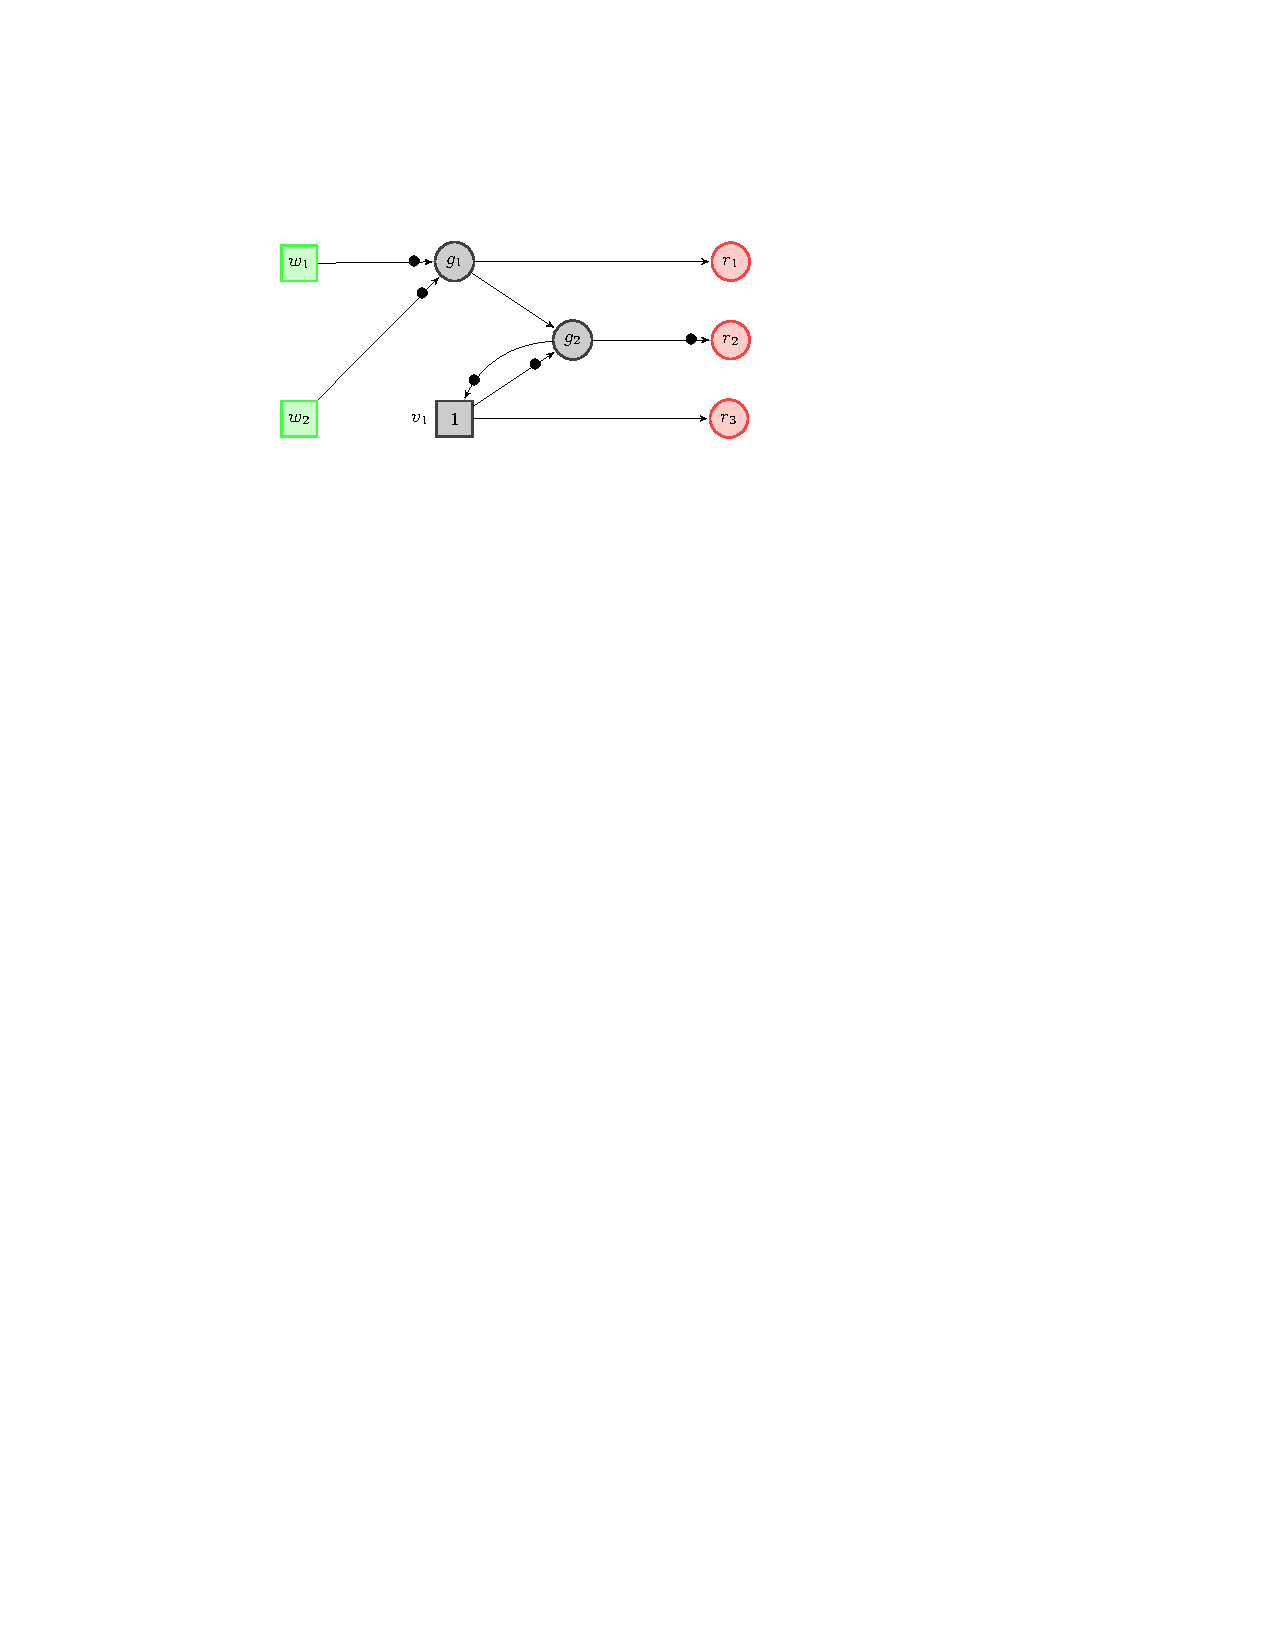
\includegraphics[width=\textwidth]{Example.pdf}
% \end{framed}
% \caption{\textbf{Left:} And-inverter graph describing a system with two
% inputs $w_1$ and $w_2$ (green boxes), one latch $v_1$ with initial value 1 (grey box), two gates $g_1$ and $g_2$ (gray circles), and three invariant requirements $r_1=\Always g_1$, $r_2=\Always \lnot g_2$ and $r_3=\Always v_1$ (red circles). 
% The arrows represent logical dependencies, and bullets in the arrows imply negation.}
% \label{fig:Preliminaries:AIGExample}
% \end{figure}
    %



\begin{figure}[!t]
	\begin{minipage}{0.6\textwidth}
	\begin{framed}
	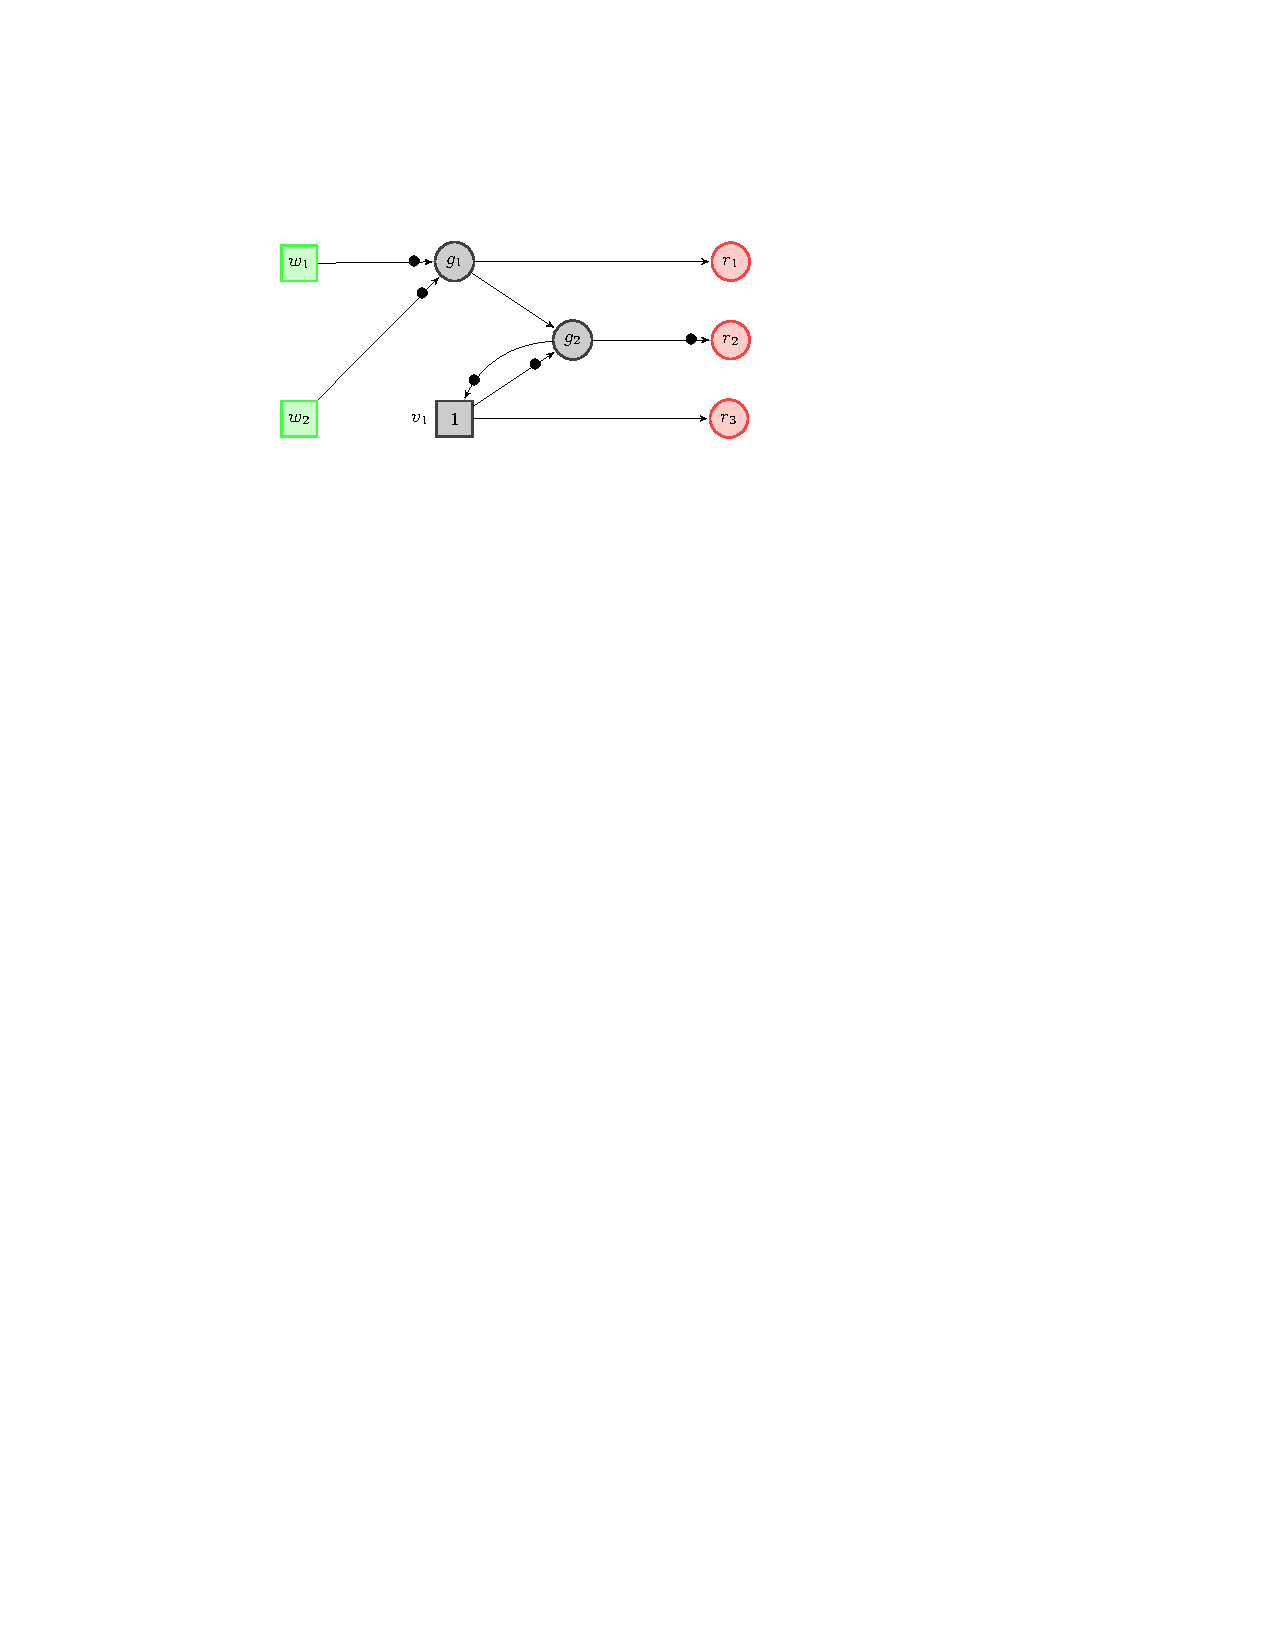
\includegraphics[width=\textwidth]{Example.pdf}
	\end{framed}
	\end{minipage}
	\begin{minipage}{0.35\textwidth}
	\centering
	\begin{framed}
	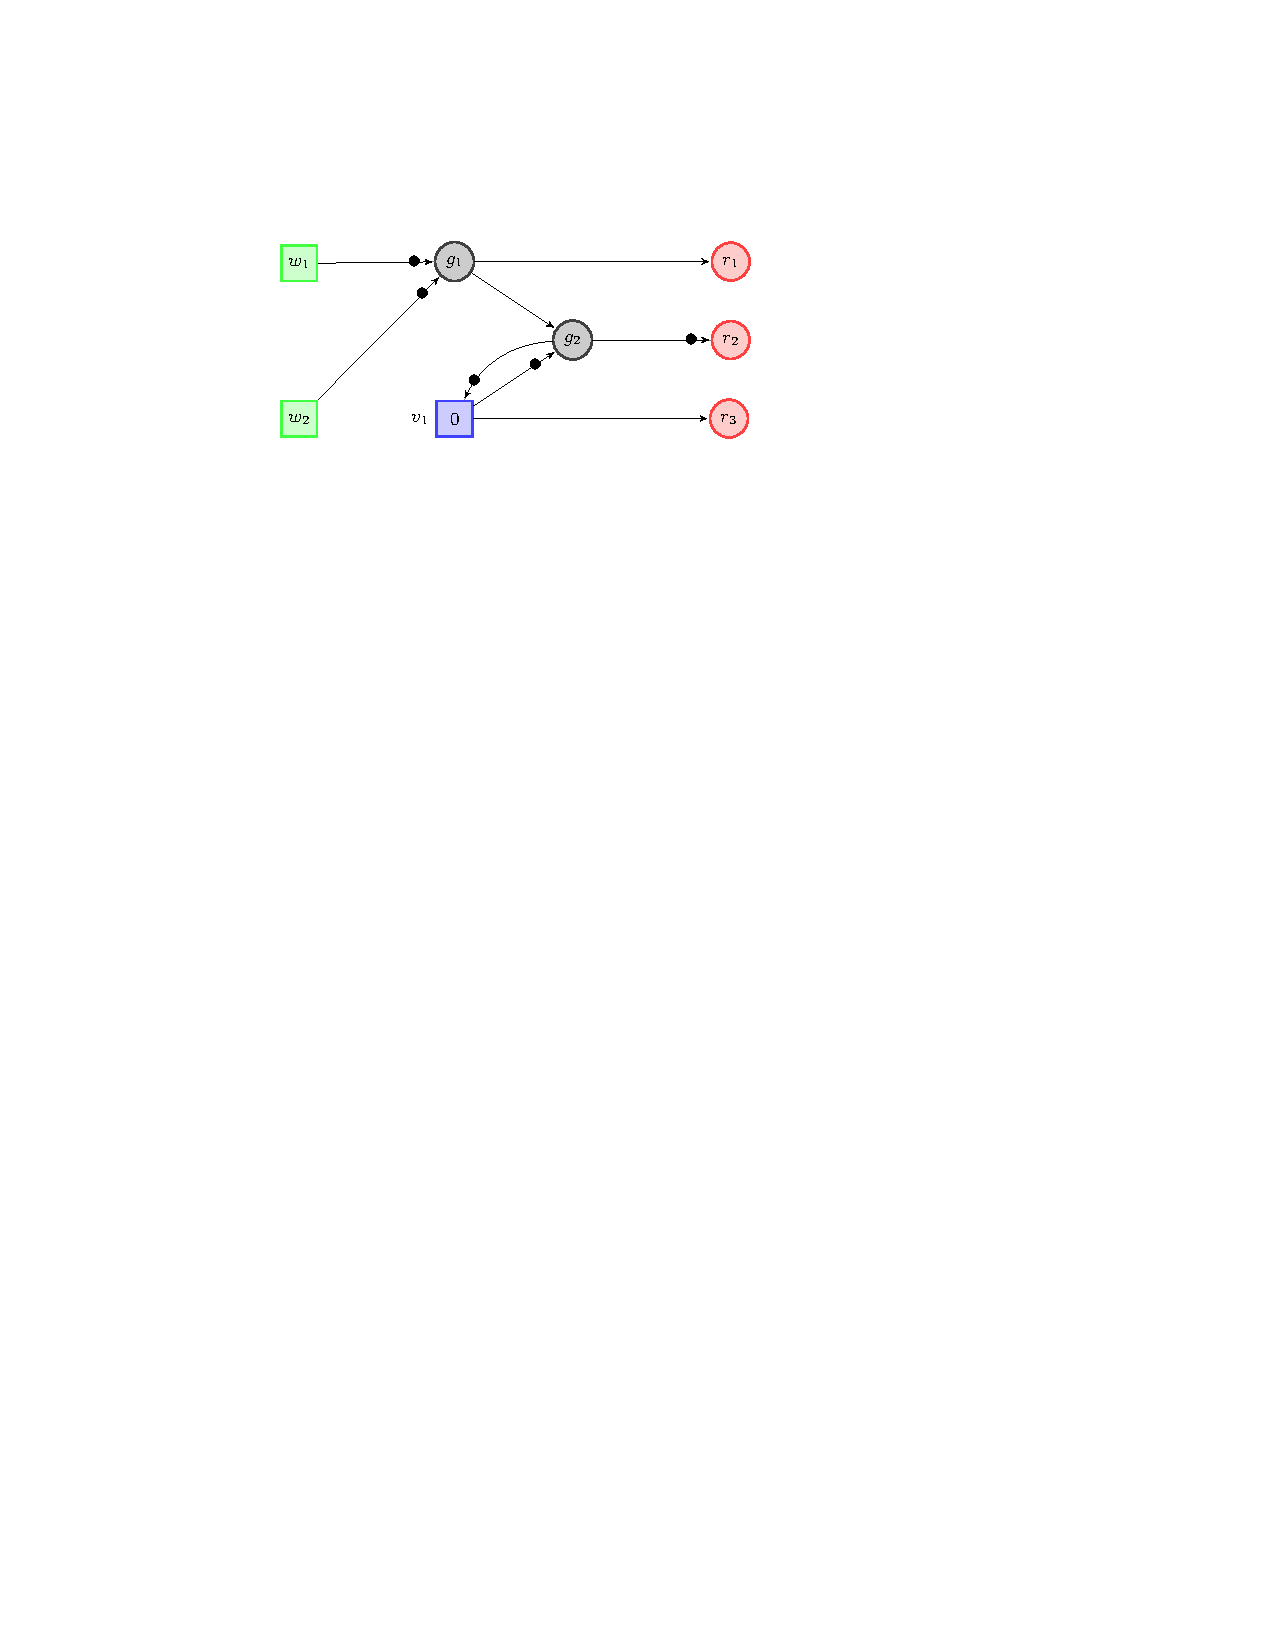
\includegraphics[width=\textwidth]{Attack2.pdf}\\
	\end{framed}
	\begin{framed}
	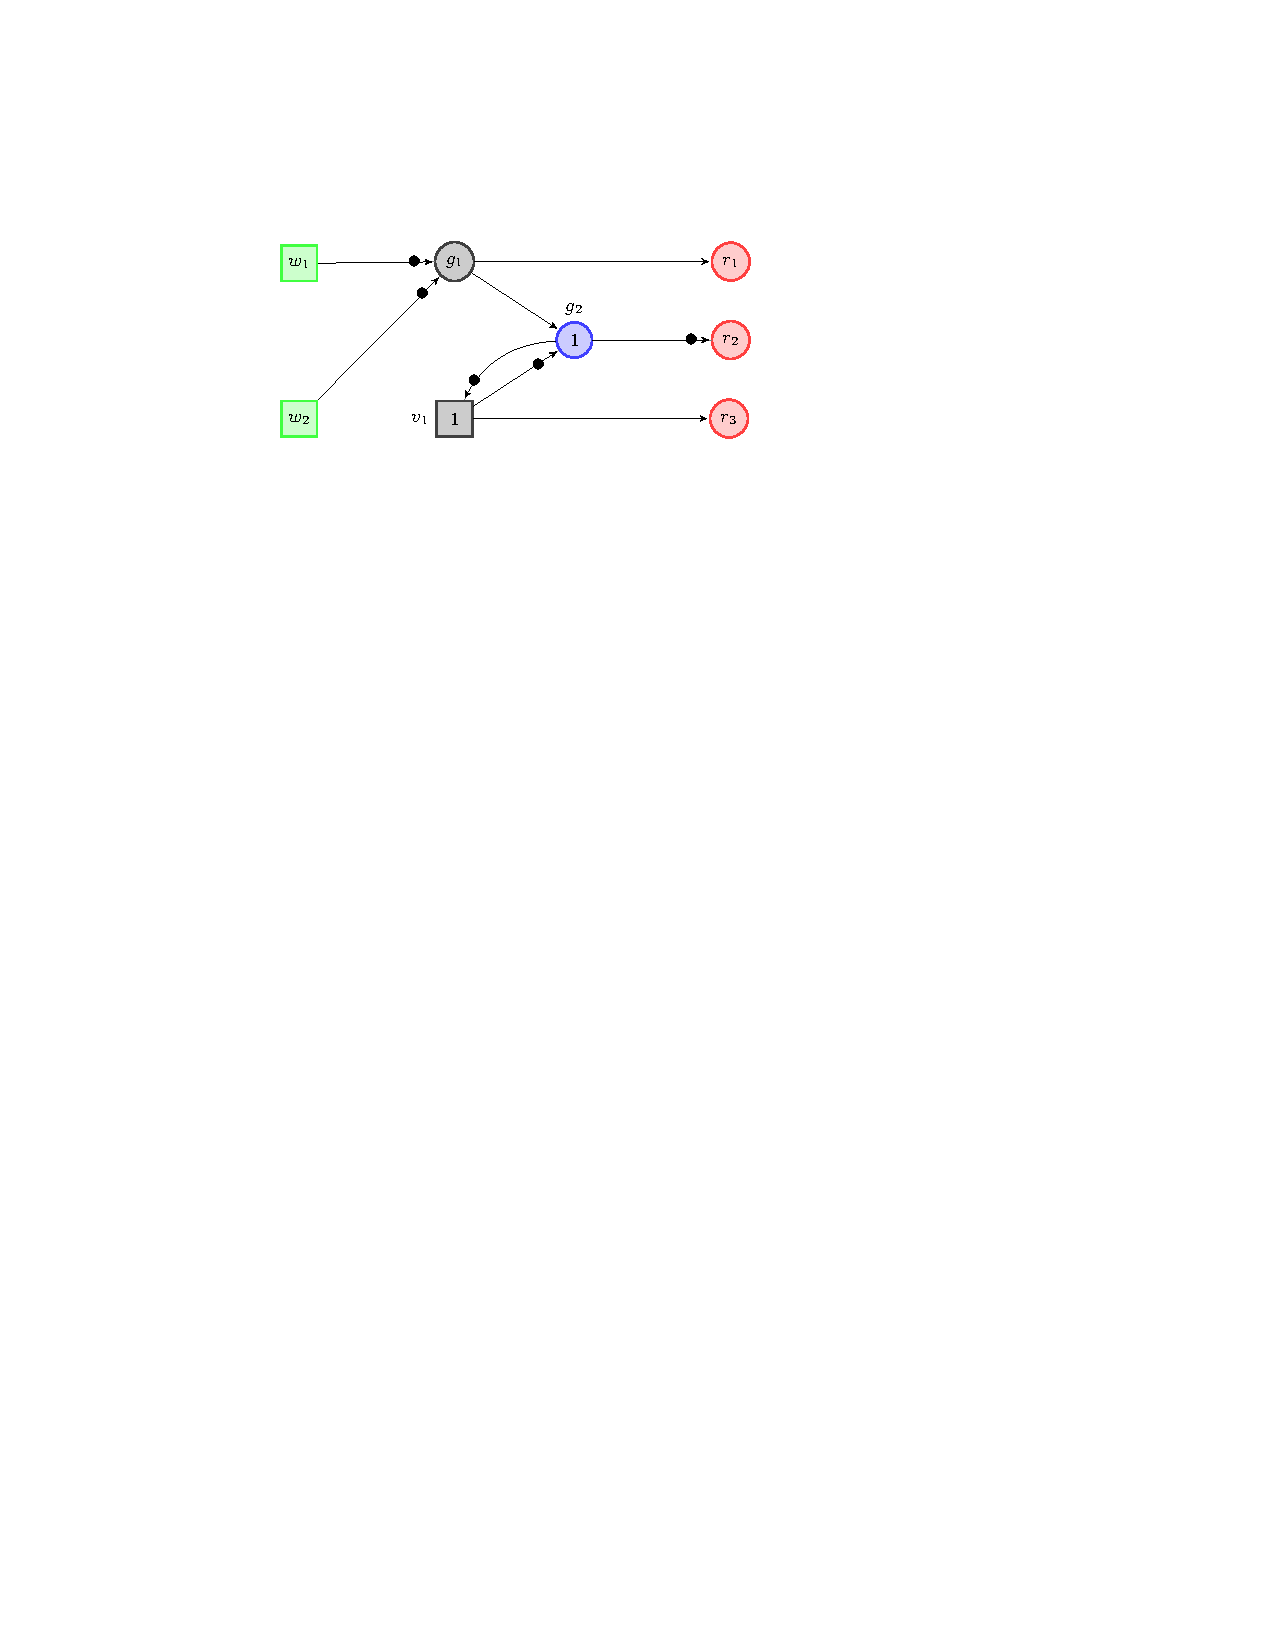
\includegraphics[width=\textwidth]{Attack1.pdf}
	\end{framed}
	\end{minipage}
	\caption{\textbf{Left:} An AIG with two
	inputs $w_1$ and $w_2$ (green boxes), one latch $v_1$ with initial value 1 (grey box), two gates $g_1$ and $g_2$ (gray circles), and three invariant requirements $r_1=\Always g_1$, $r_2=\Always \lnot g_2$ and $r_3=\Always v_1$ (red circles). 
	The arrows represent logical dependencies, and bullets in the arrows imply negation.
	\textbf{Right above}: an attacker that controls latch $v_1$ can set its initial value to 0 to break $r_2$ and $r_3$ in 0 steps. This attacker uses a spatial transformation to implement this attack.
	\textbf{Right below}: an attacker that controls gate $g_2$ can set its value to 1 at time 0 to break $r_2$ in 0 steps and $r_3$ in 1 step, because the value of $v_1$ at time 1 is 0. This attacker uses a dynamics transformation, since gates are not part of the state of AIGs.}%. An arrow with $!$ means negation}
	\label{fig:Classification:Example}
	\end{figure}

% In this section, we provide a motivational example of the problem of model checking compromised systems, and we illustrate how to classify attackers given a list of security requirements. 
 assume that an attacker $A$ controls the gate $g_2$ of the AIG shown on the left of Figure~\ref{fig:Classification:Example}. By controlling $g_2$, we mean that $A$ can choose the value of $g_2(t)$ at will for $t\geq 0$.This system fails $r_1$ at time $t$ if $w_1(t)=1$, so the attacker $A$ does not need to do anything to cause the system to fail $r_1$. Now, it is possible for $A$ to break $r_2$ at time $t=0$ and to break $r_3$ at time $t=1$ by setting $g_2(0)$ to $1$ via an attack, since $r_2=\Always \lnot g_2$, and by causing $v_1(1)$ to be equal to $0$. This attack breaks both requirements $r_2$ and $r_3$, but in general an attacker may need one attack to break one requirement, and a different attack to break another. We say that $A$ has the \emph{power to break the requirements} $r_1$, $r_2$ and $r_3$, since there are attacks in the capabilities of $A$ that break those requirements. Now, consider a different attacker $B$ which only controls the gate $g_1$. No matter what value $B$ chooses for $g_1(t)$ for all $t$, it is impossible for $B$ to break $r_2$ or $r_3$, so we say that $B$ only has the power to break $r_1$. 



If we allow attackers to control any number of coordinates, then there are $8$ different attackers, described by the subsets of $\set{v_1,g_1,g_2}$. We do not consider attackers that control inputs, because the model checking of invariant properties requires the property to hold for all inputs, so giving control of inputs to an attacker does not make it more powerful (i.e. the attacker cannot break more requirements than it already could without the inputs). Figure~\ref{fig:Classification:borders} illustrates the classification of attackers depending on whether they break a given requirement or not. Based on it, we can provide the following security guarantees: 1) the system cannot enforce $r_1$, and 2) that the system can only enforce $r_2$ and $r_3$ in the presence of attackers that are as capable to interact with the system as $\set{g_1}$ (i.e. they only control $g_1$ or nothing).

According to the classification, attacker $\set{g_2}$ is as powerful as the attacker $\set{v_1,g_1,g_2}$, since both attackers break the same requirements $r_1$, $r_2$ and $r_3$. This information may be useful to the designer of the system, because they may prioritise attackers that control less coordinates but are as powerful as attackers that control more when deploying defensive mechanisms.


\section{AIGs as $F$-coalgebras}
\label{sec:Classification:LatentBehaviours}
If we go by the strict definition of AIGs (see Section~\ref{sec:Preliminaries:AIGStates}), then only latches are part of the states of AIGs; inputs and gates are external. We, however, include gates into the state. Consider an AIG whose set of latches is $V$, its set of gates is $G$, its set of inputs is $W$ and its set of requirements is ${R}$. For each latch $v\in V$ there is an associated expression $v(t+1)$, for each gate $g\in G$, there is an associated expression $g(t)$, and each requirement $r\in {R}$ is of the form $r=\Always e$, where $e$ is an expression. 
Let $\vec{G}=2^G$, $\vec{V}=2^{V}$, $\vec{W}=2^W$ and let $\vec{{R}}=2^{{R}}$; we plan to use the set $\vec{V}\times \vec{G}$ as the carrier so that a state $(\vec{v},\vec{g})$ models the values for $\vec{v}(t+1)$ and $\vec{g}(t)$% (the values of $\vec{g}(0)$ depend on the input $\vec{w}(0)$)
. We now define the functor $F(X)=\vec{{R}}^{\vec{W}}\times X^{\vec{W}}$, and we define the $F$-coalgebra $(\vec{V}\times\vec{G},(\theta,\delta))$ where $(\theta,\delta)$ is a pair function with $\theta\colon \vec{V}\times \vec{G}\rightarrow \vec{{R}}^{\vec{W}}$, and $\delta\colon\vec{V}\times \vec{G} \rightarrow (\vec{V}\times \vec{G})^{\vec{W}}$. Given an input $\vec{w}\in \vec{W}$, the function $\delta$ maps the state $(\vec{v},\vec{g})$ to the state $(\vec{v}^{\vec{w}}, \vec{g}^{\vec{w}})$, which is defined for all $v'\in V$, $g'\in G$ and $w'\in W$, by 
\begin{align}
	\vec{v}^{\vec{w}}[v']&\triangleq \TheBehaviourOf{v'(t+1)},\\
	\vec{g}^{\vec{w}}[g']&\triangleq \TheBehaviourOf{g'(t)},
\end{align}
where $\TheBehaviourOf{g(t)}$ is the result of evaluating the expression $g'(t)$ by assuming $w'(t)=\vec{w}[w']$ and $v'(t)=\vec{v}[v']$. Note that if the expression $g'(t)$ depend on the value of $g''(t)$ where $g''$ is another gate, then we assume $g''(t)=\vec{g}^{\vec{w}}[g'']$ (AIGs are acyclic in their dependencies, only looping back to latches). Similarly, $\TheBehaviourOf{v'(t+1)}$ is the result of evaluating the expression $v(t+1)$ by assuming $w'(t)=\vec{w}[w']$, $v'(t)=\vec{v}[v']$, and $g'(t)=\vec{g}^{\vec{w}}[g']$. % instead of $g'(t)=\vec{g}[g']$. 

% for $v''\in V$, $w'\in W$ and $g''\in G$. 
The function $\theta$ evaluates the requirements given an input $\vec{w}$; for $r \in {R}$, we define
\begin{align}
	\theta(\vec{v},\vec{g})(\vec{w})[r]\triangleq \TheBehaviourOf{e(t)}, \quad \text{ if $r=\Always{e}$}, 
\end{align}
where $\TheBehaviourOf{e(t)}$ is the result of evaluating the expression $e(t)$ by assuming $w'(t)=\vec{w}[w']$, $v'(t)=\vec{v}[v']$ and $g'(t)=\vec{g}^{\vec{w}}[g']$.

%Since the set $\vec{V}\times \vec{G}$ is the carrier, 
In the following we show how to use bounded model checking to find spatial transformations which reveal a latent coalgebra that fails one or more security requirements. %whose coordinates are $V\cup G$, 
% Since the carrier is the set $\vec{V}$, spatial transformations do not directly transform the state of gates. If an attacker wants to affect a gate, they must do so via transitive data dependencies. More precisely, if a gate $g$ depends on a latch $v$ (e.g. $g(t)=v(t) \land \lnot k(t)$ where $k$ is some component, then an attacker controlling $v$ might affect $g$ by manipulating the value of the state at coordinate $v$. If the value of a gate $g$ does not transitively depend on any latch (e.g., $g_1$ in Figure~\ref{fig:Classification:Example}), then $g$ must only depend on inputs. %This follows the ideology of latent behaviour analysis, where we purposely restrict attackers to affect the state of the system.

% 



%------------------------------------------------------------------------------------------------------------------------------------------------

%-------------------------------------------------------------------------------------------------------------------------------------------------
\section{Bounded Model Checking of in the Presence of Attackers}
\label{sec:bmc}
% We recall the research questions that motivate this work: \textbf{RQ1)} given a system and a list of security requirements, how do we systematically generate attackers that can potentially break these requirements, and how do we verify if they are successful? and \textbf{RQ2)} which techniques can help us \emph{classify} attackers, i.e., to map each attacker to the set of requirements that it breaks? 
In this section, we %aim to answer these research questions on a theoretical level by 
formalise the problem of attacker model classification for AIGs using bounded model checking in the presence of attackers. More precisely, %to answer \textbf{RQ1},
we formalise attackers and their interactions with systems, and we show how to systematically generate bounded model checking problems that determine whether some given attacker breaks the security requirement being checked. We then propose two methods for the classification of attackers: 1) a brute-force method that creates a model checking problem for each attacker-requirement pair, and 2) a method that incrementally empowers attackers to find \emph{minimal attackers}, i.e. attackers which represent large portions of the universe of attackers thanks to a monotonicity relation between the set of coordinates controlled by the attacker and the set of requirements that the attacker breaks. %The latter method is a theoretical approach to answer \textbf{RQ2}, while its practical usefulness is evaluated in Section~\ref{sec:evaluation}.

\subsection{Attackers and Compromised Systems}
We modify the equations that are associated to the coordinates controlled the attacker to incorporate the possible actions of such attacker into an AIG. Formally, let $S=(W,V,G)$ be a system described by an AIG, let $R=\set{r_1, \ldots, r_n}$ be a set of invariant requirements for $S$, and let $C=V\cup G$ be the set of coordinates of $S$. An \emph{attacker model} $A$ is any subset of $C$. We refer to attackers fitting the model $A$ as \emph{$A$-attackers}. If a coordinate $c$ belongs to an attacker model $A$, then an $A$-attacker has the \emph{capability to interact with $S$ through} $c$. To capture this interaction, we modify the equations of every latch $v\in V$ to be parametrised by an attacker model $A$ as follows: the original transition equation $v(t+1)=e(t)$ and the initial equation $v(0)=b$ change to
\begin{align}
\label{eq:badLatch}
v(t+1) = \begin{cases}
e(t), \quad &\text{if $v\not \in A$;}\\
A_v(t+1), \quad &\text{otherwise},
\end{cases}
\quad 
v(0)= \begin{cases}
b, \quad &\text{if $v \not \in A$;}\\
A_v(0), \quad &\text{otherwise.}
\end{cases}
\end{align}
where $A_v(t)$ is a value chosen by an $A$-attacker at time $t$. Similarly, we modify the equation of gate $g\in G$ as follows: the original equation $g(t)=e_1(t)\land e_2(t)$ changes to
\begin{align}
\label{eq:badGate}
g(t) = \begin{cases}
e_1(t)\land e_2(t), \quad &\text{if $g\not \in A$;}\\
A_g(t), \quad &\text{otherwise},
\end{cases}
\end{align}
where $A_g(t)$ is, again, a value chosen by an $A$-attacker at time $t$. We use $A[S]$ to denote the system $S$ under the influence of an $A$-attacker; i.e., $A[S]$ is the modified system of equations. 

We now apply the definition of attacks as state transformations. An \emph{attack from an $A$-attacker}, is a function $m\colon \vec{G}\times \vec{V}\rightarrow \vec{G}\times \vec{V}$ that assigns a value to each coordinate in $A$. Given a state $\vec{x}\in \vec{G}\times \vec{V}$ and an attack $m\colon \vec{G}\times \vec{V}\rightarrow \vec{G}\times \vec{V}$, we define the \emph{ effect of $m$ on coordinates $A$ at state $\vec{x}$}, denoted $m(\vec{x})|_A\colon A\rightarrow 2$, by
\begin{align}
	m(\vec{x})|_{A}[a]\triangleq m(\vec{x})[a].
\end{align}
In the following, we consider a strategy to build an attacks for an $A$-attacker by computing the effects on coordinates $A$ in the context given by the initial state of the AIG and its successor states. Formally, we propose finding a finite sequence of vectors $\vect{a}_0,  \ldots, \vect{a}_t$ such that the vectors fix the values of all $A_c(k)$ by assuming $A_c(k)=\vect{a}_k(c)$, with $c\in A$ and $0 \leq k \leq t$. In this sense, the sequence $(\vect{a}_0, \ldots, \vect{a}_t)$ models an \emph{attack strategy to break requirements}.

% An \emph{attack strategy} is a finite sequence of attacks $(\vect{a}_0, \vect{a}_1, \ldots, \vect{a}_t)$ that fixes the values of all $A_c(k)$ (used in the equations above) by $A_c(k)=\vect{a}_k(c)$, with $c\in A$ and $0 \leq k \leq t$. %Since we have changed the semantics of the system, it is possible that $A[S]$ only satisfies a subset of requirements in $R$. 
\begin{definition}[Broken Requirement]
\label{def:brokenRequirement}
Given a requirement $r\in R$ with $r=\Always e$, we say that an $A$-attacker \emph{breaks the requirement $r$ (at time $t$)} if and only if there exists a sequence of inputs $\vec{w}_0, \ldots, \vec{w}_t$ and an attack strategy $\vect{a}_0, \ldots, \vect{a}_t$ such that $e(t)$ is false if we assume $w'(k)=\vec{w}_k[w']$ and $a'(k)=\vec{a}_k[a']$, with $0\leq k\leq t$, $w'\in W$, and $a'\in A$. We denote the set of requirements that an $A$-attacker breaks by $A[R]$. 
\end{definition}

We now define two partial orders for attackers: \textbf{1)} an $A_i$-attacker is strictly less \emph{capable} (to interact with the system) than an $A_j$-attacker in the 
context of $S$ %, denoted $A_i \leq A_j$ 
iff $A_i\subseteq A_j$ and $A_i \neq A_j$. An {$A_i$-attacker is equally capable to an $A_j$-attacker iff $A_i= A_j$}; and \textbf{2)} an $A_i$-attacker is strictly less \emph{powerful} than an $A_j$-attacker in the 
context of $S$ and $R$ %, denoted $A_i \leq A_j$ 
iff $A_i[R]\subseteq A_j[R]$ and $A_i[R]\neq A_j[R]$. Similarly, {$A_i$-attacker is equally powerful to an $A_j$-attacker iff $A_i[R]= A_j[R]$}. %We simply state that $A_i$ is less capable than $A_j$ if $S$ is clear from the context. 
% We simply say that $A_i$ is less powerful than $A_j$ if $S$ and $R$ are clear from the context.

%\subsection{Model Checking in the Presence of Attackers}
We can now properly present the problem of \emph{attacker model classification}.
\begin{definition} [Attacker Classification via Verification]
\label{def:AttackerQuantification}
Given a system $S$, a set of requirements $R$, and a set of $h$ attacker models
$\set{A_1, \ldots , A_h}$, for every attacker model $A$, we compute the set $A[R]$ of requirements that an $A$-attacker breaks by performing model checking of each requirement in $R$ on the compromised system $A[S]$. 
\end{definition}

%The duality between attackers and sets of coordinates enables the following assertions: a set of coordinates $B$ is \emph{safe} if and only if we can prove that attacker $B$ cannot break any requirements, i.e., $B[R]=\emptyset$; otherwise, the set of coordinates $B$ is  \emph{vulnerable}. 
Definition~\ref{def:AttackerQuantification} assumes that exhaustive verification is possible for $S$ and the compromised versions $A[S]$ for all attackers $A$. However, if exhaustive verification is not possible (e.g., due to time limitations or memory restrictions), we consider an alternative formulation using \emph{bounded model checking} (BMC): 
\begin{definition} [Attacker Model Classification using BMC]
\label{def:BoundedModelCheckingOfSystems}
Let $S$ be a system, $R$ be a set of requirements, and $t$ be a natural number. Given a set of attacker models $\set{A_1, \ldots , A_h}$, for each attacker model $A$ , we compute the set $A[R]$ of requirements that an $A$-attacker breaks \emph{using a strategy of length up to $t$} on the compromised system $A[S]$. 
\end{definition}
In the following, we show how to construct a SAT formula that describes the attacker model classification problem using BMC. 

\subsection{A SAT Formula for BMC up to $t$ Steps}
For a requirement $r=\Always e$ and a time step $t\geq 0$, we are interested in finding an attack strategy that causes the value of $e(k)$ to be false for some $k$ with $0\leq k \leq t$. To capture this notion, we define the proposition $\mathtt{goal}(r,t)$ by
\begin{align}
\mathtt{goal}(\Always e,t) \triangleq \bigvee_{k=0}^t{\lnot e(k)}.
\end{align}
We inform the SAT solver of the equalities and dependencies between expressions given by the definition of the AIG (e.g., that $e(k) \Leftrightarrow \lnot v_1(k)$). Inspired by the work of Biere \emph{et al.} \cite{BMCWithoutBDDs}, we transform the equations into a Conjunctive Normal Form formula (CNF) that the SAT solver can work with using  \emph{Tseitin encoding} \cite{TseitinEncoding}. Each equation of the form 
\begin{align*}
&v(0)= \begin{cases}
b, \quad &\text{if $v \not \in A$;}\\
A_v(0), \quad &\text{otherwise,}
\end{cases}
\end{align*}
becomes the formula of the form
\begin{align}
{\left(v^{\downarrow} \lor (v(0) \Leftrightarrow b ) \right)\land \left(\lnot v^{\downarrow} \lor (v(0) \Leftrightarrow A_v(0)) \right)},
\end{align}
where $v^{\downarrow}$ is a literal that marks whether the latch $v$ is an element of the attacker model $A$ currently being checked; i.e., we assume that $v^{\downarrow}$ is true if $v\in A$, and we assume that $v^{\downarrow}$ is false if $v\not \in A$. Consequently, if $v\not \in A$, then $v(0) \Leftrightarrow b$ must be true, and if $v \in A$, then $v(0)  \Leftrightarrow A_v(0) $ must be true. We denote this proposition by $\mathtt{encode}(v,0)$, and it informs the SAT solver about the initial state of the AIG.
 
Similarly, for $0\leq k<t$, each equation of the form 
\begin{align*}
&v(k+1) = \begin{cases}
e(k), \quad &\text{if $v\not \in A$;}\\
A_v(k+1), \quad &\text{otherwise},
\end{cases}\quad
\end{align*}
translates to a formula of the form
\begin{align}
&\left(v^{\downarrow} \lor (v(k+1) \Leftrightarrow e(k) ) \right)\land \left(\lnot v^{\downarrow} \lor (v(k+1) \Leftrightarrow A_v(k+1)) \right).
\end{align}
We call this formula $\mathtt{encode}(v,k)$. %We now use the Tseitin encoding of $p \Leftrightarrow (q \land r)$, i.e., $(p \lor \lnot q \lor \lnot r)\land (\lnot p \lor q)\land  (\lnot p \lor r)$, to encode gates. 

Finally, for $0\leq k \leq t$, each equation of the form
\begin{align*}
&g(k) = \begin{cases}
e_1(k)\land e_2(k), \quad &\text{if $g\not \in A$;}\\
A_g(k), \quad &\text{otherwise},
\end{cases}
\end{align*}
becomes a formula of the form
\begin{align}
&\left(g^{\downarrow} \lor (g(k) \Leftrightarrow e_1(k)\land e_2(k) ) \right)\land \left(\lnot g^{\downarrow} \lor (g(k) \Leftrightarrow A_g(k)) \right),
\end{align}
where $g^{\downarrow}$ is a literal that marks whether the gate $g$ is an element of the attacker model $A$ currently being checked in a similar way that the literal $v^\downarrow$ works for the latch $v$. We refer to this formula by $\mathtt{encode}(g,k)$.
%Consider a coordinate $c$ and an attacker $A$. Under the new system of equations, if $c\in A$, then we assume $c^{\downarrow}$ and the value of coordinate $c$ at time $k$ depends only on the literal $A_c(k)$; if $c\not\in A$, then we assume $\lnot c^{\downarrow}$ and we use the original semantics of the system to determine the value of $c$. 


Given an attacker model $A$, to perform SAT solving, we need to find an assignment of inputs in $W$ and attacker actions for each coordinate $c$ in $A$ over $t$ steps, i.e., an assignment of ${|W\times A|\times t}$ literals. The SAT problem for checking whether requirement $r$ is safe up to $t$ steps, denoted $\mathtt{check}(r,t)$, is defined by 
\begin{align}
\label{eq:naiveCheck}
\mathtt{check}(r,t)\triangleq\mathtt{goal}(r,t)\land\! \bigwedge_{c\in (V \cup G)}\left( \bigwedge_{k=0}^{t}{\mathtt{encode}(c,k)}\right).
\end{align}
If the SAT solver can provide an assignment of literals which satisfy $\mathtt{check}(r,t)$, then an $A$-attacker breaks the requirement $r$.
\begin{proposition}
\label{prop:Correctness}
For a given attacker model $A$ and a requirement $r=\Always e$, if we assume the literal $c^{\downarrow}$ for all $c \in A$ and we assume $\lnot x^{\downarrow}$ for all $x\not\in A$ (i.e., $x\in (V \cup G)-A$), then an $A$-attacker breaks the requirement $r$ in $t$ steps (or less) if and only if $\mathtt{check}(r,t)$ is satisfiable.
\end{proposition}

\begin{proof}
We first show that if an $A$-attacker breaks the requirement in $t$ steps or less, then $\mathtt{check}(r,t)$ is satisfiable. Since an $A$-attacker breaks $r=\Always e$ in $t$ steps or less, then, by Definition~\ref{def:brokenRequirement}, there exists an assignment of inputs $(\vect{w}_0, \ldots, \vect{w}_k)$ and an attacker strategy $(\vect{a}_0, \ldots, \vect{a}_k)$ which causes $e(k)$ to be false for some $k\leq t$; this means that $\mathtt{goal}(r,t)$ is satisfiable, which, in turn, makes $\mathtt{check}(r,t)$ satisfiable.

We now show that if $\mathtt{check}(r,t)$ is satisfiable, then an $A$-attacker breaks the requirement $r$ in $t$ or less steps. If $\mathtt{check}(r,t)$ is satisfiable then $\mathtt{goal}(r,t)$ is satisfiable, and $e(k)$ is false for some $k\leq t$. Consequently, there is an assignment of inputs $\vect{w}(k)$ and attacker actions $A_c(k)$, such that the $\mathtt{encode}(c,k)$ formulae are satisfied for all $c\in A$. By assuming $\vect{a}_k(c)=A_c(k)$ and $\vect{w}_k =\vect{w}(k)$, we obtain a witness input sequence and a witness attack strategy which proves that an $A$-attacker breaks $r$ in $k$ steps (i.e., in $t$ steps or less since $k\leq t$).
\end{proof}

Algorithm~\ref{alg:BadQuantification} describes a naive strategy to compute the sets $A[R]_t$ for each attacker model $A$; i.e. the set of requirements that an $A$-attacker breaks in $t$ steps (or less). Algorithm~\ref{alg:BadQuantification} works by solving, for each of the $2^{|V \cup G|}$ different attacker models, a set of $|R|$ SAT problems, 
{
each of which has a size of at least $\mathcal{O}\left({|W\cup V\cup G|\times t}\right)$ on the worst case.}

\begin{figure}[!t]
\centering
{
%\begin{framed}
\begin{algorithm}[H]
 \KwData{system $S=(W,V,G)$, a time step $t\geq 0$, a set of requirements $R$.}
 \KwResult{A map that maps the attacker $A$ to $A[R]_t$.}
Map $\mathcal{H}$\;
\For{\!\!\textbf{each} $r \in R$}
{
\For{\!\!\textbf{each} $A$ such that $A \subseteq (V\cup G)$}
	{
		\If{$\mathtt{check}(r,t)$ is satisfiable while assuming $c^\downarrow$ for all $c\in A$}
		{
			insert $r$ in $\mathcal{H}(A)$\;
		}
	 }
}
 \Return $\mathcal{H}$\;
 \caption{Naive attacker model classification algorithm.}
 \label{alg:BadQuantification}
\end{algorithm}
%\end{framed}
}
\end{figure}

We now propose two sound heuristics in an attempt to improve Algorithm~\ref{alg:BadQuantification}: the first technique aims to reduce the size of the SAT formula, while the other heuristic aims to record and propagate the results of previous verifications among the set of attacker models so that some calls to the SAT solver are avoided.

\subsection{Heuristics: Isolation and Monotonicity}
\emph{Isolation} is a strategy that uses data dependency analysis to prove that is impossible for a given attacker model to break some requirement. Informally, a requirement $r$ is isolated from an attacker model $A$ if no flow of information can occur from the coordinates in $A$ to the expression that defines $r$. To formally capture isolation, we first extend the notion of IOC to attacker models. The \emph{IOC of an attacker model $A$}, denoted $\blacktriangle(A)$, is defined by the union of IOCs of the coordinates in $A$; more precisely, 
\begin{align}
	\blacktriangle(A) \triangleq \bigcup\set{\blacktriangle(c)|c \in A}.
\end{align}
Isolation happens whenever the IOC of $A$ is disjoint from the COI of $r$, implying that $A$ cannot interact with $r$.
\begin{proposition}[Isolation]
\label{theo:isolation}
Let $A$ be an attacker model and $r$ be a requirement that is satisfied by the AIG. If $\blacktriangle(A)\cap \blacktriangledown(r)=\emptyset$, then an $A$-attacker does not break $r$.\end{proposition}
\begin{proof}

For an $A$-attacker to break the requirement $r$, there must be a coordinate $c \in \blacktriangledown(r)$ whose behaviour is affected by the presence of such $A$-attacker, causing $r$ to fail. In such a case, there must be a dependency between the variables directly controlled by the $A$-attacker and $c$, since $A$-attackers only choose actions over the coordinates they control; implying that $c\in \blacktriangle(A)$. This contradicts the premise that the IOC of $A$ and the COI of $r$ are disjoint, so the coordinate $c$ cannot exist. \qed
\end{proof}

Isolation reduces the SAT formula by dismissing attacker models that are outside the COI of the requirement to be verified. Isolation works similarly to \emph{COI reduction} (see \cite{ToSplitOrToGroup,GraphLabelingForEfficientCOIComputation,HandbookOfSatisfiability,HandbookOfModelChecking,OptimizedModelCheckingOfMultipleProperties}), and it transforms Equation \ref{eq:naiveCheck} into
\begin{align}
\label{eq:isolation}
\mathtt{check}(r,t)\triangleq\mathtt{goal}(r,t)\land\! \bigwedge_{c\in (\blacktriangledown(r)- W)}\left( \bigwedge_{k=0}^{t}{\mathtt{encode}(c,k)}\right)
\end{align}

\emph{Monotonicity} is a strategy that uses the following relation between capabilities and power of attacker models: if an attacker model $B$ has at least the same capabilities as an attacker model $A$ (i.e. $A\subseteq B$), then anything that an $A$-attacker can do, a $B$-attacker can do as well.
\begin{proposition}[Monotonicity]
\label{theo:monotonicity}
For attacker models $A$ and $B$ and a set of requirements $R$, if $A\subseteq B$, then $A[R]\subseteq B[R]$.
\end{proposition}
\begin{proof}
If $A\subseteq B$, then a $B$-attacker can always choose the same attack strategies that an $A$-attacker uses to break the requirements in $A[R]$; however, there may be strategies that a $B$-attacker uses that an $A$-attacker cannot, e.g., if $B$ has a coordinate that $A$ does not. Consequently, $A[R]\subseteq B[R]$.
\end{proof}
We use monotonicity to define a notion of {minimal (successful) attacker model} for a requirement $r$: an attacker model $A$ is a \emph{minimal attacker model} for a requirement $r$ if and only if an $A$-attacker breaks $r$, and there is no attacker model $B\subset A$ such that a $B$-attacker breaks $r$. In the following sections, we describe a methodology for attacker model classification that focuses on the identification of these minimal attacker models. %We expand on this notion in the following sections.

\subsection{Minimal (Successful) Attacker Models}
By monotonicity, any attacker model that is more capable than a minimal attacker models for a requirement $r$ breaks $r$, and any attacker model that is less capable than a minimal attacker model for $r$ cannot break $r$; otherwise, this less capable attacker model would be a minimal attacker model. In this sense, the minimal attacker models for $r$ not only partition the set of attacker models into those that break $r$ and those who do not, they create a frontier in the lattice of attacker models. For example, on the left of Figure~\ref{fig:Classification:borders}, the minimal attacker models for requirement $r_2$ are $\set{v_1}$ and $\set{g_2}$; the frontier (shown by the red arrows) is formed because any attacker model that includes them also breaks $r_2$. For these reasons, we reduce the problem of attacker model classification to the problem of finding the minimal attacker models for all requirements.

\subsubsection{Existence of a Minimal Attacker.} A requirement $r$ that is isolated from an attacker model $A$ remains safe in the presence of an $A$-attacker. Thus, for each requirement $r\in R$, if an attacker model $A$ breaks $r$, then $A$ must be a subset of ${\blacktriangledown(r)-W}$. 
Out of all the attacker models that could break $r$, the most capable attacker model is $\blacktriangledown(r)-W$. For succinctness, we henceforth denote the attacker $\blacktriangledown(r)-W$ by $r^{max}$. We check the satisfiability of $\mathtt{check}(r,t)$ with respect to the attacker model $r^{max}$ to learn whether there {exists} any other attacker model that breaks $r$ in $t$ steps; if $\mathtt{check}(r,t)$ is not satisfied, then no attacker model breaks $r$, otherwise we contradict monotonicity.

\begin{corollary}
From monotonicity and isolation (cf. Propositions \ref{theo:monotonicity} and \ref{theo:isolation}), if attacker $r^{max}$ cannot break the requirement $r$, then there are no minimal attacker models for $r$. %Equivalently, if $r^{max}$-attacker models cannot break $r$, then $r$ does not belong to any set of broken requirements $A[R]$.
\end{corollary}
\begin{figure}[!h]
\centering
{
%\begin{framed}
\begin{algorithm}[H]
 \KwData{system $S$, a requirement $r$, and a time step $t\geq 0$. }
\KwResult{set $M$ of {minimal} attacker models for $r$, bounded by $t$.}
{
\If{$check(r,t)$ is \textbf{not} satisfiable while assuming $c^\downarrow$ for all $c\in r^{max}$}
	{	
		\Return $\emptyset$\;
	}
}
Set: $P=\set{\emptyset}$, $M= \emptyset$; \quad /\!/($P$ contains the empty attacker model $\emptyset$)\\
\While{$P$ is not empty}
{
	extract $A$ from $P$ such that $A$ is minimal with respect to set inclusion\;
	\If{\textbf{not} (exists $B \in M \text{ such that } B \subseteq A)$}
	{	
        	\eIf{$\mathtt{check}(r,t)$ is satisfiable when assuming $c^\downarrow$ for all $c\in A$}
        	{
        		insert $A$ in $M$\;
        	}
        	{
        		 \For{\!\!\textbf{each} $c \in (r^{max} - A)$}
        		 {
        			insert $A \cup \set{c}$ in $P$\;
        	 	}
        
        	}
	}
	
}
\Return $M$\;

 \caption{The $\mathtt{MinimalAttackerModels}$ algorithm.}
 \label{alg:CheckRequirement}
\end{algorithm}
%\end{framed}
}
\vspace{-0.5cm}
\end{figure}

%\paragraph{Finding Minimal Attacker models.} 
After having confirmed that at least one non-isolated attacker model breaks $r$, we focus on finding minimal attacker models. Our strategy consist of starting with the smallest possible sets of capabilities (i.e. non-isolated attacker models), and systematically increasing those sets of capabilities when they fail to break the requirement $r$; we continue increasing them until they do, or we find that they are a superset of a different minimal attacker model. Algorithm~\ref{alg:CheckRequirement} describes this empowering procedure to computes the set of minimal attacker models for a requirement $r$, which we call $\mathtt{MinimalAttackerModels}$. As mentioned, we first check to see if a minimal attacker model exists (Lines 1-3); then we start evaluating attacker models in an orderly fashion by always choosing the least capable attacker model in the set of pending attacker models $P$ (Lines 5-16). Line 7 uses monotonicity to discard the attacker model $A$ if there is a known successful attacker model $B$ with $B\subseteq A$. Line 8 checks if the attacker model $A$ breaks $r$ in $t$ steps (or less); if so, then $A$ is a minimal attacker model for $r$ and is included in $M$ (Line 9); otherwise, we empower $A$ with a new coordinate $c$, and we add these new attacker models to $P$ (Lines 11-13). We note that Line 11 relies on isolation, since we only add coordinates that belong to the COI of $r$.

\begin{example}
We recall the motivational example from Section~\ref{sec:Classification:Example}. 
Consider the computation of $\mathtt{MinimalAttackerModels}$ for requirement $r_2$. In this case, $r_2^{max}$ is $\set{g1,g2,v_1}$, which breaks $r_2$. The model $r_2^{max}$ confirms the existence of a minimal non-isolated attacker model (Lines 1-3). We start to look for minimal attacker models by checking the attacker model $\emptyset$ (Lines 5-8); after we see that it fails to break $r_2$, we conclude that $\emptyset$ is not a minimal attacker model and that we need to increase its capabilities. We then derive the attacker models $\set{g_1}, \set{g_2}$ and $\set{v_1}$ by adding one non-isolated coordinate to $\emptyset$, and we put them into the set of pending attacker models (Lines 11-13). We know that the attacker models $\set{v_1}$ and $\set{g_2}$ break the requirement $r_2$, so they get added to the set of minimal attacker models, and they are not empowered (Line 9). Unlike $\set{v_1}$ and $\set{g_2}$, the attacker model $\set{g_1}$ fails to break $r_2$, so we increase its capabilities and we generate the attacker models $\set{v_1, g_1}$ and $\set{g_1, g_2}$. Finally, these two latter attacker models are supersets of minimal attacker models that we already identified, i.e., $\set{v_1}$ and $\set{g_2}$; this causes the check in Line 7 to fail, and they are dismissed from the set of pending attacker models as they are not minimal. The algorithm finishes with $M=\set{\set{v_1}, \set{g_2}}$.
\end{example}


Algorithm~\ref{alg:MinimalAttackerModels} applies Algorithm~\ref{alg:CheckRequirement} to each requirement; it collects all minimal attacker models in the set $\mathcal{M}$ and initialises the attacker model classification map $\mathcal{H}$, which maps attacker models to the sets of requirements that they break. Finally, Algorithm~\ref{alg:GoodQuantification} exploits monotonicity to compute the classification of each attacker model $A$ by aggregating the requirements broken by the minimal attacker models that are subsets of $A$.

\begin{example}
For the motivational example in Section~\ref{sec:Classification:Example}, Algorithm~\ref{alg:MinimalAttackerModels} returns $\mathcal{M}=\set{\emptyset,\set{v_1}, \set{g_2}}$ and $\mathcal{H}=\set{(\emptyset,\set{r_1}), (\set{v_1},\set{r_2, r_3}),  (\set{g_2},\set{r_2, r_3})}$. From there,  Algorithm~\ref{alg:GoodQuantification} completes the map $\mathcal{H}$, and returns
\begin{align*}
\mathcal{H}=\{&(\emptyset,\set{r_1}), (\set{v_1},\set{r_1,r_2, r_3}),  (\set{g_1},\set{r_1}),(\set{g_2},\set{r_1,r_2, r_3}), \\
&(\set{v_1,g_2},\set{r_1,r_2, r_3}),(\set{v_1,g_2},\set{r_1,r_2, r_3}),\\
&(\set{g_1,g_2},\set{r_1,r_2, r_3}),(\set{v_1,g_1,g_2},\set{r_1,r_2, r_3})\},
\end{align*}
where each pair corresponds to $(A,A[R])$ with $A$ being an attacker model and $A[R]$ being the set of requirements that $A$-attackers break.
\end{example}

\begin{figure}[!t]
%\begin{framed}
\centering
{
\begin{algorithm}[H]
 \KwData{system $S$, a time step $t\geq 0$, and a set of requirements $R$.}
 \KwResult{Set of all minimal attacker models $\mathcal{M}$ and an initial classification map $\mathcal{H}$.}
Set: $\mathcal{M}=\emptyset$\;
Map: $\mathcal{H}$\;
\For{$r \in R$}
	{
		\For{$A \in \mathtt{MinimalAttackerModels}(S,t,r)$}
		{
			insert $r$ in $\mathcal{H}(A)$\;
			insert $A$ in $\mathcal{M}$\;
		}
	 }
 \Return $(\mathcal{M},\mathcal{H})$\;
 \caption{The $\mathtt{AllMinimalAttackerModels}$ algorithm. }
 \label{alg:MinimalAttackerModels}
\end{algorithm}}
%\end{framed}
\vspace{-0.5cm}
\end{figure}


\begin{figure}[!t]
\centering
{
%\begin{framed}
\begin{algorithm}[H]
 \KwData{system $S=(W,V,G)$, a time step $t\geq 0$, a set of requirements $R$.}
 \KwResult{A map $\mathcal{H}$ that maps the attacker model $A$ to $A[R]$.}

$(\mathcal{M},\mathcal{H})=\mathtt{AllMinimalAttackerModels}(S,t,R)$\;
\For{\!\!\textbf{each} $A \subseteq {(V\cup G)}$}
{
\For{\!\!\textbf{each} $A' \in \mathcal{M}$}
	{
		\If{$A' \subseteq A$}
		{
			insert all elements of $\mathcal{H}(A')$ in $\mathcal{H}(A)$\;
		}
	 }
}
 \Return $\mathcal{H}$\;
 \caption{Improved classification algorithm. We assume that $\mathcal{H}$ initially maps every attacker model $A$ to the empty set.}
 \label{alg:GoodQuantification}
\end{algorithm}
%\end{framed}
}
\vspace{-0.5cm}
\end{figure}

\subsection{On Soundness and Completeness}
\label{sec:completeness}
Just like any bounded model checking problem, if the time parameter $t$ is below the {completeness threshold} (see \cite{EfficientComputationOfRecurrenceDiameters}), the resulting attacker model classification up to $t$ steps could be \emph{incomplete}. Informally, the completeness threshold is a time parameter which states that any bounded model checking beyond the completeness threshold never yields any new results. 
This means that an attacker model classification up to $t$ steps may prove that an attacker model $A$ cannot break some requirement $r$ with a strategy up to $t$ steps, while in reality an $A$-attacker breaks $r$ by using a strategy whose length is strictly greater than $t$. Nevertheless, there are practical reasons for using a time parameter that is lower than the completeness threshold: 1) computing the exact completeness threshold is often as hard as solving the model-checking problem \cite{HandbookOfModelChecking}, and 2) the complexity of the classification problem growths exponentially with $t$ because the size of the SAT formulae also grow with $t$; moreover, there is an exponential number of attacker models that need to be classified by making calls to the SAT solver. A classification method that uses a time bound $t$ below the completeness threshold is nevertheless \emph{sound}, i.e., the method does not falsely report that an attacker model breaks a requirement when in reality it cannot. In Section~\ref{sec:discussion} we discuss possible alternatives to overcome incompleteness and provide results with more coverage.  

Another source of incompleteness occurs when we artificially restrict minimal attacker models to a maximum size. This would be the case if we are interested in only verifying if there exists an attacker model that can break the requirements of the system by using only up to $z$ coordinates. The results of a classification whose minimal attacker models are bounded is also sound but incomplete, since does not identify minimal attacker models that have more than $z$ elements. We show in Section~\ref{sec:evaluation} that, even with restricted minimal attacker models, it is possible to obtain a high coverage of the universe of attacker models because we can extrapolate soundly those results using monotonicity.


%Given that we are already dealing with incompleteness due to time bounds, we consider the possibility of limiting the maximum size of minimal attacker models to further approximate the problem of attacker model classification. 

\subsection{Requirement Clustering}
\emph{Property clustering} \cite{ToSplitOrToGroup,HandbookOfSatisfiability,OptimizedModelCheckingOfMultipleProperties} is a state-of-the-art technique for the model checking of multiple properties. 
Clustering allows the SAT solver to reuse information when solving a similar instance of the same problem, but under different assumptions. 
To create clusters for attacker model classification, we combine the SAT problems whose COI is similar (i.e., requirements that have a Jaccard index close to one), and incrementally enable and disable properties during verification. 
More precisely, to use clustering, instead of computing $\mathtt{goal}(r,t)$ for a single requirement, we compute $\mathtt{goal}(Y,t)$ for a cluster $Y$ of requirements, defined by 
\begin{align}
%\mathtt{goal}(Y,t) \triangleq \bigwedge_{\Always e\in Y} ((\lnot r^\downarrow) \lor \bigvee_{k=0}^t{\lnot e(k)}).
\mathtt{goal}(Y,t) \triangleq \bigwedge_{r\in Y} (\lnot r^\downarrow \lor \mathtt{goal}(r,t)).
\end{align}
where $r^\downarrow$ is a new literal that plays a similar role to the ones used for gates and latches; i.e., we assume $r^\downarrow$ when we want to find the minimal attacker models for $r$, and we assume $\lnot y^\downarrow$ for all other requirements $y \in Y$. 

The SAT problem for checking whether the cluster of requirements $Y$ is safe up to $t$ steps is
\begin{align} 
\label{eq:MasterEq}
\mathtt{check}(Y,t)\triangleq\mathtt{goal}(Y,t)\land\! \bigwedge_{c\in (\blacktriangledown(Y)- W)}\left( \bigwedge_{k=0}^{t}{\mathtt{encode}(c,k)}\right),
\end{align}
where $\blacktriangledown(Y)=\bigcup \set{\blacktriangledown(r)| r\in Y}$.

%-------------------------------------------------------------------------------------------------------------------------------------------------

\section{Evaluation}
\label{sec:evaluation}
In this section, we perform experiments to evaluate the effectiveness of the isolation and monotonicity heuristics for the classification of attacker models, and we evaluate the completeness of partial classifications for different time steps. We use a sample of AIG benchmarks for evaluation; these benchmarks appeared in past Hardware Model-Checking Competitions (see \cite{HWMCC2011,HWMCC2013}) in the multiple-property verification track. Each benchmark has an associated list of invariants to be verified, which we interpret as the set of security requirements for the purposes of this evaluation. As of 2014, the benchmark set contained 230 different instances, coming from both academia and industrial settings \cite{HWMCC2014BM}. We quote from \cite{HWMCC2014BM}:
\begin{quote}
``Among industrial entries, 145 instances
belong to the SixthSense family (6s*, provided by IBM), 24 are Intel benchmarks (intel*),
and 24 are Oski benchmarks. Among the academic related benchmarks, the set includes 13
instances provided by Robert (Bob) Brayton (bob*), 4 benchmarks coming from Politecnico
di Torino (pdt*) and 15 Beem (beem*). Additionally, 5 more circuits, already present in
previous competitions, complete the set.''
\end{quote}
We run experiments on a quad core MacBook with 2.9 GHz Intel Core i7 and 16GB RAM, and we use the SAT solver CaDiCaL version 1.0.3 \cite{Cadical}. The source code of the artefact is available at \cite{aig-ac-asset}.

\paragraph{Evaluation Plan.} We separate our evaluation in two parts: 1) a comparative study where we evaluate the effectiveness of using of monotonicity and isolation for attacker model classification in several benchmarks, and 2) a case study, where we apply our classification methodology to a single benchmark --\texttt{pdtvsarmultip}-- and we study the results of varying the time parameters for partial classification.

\subsection{Evaluating Monotonicity and Isolation}
Given a set of competing classification methodologies $\mathcal{M}_1,\ldots, \mathcal{M}_n$ (e.g., Algorithm~\ref{alg:BadQuantification} and Algorithm~\ref{alg:GoodQuantification}), each methodology is given the same set of benchmarks $S_1,\ldots, S_m$, each with its respective set of requirements $r_1, \ldots, r_m$. To evaluate a methodology $\mathcal{M}$ on a benchmark $S=(W,V,G)$ with a set of requirements $R$, we allow $\mathcal{M}$ to ``learn'' for about 10 minutes per requirement by making calls to the SAT solver, and produce a (partial) attacker model classification $\mathcal{H}$.  Afterwards, we compute the \emph{coverage} of $\mathcal{M}$.

\begin{definition}[Coverage]
Let $\ThePowersetOf{C}$ be the set of all attacker models, and let $\mathcal{H}$ be the attacker model classification produced by the methodology $\mathcal{M}$. The relation $\mathcal{H}$ maps each attacker model $A$ to a set of requirements that an $A$-attacker breaks, with $\mathcal{H}(A)\subseteq A[R]$, for each attacker $A$ (the classification is sound and complete iff $\mathcal{H}(A)= A[R]$). The \emph{attacker model coverage obtained by methodology $\mathcal{M}$ for a requirement $r$} is the percentage of attacker models $A\in\ThePowersetOf{C}$ for which we can correctly determine whether $A$-attackers break $r$ only by computing $r\in \mathcal{H}(A)$ (i.e.,do not allow guessing and we do not allow making new calls to the SAT solver).
\end{definition}

We measure the execution time of the classification per requirement; i.e., the time it takes for the methodology to find minimal attacker models, capped at about 10 minutes per requirement. We force stop the classification for each requirement if a timeout occurs, but not while the SAT solver is running (i.e., we do not interrupt the SAT solver), which is why the reported time sometimes  exceeds 10 minutes.

\subsection{Effectiveness of Isolation and Monotonicity}
To test the effectiveness of isolation and monotonicity, we select a small sample of seven benchmarks. For each benchmark, we test four variations of our methodology: 
\begin{enumerate}
\item{$(+IS, +MO)$}: Algorithm~\ref{alg:GoodQuantification}, which uses both isolation and monotonicity
\item{$(+IS,-MO)$}: Algorithm~\ref{alg:GoodQuantification} but removing the check for monotonicity on Algorithm~\ref{alg:CheckRequirement}, Line 7;
\item{$(-IS,+MO)$}: Algorithm~\ref{alg:GoodQuantification} but using Equation~\ref{eq:isolation} instead of Equation~\ref{eq:MasterEq} to remove isolation while preserving monotonicity; and 
\item{$(+IS,+MO)$} Algorithm~\ref{alg:BadQuantification}, which does not use isolation nor monotonicity. 
\end{enumerate}

\paragraph{Setup.}{The benchmarks we selected have an average of 173 inputs, 8306 gates, 517 latches, and 80 requirements. } We arbitrarily define the time step parameter $t$ to be ten. Now, following our formulation of attacker models, which uses $V\cup G$ as the set of coordinates, we observe that these benchmarks have on average $2^{8823}$ attacker models. %, compared to 80 properties to be checked in model checking competitions
% . 
However, since an attacker that controls a gate $g$ can be emulated by an attacker that controls all latches in the sources of $g$, we choose to restrict attacker models to be comprised of only latches; i.e. the set of coordinates used by attacker models is now $V$. This restriction reduces the size of the set of attacker models from $2^{8823}$ to $2^{517}$ on average per benchmark. 

We arbitrarily restrict the number of coordinates that minimal attacker models may control to a maximum of three. This restriction represents the arbitrary decision of accepting the risk of not defending against attackers controlling more than four gates (possibly due to the improbability of those attackers gaining control over those components in the first place). This decision implies that we would need to make at most $80\times\sum_{k=0}^3 \binom {517}k$ calls to the SAT solver per benchmark. 

\paragraph{Results.} Figure~\ref{fig:Classification:AverageCoverage} illustrates the average coverage for the four different methodologies, for each of the seven benchmarks. The exact coverage values are reported in Tables~\ref{tab:Classification:AllResults1} and \ref{tab:Classification:AllResults2}. We see that the methodology which uses isolation and monotonicity consistently obtains the best coverage of all the other methodologies, with the exception of benchmark $\mathtt{6s155}$, where the methodology that removes isolation performs better. We attribute this exception to the way the SAT solver reuses knowledge when working incrementally; it seems that, for $(-IS,+MO)$, the SAT solver can reuse more knowledge than for $(+IS,+MO)$, which is why $(-IS,+MO)$ can discover more minimal attacker models in average than $(+IS,+MO)$. 

We observe that the most significant element in play to obtain a high coverage is the use of monotonicity. Methodologies that use monotonicity always obtain better results than their counterparts without monotonicity. Isolation does not show a trend for increasing coverage, but has an impact in terms of classification time. Figure~\ref{fig:Classification:AverageExecTime} presents the average classification time per requirement for the benchmarks under the different methodologies. We note that removing isolation often increases the average classification time of classification methodologies; the only exception --benchmark $\mathtt{6s325}$-- reports a smaller time because the SAT solver ran out of memory during SAT solving about $50\%$ of the time, which caused an early termination of the classification procedure. This early termination also reflects on the comparatively low coverage for the method $(-IS,+MO)$ in this benchmark, reported on Figure~\ref{fig:Classification:AverageCoverage}.

\begin{figure}[!t]
%\begin{minipage}{0.25\textwidth}
\centering
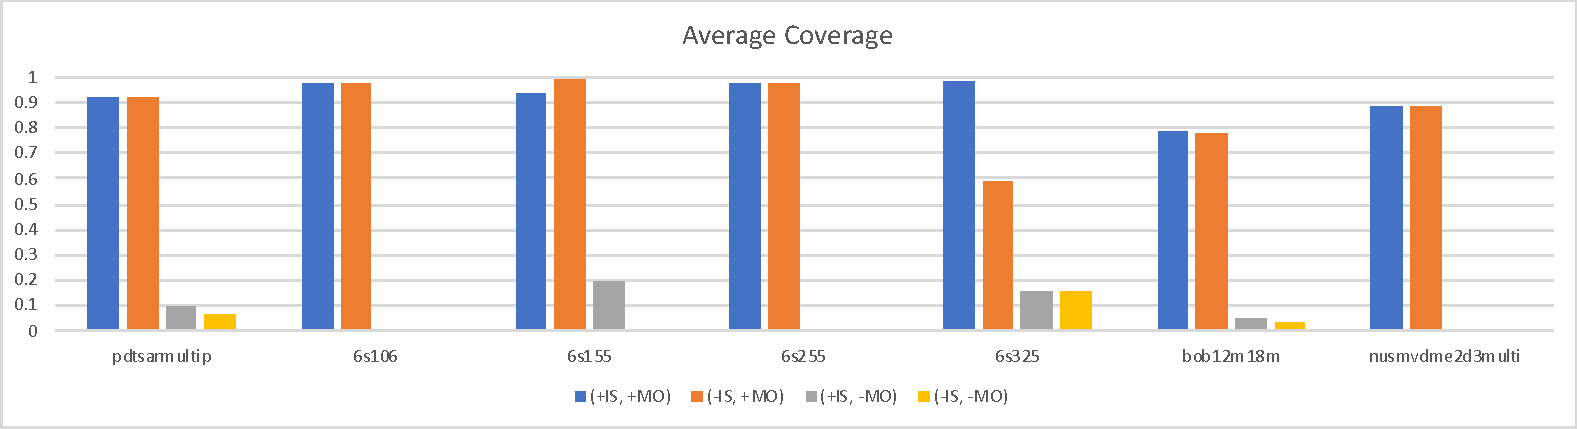
\includegraphics[width=\textwidth]{AverageCoverage}
\caption{Average requirement coverage per benchmark. A missing bar indicates a value that is approximately 0.}
\label{fig:Classification:AverageCoverage}
\vspace{0.5cm}
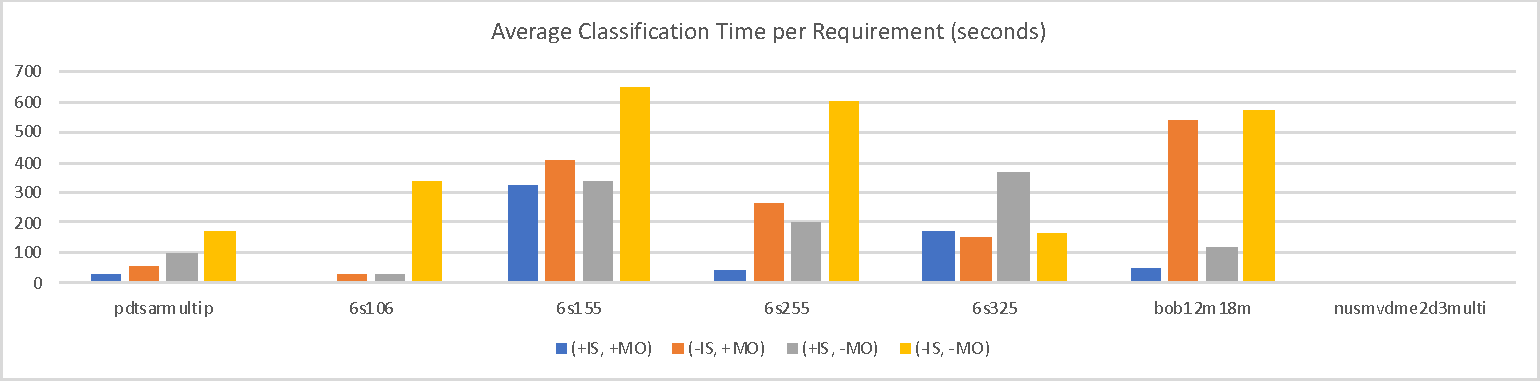
\includegraphics[width=\textwidth]{AverageExecutionTime}
\caption{Average classification time per requirement per benchmark. A missing bar indicates a value that is approximately 0. }
\label{fig:Classification:AverageExecTime}
%\end{minipage}
\end{figure}


\subsection{Partial Classification of the \texttt{pdtvsarmultip} Benchmark}
The benchmark \texttt{pdtvsarmultip} has 17 inputs, %giving values to the variables $v_{1}$ to $v_{17}$; it has 
130 latches, %ranging from $v_{18}$ to $v_{147}$; it has 
2743 gates, %ranging from $v_{148}$ to $v_{2743}$; 
and has an associated list of 33 invariant properties, out of which 31 are different (three requirements are equal). We interpret those 31 invariants as the list of security requirements. 
Since we are only considering attacker models that control latches, there are a total of $2^{130}$ attacker models that need to be classified for the 31 security requirements.
% {\color{red}

We consider six scenarios for the partial classification up to $t$ steps. We allow $t$ to take values in the set $\set{0,1,5,10,20,30}$. We obtain the execution time of classification (ms), the size of the set of source latches for the requirement (\#C), the number of minimal attacker models found (\#Min.), the total number of calls to the SAT solver (\#SAT), the average number of coordinates per minimal attacker (\#C./Min) and the coverage for the requirement (Cov.) for each requirement. We present the average of these measures in Table~\ref{tab:pdt}. 

Normally, the attacker model classification behaves in a similar way to what is reported for requirement $ \Always \lnot g_{2177}$, shown in Table~\ref{tab:pdt2324}. More precisely, coverage steadily increases and stabilises as we increase $t$. However, we like to highlight two interesting phenomena that may occur: 1) coverage {may} \emph{decrease} as we increase the time step (e.g., as shown in Table~\ref{tab:pdt2367}), and 2) the number of minimal attacker models decreases while the coverage increases, as in Tables~\ref{tab:pdt2324} and ~\ref{tab:pdt2367}. 

The coverage may decrease as we increase the time step occurs because the set of attacker models whose actions affect requirements at time 0 is rather small, i.e., $2^6$, because the effect of actions by other attackers do not have time to propagate. When we consider one step of propagation, the set of attacker models whose actions affect the requirements at times 0 and 1 has size $2^{26}$. The size of this set increases with time until it stabilises at $2^{66}$, which is the size of the set of attackers that cannot be dismissed by isolation. 

The number of minimal attacker models may decrease as the coverage increases because the minimal attacker models that are found for smaller time steps may require more components on average to break requirements than the minimal attacker models that are found when we give more time for effect of attacks to propagate. 
%represent a small percentage of the set of attackers that can affect the system, so there is very little we can learn by using monotonicity. 
More precisely, those minimal attacker models control a relatively large set of coordinates, which they need to be successful in breaking requirements, as shown in Step 5, column \#C./Min in Tables~\ref{tab:pdt2324} and~\ref{tab:pdt2367}. By considering more time steps, we are allowing attackers that control less coordinates to further propagate their actions through the system, which enables attack strategies that were unsuccessful for smaller choices of time steps.

\begin{table}[!t]
\centering
\caption{Average measures for all requirements per time steps.}
{
	%\small
\begin{tabular}{|c|c|c|c|c|c|c|}
\hline
Steps & ms &  \#C. & \#Min. & \#SAT & \#C./Min. & Cov.\\
\hline
0 & 683.12903 & 34.967741 & 2.4516129 & 16328.774 & 1.4 & 0.5272775\\
1 & 2387.5483 & 46.225806 & 6.3870967 & 24420 & 1.6502324 & 0.5725332\\
5 & 5229.9354 & 58.935483 & 44.903225 & 28355.290 & 1.6396456 & 0.849569\\
10 & 24967.129 & 58.935483 & 151.19354 & 25566.548 & 1.4608692 & 0.9189732\\
20 & 13632.516 & 58.935483 & 17.677419 & 20849.709 & 1.1762725 & 0.9793542\\
30 & 12208.258 & 58.935483 & 15.935483 & 20798.161 & 1.1045638 & 0.9793542\\
\hline
\end{tabular}}
\label{tab:pdt}
\end{table}
\begin{table}[!t]
\centering
%\begin{minipage}{0.65\textwidth}
%\begin{minipage}{0.45\textwidth}
\caption{Coverage for $\Always \lnot g_{2177}$.}
%\resizebox{\textwidth}{!}
{
\begin{tabular}{|c|c|c|c|c|c|c|}
\hline
\multicolumn{7}{|c|}{$\Always \lnot g_{2177}$} \\
\hline
Steps & ms & \#C & \#Min. & \#SAT & \#C./Min. & Cov.\\
\hline
0 & 895 & 59 & 0 & 34281 & -- & 5.94E-14\\
1 & 2187 & 66 & 10 & 47378 & 2 & 0.499511\\
5 & 1735 & 66 & 205 & 12476 & 1.912195 & 0.999997\\
10 & 968 & 66 & 27 & 9948 & 1 & 0.999999\\
20 & 1275 & 66 & 27 & 9948 & 1 & 0.999999\\
30 & 1819 & 66 & 27 & 9948 & 1 & 0.999999\\
 \hline
\end{tabular}
}
\label{tab:pdt2324}
\end{table}

% \end{minipage}
% \vspace{1cm}
% \begin{minipage}{0.45\textwidth}
\begin{table}[!t]
	\centering
\caption{Coverage for $\Always \lnot g_{2220}$.}
%\resizebox{\textwidth}{!}
{
\begin{tabular}{|c|c|c|c|c|c|c|}
\hline
\multicolumn{7}{|c|}{$\Always \lnot g_{2220}$} \\
\hline
Steps & ms &  \#C. & \#Min. & \#SAT & \#C./Min. & Cov.\\
\hline
0 & 1 & 6 & 1 & 28 & 1 & 0.90625\\
1 & 86 & 26 & 1 & 2628 & 1 & 0.500039\\
5 & 4511 & 67 & 17 & 47664 & 2.588235 & 0.852539\\
10 & 3226 & 67 & 6 & 37889 & 1 & 0.984375\\
20 & 3355 & 67 & 6 & 37889 & 1 & 0.984375\\
30 & 3562 & 67 & 6 & 37889 & 1 & 0.984375\\
 \hline
\end{tabular}
}
\label{tab:pdt2367}
% \end{minipage}
\end{table}


By taking an average over all requirements, we observe that coverage seems to steadily increase as we increase the number of steps for the classification, as reported in Table~\ref{tab:pdt}, column Cov. The low coverage for small $t$ is due to the restriction on the size of minimal attacker models; if we allowed more coordinates for minimal attackers, then the effect of their attacks may propagate faster to the target requirements. More precisely, for small $t$, attackers can only use short strategies, which limits their interaction with the system. In this sense, we expect minimal attacker models to control a large number of coordinates if they want to successfully influence a requirement in a single time step, and since we restricted our search to attacker models of maximum size three, those larger attacker models remain unexplored (e.g., as reported in Table~\ref{tab:pdt2324} for Step 0).

We conclude that experimental evidence favours the use of both monotonicity and isolation for the classification of attacker models, although some exceptions may occur for the use of isolation. In general, monotonicity and isolation help the classification methodology $(+IS,+MO)$ consistently obtain significantly better coverage compared to the naive methodology $(-IS,-MO)$.
%-------------------------------------------------------------------------------------------------------------------------------------------------

\section{Related Work}
\label{sec:discussion}
\paragraph{On Defining Attackers.} Describing an adequate attacker model to contextualise the security guarantees of a system is not a trivial task. Some attacker models may be adequate to provide guarantees over one property, but not for a different one (e.g., the Dolev-Yao attacker model is sensible for confidentiality properties, but not so much for integrity properties). Additionally, depending on the nature of the system and the security properties being studied, it is sensible to describe attackers at different levels of abstraction. For instance, in the case of security protocols, Basin and Cremers define attackers in~\cite{KnowYourEnemy} as combinations of compromise rules that span over three dimensions:  \emph{whose} data is compromised, \emph{which} kind of data it is, and \emph{when} the compromise occurs. In the case of Cyber-physical Systems (CPS), works like \cite{Giraldo2018} model attackers as sets of components (e.g., some sensors or  actuators), while other works like \cite{IFCPSSec,Cardenas2011,Urbina2016} model attackers that can arbitrarily manipulate any control inputs and any sensor measurements at will, as long as they avoid detection. In the same context of CPS, Rocchetto and Tippenhauer \cite{CPSProfiles} model attackers more abstractly as combinations of quantifiable traits (e.g., insider knowledge, access to tools, and financial support); these traits, when provided a compatible system model, ideally fully define how the attacker can interact with the system. 


Our methodology for the definition of attackers combines aspects from~\cite{KnowYourEnemy} and \cite{Giraldo2018}. The authors of~\cite{KnowYourEnemy} define symbolic attackers and a set of rules that describe how the attackers affect the system, which is sensible since many cryptographic protocols are described symbolically. Our methodology describes attackers as sets of coordinates (staying closer to the definitions of attackers in \cite{Giraldo2018}), and has a lower level of abstraction since we describe the semantics of attacker actions in terms of how they change the functional behaviour of the AIG, and not in terms of what they ultimately represent. This lower level of abstraction lets us systematically and exhaustively generate attacker models for a given system by using the definition of such system, but those models do not automatically translate to other systems. Basin and Cremers compare the effect of attackers across different protocol implementations because their attacker models have the same abstract semantics. If we had an abstraction function from sets of gates and latches to abstract effects (e.g., ``gates in charge of encryption'', or ``latches in charge of redundancy''), then it could be possible to compare results amongst different AIGs.

In Chapter~\ref{ch:CPSRobustness}, we expand the notion of attacker models that we used in this chapter, i.e., attacker models as sets of coordinates, by adding a new component: \emph{attack preconditions}. If coordinates determine \emph{which} components are compromised and \emph{how}, then attack preconditions define \emph{when} they are compromised.

\paragraph{On Efficient Classification.} 
The works by Cabodi, Camurati and Quer \cite{GraphLabelingForEfficientCOIComputation}, Cabodi et. al \cite{ToSplitOrToGroup}, and Cabodi and Nocco \cite{OptimizedModelCheckingOfMultipleProperties} present several useful techniques that may improve the performance of model checking when verifying multiple properties, including COI reduction and property clustering. We also mention the work by Goldberg et al. \cite{JustAssume} where they consider the problem of efficiently checking a set of safety properties $P_1$ to $P_k$ by individually checking each property while assuming that all other properties are valid. These works inspired us to incrementally check requirements in the same cluster, helping us transform Equation~\ref{eq:naiveCheck} into Equation~\ref{eq:MasterEq}. Nevertheless, we note that all these techniques are described for model checking systems in the absence of attackers, which is why we needed to introduce the notions of isolation and monotonicity to account for them. We believe that it may be possible to use or incorporate other techniques that improve the efficiency of BMC in general (e.g., interpolation \cite{Interpolation}), but such optimisations are beyond the scope of this work.

\paragraph{On Completeness.} As mentioned in Section~\ref{sec:completeness}, if the time parameter for the classification is below the {completeness threshold}, the resulting attacker model classification is most likely {incomplete}. To guarantee completeness, it may be possible to adapt existing termination methods (e.g. \cite{ProvingMorePropertiesWithBMC}) to incorporate attacker models. Alternatively, methods that compute a good approximation of the completeness threshold (e.g. \cite{EfficientComputationOfRecurrenceDiameters}) should not only improve coverage in general but also the reliability of the resulting attacker model classifications.  Interpolation \cite{Interpolation} could also help finding a guarantee of completeness. 

Finally, if we consider alternative verification techniques to BMC, then IC3 \cite{IC3,IC32} and PDR \cite{IC3}, which have seen some success in hardware model checking, may address the limitation of boundedness.

\paragraph{On Verifying Non-Safety Properties.} In this work, we focused our analysis exclusively on safety properties of the form $\Always e$. However, it is possible to extend this methodology to other types of properties, as it is possible to efficiently encode Linear Temporal Logic formulae for bounded model checking \cite{BMCWithoutBDDs,lmcs:2236}. The formulations of the SAT problem change for the different formulae, but both isolation and monotonicity should remain valid heuristics; ultimately, monotonicity and isolation are about the sound extrapolation of the validity of attack strategies among attacker models that have related capabilities.

\section{Summary}
\label{sec:Classification:Summary}
\todo[inline]{TLDR of this chapter. We apply LBA to very restricted systems and we obtain ordering of attackers, which is an interesting thing to use when we want to find which attacker is the most pressing. Next chapter we show how to repair those attacks. }
In this chapter we model AIGs as $F$-coalgebras, and we model their attackers as sets of spatial transformations. We use bounded model checking to classify and compare attackers, which provides an answer for Research Question~\ref{que:Classification} in the case of AIGs. Due to the exponential size of the problem, we propose a set of heuristics to perform bounded model efficiently, for which we provide experimental evidence.

The contents of this chapter are published in ~\cite{ClassificationOfAttackers}.
%-------------------------------------------------------------------------------------------------------------------------------------------------
\section{Conclusion}
\label{sec:Classification:conclusion}
% In this chapter, we presented a methodology to model check systems in the presence of attackers with the objective of mapping each attacker model to the set of security requirements broken by attackers that fit the model. This mapping of attacker models creates a classification for them, defining equivalence classes of attacker models by both set inclusion and by the set of requirements broken by their attackers. While it is possible to perform a classification of attackers by exhaustively performing model checking, the exponential size of the set of attackers renders a naive approach impractical. Thus, we rely on ordering relations between attackers to efficiently classify a large percentage of them. We provide empirical evidence by applying our methodology to a set of AIG benchmarks, which describe hardware systems at a bit level.
It surprised us that finding minimal attacker models that had only one coordinate was relatively simple. Informally, this means that the systems we studied were not robust: all it takes is for one single component to fail or be attacked, and the systems start to fail their security requirements. Since altering a single component already causes systems to fail, we conclude that using SAT solvers and BMC might have been a bit excessive for the purposes of attacker classification; it could have sufficed to systematically test the systems instead of checking them. In Chapter~\ref{ch:CPSRobustness}, we switch from a verification to a testing methodology.

% and they can give us attacks, but that maybe we need not verify a system: we should test them instead, since we expect them to fail when in the presence of attackers. This takes us to the second application on CPSs

% A system is considered safe in the presence of attackers if no attacker model breaks any requirement. However, In our view, ensuring the completeness of the attacker model classification is the most relevant direction for future work. Unlike complete classifications, incomplete classifications cannot provide guarantees that work in the general case if minimal attackers are not found. We also note that the effectiveness of monotonicity for classification is directly related to finding minimal attackers. Consequently, our methodology may benefit from any other method that helps in the identification of those minimal attackers. In particular, we are interested in checking the effectiveness of an approach where, instead of empowering attackers, we try to {reduce} successful attackers into minimal attackers by removing unnecessary capabilities. This, formally, is an \emph{actual causality analysis} \cite{ActualCausality} of successful attackers.

%-------------------------------------------------------------------------------------------------------------------------------------------------

\newpage
\begin{landscape}
	\begin{table}[!t]
		\centering		
		\centering
		\begin{tabular}{|c|c|c|c|c|c|c|c|}
			\hline
			Benchmark  & pdtsarmultip & 6s106       & 6s155       & 6s255       & 6s325       & bob12m18m   & nusmvdme2d3multi \\ \hline
			\multicolumn{8}{|c|}{Average Coverage per Requirement}                                                             \\ \hline
			(+IS, +MO) & 0.918973269  & 0.977620187 & 0.93762207  & 0.977172852 & 0.986949581 & 0.785075777 & 0.8853302        \\
			(-IS, +MO) & 0.916622423  & 0.977008259 & 0.99609375  & 0.9765625   & 0.590205544 & 0.781704492 & 0.8853302        \\
			(+IS, -MO) & 9.95E-02     & 2.01E-03    & 0.1953125   & 1.73828E-11 & 0.156147674 & 4.61E-02    & 4.52E-15         \\
			(-IS, -MO) & 6.45E-02     & 9.10E-36    & 6.00E-72    & 2.0838E-222 & 0.156146179 & 3.29E-02    & 4.52E-15         \\ \hline
			\multicolumn{8}{|c|}{Average Classification Time per Requirement}                                                  \\ \hline
			(+IS, +MO) & 24967.12903  & 3088.882353 & 326372.2188 & 38396.125   & 174066.6047 & 49916.59211 & 3530.666667      \\
			(-IS, +MO) & 56187.48387  & 25090.47059 & 408165.4063 & 263457.125  & 152425.3889 & 541870.25   & 3348.333333      \\
			(+IS, -MO) & 97326.29032  & 28483.11765 & 340715.0313 & 197275.75   & 363913.8472 & 114330.0855 & 3890             \\
			(-IS, -MO) & 170630.7742  & 341430.7059 & 646926.0625 & 602012.5    & 162959.5436 & 572080.0987 & 4262.333333      \\ \hline
			\multicolumn{8}{|c|}{Average Number of Components to Build Attackers From per Requirement}                         \\ 
			\hline
			(+IS, +MO) & 58.93548387  & 35.47058824 & 9           & 93.875      & 173.1196013 & 124.0460526 & 63               \\
			(-IS, +MO) & 82           & 135         & 257         & 752         & 1668        & 261         & 63               \\
			(+IS, -MO) & 58.93548387  & 35.47058824 & 9           & 93.875      & 173.1196013 & 124.0460526 & 63               \\
			(-IS, -MO) & 82           & 135         & 257         & 752         & 1668        & 261         & 63               \\ 
			\hline
			% \multicolumn{8}{|c|}{Average Number of Identified Successful Attackers per Requirement}                            \\ \hline
			% (+IS, +MO) & 151.1935484  & 16.05882353 & 7.5         & 2.5625      & 237.3056478 & 34.93421053 & 129.3333333      \\
			% (-IS, +MO) & 146.0322581  & 16.05882353 & 8           & 2.4375      & 46.42424242 & 34.68421053 & 129.3333333      \\
			% (+IS, -MO) & 15860.25806  & 14693.17647 & 98          & 13792.9375  & 214293.01   & 22700.58553 & 1282             \\
			% (-IS, -MO) & 27207.54839  & 105842.7059 & 126133.2813 & 20657       & 2502.25641  & 40526.72368 & 1282             \\ 
			% \hline
			% \multicolumn{8}{|c|}{Average Number of Calls to SAT Solver per Requirement}                                        \\ \hline
			% (+IS, +MO) & 25566.54839  & 1978.647059 & 10.4375     & 11382.125   & 583123.7209 & 300825.9605 & 40576.33333      \\
			% (-IS, +MO) & 58420.83871  & 294477.9412 & 2022640.25  & 35252.1875  & 51411.24747 & 1607803.138 & 40576.33333      \\
			% (+IS, -MO) & 41275.6129   & 16655.76471 & 101         & 23455.875   & 550652.3721 & 322031.1513 & 41729            \\
			% (-IS, -MO) & 85390.80645  & 396510      & 1389339.563 & 49366.1875  & 56238.01026 & 1266308.526 & 41729            \\ \hline
			% \multicolumn{8}{|c|}{Average Minimal Number of Components Needed by Successful Attackers per Requirement}          \\ 
			% \hline
			% (+IS, +MO) & 1.460869285  & 1.004524887 & 1           & 0.464285714 & 1.649279888 & 1.142237928 & 2.843533741      \\
			% (-IS, +MO) & 1.460869285  & 1.004524887 & 1           & 0.4375      & 1           & 1.123402209 & 2.843533741      \\
			% (+IS, -MO) & 2.912532493  & 2.909934933 & 2.1953125   & 2.885495873 & 2.927835684 & 2.964760733 & 2.984195449      \\
			% (-IS, -MO) & 2.975171828  & 2.983304749 & 2.665659086 & 1.986925862 & 1.977314997 & 2.973301799 & 2.984195449      \\ \hline
	\end{tabular}
		\caption{Average metrics per requirement for the different benchmarks (Continued in Figure~\ref{tab:Classification:AllResults2})}
		\label{tab:Classification:AllResults1}
		\end{table}	
\end{landscape} 
\newpage
\begin{landscape}
	\begin{table}[!t]
		\centering		
		\centering
		\begin{tabular}{|c|c|c|c|c|c|c|c|}
			\hline
			Benchmark  & pdtsarmultip & 6s106       & 6s155       & 6s255       & 6s325       & bob12m18m   & nusmvdme2d3multi \\ \hline
			% \multicolumn{8}{|c|}{Average Coverage per Requirement}                                                             \\ \hline
			% (+IS, +MO) & 0.918973269  & 0.977620187 & 0.93762207  & 0.977172852 & 0.986949581 & 0.785075777 & 0.8853302        \\
			% (-IS, +MO) & 0.916622423  & 0.977008259 & 0.99609375  & 0.9765625   & 0.590205544 & 0.781704492 & 0.8853302        \\
			% (+IS, -MO) & 9.95E-02     & 2.01E-03    & 0.1953125   & 1.73828E-11 & 0.156147674 & 4.61E-02    & 4.52E-15         \\
			% (-IS, -MO) & 6.45E-02     & 9.10E-36    & 6.00E-72    & 2.0838E-222 & 0.156146179 & 3.29E-02    & 4.52E-15         \\ \hline
			% \multicolumn{8}{|c|}{Average Classification Time per Requirement}                                                  \\ \hline
			% (+IS, +MO) & 24967.12903  & 3088.882353 & 326372.2188 & 38396.125   & 174066.6047 & 49916.59211 & 3530.666667      \\
			% (-IS, +MO) & 56187.48387  & 25090.47059 & 408165.4063 & 263457.125  & 152425.3889 & 541870.25   & 3348.333333      \\
			% (+IS, -MO) & 97326.29032  & 28483.11765 & 340715.0313 & 197275.75   & 363913.8472 & 114330.0855 & 3890             \\
			% (-IS, -MO) & 170630.7742  & 341430.7059 & 646926.0625 & 602012.5    & 162959.5436 & 572080.0987 & 4262.333333      \\ \hline
			% \multicolumn{8}{|c|}{Average Number of Components to Build Attackers From per Requirement}                         \\ 
			% \hline
			% (+IS, +MO) & 58.93548387  & 35.47058824 & 9           & 93.875      & 173.1196013 & 124.0460526 & 63               \\
			% (-IS, +MO) & 82           & 135         & 257         & 752         & 1668        & 261         & 63               \\
			% (+IS, -MO) & 58.93548387  & 35.47058824 & 9           & 93.875      & 173.1196013 & 124.0460526 & 63               \\
			% (-IS, -MO) & 82           & 135         & 257         & 752         & 1668        & 261         & 63               \\ 
			% \hline
			\multicolumn{8}{|c|}{Average Number of Identified Successful Attackers per Requirement}                            \\ \hline
			(+IS, +MO) & 151.1935484  & 16.05882353 & 7.5         & 2.5625      & 237.3056478 & 34.93421053 & 129.3333333      \\
			(-IS, +MO) & 146.0322581  & 16.05882353 & 8           & 2.4375      & 46.42424242 & 34.68421053 & 129.3333333      \\
			(+IS, -MO) & 15860.25806  & 14693.17647 & 98          & 13792.9375  & 214293.01   & 22700.58553 & 1282             \\
			(-IS, -MO) & 27207.54839  & 105842.7059 & 126133.2813 & 20657       & 2502.25641  & 40526.72368 & 1282             \\ 
			\hline
			\multicolumn{8}{|c|}{Average Number of Calls to SAT Solver per Requirement}                                        \\ \hline
			(+IS, +MO) & 25566.54839  & 1978.647059 & 10.4375     & 11382.125   & 583123.7209 & 300825.9605 & 40576.33333      \\
			(-IS, +MO) & 58420.83871  & 294477.9412 & 2022640.25  & 35252.1875  & 51411.24747 & 1607803.138 & 40576.33333      \\
			(+IS, -MO) & 41275.6129   & 16655.76471 & 101         & 23455.875   & 550652.3721 & 322031.1513 & 41729            \\
			(-IS, -MO) & 85390.80645  & 396510      & 1389339.563 & 49366.1875  & 56238.01026 & 1266308.526 & 41729            \\ \hline
			\multicolumn{8}{|c|}{Average Minimal Number of Components Needed by Successful Attackers per Requirement}          \\ 
			\hline
			(+IS, +MO) & 1.460869285  & 1.004524887 & 1           & 0.464285714 & 1.649279888 & 1.142237928 & 2.843533741      \\
			(-IS, +MO) & 1.460869285  & 1.004524887 & 1           & 0.4375      & 1           & 1.123402209 & 2.843533741      \\
			(+IS, -MO) & 2.912532493  & 2.909934933 & 2.1953125   & 2.885495873 & 2.927835684 & 2.964760733 & 2.984195449      \\
			(-IS, -MO) & 2.975171828  & 2.983304749 & 2.665659086 & 1.986925862 & 1.977314997 & 2.973301799 & 2.984195449      \\ \hline
	\end{tabular}
		\caption{Average metrics per requirement for the different benchmarks (Cont. of Figure~\ref{tab:Classification:AllResults1})}
		\label{tab:Classification:AllResults2}
		\end{table}	
\end{landscape} 
 %!TEX root = ../main.tex
 \chapter{Improving the Robustness of Cyber-Physical System Models}
 \label{ch:CPSRobustness}  
 {\color{red}
 We now consider a practical scenario where we use spatial transformations to model both attacks and counterattacks. From the perspective of LBA, attacks and counterattacks are distinguishable only by intent: an attack is a spatial transformation that aims to damage a system, while a counterattack is a spatial transformation that tries to fix it. Recall the automaton from Section~\ref{sec:Latent:Motivation}; the spatial transformation that affected the system was a symmetry $m$ that is its own inverse (i.e., $m\circ m=\id$), so we can counter $m$ by applying it a second time. 
 
 The inclusion of counterattacks alters the interaction between attacker and system. Up until now, the LBA of a system $(X,c)$ with respect to a spatial transformation $m\colon X\rightarrow X$ that reveals the latent system $(X,c\circ m)$, which models the the system $(X,c)$ under the effect of the attack $m$. In this chapter, we consider a second spatial transformation $w\colon X\rightarrow X$ that reveals the system $(X, c\circ w\circ m)$, which models the system $(X,c)$ under the effect of the attack $m$, but also under the effect of the counterattack $w$.
 }
% In cyber-physical systems (CPSs), most security efforts aim to protect the integrity of some physical component (e.g., the level of water or chemical concentration in a tank, the temperature of an oven, etc.). The goal of integrity attackers of CPSs is to cause the system to reach a critical state by manipulating certain digital or physical inputs, e.g., by tampering with one or more sensor or actuators. The robustness of a system is a measure of tolerance to corruption introduced by external factors, be it a fault or an attacker. In this chapter, we use LBA to quantify the robustness of a CPS model via testing, and to suggest repairs which improve the robustness of the system.
   
% Using the theory of LBA, we 
% To test a system, we compose the original transition function of the CPS with the transformations induced by the attacker to obtain a new transition function that we test with respect to a set of given integrity requirements. For each successful attack (i.e., an attack that breaks one or more requirements), we use the same testing approach to find suitable counterattacks, which are dual transformations to attacks in the sense that their goal is to enforce integrity requirements. 
   
%    To test the usefulness of LBA, we apply it to a CPS model of a water treatment testbed. From the data generated by the analysis, we quantify the robustness of the testbed, and we obtain hints on how to improve the robustness of the system based on the relations between attacks and counterattacks.

% \todo[inline]{@John: Please review this introduction to CPSs (in red). We are trying to answer the question: why did you choose CPSs for this analysis and why attacks on CPS are very problematic? I guess we should make some specific emphasis on why physical components are critical and all that. Please edit as you see fit. }
%\color{blue}
\section{Introduction}
%\paragraph{Cyber-Physical Systems.} 
A \emph{cyber-physical system} (CPS) is a networked specialised computer network that monitors and controls physical components. %They vary in size and purpose. 
Some examples of CPSs include autonomous vehicles, aircraft, water treatment plants, industrial control systems, and critical infrastructures. 
A subgroup of CPS, called \emph{infrastructure} or \emph{industrial control systems} (ICS), are responsible for critical services in modern societies, such as access to clean water and transportation. Security violations in infrastructure have significant consequences in the physical world, \emph{e.g.,} in late 2007 or early 2008, the Stuxnet attack against an Iranian control system allegedly sabotaged centrifuges in uranium enrichment plants, causing them to rapidly deteriorate \cite{StuxnetWeb,Stuxnet}.
In 2014, hackers struck a steel mill in Germany and disrupted the control system, which prevented a blast furnace from properly shutting down, causing massive damage to the facility \cite{WiredArticle,Lagebericht2014}.
Other infrastructures affected by cyberattacks are a power grid in Ukraine~\cite{cherepanov2017industroyer} and oil systems in the middle-east~\cite{johnson2018attackers}.

% \todo[inline]{@All: sections in blue seem secondary and could be removed. Do you object? The intro is way too long as it is...}
{
%\color{blue}

% Although \emph{confidentiality} has traditionally enjoyed more attention than \emph{integrity} in the scientific literature on information security, we must protect integrity as observed for instance by Clark and Wilson \cite{ClarkWilson87}: ``in the commercial environment, preventing disclosure is often important, but preventing unauthorized data modification is usually paramount.''
{%\paragraph{Integrity in CPSs.} 
Protecting the integrity of CPSs is paramount. This is especially true for ICSs; their security priority is not the protection of confidential data, but the protection of their physical assets. Gollmann and Krotofil reinforce this view in \cite{CPSSec}, stating that the traditional CIA (Confidentiality-Integrity-Availability) triad should be reversed when studying the security of CPSs. They argue that the enforcement of integrity in CPSs should not only consider the ``traditional approach for IT systems'', {i.e.}, protecting {component logic} and {communication}, but that we must also protect the integrity of {observations}; more precisely, we have to protect the {veracity} of sensor data and check its {plausibility}.} 

A \emph{robust} CPS can tolerate the presence of external perturbations (i.e., attacks or faults). In other words, the integrity of the system is preserved in the presence of adversaries. Traditionally, the enforcement of CPS integrity has  used {control-theoretic methodologies}, specifically {fault-detection techniques}. Control theory researchers model attacks on CPSs as time-series with specific structures affecting sensor measurements and/or control commands. Depending on their capabilities, attackers have the power to control when, where, and how attacks enter the system. Research on attack detection and mitigation has mainly focused on the so-called \emph{integrity attacks}, i.e., attacks that put at risk the proper operation and physical integrity of CPSs. Integrity attacks include stealthy attacks \cite{CPSStealthAttacks}, message replay \cite{CPSReplayAttacks}, covert attacks \cite{CPSCovertAttacks}, and false-data injection \cite{CPSDataInjectionAttacks}, among others. Due to their focus on fault-detection techniques, many results based on control theory aim to protect CPSs from integrity attacks in two ways: one, by first verifying that their system satisfies a series of security guarantees during {normal operation} (i.e., attack-free operation), and second, by relying on {monitoring} the physics of the system to detect anomalies (see, e.g., \cite{CPSInvariantsForDetection,Urbina2016,CPSAttackDetection,CPSAttacksAgainstPCS,CPSIntegrityAttacks,CPSDetectingIntegrityAttacksScada}). 

From the computer science perspective, we can estimate the robustness of software systems by systematic \emph{fault injection} through techniques like fuzzing (see~\cite{Fuzzing}).  
%\todo[inline]{@All: do you know of relevant fault injection papers that we can cite here? I'm familiar with only a couple, and mostly related to fuzzing and mutation testing}
During fault injection, we provide semi-random inputs to the system in the hopes of creating new behavioural traces that may be insecure.  % The notion of robustness may slightly vary from the degree of a system to tolerate deviations from its normal behaviour~\cite{}
% \todo[inline]{@John: can you please explain and cite a definition of Robustness for CPSs? }
% \todo[inline]{@All: we are still missing this bit in blue about an accepted definition of robustness... we'll update it ASAP.}
Normally, an insecure systems is a system with abnormal termination, but we can extend this notion to other security properties if we have a decision procedure to determine when an input is successful at breaking the security properties. In our CPS scenario, the inputs that we use to quantify robustness are the attacks that correspond to some given attacker model. We also assume the existence of a set of security requirements $\TheSetOfRequirements$ that we can evaluate in the CPS. Henceforth, we consider a CPS to be robust with respect to a set of attacks $\mathcal{M}$ and a set of requirements $\TheSetOfRequirements$ if no attack in $\mathcal{M}$ can break any security requirement in $\TheSetOfRequirements$. 

Following the LBA methodology, we model attacks as spatial transformations, and we compose these transformations with the original system to create a latent system. We test the latent systems to quantify the robustness of the original system: if a latent system fails a security requirement, then the CPS is vulnerable to the attack that reveals the latent system. Similar to the control theoretical approaches, we expect that the system under normal circumstances satisfies all the security requirements in $\TheSetOfRequirements$. However, it is not unexpected that the system fails to satisfy one or more security requirement while it is under attack. 

To protect the CPS in scenarios that are not attack free, we propose the use of \emph{counterattacks}. A counterattack is a second spatial transformation that aims to counter the effect of one or more attacks. More precisely, if we model a CPS whose set of states is $\Pi$ and whose transition function is $\TheSystem\colon\Pi\rightarrow\Pi$, we can compose $\TheSystem$ with a state transformation $m\colon \Pi\rightarrow\Pi$ that models an attack and reveal a the latent CPS $(\Pi,m\circ \TheSystem)$. To counter $m$, we introduce a second spatial transformation $w\colon \Pi\rightarrow \Pi$ to reveal a latent CPS $\TheSystem\circ w\circ m$ that satisfies the following property: if the system $(\Pi,\TheSystem\circ w\circ m)$ satisfies all security requirements that the original CPS does, then $w$ counters the attack $m$.

%latent transition function $\TheSystem\circ m\colon\Pi\rightarrow\Pi$. The original system is modelled by a tuple $(\Pi,\TheSystem)$, and the tuple $(\Pi,\TheSystem\circ m)$ models the system when it is under the attack $m$. 
% If the system $(\Pi,\TheSystem\circ m)$ fails a security requirement, then the system $(\Pi,\TheSystem)$ is vulnerable to the attack $m$. 
% To avoid relying on monitors, we use a testing-based approach that simulates the system in the presence of attacks. %,
}
%\todo[inline]{@ALL: let me try to sell the latent behaviour analysis method to you. If you think this following argument is weak, please let me know. }

% For example, in the context of fault injection, a fault $m$ that flips a bit of a registry, transforms the current state of the registry, but leaves the transition function $\delta$, i.e., the rules to compute the next state of the registry, intact. Nevertheless, the composition of the spatial transformation $m$ and the transition function $\delta$ create a new transition function $\delta\circ m$, which characterises a new transition system. LBA studies the behavioural properties of the $\delta\circ m$ transition system, 
%We use spatial transformations to stress the system so it fails its security requirements. However, we can turn the roles around, and try to find a set of ``counter-faults'' which invalidate $m$. We can then give the set of counter faults to the designer so that they can use them as a starting point for redesigning reaction mechanisms for when an attack is detected. 

Theoretically, for a system $(\Pi,\TheSystem)$, %if the set of states $\Pi$ is finite, there are $|\Pi|^{|\Pi|}$ 
it is possible to arbitrarily choose values for the spatial transformations $m$ (attack) and $w$ (counterattack) from the set of endofunctions $\Pi^{\Pi}$.  However, in the case of $m$, this set of transformations models an attacker that is capable of arbitrarily morphing the state of the CPS, including both cyber and physical aspects, in any form and at any time. This attacker is trivially too powerful to defend against, not to mention impossible, since it would be capable of bypassing physical invariants (e.g. Boyle's law). To model realistic attackers, we use attacker models that are a combination of simple actions that affect individual components (e.g., set a fixed value in a sensor). Now, since attacks and counterattacks are duals, we model realistic counterattackers by using a combination of simple actions that affect individual variables in the controllers of the CPS. We also illustrate how, based on the interactions between attacks and counterattacks, the designers of CPSs can derive possible repairs for the CPS such that the robustness of the system provably increases.

%  We use the new transition function $\TheSystem\circ m$ to quantify the robustness of the original system in the same spirit as fault injection. Then, because attacks and counterattacks are duals of the same type, we define a counterattacker model to try to find, for each attack $m\colon\Pi\rightarrow\Pi$, a counterattack $w\colon\Pi\rightarrow\Pi$. We also show how attack-counterattack pairs can give the designer of the CPS useful insights on how to make the control strategy provably more robust. % and how to implement mitigation mechanisms that are more effective.

% Formally, any transformation $m\colon\Pi\rightarrow\Pi$ can be used to reveal a latent behaviour. 
% However, we are interested in those $m$ that model realistic attacks. 
% In this work, we provide a framework to define attacks and attackers, and a method to systematically generate them, yielding a universe $\mathcal{A}$ of attackers and a universe $\mathcal{M}$ of attacks.
% , and two mappings between them: 
% the mapping $\texttt{has}\colon\mathcal{A}\rightarrow\mathscr{P}(\mathcal{M})$ which maps each attacker to the set of attacks they can perform, and a mapping $\texttt{minimal}\colon\mathcal{M}\rightarrow \mathcal{A}$, which maps each attack to the attacker with minimal capabilities that can perform it.

% \todo[inline]{@Eric: explain what it means for a system to be robust and how to quantify its robustness.}
% \todo[inline]{Here is where i'm a bit stuck and why it is important to do some experiments. I'm working together with John and Sudipta to define interesting use cases for our Latent behaviour analysis (LBA)}
%Instead of determining whether a system is secure or not, we are interested in the following decision problem: given two candidate designs of system, decide which one is more secure.% and determining what aspects of the system require more urgent redesign. 
%  the set $\texttt{Vulnerabilities}\subseteq $, of attacks that can break a security requirement, and a metric for attackers, named $\texttt{flexibility}\colon \mathcal{A}\rightarrow \mathscr{P}(\mathcal{M})$ which maps each attacker to the set of their successful attacks (i.e. attacks that can break at least one security requirement). 

% In this work, we measure the security of the system by counting the number of attacks that are successful.

%%%%%%%%%%%%%%%%%%%%%%%%%%%%%%%%%%%%%%%%%%
%          Chemical toy example
%\input{old_sections/old_Introduction} 
%%%%%%%%%%%%%%%%%%%%%%%%%%%%%%%%%%%%%%%%%%

\textbf{Problem statement:} To summarize, in this work we address the following
questions: how can we systematically generate realistic attacks and counterattacks for a CPS model? %\emph{Can we identify at design time which inputs to a CPS are most
%harmful if controlled by an attacker? 
How can we improve the design of the CPS at design time and justify our models formally with respect to a quantitative notion of robustness?

\textbf{Summary of our Approach:} We propose to model a CPS as a composition of the control logic and the physical system in terms of a deterministic transition system. We then formally quantify the impact of various attackers using the following testing approach: using LBA, we obtain a family of systems that model the CPS in the presence of attackers and counterattackers, which we test via simulation to identify successful attacks and counterattacks. We quantify the robustness of the system by counting the number of successful attacks, and we quantify a potential for improvement by counting the number of successful attacks that can be countered by at least one counterattack. We note that a sound implementation of the counterattacks requires the existence of an attack monitor that has strong precision and correctness requirements, so, alternatively, by observing the interactions between attacks and counterattacks, we propose a repair, i.e., a modification of the program of the controller of the CPS. To assess the success of the repair, we compare the robustness of the repaired version to the robustness of the original system; if the robustness of the repaired system is strictly higher than the robustness of the original, then the repair is successful. 

\textbf{Contributions:} We make the following contributions \textbf{a)} We present a logical framework to formally reason about robustness in CPS models using spatial transformations, 
reconciling testing techniques and control theoretical aspects. \textbf{b)} We discuss how our approach can be used to model attacks, counterattacks, and quantify the robustness of CPSs. \textbf{c)} We illustrate the usefulness of
our approach by means of simple but realistic models concerning a water
distribution CPS; we show that we can identify non-trivial attacks and counterattacks, and we show how to implement a repair that provably improves the robustness of the original system.

{
\section{Control Theory Preliminaries}
% \todo[inline]{Do we really need to present control theory preliminaries? Or is there an IT approach to CPS attacks?}
Gollmann and Krotofil highlight, ``to work on cyber-physical systems, one has to combine the devious mind of the security expert with the technical expertise of the control engineer''~\cite{CPSSec}. 
Unfortunately, this expertise is ``not commonly found in the IT security community''~\cite{CPSSecVinyl}. 
% according to the authors of  
Moreover, the language barrier between control theory and IT security disciplines worsens this lack of expertise.
Thus, in this section, we present the model-based techniques for CPSs security broadly used by the systems and control community.
\subsection{Linear Time-Invariant Models.} 
During the last decade, there has been an increasing tendency to use physics-based models of CPSs to detect and quantify the effect of attacks on the system performance \cite{CPSAttacksAgainstPCS,Urbina2016,CPSDetectingIntegrityAttacksScada,CPSIntegrityAttacks,Carlos_Justin1,Carlos_Justin2,ReachableSets}. These physics-based models focus on the normal operation of the CPS and work as prediction models that are used to confirm that control commands and measurements are valid and plausible. Often, dynamical models of physical systems are approximated around their operation points or approximated using input-output data. These lead to approximated models which are often linear and time-invariant.

Following the work in \cite{CPSAttacksAgainstPCS,Urbina2016,CPSDetectingIntegrityAttacksScada,CPSIntegrityAttacks,Carlos_Justin1,Carlos_Justin2,ReachableSets}, here, we only consider Linear-Time Invariant (LTI) models, although the same ideas are employed when considering more complicated dynamics. In particular, a model of a CPS that uses LTI stochastic difference equations is of the form
\begin{equation}
\left\{
\begin{array}{ll}
{x}({k+1}) = Ax(k) + B u(k) + \vartheta(k),  \label{1} \\[1mm]
\hspace{3.8mm} y(k) = Cx(k) + \eta(k),
\end{array}
\right.
\end{equation}
with $k\in \Nat$, physical state of the system $x \in \Real^n$ (i.e., an $n$-dimensional vector of physical variables associated with the dynamics of the CPS), sensor measurements $y := (y_1,\ldots,y_m)^T \in \Real^m$ , control commands $u := (u_1,\ldots,u_m)^T \in \Real^l$, real-valued matrices $A$, $B$, and $C$ of appropriate dimensions, and i.i.d. multivariate zero-mean Gaussian noises $\vartheta \in \Real^n$ and $\eta \in \Real^m$ with covariance matrices $R_{1} \in \Real^{n \times n}$ and $R_2 \in \Real^{m \times m}$, respectively. The matrix $A$ describes the \emph{dynamic evolution of the physical process}, $B$ is used to model the effect of \emph{actuators} on the system dynamics, and the matrix $C$ models the part of the state $x_k$ available from \emph{sensor measurements}.

\subsection{Attacks on Models of CPSs}
\label{sec:CPSRobustness:AttacksOnModels} 
At the time-instants $k \in \Nat$, the output of the process $y(k)$ is sampled and transmitted over a communication network. The received output is used to compute control actions $u(k)$ which are sent back to the physical process. The complete control-loop is assumed to be performed instantaneously, i.e., the sampling, transmission, and arrival time-instants are supposed to be equal.
In between transmission and reception of sensor data and control commands, an attacker may replace the values coming from the sensors to the controller and from the controller to the actuators, acting as a {man-in-the-middle}. Thus, after each transmission and reception, the attacked output $\bar{y}$ and attacked input $\bar{u}$ take the form
\begin{equation}
\left\{
\begin{array}{ll}
\bar{y}(k) := y(k) + \delta^y(k) 
, \label{3}\\[1mm]
\bar{u}(k) := u(k) + \delta^u(k),
\end{array}\right.
\end{equation}
where $\delta^y(k) \in \Real^m$ and $\delta^u(k) \in \Real^l$ denote \emph{additive sensor and actuator attacks}, respectively.

%Henceforth, we denote $x(k)$ by $x_k$, $ \bar{u}(k)$ by $\bar{u}_k$, $\vartheta(k)$ by $\vartheta_k$, $\bar{y}(k)$ by $\bar{y}_k$, $\eta(k)$ by $\eta_k$, $\delta^y(k)$ by $\delta_k^y$, and $\delta^u(k)$ by $\delta^u_k$. Then, a
A system under attack is modelled by
\begin{equation}
% \left\{
% \begin{array}{ll}
% {x}_{k+1} = A x_k + B (u_k + \delta^u_k) + \vartheta_k,\label{17} \\
% \text{ \ \ }\hspace{.35mm}\bar{y}_k = C x_k + \eta_k + \delta^y_k.
% \end{array}
% \right.
\left\{
\begin{array}{ll}
{x}({k+1}) = A x(k) + B (u(k) + \delta^u(k)) + \vartheta(k),\label{17} \\
\text{ \ \ }\hspace{.35mm}{y}(k) = C x(k) + \eta(k) + \delta^y(k).
\end{array}
\right.
\end{equation}
}
\section{Motivational Example: A Water Tank}
\label{sec:CPSRobustness:example}
We now provide a simple example to motivate the problem of quantifying robustness via testing in CPS models. We also illustrate the concepts behind the modelling formalisms presented in the following sections, especially LBA.
%==================BEGIN JOHN WORKSPACE====================

%==================END JOHN WORKSPACE====================

% In this section, we model SWaT's the water tank process as a LTI system, and we describe attackers for it in the traditional sense (i.e. attackers on its sensors and actuators)...
%\begin{wrapfigure}{tr}{0.5\textwidth}
\begin{figure}
  \centering
  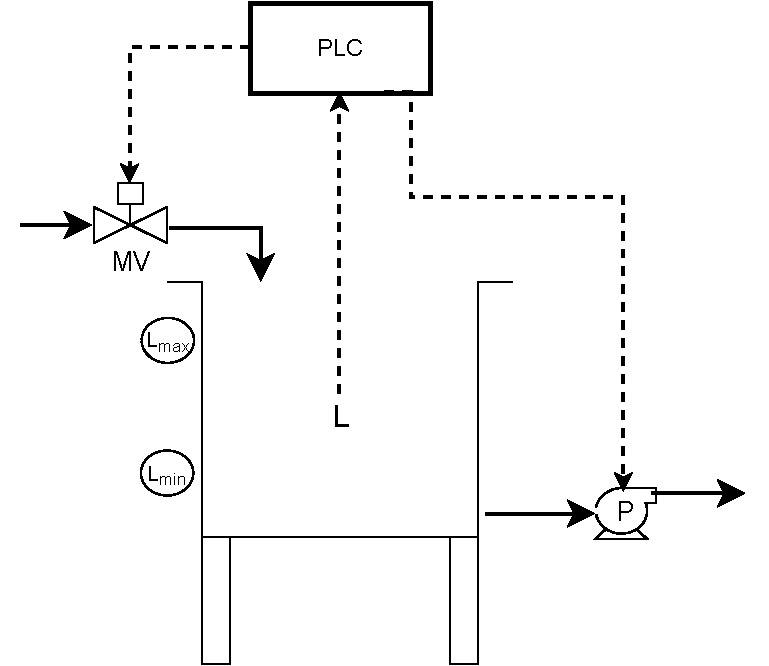
\includegraphics[width=0.50\textwidth]{Figures/FillingTank.pdf}
  \caption{A water tank. The PLC sends control commands to the motor valve (MV) and the pump (P) so that the level of the tank (L) stays within the range $L_{min}$ -- $L_{max}$. }
  \label{fig:CPSRobustness:Motivational}
%\end{wrapfigure}
\end{figure}
%To quantify the robustness of a CPS, we first need to define its model. 
Consider the following model of a CPS containing a water tank with a water level (L), a water pump (P), a motor valve (MV), and a programming logic controller (PLC), as shown in Figure~\ref{fig:CPSRobustness:Motivational}. This system has a physical process state vector $\vec{x}$, a cyber controller state vector $\vec{q}$, a sensor state vector $\vec{y}$, and an actuator state vector $\vec{u}$.

The physical state vector $\vec{x}$ has coordinates $MV$, $L$ and $P$, where $\vec{x}[MV]$ corresponds to the physical state of the motor valve, $\vec{x}[P]$ corresponds to the physical state of the pump, and $\vec{x}[L]$  corresponds to the physical state of the water level of the tank. The variable $\vec{x}[MV]$ can take four values: $\texttt{closed}$, $\texttt{opening}$, $\texttt{open},$ or $\texttt{closing}$. The variable $\vec{x}[P]$ can take two values: $\texttt{on}$ and $\texttt{off}$. Finally, the variable $\vec{x}[L]$ can take any value between $0 ~\mathrm{L}$ and $1200 ~\mathrm{L}$ (the maximum capacity of the tank). %\begin{figure}[t]
%\begin{wrapfigure}[lineheight]{position}{width}
%\end{figure}
Depending on the state of the motor valve $\vec{x}[MV]$, different amounts of water flow into the tank. In turn, the state of the valve $\vec{x}[MV]$ changes when it receives the control input $\vec{u}[MV]$, which can take the values $\texttt{closed}, \texttt{opening},\texttt{open},$ or $\texttt{closing}$.  

The behaviour of the physical process is captured by the following linear time invariant system:
\begin{align}
  \vec{x}[L](k+1)&= \vec{x}[L](k)+Inflow(k)-Outflow(k),\quad \text{where}\\
  Inflow(k)&=\begin{cases}
    0.31,&\quad \text{if $\vec{x}[MV](k)=\texttt{open}$}\\
    0,&\quad \text{if $\vec{x}[MV](k)=\texttt{closed}$}\\
    0.26,&\quad \text{otherwise}\\
  \end{cases}\\
  Outflow(k)&=\begin{cases}
    0.15,&\quad \text{if $\vec{x}[P](k)=\texttt{on}$}\\
    0,&\quad \text{otherwise}\\
  \end{cases}\\
    % \begin{cases}
    %   \vec{x}[L](k)+0.16,&\quad \text{if $(\vec{x}[MV](k),\vec{x}[P](k))=(\texttt{open}$,\texttt{on})}\\
    %   \vec{x}[L](k)-0.15,&\quad \text{if $\vec{x}[MV](k)=\texttt{closed}$,}\\
    %   \vec{x}[L](k)+0.11,&\quad \text{otherwise;}\\
    % \end{cases}\\
  \vec{x}[MV](k+1)&=\vec{u}[MV](k)\\
  \vec{x}[P](k+1)&=\vec{u}[P](k)\\
  \vec{y}[L](k)&=\vec{x}[L](k)
\end{align}
The value of $\vec{y}[L]$ is a measurement of $\vec{x}[L]$, but since it is a cyber component, it can take values above 1200 (although in normal circumstances it remains in the range $[0..1200]$). We leave the initial conditions of the process abstract for now.

The values of the control command for the motor valve $\vec{u}[MV]$ are defined by the controller, which uses $\vec{y}[L]$ to make decisions. The controller itself has a state $\vec{q}$ that has four coordinates: the presumed state the valve $MV$, denoted by $\vec{q}[MV]$, the presumed state of the pump $P$, denoted by $\vec{q}[P]$, the presumed water level of the tank $L$, denoted by $\vec{q}[L]$,  and a timer $\tau$ that the controller uses to approximate the time it takes for the motor valve $MV$ to open or close, denoted $\vec{q}[\tau]$. %These state of the valve, pump and water tank are presumed, because the controller cannot directly observe them

The controller updates its state using $\vec{y}[L]$, and produces the control values $\vec{u}[MV]$ and $\vec{u}[P]$ using $\vec{q}(k)$, with 
\begin{align}
  \label{eq:ControllerStage3}
  \vec{q}[MV](k+1)&=
  \begin{cases}
    \texttt{opening},&\quad \text{if $\vec{q}[MV](k)=\texttt{closed}$ and $\vec{y}[L](k)\leq L_{min}$,}\\
    \texttt{open},&\quad \text{if $\vec{q}[MV](k)=\texttt{opening}$ and $\vec{q}[\tau](k)>T$,}\\
    \texttt{closing},&\quad \text{if $\vec{q}[MV](k)=\texttt{open}$ and $\vec{y}[L](k)\geq L_{max}$,}\\
    \texttt{closed},&\quad \text{if $\vec{q}[MV](k)=\texttt{closing}$ and $\vec{q}[\tau_3](k) >T_3$,}\\
    MV&\quad \text{otherwise;}    
  \end{cases}\\
  \vec{q}[\tau](k+1)&=
\begin{cases}
  1+\vec{q}[\tau](k), &\quad \text{if $\vec{q}[MV](k)=\texttt{opening}$ or $\vec{q}[MV](k)=\texttt{closing}$}\\
  0,&\quad \text{otherwise;}    
\end{cases}\\
\vec{q}[L](k+1)&=\vec{y}[L](k)\\
\vec{q}[P](k+1)&=\texttt{on}\\
\vec{u}[MV](k+1)&=\vec{q}[MV](k+1)\\
\vec{u}[P](k+1)&=\vec{q}[P](k+1)
\end{align}
where $L_{min}=800$, $L_{max}=1000$ and $T=7$. We leave the initial conditions of $\vec{q}$ and $\vec{u}$ abstract for now.

Now that we have a description of the model of the CPS, we define a set of security requirements that determine whether the behaviour of the system is safe or not.

%\subsection{Security Requirements and Additive Attacks}
\subsection*{Security Requirements}
%\begin{wrapfigure}{r}{0.4\textwidth} 
 % \vspace{-1cm}
 \begin{figure}
  \centering
  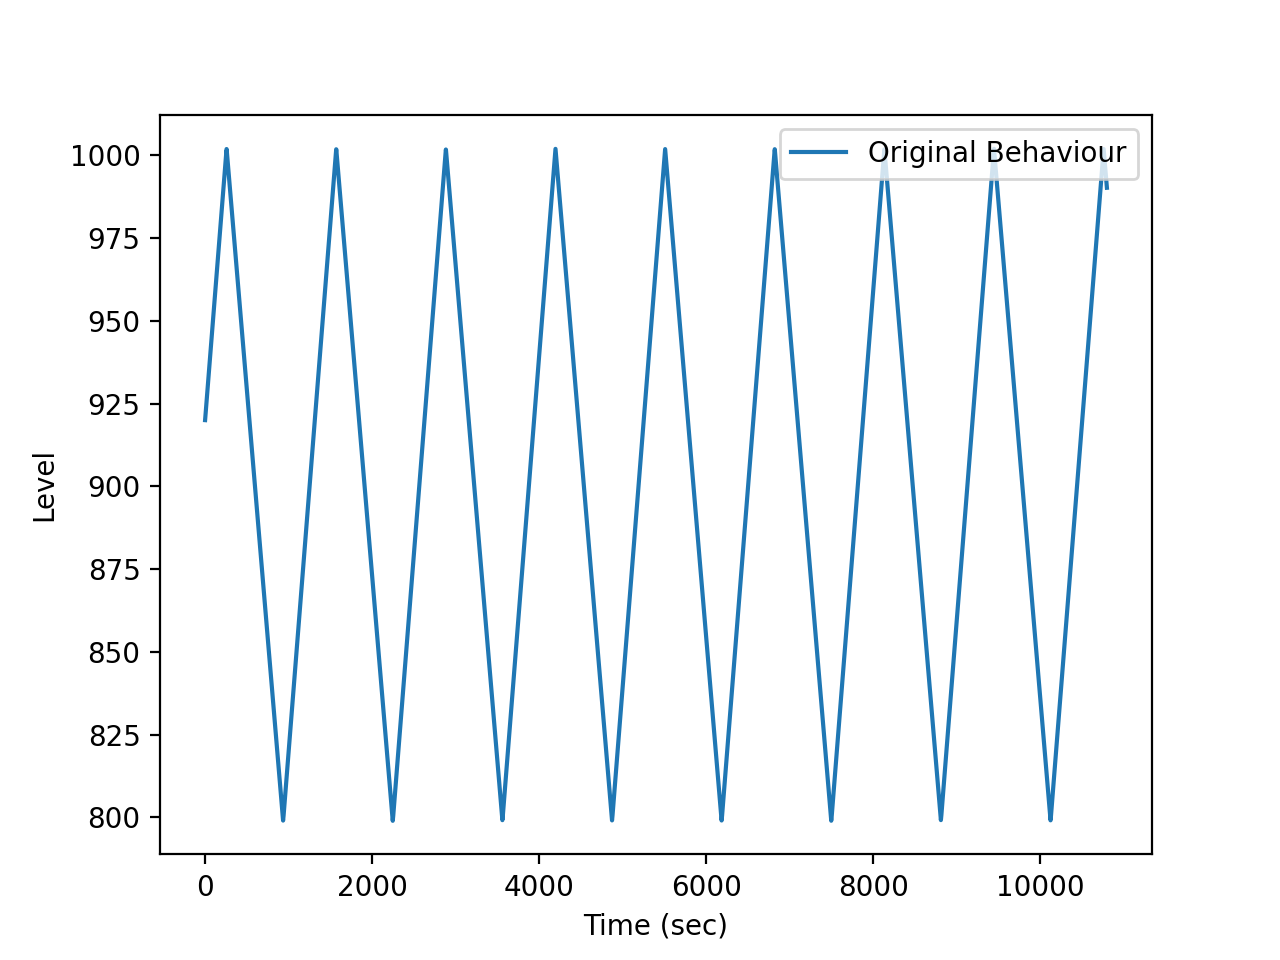
\includegraphics[width=0.5\textwidth]{Figures/Stage3Normal.png}
  %\vspace{-0.25cm}
  \caption{Normal steady state behaviour of the water level of the water tank.}
  \label{fig:CPSRobustness:Stage3Normal}
%   \vspace{-1cm}
% \end{wrapfigure} 
 \end{figure}
We establish two simple security requirements for the water tank: the tank is never empty and the tank never overflows. These requirements protect the integrity of the system: if the tank empties, the pump suffers physical damage due to cavitation, and if the tank overflows, then water spills out, causing a work hazard. Formally, these requirements correspond to the invariants $\Always{\vec{x}[L]< 1200}$ and $\Always{\vec{x}[L]> 0}$, defined by
  \begin{align*}
    \Always{\vec{x}[L]< 1200}&\triangleq \forall k\geq0.\vec{x}[L](k)< 1200,\\
    \Always{\vec{x}[L]> 0}&\triangleq \forall k\geq0.\vec{x}[L](k)> 0.
  \end{align*}
Under normal circumstances, the water level of the tank exhibits the behaviour displayed in Figure~\ref{fig:CPSRobustness:Stage3Normal}. The system in its attack-free state satisfies the security requirements $\Always{\vec{x}[L]< 1200}$ and $\Always{\vec{x}[L]> 0}$.
%\begin{figure}[t]
\subsection*{Testing and Quantifying Robustness}
Now, consider an attacker model where the attacker can replace at any time the value $\vec{y}[L]$ by a value of their choice, or use the real value. This attacker model generates a universe of 64 different \emph{representative classes of attacks}, which define when and what values to use to replace $\vec{y}[L]$. These 64 attacks classes correspond to the paths that the attacker can trigger in the controller by varying the values of $\vec{y}[L]$.  More precisely, the attacker has four options: they can introduce a fake low level value (e.g., 500 L), a fake ok level value (e.g. 800 L), a fake high level value (e.g., 1100 L) or preserve the real water level value. The attacker can choose to use different actions in three main scenarios: when the water level is high, normal, or low. This combination of four ``what" values over three ``when" dimensions defines $4^3=64$ combinations. We explain in detail the generation of attack universes in Section~\ref{sec:CPSRobustness:AttackerCapabilities}. 

We measure the robustness of the system with respect to this attacker model by computing the number of attacks that do not break any of the security requirements. To test an attack in the system, we simulate several operation hours of the system while concurrently simulating the effect of the attack until either the simulation timeouts or the system fails a requirement. After testing, we see that 30 out of 64 attacks break at least one requirement, so the robustness of this system is 34/64 with respect to an attacker that has control of $\vec{y}[L]$. We explain the process of computing robustness in detail in Section~\ref{sec:CPSRobustness:LatentBehaviours}.

\subsection*{Counterattackers}
%So far, we have used a method similar to simulation-based fault-injection to quantify the robustness of the water tank with respect to an attacker that controls the sensor $\vec{y}[L]$; now, 
We now rely on the fundamental observation that an attack $m$ on the original version of the tank reveals a latent system, which we denote $T_m$, and that a transformation $w$ on the latent system $T_m$ reveals another latent system $T^w_m$, which hopefully satisfies all security requirements. In such a case, we say that \emph{$w$ is a counterattack of $m$}. 

A \emph{counterattacker model} is dual to an attacker model. It also requires a ``what" and a ``when" to act. In this scenario, we assume that the counterattacker directly changes the physical state of the pump and the valve, i.e., an operator implements this counterattacker, and they can manually set the coordinate $\vec{x}[P]$ to \texttt{on} or \texttt{off} and the coordinate $\vec{x}[MV]$ to \texttt{open} or \texttt{close}, overriding the commands of the controller. We also assume that the counterattacker can observe the value $\vec{y}[L]$ (which is controlled by the attacker in this scenario). From this counterattacker model, we generate a universe of 729 counterattacks (we explain how we obtain the size of the counterattack universe in Section~\ref{sec:CPSRobustness:CounterAttacks}).  

All 40 successful attacks can be countered, i.e., for each attack $m$ there exists a counterattack $w$ such that the system $T^w_m$ satisfies all the security requirements. Consequently, we say that the system has a \emph{latent robustness} of 64/64; i.e., it is theoretically possible for a counterattacker fitting the counterattacker model to counter every attack of an attacker fitting the attacker model, given that it is possible for the counterattacker to accurately identify that: 1) the system is under attack, and 2) which exact attack is occurring, since apparently similar attacks could have different counterattacks. Assuming the existence of such monitor is impractical; which is why we instead consider a modification of the program of the PLC based on the information that we obtain from the LBA to improve the robustness of the system. In Section ~\ref{sec:CPSRobustness:CaseStudy}, we perform LBA on a system that is more complex than the water tank, and we show how to use the relations between attacks and counterattacks obtained via LBA to propose repairs that improve the robustness of the model.  

\section{Cyber-Physical Systems, Physical Requirements and \\Attacker Models}
% Our main objective is to define a flexible testing method to determine how well the integrity of the process of a CPS is preserved in the presence of attackers. For this purpose, we now define formal notions of \emph{CPS state}, \emph{single-cycle semantics}, and \emph{physical integrity requirements}.
%\todo[inline]{Small intro that explains what this section is}
%Traditional IT security mechanisms such as authentication and message integrity are insufficient for CPS security. %However, as stated in \cite{CPSAttacksAgainstPCS}, 
The major difference between CPSs and IT systems is the interaction with the physical world. We share the view of Gollmann \emph{et al.} \cite{CPSSecVinyl}, who state that CPSs security is {specifically} concerned with attacks that cause some physical impact; i.e., attack that affect the integrity of the physical process beyond repair. The robustness of a system is a measure of tolerability to those attacks that target integrity. 
%Traditional IT security mechanisms (e.g., firewalls, encryption, signatures, etc.) normally do not account for physical parts of the system, making them ineffective when faced against attacks that either target or interact with the physical components of CPSs. In this section, we present an Information Flow (IF) inspired integrity analysis for CPSs which accounts for the physical process.

In this section, we present a framework to quantify the robustness of CPSs. This framework consists of several parts:
\begin{enumerate}
  \item a discrete model for CPSs and their semantics; 
  \item a description of physical security requirements;
  \item a formalisation of attacker models and attacks for our CPS models;
  \item a formulation of counterattacker models and counterattacks, dual to those of attackers and attacks;
  \item a quantitative notion of robustness and latent robustness based on physical security requirements, attacker models and counterattacker models.
\end{enumerate}

\subsection{A Discrete Model for CPSs}
Figure \ref{fig:CPSRobustness:IFCPS} presents an extended version of the \emph{supervisor model} \cite{doi:10.1137/0325013}, which serves as the starting point for our modelling framework. 
\begin{figure}
\centering
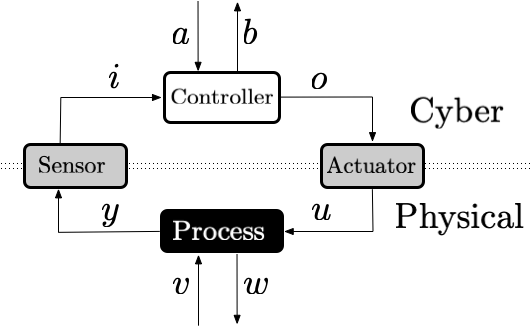
\includegraphics[width=0.45\textwidth]{Figures/IFCPS}
\caption{Extended supervisor model accounting for external inputs and outputs in both cyber and physical components.}
\label{fig:CPSRobustness:IFCPS}
\end{figure}
Our CPS model consists of four subsystems: the \emph{controller}, an open, discrete cyber system; the \emph{process}, a linear-time invariant physical system; and two sets of cyber-and-physical interface systems: the \emph{sensors} and the \emph{actuators}. The vector $\vec{q}$ models the current state of the controller, and $\vec{x}$ models the current state of the process. The vector $\vec{i}$ models cyber input measurements and the vector $\vec{o}$ models cyber control outputs; they respectively model the internal communication channels between controller and sensors, and between controller and actuators. Similarly, the vector $\vec{u}$ models the physical control inputs and the vector $\vec{y}$ models physical measurements; these vectors respectively model the internal communication channels between the process and actuators, and between the process and sensors. 

The cyber network input $\vec{a}$ and the cyber network output $\vec{b}$ enable communication between controllers, and enable CPS composition on the cyber side. Similarly, the physical network input $\vec{v}$, and the physical network output $\vec{w}$ model physical channels that connect modules of a larger physical system, enabling the composition of CPS on the physical side. For example, when two water tanks $T_1$ and $T_2$ are connected by a pipe, the outgoing flow from $T_1$ to $T_2$ (a component of $\vec{w}$ for $T_1$) should translate into the incoming flow from $T_1$ to $T_2$ (a component of $\vec{v}$ for $T_2$). 

\begin{definition}[States of a CPS]
\label{def:CPSRobustness:States}
A \emph{state of a CPS} $\pi$ is the coupling of the components of such CPS; formally, 
\begin{align}
\pi=(\vec{a},\vec{b},\vec{i},\vec{o},\vec{u},\vec{y},\vec{v},\vec{w},\vec{q},\vec{x}).
\end{align}
%$(\vec{a},\vec{b})$ is the state of the network, $(\vec{i},\vec{o},\vec{u},\vec{y})$ is the state of the channels, $(q,x)$ is the \emph{hidden} state of the controller and the process. 
%\todo[inline]{@All: for this paper this notation is fine because we do not write things like $\pi[\vec{x}[smt[smt2[smt3]]]]$ or $\pi[\vec{x}][smt][smt2]...$ which is horrible, we write $\pi[\vec{x}[L]]$,though.}
Let $\vec{A}$ be the \emph{range} of $\vec{a}$; i.e., the set of values that $\vec{a}$ can take. Similarly, we define $\vec{B}$, $\vec{I}$, $\vec{O}$, $\vec{U}$, $\vec{Y}$,  $\vec{V}$, $\vec{W}$ $\vec{Q}$, and $\vec{X}$ as the ranges of $\vec{b}$, $\vec{i}$, $\vec{o}$, $\vec{u}$, $\vec{y}$, $\vec{v}$, $\vec{w}$, and $\vec{q}$, respectively. We defined the set $\Pi$ of the CPS states by 
\begin{align}
  \Pi\triangleq \vec{A}\times\vec{B}\times\vec{I}\times\vec{O}\times\vec{U}\times\vec{Y}\times\vec{V}\times\vec{W}\times\vec{Q}\times\vec{X}.  
\end{align}
Finally, we informally define the set of \emph{coordinates} $\mathbb{C}$ to be the set of elements in the CPS model that have no subcomponents. For example, the vector $\vec{u}$ from Section~\ref{sec:CPSRobustness:example} has two subcomponents, $\vec{u}[MV]$ and $\vec{u}[P]$, so $\vec{u}$ is not a coordinate, but both $\vec{u}[MV]$ and $\vec{u}[P]$ individually are. We refer to the elements of $\mathbb{C}$ as the \emph{coordinates} of the CPS.
\end{definition}

% \begin{minted}{haskell}
% data P1 =
%   P1 {
%     a1::Maybe Bool, -- P2 asking to start/stop inflow of water
%     b1::Maybe Bool, -- P1 informing P2 about the state of p1
%     y1::Float, -- water level in ml
%     ov1::Maybe Bool, -- control signal to v1
%     op1::Maybe Bool, -- control signal to p1
%     p1::Bool, -- physical state of p1
%     v1::Bool, -- physical state of v1
%     t1::Int -- time step
%     } 
% \end{minted}

Informally, the semantics of a CPS is the following: the process, whose state is $\vec{x}$, is observed by the sensor, yielding the physical observation $\vec{y}$; the sensor transforms $\vec{y}$ into the cyber input observation $\vec{i}$. The controller, whose state is $\vec{q}$, receives $\vec{i}$ and a cyber network input $\vec{a}$, and produces a cyber network output $\vec{b}$ and a cyber control command $\vec{o}$. The cyber command $\vec{o}$ is then transformed into a physical control command $\vec{u}$ by the actuator. The process, whose state is $\vec{x}$, reacts to $\vec{u}$ and to some physical network input $\vec{v}$, returning a physical network output $\vec{w}$ while updating its state. The cycle repeats by having the sensor observe the physical state $\vec{x}$ to produce $\vec{y}$ once more. We now formally define how a state of the CPS evolves over time. 
{
\begin{definition}[Single-Cycle Semantics]
\label{def:CPSRobustness:SingleCycleSemantics}
Let $\Pi\triangleq \vec{A}\times\vec{B}\times\vec{I}\times\vec{O}\times\vec{U}\times\vec{Y}\times\vec{V}\times\vec{W}\times\vec{Q}\times\vec{X}$ be the set of states of the CPS; we assume the existence of the following functions,
\begin{itemize}
\item $\delta_{\vec{Q}}\colon \vec{Q}\times \vec{A}\times \vec{I} \rightarrow \vec{Q}$, the transition function of the controller,
%\item $\beta_{\vec{Q}}\colon \vec{Q}\times \vec{A}\times \vec{I} \rightarrow \vec{B}$, the network output function of the controller,
%\item $\theta_{\vec{Q}}\colon \vec{Q}\times \vec{A}\times \vec{I} \rightarrow \vec{O}$, the digital control output function of the controller,
\item $\beta_{\vec{Q}}\colon \vec{Q}\rightarrow \vec{B}$, the network output function of the controller,
\item $\theta_{\vec{Q}}\colon \vec{Q}\rightarrow \vec{O}$, the cyber control output function of the controller,
\item $\theta_{\vec{Y}}\colon \vec{Y} \rightarrow \vec{I}$, the translation function of the sensor,
\item $\theta_{\vec{O}}\colon \vec{O} \rightarrow \vec{U}$, the translation function of the actuator,
\item $\delta_{\vec{X}}\colon \vec{X} \times \vec{U}\times \vec{V} \rightarrow \vec{X}$, the transition function of the process,
% \item $\beta_{\vec{X}}\colon \vec{X} \times \vec{U}\times \vec{V} \rightarrow \vec{W}$, the physical effect function of the physical component.
%\item $\theta_{\vec{X}}\colon \vec{X}\times \vec{U}\times \vec{V} \rightarrow \vec{Y}$, the physical output function of the process.
\item $\beta_{\vec{X}}\colon \vec{X}\rightarrow \vec{W}$, the physical effect function of the process,
\item $\theta_{\vec{X}}\colon \vec{X}\rightarrow \vec{Y}$, the physical output function of the process.
\end{itemize} 
% These functions help us control the flow of information; e.g., values of physical variables must go through some sensor to be received by a controller, so a flow from $\vec{x}$ to $\vec{q}$ cannot occur directly. 

We define the single-cycle semantics function $\TheSystem\colon \Pi \rightarrow \Pi$ that describes the evolution of the state $\pi=(\vec{a},\vec{b},\vec{i},\vec{o},\vec{u},\vec{y},\vec{v},\vec{w},\vec{q},\vec{x})$ of the CPS by
\begin{align}
\TheBehaviourOf{\pi}&\triangleq\left((\vec{a'},\vec{b'},\vec{i'},\vec{o'},\vec{u'},\vec{y'},\vec{v'},\vec{w'},\vec{q'},\vec{x'})\right), 
\end{align}
where $\vec{a'}$ and $\vec{v'}$ are external inputs, and 
\begin{gather*}
%\vec{o'}=\theta_{\vec{Q}}(\vec{q},\vec{a},\vec{i}),\quad 
\vec{o'}=\theta_{\vec{Q}}(\vec{q}),\quad 
\vec{q'}=\delta_{\vec{Q}}(\vec{q},\vec{a},\vec{i}),\quad 
%\vec{b'}=\beta_{\vec{Q}}(\vec{q},\vec{a},\vec{i}),\\
\vec{b'}=\beta_{\vec{Q}}(\vec{q}),\\
\vec{x'}=\delta_{\vec{X}}(\vec{x},\vec{u},\vec{v}),\quad
%\vec{y'}=\theta_{\vec{X}}(\vec{x},\vec{u},\vec{v}),\quad \vec{w'}
\vec{y'}=\theta_{\vec{X}}(\vec{x}),\quad 
%\vec{w'}=\beta_{\vec{X}}(\vec{x},\vec{u},\vec{v}),\\
\vec{w'}=\beta_{\vec{X}}(\vec{x}),\\
\vec{u'}= \theta_{\vec{O}}(o),\quad\vec{i'}=\theta_{\vec{Y}}(\vec{y}).
\end{gather*}
%i.e. for all $k$, $\vec{i}(k)=\vec{y}(k)$ and $\vec{u}(k)=\vec{o}(k)$. 
The evolution over $k+1$ cycles is defined by the iteration of $\TheSystem$, {i.e.}, 
%\begin{align}\label{eq:kCycles}
$\TheSystem_{k+1}= \TheSystem \circ \TheSystem_{k}.$
%\end{align}
Finally, we define $\TheBehaviourOf{\pi}_{0}=\pi$ for all states $\pi \in \Pi$. Under this definition, the \emph{normal behaviour} of the CPS is characterised by the infinite sequences $(\pi_0, \pi_1, \ldots)$ where $\pi_{k+1}\triangleq\TheBehaviourOf{\pi_k}$ and $\pi_0$ is an initial state.%; equivalently $\pi_{k}\triangleq \TheBehaviourOf{\pi_0}_k$.
\end{definition}
}
Because a CPS itself does not create values for $\vec{a}$ and $\vec{v}$, we need a stream of network inputs $(\vec{a_0}, \vec{a_1}, \ldots)$ and a stream of physical effects $(\vec{v_0}, \vec{v_1}, \ldots)$ to advance the system. Usually, $\vec{a}$ is the translation of a network output $\vec{b}$ given by another CPS; similarly, $\vec{v}$ is the translation of a physical output $\vec{w}$ from another system. If the functions $\delta_{\vec{Q}}$ and $\delta{\vec{X}}$ respectively ignore $\vec{a}$ and $\vec{v}$ for their computation, then we say that the CPS is \emph{closed}.
Henceforth, we assume that the CPS (or composition of CPSs) we are working with is closed. We study a closed CPSs composition in Section~\ref{sec:CPSRobustness:CaseStudy}.

{\color{red} From the perspective of coalgebras, this definition of latent behaviour implies that the whole state is observable from the modelling perspective. Implicitly, we are working with a functor $F(X)=\Pi\times X$, modelling the CPS using the $F$-coalgebra $(\Pi,(\id,\TheSystem))$. 
%The final $F$-coalgebra is $(\sigma F, 1_F)$ with $\sigma F=\Pi^\infty$, i.e., the set of infinite sequences of elements of $\Pi$ and $1_F=(\head,\tail)$. 
% We adjust the visibility by adjusting the functor: a functor $G(X)=\vec{Y}\times X$ restricts the visibility to the values read by sensors by $(\Pi,(\vec{y},\TheSystem))$
}

In the following, we define a notion of integrity based on security requirements over physical components. We also discuss the attacker models we consider in this work, and a method to systematically generate attacks.

\subsection{Physical Integrity Requirements}{
  % Before we formally define attackers and their attacks, we introduce the notion of \emph{physical integrity requirement}. 
We use \emph{physical integrity requirements} to determine when the behaviour of the process $\vec{x}$ has deviated critically, and becomes unsafe, independently of whether the system is under attack or not. Formally, physical integrity requirements model \emph{safety properties} over the physical state of the CPS.
\begin{definition}[Physical Integrity Requirement]
  \label{def:CPSRobustness:IntegrityRequirement}
  Let $\Pi$ be the set of states of the CPS. A \emph{physical integrity requirement} is a finite state automaton $\TheRequirement=(S,\delta,F,s_0)$, where $S$ is a set, $\delta\colon S\times \vec{X}\rightarrow S$ is the transition function, $F\subseteq S$ marks critical states, and $s_0\in S$ is the initial state. Given a possibly infinite sequence of states of the CPS $\omega=(\pi_0,\pi_1 \ldots)$, we say that \emph{$\omega$ fails the physical integrity requirement $\TheRequirement$} if and only if there exists a finite prefix of $\omega$, say $(\pi_0,\ldots\pi_n)$, such that the sequence $(\pi_0[\vec{x}],\ldots, \pi_n[\vec{x}])$ is rejected by $\TheRequirement$. Henceforth, we refer to physical integrity requirements simply as \emph{physical requirements}. 
  
The \emph{behaviours of the CPS} are the infinite sequences $(\pi_0, \pi_1, \ldots)$ where $\pi_{k+1}=\TheBehaviourOf{\pi_k}$ and $\pi_0$ is an initial state. The CPS \emph{satisfies  $\TheRequirement$} iff all its behaviours satisfy $\TheRequirement$. We expect the attack-free CPS to satisfy all physical requirements.
  %Under this definition, physical requirements correspond to safety properties.
\end{definition}
  %\todo[inline]{Awesome! now we can model a requirement that states that the water level of the tank must not remain low for large periods of time, or the pump would burn.}]
   

% \color{blue}
% \todo[inline]{@All: this section in blue remains from the workshop version. We could keep it, unless you feel it does not fit the tone of the paper.}
\subsection{Attacker Models} 
Clarkson and Schneider state in \cite{QuantitativeIntegrity} that they know of no widely accepted definition of integrity, but they remark that an ``informal definition seems to be the `prevention unauthorized modification of information'." Clarkson and Schneider use two formal notions to characterise and quantify \emph{corruption}, i.e., the damage to integrity. One notion is \emph{contamination}, a generalisation of taint analysis that tracks information flows from untrusted inputs to outputs that are supposed to be trusted. The other notion is \emph{suppression}, which occurs when implementation outputs omit information about correct outputs with respect to the specification. Contamination is dual to information leakage under the Biba duality; however, there is no apparent Biba dual to suppression \cite{BibaIntegrity}. 
%Both contamination and suppression are present in CPSs. For example physical attackers can contaminate the state of physical components by directly interacting with them (e.g. an attacker jamming a pump), and cyber attackers can suppress the communication between controllers (e.g. by launching a mitm attack).
In this work, we want to test whether any corruption generated by contamination of information affects the integrity of the behaviour of the system. To that end, we %want to minimise the restrictions we impose over attackers; more precisely, we believe 
give attackers the ability to either: 1) alter the value of the coordinates they control by means of arbitrary substitution, or 2) leave the current value be. We only impose a minimal type-checking restriction: the input provided by the attacker must be in the range of the corrupted coordinate, or the behaviour of the system becomes ill-defined. We allow attackers to have some view over the current state of the system, so they can decide when and to corrupt the components they control. Attackers that contaminate information using other methods besides arbitrary substitutions are beyond the scope of this work, e.g., attackers that contaminate data by adding noise (although they are compatible with LBA, since these attacks can be described as spatial transformations).  

%\todo[inline]{Ultimately, it does not matter whether the attacker wants to reuse the current value in some way(contaminate), or set a fixed value (suppress), because only some values matter, and they only matter under certain conditions.}
%\todo[inline]{This discussion on information flow should be very vague, considering that we do not really use entropy or anything else related to information flow. It makes for an interesting introduction though; we should just be careful that the readers don't get the wrong idea.} 


% In Section~\ref{sec:CPSRobustness:example} we hinted the possibility of describing attacks as vectors. In this section, we discuss in more detail the meaning of the bases and the coefficients of attacks.
Following the methodology of LBA, we aim to compose the single cycle semantics function $\TheSystem\colon\Pi\rightarrow\Pi$ from Definition~\ref{def:CPSRobustness:SingleCycleSemantics} with a spatial transformation $m\colon \Pi\rightarrow\Pi$ (which models some attack) to reveal the transition function $\TheSystem\circ m\colon\Pi\rightarrow\Pi$ of a latent system which models the CPS under the attack $m$. In the following, we show how to describe attacks as both vectors and spatial transformations, and we show how to systematically generate them from an attacker model.

\subsubsection{Attacker Models}
We now show how an attacker model --which describes how an attacker may interact with the system and when-- generates a set of attacks. Each attacker model is composed by a \emph{basis} and a set of \emph{coefficients}. The \emph{basis} reflects the visibility of the attacker over the current state of the system, helping them decide ``when'' to attack. The \emph{coefficients} determine the actions that the attacker uses when interacting with the system, and they define the ``how'' an attacker attacks.

\begin{definition}[Attack Basis]
  \label{def:CPSRobustness:AttackBasis}
Let $\Pi$ be the set of states of the CPS. An \emph{attack basis} is a \emph{finite} partition $\sum_{i=1}^n \Pi_i$ of $\Pi$; i.e., for $1\leq i,j \leq n$, $\Pi_i$ is non-empty, $\Pi_i$ and $\Pi_j$ are pairwise disjoint, and the union of all $\Pi_i$ is $\Pi$. We often refer to an element of the partition $\Pi_i$ by its characteristic predicate; i.e., we write $\Pi_i(\pi)$ instead of $\pi\in \Pi_i$.

The most granular base is given by the individual elements of $\Pi$, and it models an attacker with absolute visibility: this attacker always knows the value of every component of the current state, and can act differently at every state if they so wish. The least granular base is given by $\Pi$ itself, and it models an attacker with no visibility over the current state; this attacker repeats the same action over and over, independently of the current state.
\end{definition}
\begin{example}
  \label{ex:CPSRobustness:AttackBasis}
  For the water tank from Section~\ref{sec:CPSRobustness:example}, we define the base $[LL, OK, HH]^T$, where 
  \begin{align*}
    {LL}&\triangleq\set{\pi| \pi[\vec{x}[L]]<L_{min}},\\
    {HH}&\triangleq\set{\pi| \pi[\vec{x}[L]]>L_{max}}, and\\
    {OK}&\triangleq\set{\pi|L_{min} \leq \pi[\vec{x}[L]]\leq L_{max}}. 
  \end{align*} 
  The base $[LL, OK, HH]^T$ models the visibility of an attacker that can always determine whether the current state of the system satisfies $LL$, in $OK$ or in $HH$. These bases can bypass normal observation assumptions: in this example, the attacker does not observe the value measured by the sensor $\pi[\vec{y}[L]]$; instead, we assume that they observe the real level of the water tank $\pi[\vec{x}[L]]$ by some alternative means. %We refer to $\set{\pi\in \Pi| \pi[\vec{x}[L]]>L_{max}}$ by $(\vec{x}[L]>L_{max})$ and we refer to $\Pi$ by $\True$.
\end{example}

Informally, the coefficients provided by an attacker model are actions that may affect multiple coordinates simultaneously, and they define how the attacker interacts with the system. We want attackers to be capable of setting any values on the components they control. Unfortunately, we face a typical coverage problem of system testing: many different values exercise the same execution paths, and some paths may be exercised only by very specific inputs. For our examples, we manually choose these representative values to maximise the coverage of testing, but a selection process for the values that maximise coverage is beyond the scope of this work.

Before we formally define attack coefficients, we introduce a two auxiliary concepts: {constant transformations of coordinates} and the {idempotent monoid generated by combining those constant transformations.
\begin{definition}[Constant Transformations of a Coordinate]
  Let $c\in \mathbb{C}$ be a coordinate of the CPS whose range is $C$ and let $v$ be a representative value in $C$; we define the \emph{constant transformation of $c$ to $v$}, denoted $\const^{c}_{v}\colon \Pi\rightarrow \Pi$, for all $\pi \in \Pi$ and $c'\in \mathbb{C}$ by
  \begin{align}
    \const^{c}_{v}(\pi)[c']& \triangleq 
    \begin{cases}
     v, &\quad \text{if $c'=c$,}\\
     \pi[c']&\quad \text{otherwise.}
    \end{cases} 
  \end{align} 
\end{definition}
% The natural choice for this set of coefficients is the monoid $(\Pi\rightarrow \Pi, \circ, \id)$, because it enables attack composition. However, 
% An attacker model contains a finite set of \emph{representative values}
% By combining a finite set of coefficients and a finite basis given by an attacker model, we generate a finite number of attacks. Formally, we generate an {idempotent monoid} using constant transformations of coordinates.%, henceforth named $\IMCT$.

% \begin{definition}[\textbf{I}dempotent \textbf{M}onoid Generated by \textbf{C}onstant \textbf{T}ransformations in one coordinate (\textbf{$\IMCT$})]
\begin{definition}[Idempotent Monoid Generated by Constant Transformations of Coordinates {$\IM{\Gamma_{\mathcal{K}}}$}]
  \label{def:CPSRobustness:IdempotentMonoid}
% generated from a finite set of \emph{representative values}. More precisely, let $\vec{C}$ be the range of $c$; given some representative value $v\in \vec{C}$, there exists a transformation $\const^{c}_{v}\in \Gamma_c$.

% Now, each coordinate $c$ defines a set of generators $\const(\Gamma_c)$, formally defined by
% \begin{align}
%   \const(\Gamma_c)\triangleq \set{\const^{c}_{v} | v\in\Gamma_c}.
% \end{align}
Let $\mathcal{K}\subseteq\mathbb{C}$ be a set of coordinates, and let $\Gamma_\mathcal{K}$ be a \emph{finite} set of constant transformations of the coordinates in $\mathcal{K}$. We generate the monoid $(\IM{\Gamma_{\mathcal{K}}},\circ,\id)$ %by choosing $\mathcal{K}=\mathbb{C}$, and 
by closing %the union of all $\Gamma_c$ in the family $\Gamma_{\mathbb{C}}$ 
$\Gamma_{\mathcal{K}}$ under function composition; the unit of the monoid is the identity function $\id$, and the operation is function composition $\circ$. The elements of this monoid are our \emph{attack coefficients}, and they describe the actions that the attacker can perform.

%$\AsSequence{\ucup_{c\in \mathbb{C}}\const(\Gamma_c)}$
% \begin{definition}[Single Component Transformations]
% Let $c\colon \Pi\rightarrow \Pi$. We say that $c$ is a \emph{single-component transformation (on $\sigma$)} of the elements of $\Pi$ if and only if $c=\id$, or there exists one and only one component $\sigma$ such that c
% \begin{align}
%   c(\pi)[\sigma]=\pi[\sigma],
% \end{align} 
% and $\sigma$ has no subcomponents. 
%Due to properties of the monoid and because 
Each transformation $t\in \IMCT$ is finitely generated and unambiguously pairs each coordinate $c\in \mathbb{C}$ with either $\id$ or with some constant transformation $\const^{c}_{v}$ in $\Gamma_{\mathcal{K}}$.  We denote this association by $t[c]$. If $t[c]=\id$, then $t$ does not act on the coordinate $c$, and if $t[c]=\const^{c}_{v}$, then $t(\pi)[c]=v$ for all $\pi \in \Pi$.
\end{definition}
An attacker model is a pair of a set of constant transformations of coordinates and a basis.
\begin{definition}[Attacker Model]
  Let $\Gamma_\mathcal{K}$ be a set of constant transformations of coordinates for some set of coordinates $\mathcal{K}$, and let $\sum_{i=1}^n\Pi_i$ be a basis; the pair $\mathcal{A}=(\Gamma_{\mathcal{K}}, \sum_{i=1}^n\Pi_i)$ defines the \emph{attacker model} for attackers that have visibility $\sum_{i=1}^n\Pi_i$ over the CPS and that are capable of applying the transformations in $\IM{\Gamma_\mathcal{K}}$ %\subseteq \IM{\Gamma_\mathbb{C}}$ 
   to the states of the CPS, \emph{but only those transformations}. %Any transformations that are not in the submonoid $\IM{\Gamma_\mathcal{K}}$ are beyond the capabilities of attacker that fit this model.%, \emph{but only those}.
   
   The attacks generated by the attacker model $(\Gamma_{\mathcal{K}}, \sum_{i=1}^n\Pi_i)$ are the vectors whose coefficients are elements of $\IM{\Gamma_\mathcal{K}}$ and whose basis is $\sum_{i=1}^n\Pi_i$. 
   % The attacks associated to the attacker model  be the idempotent submonoid of constant transformations on coordinates constructed following Definition~\ref{def:CPSRobustness:IMCT} using $\mathcal{C}$ and $\Gamma_{C}$,is generated using the components defines an \emph{attacker model} . 
 \end{definition}
 %\todo[inline]{@Eric: maybe parametrise the $\IMCT$ in its definition??}
 
% We finally define attacks by combining attack coefficients in $\IMCT$ and the predicates in the basis $\sum\Pi$.
\begin{definition}[Attack]
  \label{def:CPSRobustness:Attack}
Given an attacker model $\mathcal{A}=(\Gamma_{\mathcal{K}}, \sum_{i=1}^n\Pi_i)$,
 %generated by the representative values $\Gamma_c$ for each $c\in \mathbb{C}$, 
 an \emph{attack} $\vec{m}\colon \Pi\rightarrow \Pi$ \emph{generated by $\mathcal{A}$} is a linear combination
\begin{align}
  \vec{m}=t_1\Pi_1 + t_2\Pi_2 + \ldots + t_n\Pi_n,
\end{align} 
where $t_1, \ldots, t_n\in\IMCT$ is a choice of $n$ coefficients. The attack $\vec{m}$ implements a function defined for $\pi\in \Pi$ by
\begin{align}
  \label{eq:AttackVector}
  \vec{m}(\pi)=
    \begin{cases}
      t_1(\pi), &\quad\text{if $\pi\in \Pi_1$;}\\
      \ldots&\quad\ldots\\
      t_n(\pi), &\quad\text{if $\pi\in \Pi_n$.}
    \end{cases}
\end{align}
For convenience, we write $\vec{m}$ using vectors as follows: 
\begin{align}
  \vec{m}(\pi)=
  %[t_1,\ldots,t_n]
  \begin{bmatrix}
    t_{1} \\
    \vdots \\
    t_{n}
  \end{bmatrix}
  \cdot
  \begin{bmatrix}
    \Pi_{1} \\
    \vdots \\
    \Pi_{n}
  \end{bmatrix}.
\end{align} 
We can scale an attack $\vec{m}\colon \Pi\rightarrow \Pi$ by $t\in \IMCT$ to obtain the attack $t\vec{m}\colon \Pi\rightarrow \Pi$, defined for $\pi\in \Pi$ by
\begin{align}
  t\vec{m}(\pi)\triangleq
  %[t_1,\ldots,t_n]
  \begin{bmatrix}
    t\circ t_{1} \\
    \vdots \\
    t\circ t_{n}
  \end{bmatrix}
  \cdot
  \begin{bmatrix}
    \Pi_{1} \\
    \vdots \\
    \Pi_{n}
  \end{bmatrix}.
\end{align} 
The set of all attacks generated by the attacker model $\mathcal{A}$ is $\AsSequence{\mathcal{A}}$.

We can also combine attacks --i.e., attack addition-- using function composition, which is \emph{not commutative}. The sum of attacks using the same basis corresponds to the composition of their coefficients. However, the sum of attacks with different bases requires a common basis: given attacks $\vec{m}_1$ and $\vec{m}_2$ whose respective bases are $\sum_{i=1}^n\Pi_i$ and $\sum_{i=1}^m\Pi'_i$, 
we define the common basis $(\sum_{i=1}^n\Pi_i)(\sum_{i=1}^m\Pi'_i)$ by 
\begin{align}
  \left(\sum_{i=1}^m\Pi'_i\right)\left(\sum_{i=1}^n\Pi_i\right)\triangleq \sum_{j=1}^m\sum_{i=1}^n(\Pi'_j\cap\Pi_i);
\end{align}
% To compose $\vec{m}_1$ and $\vec{m}_2$ it is convenient to express them as linear combinations as follows

% \begin{align*}
%   \vec{m}_2\circ \vec{m}_1&=(t'_1\Pi'_1 + \ldots + t'_m\Pi'_m)(t_1\Pi_1 + \ldots + t_n\Pi_n)\\
%   &=t'_1\Pi'_1(t_1\Pi_1 + \ldots + t_n\Pi_n)+ \ldots t'_m\Pi'_m(t_1\Pi_1 + \ldots + t_n\Pi_n)\\
%   &=(t'_1\circ t_1)(\Pi'_1\cap\Pi_1) + \ldots (t'_1\circ t_n)(\Pi'_1\cap\Pi_n)+ \ldots \\
%   &+(t'_m\circ t_1)(\Pi'_m\cap\Pi_1) + \ldots + (t'_m\circ t_n)(\Pi'_m\cap\Pi_n).
% \end{align*} 
%in its vectorial form it corresponds to
so the sum of $\vec{m}_2$ and $\vec{m}_1$ is defined by
\begin{align}
  (\vec{m}_2+\vec{m}_1)(\pi)\triangleq(\vec{m}_2\circ\vec{m}_1)(\pi)\triangleq
  %[t_1,\ldots,t_n]
  \begin{bmatrix}
    t'_{1}\circ t_1 \\
    \vdots \\
    t'_{1}\circ t_n\\
    \vdots \\
    t'_{m}\circ t_1 \\
    \vdots \\
    t'_{m}\circ t_n
  \end{bmatrix}
  \cdot
  \begin{bmatrix}
    \Pi'_{1}\cap\Pi_{1} \\
    \vdots \\
    \Pi'_{1}\cap\Pi_{n}\\
    \vdots \\
    \Pi'_{m}\cap\Pi_{1} \\
    \vdots \\
    \Pi'_{m}\cap\Pi_{n}\\
  \end{bmatrix}.
\end{align} 
Finally, if the states of the CPS must satisfy a physical invariant $\mathcal{I}\colon \vec{x}\rightarrow\bool$, then we say that an attack $m$ is \emph{physically impossible} if there exists some state $\pi\in \Pi$ such that $\pi[\vec{x}]$ satisfies $\mathcal{I}$, but $\vec{m}(\pi)[\vec{x}]$ does not. If we do not impose this restriction, then attackers that act on physical components would be able to break the laws of physics. This restriction does not apply for cyber components, but it illustrates that we sometimes need to filter out attacks generated from a model. % with arbitrary criteria. 
Since we focus on cyber attackers, we do not exclude any attacks generated by our attacker models. %The definition of these filtering criteria  are beyond the scope of this work. 
% \todo[inline]{Physical invariants may go beyond $\vec{x}$, but I'll just keep them restricted to $\vec{x}$ for now.}
\end{definition}
\begin{example}
  \label{ex:CPSRobustness:attack}
  In general, the pair $(\Gamma_{\emptyset}, \Pi)$ models a passive attacker, since the only attack of this model is $\vec{id}=[\id]\cdot[\True]$; i.e. an attack that does not change the state. %, since $\id$ is the only element of the monoid $\IM{\Gamma_{\emptyset}}$. 

  Now, consider the attacker model $(\Gamma_{\vec{y}[L]},\set{LL,OK,HH})$ in the context of the water tank of Section~\ref{sec:CPSRobustness:example}, where
  \begin{align}
    \Gamma_{\vec{y}[L]}=\set{\const^{\vec{y}[L]}_{500}, \const^{\vec{y}[L]}_{800},  \const^{\vec{y}[L]}_{1100}}.
  \end{align}
  We give the attacker model the {representative values} $500~\mathrm{L}$, $800~\mathrm{L}$ and $1100~\mathrm{L}$ for $\bar{y}[L]$ because each of these values triggers different paths in the controller: $500~\mathrm{L}$ activates the paths where the water level is low, $800~\mathrm{L}$ activates those paths where the water level is normal, and finally the value $1100~\mathrm{L}$ covers the paths where the water level is high.

  This attacker model generates attacks that affect $\vec{y}[L]$  depending on whether the state satisfies $LL$, $OK$ or $HH$; 
  however, their effects over $\vec{y}[L]$ are limited to $\IM{\Gamma_{\vec{y}[L]}}=\left\{\id, \const^{\vec{y}[L]}_{500}, \const^{\vec{y}[L]}_{800}, \const^{\vec{y}[L]}_{1100}\right\}$. Each attack is a combination of the basis $[LL, OK, HH]^T$ and the coefficients in $\IM{\Gamma_{\vec{y}[L]}}$, so this attacker model generates 64 attacks, given by the combination ${\left|\IM{\Gamma_{\vec{y}[L]}}\right|}^{\left|\set{LL,OK,HH}\right|}=4^3$. For example, we define $\vec{m}$ by
\begin{align}
  \vec{m}=
  \begin{bmatrix}
    \id \\
    \const_{500} \\
    \const_{500}
  \end{bmatrix}
  % [\id,\const_{500},\const_{500}]
  \cdot
  \begin{bmatrix}
    LL \\
    OK\\
    HH
  \end{bmatrix}.
\end{align}
The transformation $\vec{m}$ describes an attack where the attacker forces the value of $\vec{y}[L]$ to be $500$ L, but only when the current state of the CPS satisfies either $OK$ or $HH$; otherwise, the attacker preserves the current value of $\vec{y}[L]$. This attack causes the tank to overflow after about 876 cycles because the controller always believes that the level of water of the tank is low, and it continuously tries to fill the tank.
\end{example}
% \begin{example}
%   In the context of the water tank from Section~\ref{sec:CPSRobustness:example}, an attacker can infer from Equation~\ref{eq:ControllerStage3} that, if $\vec{y}[L](k)\geq L_{max}$% and $\vec{q}[MV](k)=\texttt{open}$
%   , then $\vec{u}[MV](k+1)$ is $\texttt{closing}$. From this knowledge, if the attacker aims to keep the valve $MV$ closed by attacking $\vec{y}$, then they should transform $\vec{y}$ into a value $\bar{y}$ that satisfies $\bar{y}[L](k)\leq L_{max}$; similarly, if they aim to keep $MV$ open, then $\bar{y}$ should satisfy $\bar{y}[L](k)\leq L_{min}$. The concrete values of $\bar{y}[L](k)$ are unimportant as long as they satisfy the desired condition. In that sense, 
%   These representative values characterise the set of constant transformations $\Gamma_{\vec{y}[L]}$, given by
% \begin{align}
%   \Gamma_{\vec{y}[L]}=\set{\const_{500}, \const_{800},  \const_{1100}}.
% \end{align}
% If we close the set $\Gamma_{\vec{y}[L]}$ under function composition, and we include the $\id$ transformation, we obtain the idempotent monoid $\IM{\Gamma_{\vec{y}[L]}}$, where 
% \begin{align*}
%   \IM{\Gamma_{\vec{y}[L]}} =\set{\id, \const_{500}, \const_{800},\const_{1100}}.
% \end{align*} 
% \end{example}
% The $\IMCT$ models the actions of the attacker. First, the $\IMCT$ explicitly models that each attacker to only tries a set of representative values that they deem interesting when attacking a component $c$, since they expect these values to trigger different behaviours in the system. %Second, the $\IMCT$ characterises the minimal set of components that must be under the control of the attacker so that attacks are possible; i.e. the \emph{required attacker capabilities}.

\subsection{Required Capabilities}
\label{sec:CPSRobustness:AttackerCapabilities}
The inclusion of the identity transformation as an action available to all attacker models implies that attacker models generate attacks that do not use all their altering {capabilities}. In general, for a given spatial transformation ${m}$, the \emph{required capabilities} to execute ${m}$ is the minimal set of changes in coordinates that an attacker needs to perform to apply ${m}$ in any state of the CPS. 

%Informally, the Hamming distance between two states $\pi_1$ and $\pi_2$ denotes the minimum set of coordinates that must be changed to turn $\pi_1$ into $\pi_2$ or vice versa. 
\begin{definition}[Required Capabilities]
Let ${m}\colon \Pi\rightarrow \Pi$; we define the \emph{capabilities required to execute $m$}, denoted $|m|$, to be the set  
\begin{align}
  %|m|\triangleq \set{c \in \mathbb{C}| \pi[c]\neq m(\pi)[c],\text{ for some $\pi\in\Pi$.}}
  |m|\triangleq \left\{\const^c_{m(\pi)[c]}\ |\ \pi[c]\neq m(\pi)[c],\text{ for $\pi\in\Pi$ and $c\in \mathbb{C}$.}\right\}
\end{align}
\end{definition}

In general, computing the required capabilities of an arbitrary transformation $m\colon \Pi\rightarrow\Pi$ is a hard problem, since it requires us to apply $m$ to all elements of $\Pi$ to check which components change. However, when we generate spatial transformations using attacker models, we can compute their required capabilities directly from their definition, as shown in the following Corollaries~\ref{cor:CPSRobustness:Capabilities} and \ref{cor:CPSRobustness:GeneralCapabilities}. 

\begin{corollary}
\label{cor:CPSRobustness:Capabilities}
Since every $t\in \IMCT$ pairs each component $c$ in $\mathbb{C}$ to some $\const^{c}_{v}$ or to $\id$, 
%is finitely generated by a composition of constant transformations of $n$ different coordinates, i.e., $t= \const^{c_n}_{v_n}\circ \ldots \circ \const^{c_1}_{v_1}$, 
the set of required capabilities to execute $t$ is 
\begin{align}
  |t|=\set{t[c]\ |\ t[c]\neq \id \text{ and } t[c]=\const^{c}_{v}, \text{for $c\in \mathbb{C}$}}.
  %\const^{c_1}_{v_1},\ldots, \const^{c_n}_{v_n}}
\end{align}
\end{corollary}
%Corollary~\ref{cor:CPSRobustness:Capabilities} implicitly states that we can construct an attacker model by looking at the definition attack. 
\begin{corollary}
  \label{cor:CPSRobustness:GeneralCapabilities}
If $\vec{m}=[t_1\ldots t_n]^T\cdot[\Pi_1, \ldots, \Pi_n]^T$, then the set of capabilities required for the attack $\vec{m}$ is the union of the capabilities required for its coefficients. Formally, 
\begin{align}
  |\vec{m}|=\bigcup_{i=1}^n|t_i|.
\end{align}
\end{corollary}
The attacker with the minimal capabilities that can execute an attack $\vec{m}$ is the \emph{free attacker model of $\vec{m}$}.
\begin{definition}[Free Attacker Model]
 For any attack $\vec{m}$ defined over some base $\sum_{i=1}^n\Pi_i$, the pair $(|\vec{m}|, \sum_{i=1}^n\Pi_i)$ is the \emph{free attacker model of $\vec{m}$}, and it is the attacker model with minimal capabilities that can execute $\vec{m}$.
  \end{definition}
% \todo[inline]{@All: this is the reason why we actually bothered to define the $\IMCT$. It lets us both generate attacks from an attacker model, and also construct an attacker model from a given attack.}

% , where $\Gamma_{|\vec{m}|$ is the family of functions 
% \begin{align}
%   \Gamma_{|\vec{m}|}\triangleq\bigcup_{i=1}^n |t_i|.
% \end{align}
% Now that we have a method to systematically generate attacks and to associate them with an attacker model, we are ready to use them to reveal latent behaviours. 
% \begin{definition}[Hamming distance]
% Let $\mathbb{C}$ be the set of coordinates of the CPS. Given states $\pi_1$ and $\pi_2$ in $\Pi$, we define the hamming distance between $\pi_1$ and $\pi_2$, denoted $|\pi_1-\pi_2|$, by the set
% \begin{align}
%   |\pi_1-\pi_2|\triangleq \set{c \in \mathbb{C}| \pi_1[c]\neq \pi_2[c]}.
% \end{align}
% \end{definition}
\section{Improving Robustness via Latent Behaviour Analysis}
\label{sec:CPSRobustness:LatentBehaviours} 
% The robustness of a system is a measure relative to some attacker model. The more attacks there are, and the more the system resists them without failing its requirements, the more robust it is. 
When we compose the single-cycle semantics $\TheSystem$ with an arbitrary state transformation $m\colon \Pi\rightarrow\Pi$, we reveal a transition function $\TheSystem\circ m\colon\Pi\rightarrow\Pi$. We call $\TheSystem\circ m$ the \emph{latent dynamics} revealed by $m$, and we use $\TheSystem\circ m$ to compute \emph{latent behaviours} revealed by $m$.%, because it depends on the latent/hidden variable $m$. 

\begin{definition}[Latent Behaviours of a Closed CPS]
  \label{def:CPSRobustness:LatentBehaviour}
  Given an attack $\vec{m}\colon \Pi\rightarrow \Pi$, the \emph{latent behaviour revealed by $\vec{m}$} at some initial state $\pi_0$ is the infinite sequence of states $(\pi^{\vec{m}}_0, \pi^{\vec{m}}_1\ldots)$ inductively defined, for $k\geq 0$, by 
  \begin{align}
    \label{eq:newkCycle}
    %\TheSystem^m&\triangleq\TheSystem \circ m\\
    {\pi}^{\vec{m}}_{k+1}\triangleq \TheBehaviourOf{\vec{m}({\pi}^{\vec{m}}_{k})}, \quad \text{with ${\pi^{\vec{m}}_{0}}\triangleq \pi_0$.}
    %\TheSystem^m &\triangleq \TheSystem \circ m\quad\text{and}\quad 
  \end{align}
% \begin{align}
% \TheSystem^m_{k+1}&\triangleq (\TheSystem \circ m) \circ\TheSystem^{m}_{k}, \quad \text{with $\TheSystem^m_{0}=m$.}
% \end{align}
%In the following, we slightly abuse notation and refer to function which computes latent behaviours $(\pi^{\vec{m}}_0, \pi^{\vec{m}}_1\ldots)$ by $\TheSystem^{\vec{m}}$.
\end{definition}
\subsection{Robustness}
When a system is under attack, the single-cycle semantics changes, and the system reveals {latent behaviours}. Given an attacker model $\mathcal{A}$, a set of requirements $\TheSetOfRequirements$, and a CPS $(\Pi,\TheSystem)$, we assume that the CPS satisfies all the requirements in $\TheSetOfRequirements$ (see Definition~\ref{def:CPSRobustness:IntegrityRequirement}). Given an attack $\vec{m}\colon \Pi\rightarrow \Pi$ generated by the attacker model $\mathcal{A}$, and a requirement $\TheRequirement\in\TheSetOfRequirements$, LBA states that if $(\Pi,\TheSystem\circ m)$ fails $\TheRequirement$, then \emph{$\vec{m}$ breaks $\TheRequirement$} in $(\Pi,\TheSystem)$, so the CPS is vulnerable to $\mathcal{A}$. %where $\Pi$ is the set of states and $\TheSystem$ is the single cycle semantics 
We define the \emph{robustness} of the system with respect to a given attacker model to be the fraction of attacks generated by the attacker model that fail to break any physical requirement. 

% In this section, we show how to model attacks as these transformations $m$ to reveal a latent behaviour of the system under attack $\TheSystem\circ m$. We can then use the revealed latent behaviours $\TheSystem\circ m$ to quantify robustness via testing, which we do in Section~\ref{sec:CPSRobustness:LatentBehaviours}.
\begin{definition}[Robustness]
  \label{def:CPSRobustness:Robustness}
  Given an attacker model $\mathcal{A}$, and a set of requirements $\TheSetOfRequirements$, let $\mathcal{A}(\TheSetOfRequirements)$ be the set of attacks generated $\mathcal{A}$ that break at least one requirement in $\TheSetOfRequirements$. We define 
  the \emph{robustness} of the system by 
  \begin{align*}
    \frac{|\AsSequence{\mathcal{A}}|-|\mathcal{A}(\TheSetOfRequirements)|}{|\AsSequence{\mathcal{A}}|}
  \end{align*}
\end{definition}

\begin{example}
  In the context of the attacker model of the water tank from Section~\ref{sec:CPSRobustness:example} where the basis is $[LL, OK, HH]^T$ and the coefficients are $\Gamma_{\vec{y}[L]}=\set{\const_{500}, \const_{800},  \const_{1100}}$, there are 64 attacks. We confirm via simulation of the revealed latent systems that 30 of those attacks break at least one physical requirement, so the robustness of the water tank with respect to this attacker model is 34/64.
\end{example}
%\todo[inline]{@All: can someone please edit the following sections? I'm writing extremelly informally}
\subsection{Counterattacks and Latent Robustness}
\label{sec:CPSRobustness:CounterAttacks}
LBA uses spatial transformations to alter the single-cycle semantics of the CPS, but it is possible for us to keep transforming the revealed latent behaviours with other spatial transformations: \emph{counterattacks}. In the LBA framework, counterattacks and attacks only differ only by intent: we use attacks to reveal compromised systems, and we use counterattacks to reveal systems where attackers and counterattackers are interacting. Since attacks and counterattacks are both transformations of the system, applying a counterattack in the absence of attacks is equivalent to attacking the system using the counterattack. %i.e. the latent behaviours of the latent behaviours revealed by attacks on the original system. 
% \begin{definition}[Counterattack]
%   \label{def:CPSRobustness:CounterAttack}
% Given a basis $\sum_{i=1}^n\Pi_i$ and coefficients $t_1, \ldots, t_n\in\IMCT$, 
%  %generated by the representative values $\Gamma_c$ for each $c\in \mathbb{C}$, 
% we define a \emph{counterattack} $\vec{w}\colon \Pi\rightarrow \Pi$, for $\pi\in \Pi$, with the linear combination
% \begin{align}
%   \vec{w}=t_1\Pi_1 + t_2\Pi_2 + \ldots + t_n\Pi_n.
% \end{align} 
% For convenience, we write $\vec{w}$ using vectors as follows, 
% \begin{align}
%   \vec{m}(\pi)=
%   %[t_1,\ldots,t_n]
%   \begin{bmatrix}
%     t_{1} \\
%     \vdots \\
%     t_{n}
%   \end{bmatrix}
%   \cdot
%   \begin{bmatrix}
%     \Pi_{1} \\
%     \vdots \\
%     \Pi_{n}
%   \end{bmatrix}.
% \end{align} 
% \end{definition}

\emph{Counterattacker models} are also dual to attacker models. A counterattacker model is also a pair of a set of constant transformations of coordinates and a basis that partitions the state space. However, we assume that that the controller or the operator are going to play the role of the counterattacker, so the coordinates that they affect should be specially impactful with respect to the behaviour of the system. More precisely, we believe it is sensible to describe the counterattacker model using transformations that directly affect the output of the controller or the physical components the system. 
\begin{example}
  \label{ex:CPSRobustness:counterattack}
  In the context of the water tank from Section~\ref{sec:CPSRobustness:example}, we define the counterattacker model $\left(\Gamma_{\set{\vec{x}[MV],\vec{x}[P]}},\set{\widehat{LL},\widehat{OK},\widehat{HH}}\right)$. The actions of the counterattacker are generated by $\Gamma_{\set{\vec{x}[MV],\vec{x}[P]}}$, where 
  \begin{align*}
    \Gamma_{\set{\vec{x}[MV],\vec{x}[P]}}&=\Gamma_{\vec{x}[MV]}\cup\Gamma_{\vec{x}[P]}\\
    &=\set{\const^{\vec{x}[MV]}_{\texttt{open}},\const^{\vec{x}[MV]}_{\texttt{closed}}}\cup \set{\const^{\vec{x}[P]}_{\texttt{on}},\const^{\vec{x}[P]}_{\texttt{off}}};
  \end{align*}
i.e., the counterattacker can change the physical state of the motor valve $MV$ and the pump $P$ by, e.g., manual operation. Since this counterattacker acts directly on the physical state of the components, it is a rather influential force over the behaviour of the CPS.

The basis $\set{\widehat{LL},\widehat{OK},\widehat{HH}}$ is defined for $\pi\in \Pi$ by 
  \begin{align*}
    \widehat{LL}(\pi)&\triangleq(\pi[\vec{y}[L]]<L_{min}),
    \\\widehat{HH}(\pi)&\triangleq(\pi[\vec{y}[L]]>L_{max}), and\\
    \widehat{OK}(\pi)&\triangleq(L_{min}\leq \pi[\vec{y}[L]]\leq L_{max}).
  \end{align*}
  This counterattacker model generates 729 different counterattacks, 
  since
  \begin{align*}
    \left| \IM{\Gamma_{\set{\vec{x}[MV],\vec{x}[P]}}}\right|^{\left|\set{\widehat{LL},\widehat{OK},\widehat{HH}}\right|}=9^3=729
  \end{align*}

  Note that the visibility of this counterattacker is controlled by attacker from Example~\ref{ex:CPSRobustness:attack}. More precisely, when deciding $\widehat{LL},\widehat{OK}$ and $\widehat{HH}$, the counterattacker uses the value of coordinate $\vec{y}[L]$ (which is controlled by this attacker), and not on the physical (real) water level $\vec{x}[L]$. These non-trivial dependencies result in curious interactions:
  % (Y[L3]<L3min)=>[(Q[MV3]->closed), (Q[P3]->off)] + (L3min<=Y[L3]<=L3max)=>[id(Q[MV3]), id(Q[P3])] + (Y[L3]>L3max)=>[id(Q[MV3]), id(Q[P3])]
  the counterattack $\vec{w}$ defined by
  \begin{align}
    \vec{w}=
    \begin{bmatrix}
      \const^{\vec{x}[MV]}_{\texttt{closed}} \circ \const^{\vec{x}[P]}_{\texttt{off}} \\
      \id \\
      \id
    \end{bmatrix}
    % [\id,\const_{500},\const_{500}]
    \cdot
    \begin{bmatrix}
      \widehat{LL} \\
      \widehat{OK}\\
      \widehat{HH}
    \end{bmatrix}.
  \end{align}
counters the attack $\vec{m}$ from Example~\ref{ex:CPSRobustness:attack}, because the attack $\vec{m}$ tries to trick the controller into thinking that the water level of the tank is low, and this counterattack closes the motor valve and shuts off the pump. This takes the system into a state where water does not flow in or out of the tank, so the attack $\vec{m}$ cannot overflow it.
\end{example}
We now provide a formal notion of what it means for an attack to be countered by a counterattack.
\begin{definition}[Attack Countering]
  We say that a counterattack $\vec{w}$ \emph{counters} an attack $\vec{m}$ if and only if the latent behaviour $\TheSystem\circ\vec{m}$ fails at least one physical requirement, but $\TheSystem\circ(\vec{w}\circ\vec{m})$ does not fail any.
\end{definition}
 %A counterattack should only be applied when the attack that it counters is confirmed to be present. 

The \emph{latent robustness} of a system is characterised by the set of attacks that fail to break any requirement, plus the set of attacks that can be countered.
\begin{definition}[Latent Robustness]
  \label{def:CPSRobustness:LatentRobustness}
  Given an attacker model $\mathcal{A}$, a counterattacker model $\mathcal{B}$, and a set of physical requirements $\TheSetOfRequirements$, we define $\mathcal{B}(\mathcal{A}(\TheSetOfRequirements))$ to be the set of attacks in $\mathcal{A}$ that \emph{cannot be countered} by counterattacks in $\mathcal{B}$. We define the \emph{latent robustness} of the system by 
  \begin{align*}
    \frac{|\AsSequence{\mathcal{A}}|-|\mathcal{B}(\mathcal{A}(\TheSetOfRequirements))|}{|\AsSequence{\mathcal{A}}|}
  \end{align*}
\end{definition}
 
\begin{example}
  In the context of the attacker model of the water tank from Section~\ref{sec:CPSRobustness:example}, the latent robustness of the water tank with respect of the attacker model from Example~\ref{ex:CPSRobustness:attack} and the counterattacker model from Example~\ref{ex:CPSRobustness:counterattack} is 64/64, since every attack in the attacker model can be countered by a counterattack in the counterattacker model. 
  % where the basis is $[LL, OK, HH]^T$ and the coefficients are $\Gamma_{\vec{y}[L]}=\set{\const_{500}, \const_{800},  \const_{1100}}$, there are 64 attacks, out of which 40 break at least one physical requirement. The robustness of the water tank with respect to this attacker model is 24/64.
\end{example}

\subsection{Improving Robustness with Repairs}
\label{sec:CPSRobustness:UrgentAttacker}
If a counterattack $\vec{w}$ counters an attack $\vec{m}$, then we can, in theory, improve the robustness of the CPS by triggering $\vec{w}$ when $\vec{m}$ is affecting the system, and only then. This method has the following two assumptions: one, there exists some sort of monitor that can always correctly identify which attack is currently affecting the system (if any), and two, the counterattack can be properly launched; i.e., the attacker does not interfere with the counterattacking mechanism. While condition two can be enforced by isolating the attacker and the counterattacker models such that they do not share coordinates, the first condition may be practically impossible to satisfy. Thus, we consider an alternative method: changing the program of the controller to incorporate the effects of counterattacks in the system, guarded by conditions that signal abnormal behaviour, which we obtain from the data resulting from LBA.

Changing the program of the controller is not a fail-proof process to improve robustness. We study the distribution of attacks and counterattacks that we obtain from LBA and dig for relations between them, and we can see patterns that guide us in the process of changing the controller. To confirm that our changes are a repair, we compare the new system to the original system using  their robustness.

% We aim to implement the counterattack that counters the most attacks by implementing it in the controller as an additional exceptional response mode that triggers given special circumstances that we obtain from the set of countered attacks. 
\begin{example}
  To increase the robustness of the CPS from Section~\ref{sec:CPSRobustness:example} with respect to the attacker model from the same example, we change the program of the controller to replicate the actions taken by the counterattack from Example~\ref{ex:CPSRobustness:counterattack} and the conditions that trigger them. The repair consists of shutting off $P$ and closing $MV$ when the level of water is low. This change improves the robustness of the system from $34/64$ to $58/64$, so it classifies as a repair. The improvement is due to a forced stabilisation of the system: once the level of water goes below $L_{min}$, the repair prevents any more water from flowing in or out of the tank. If the specification of the CPS required the level of the tank to constantly go from $L_{min}$ to $L_{max}$ and vice-versa, this repair would not be acceptable since it would break a functional requirement.
%   Not all actions of the counterattacker can be implemented by the controller if we want to preserve the normal functionality of the system. More precisely, we cannot always close $MV$ when the sensor says that the level is low, since conflicts with the normal functionality of the system. 
  
%   Instead, we extend the control strategy to now shut off the pump if the level of water is low and turn it onif the level of water is high. 
%   we change the program of the controller so that 
% \begin{align}
%   \label{eq:ControllerStage3Repair}
%   \vec{q}_{\vec{m}}[MV](k+1)&=
%   \begin{cases}
%     \texttt{closed},&\quad \text{if $\vec{y}_{\vec{m}}[L](k)\leq L_{min}$,}\\
%     \vec{q}_{\vec{m}}[MV](k)&\quad \text{otherwise;}    
%   \end{cases}\\
%   \vec{q}_{\vec{m}}[\tau](k+1)&=\vec{q}_{\vec{m}}[\tau](k)\\
% \vec{q}_{\vec{m}}[L](k+1)&=\vec{y}_{\vec{m}}[L](k)\\
% \vec{q}_{\vec{m}}[P](k+1)&=\begin{cases}
%   \texttt{off},&\quad \text{if $\vec{y}_{\vec{m}}[L](k)\leq L_{min}$,}\\
%   \vec{q}_{\vec{m}}[P](k)&\quad \text{otherwise;}    
% \end{cases}
% \end{align}
\end{example}
%we choose one attack $\vec{m}$ and implement its counterattack directly in the controller. %We do not repair attacks that have no counterattack; our options are to make the counterattacker model made more capable, or to change change the model of the system and run the analysis again.
% \todo[inline]{This is an interesting direction for future work: how can we change system modularly?}
% The controller has more modes now: normal operation mode, and response mode, in which it aims to emulate the effects of the counterattack. The we base the condition of the response mode based on common conditions of the attacks countered by the counterattack. 

%(Normal operation mode is equivalent to response mode to attack $\id$.) 
%  the controller incorrectly switches to response mode and emulates $\vec{w}$ when the attack $\vec{m}$ is not present, then 

% We assume that the monitor can effectively inform the controller about the nature of the current attack; i.e., we assume that the monitor can accurately identify any attack. If the monitor fails to characterise the attack, then incorrectly changing the mode of the controller might aggravate the situation. 
 
% To find the most pressing attack, check which is the attack that requires the least amount of capabilities. This can be done efficiently by looking at its definition. 

\subsection{Choosing Models}
The choice of attacker model and counterattacker model defines the boundaries of the LBA. If the attacker model is too complex, then the resulting set of generated attacks is not only large, but several of its attacks might not have a counterattack. In this section, we provide small hints for the selection of attackers and counterattackers, based on partial orders that exist within the attacker models.

 %, and we use that as a reference to repair our system.
% \todo[inline]{Whoops I should rephrase this. Say that identifying an attacka ccurately is hard, and that instead we can propose a modification to the controller based on what we observe from the counterattacks. We need to test the repair again to confirm it is in fact a repair}
% Now, how do we improve the robustness of the system knowing that the system has a latent robustness of 64/64? We should find the most pressing attacker model and address it. But, how do we define this most pressing attacker model? It has to do with the attacker that can cause the most damage but has the least capabilities and less visibility. For that, we identify the most dangerous attack, we obtain its free attacker model, and we use that as a reference to repair our system.
% \subsection{Orders of Attackers}
% \label{sec:CPSRobustness:OrdersOfAttackers}
%\todo[inline]{Formally, $\Sigma|_m$ is the \emph{support} of $m$}
We can compare attacker models by both their capabilities and by the set of physical requirements that they break; i.e. their power. As expected, these partial orders are tightly related.
% We have two ways to proceed: either 1) we systematically generate an attack $m$, obtain its latent behaviour $\TheSystem^m$, test if $\TheSystem^m$ breaks any physical requirement $\TheRequirement$, and, if it does, we find their characteristic attacker $\Sigma|_m$ to claim that $\Sigma|_m$ can break $\TheRequirement$; or 2) we first choose an attacker $A$, then we systematically generate an attack $m$ that can be carried out by $A$, we obtain the latent behaviour $\TheSystem^m$, test if $\TheSystem^m$ breaks any physical requirement $\TheRequirement$, and, if it does, claim that $A$ can break $\TheRequirement$. Both ways are compatible with the following attacker orderings.
\begin{definition}[Capabilities and Power]
  Given two attacker models $\mathcal{A}_1=(\Gamma_1,\sum \Pi_1)$ and $\mathcal{A}_1=(\Gamma_2,\sum \Pi_2)$, we say that $\mathcal{A}_1$ is \emph{less or equally capable} than $\mathcal{A}_2$, denoted $\mathcal{A}_1\subseteq \mathcal{A}_2$, iff $\IM{\Gamma_1}\subseteq \IM{\Gamma_2}$. 
  
  % We say that $\mathcal{A}_1$ is \emph{less or equally {powerful}} than $\mathcal{A}_2$, denoted $\mathcal{A}_1\leq \mathcal{A}_2$, iff the robustness of the system with respect to $\mathcal{A}_1$ is less than the robustness of the system with respect to $\mathcal{A}_2$
  Now, given a set of physical requirements $\TheSetOfRequirements$, we denote the set of requirements that an attacker model $\mathcal{A}$ can break by $\TheSetOfRequirements|_{\mathcal{A}}$. We say that $\mathcal{A}_1$ is \emph{less or equally {powerful}} than $\mathcal{A}_2$, denoted $\mathcal{A}_1\leq \mathcal{A}_2$, iff $\TheSetOfRequirements|_{\mathcal{A}_1}\subseteq\TheSetOfRequirements|_{\mathcal{A}_2}$. 
\end{definition}
We highlight some relevant corollaries.
\begin{corollary}[Monotonicity$\uparrow$]
  \label{cor:CPSRobustness:monoup}
  For all attacker models $\mathcal{A}_1$ and $\mathcal{A}_2$, if $\mathcal{A}_1\subseteq \mathcal{A}_2$, then $\mathcal{A}_1 \leq \mathcal{A}_2$. 
\end{corollary}
\begin{proof}
  Every attack in $\mathcal{A}_1$ is an attack in $\mathcal{A}_2$, so every requirement that $\mathcal{A}_1$ can break, $\mathcal{A}_2$ can break using the same attacks as $\mathcal{A}_1$.
\end{proof}
Corollary~\ref{cor:CPSRobustness:monoup} is practical because it motivates us to start our latent behaviour analysis with small attacker models. If we prove that the system is not robust with respect to an attacker model that only modifies one coordinate, then the system is not robust with respect to any attacker model that extends the such single-component model.

\begin{corollary}[Monotonicity$\downarrow$]
  \label{cor:CPSRobustness:monodown}
  For all attacker models $\mathcal{A}_1$ and $\mathcal{A}_2$ with $\mathcal{A}_1\subseteq \mathcal{A}_2$, if $\mathcal{A}_2$ cannot break a requirement $\TheRequirement$, then $\mathcal{A}_1$ cannot either.
  \end{corollary}
  \begin{proof}
  If $\TheRequirement\not\in\mathcal{A}_2(\TheSetOfRequirements)$, then there is no attack $\vec{m}$ generated by $\mathcal{A}_2$ that can reveal a latent behaviour that fails $\TheRequirement$; since $\mathcal{A}_1\subseteq \mathcal{A}_2$, the universe of attacks of $\mathcal{A}_1$ is included in the universe of attacks of $\mathcal{A}_2$, so an attack that breaks $\TheRequirement$ cannot exist for $\mathcal{A}_1$, meaning that $\TheRequirement\not\in\mathcal{A}_1(\TheSetOfRequirements)$.
  \end{proof}
  Corollary~\ref{cor:CPSRobustness:monodown} is also practical. If we have an intuition about what the robustness of the system is, and we characterise an attacker model $\mathcal{A}$ such that the robustness of the system with respect to $\mathcal{A}$ is $100\%$, then there is no need to check any attacker model that is less capable than $\mathcal{A}$, and we can study attacker models that are strictly stronger than $\mathcal{A}$.

\begin{corollary}[Insecure by Design]
  \label{cor:CPSRobustness:insecure}
  If the attacker model $(\emptyset,\Pi)$ is capable of breaking some requirement $\TheRequirement$, then every attacker model is capable of breaking $\TheRequirement$ by doing nothing (due to monotonicity), and the system is insecure by design.
\end{corollary}
\begin{proof}
  The transformation $\id$, which maps every state to itself, is the only attack generated by the attacker mode $(\emptyset,\Pi)$. Now, since the original CPS $(\Pi,\TheSystem)$ is equal to $(\Pi,\TheSystem\circ \id)$ (i.e. the latent behaviour revealed by the attack $\id$), if $(\Pi,\TheSystem\circ \id)$ fails any requirement $\TheRequirement$, then the original system also fails $\TheRequirement$. %Every attack breaks $\TheRequirement$ by monotonicity.
\end{proof}
Finally, Corollary~\ref{cor:CPSRobustness:insecure} is a special case of Corollary~\ref{cor:CPSRobustness:monoup}, where the least capable attacker model (i.e., the attacker that does nothing) breaks one or more physical requirements. In such a case, the system is currently designed to fail one or more physical requirements. 
% To close this section, we provide a general notion of robustness of a system with respect to an attacker model.
 
% \begin{align}
%   \label{eq:ControllerStager3}
%   \vec{q}[MV](k+1)&=
%   \begin{cases}
%     \texttt{opening},&\quad \text{if $\vec{q}[MV](k)=\texttt{closed}$ and $\vec{y}[L](k)\leq L_{min}$,}\\
%     \texttt{open},&\quad \text{if $\vec{q}[MV](k)=\texttt{opening}$ and $\vec{q}[\tau](k)>T$,}\\
%     \texttt{closing},&\quad \text{if $\vec{q}[MV](k)=\texttt{open}$ and $\vec{y}[L](k)\geq L_{max}$,}\\
%     \texttt{closed},&\quad \text{if $\vec{q}[MV](k)=\texttt{closing}$ and $\vec{q}[\tau_3](k) >T_3$,}\\
%     MV&\quad \text{otherwise;}    
%   \end{cases}\\
%   \vec{q}[\tau](k+1)&=
% \begin{cases}
%   1+\vec{q}[\tau](k), &\quad \text{if $\vec{q}[MV](k)=\texttt{opening}$ or $\vec{q}[MV](k)=\texttt{closing}$}\\
%   0,&\quad \text{otherwise;}    
% \end{cases}\\
% \vec{q}[L](k+1)&=\vec{y}[L](k)\\
% \vec{q}[P](k+1)&=\texttt{on}\\
% \end{align}

% \begin{align}
%   \vec{w}=
%   \begin{bmatrix}
%     \const^{\vec{x}[MV]}_{\texttt{closed}} \circ \const^{\vec{x}[P]}_{\texttt{off}} \\
%     \id \\
%     \id
%   \end{bmatrix}
%   % [\id,\const_{500},\const_{500}]
%   \cdot
%   \begin{bmatrix}
%     \widehat{LL} \\
%     \widehat{OK}\\
%     \widehat{HH}
%   \end{bmatrix}.
% \end{align}

% In the case where the latent robustness of the system is not $100\%$, the system is vulnerable to an attack cannot be countered. 

% Among those attacks that cannot be countered, we should choose the one that has the simplest free attacker model. 
%%%%%%%%%%%%%%%%%%%%%%%%%%%%%%%%%%%%%%%%%%%%%%%%%%
%\input{old_IFDiscussion.tex}
%%%%%%%%%%%%%%%%%%%%%%%%%%%%%%%%%%%%%%%%%%%%%%%%%%

We now illustrate how quantifying the robustness of CPS designs can help the process of redesigning the controller of a CPS by means of a simple, but not trivial, case study. 

%%%%%%%%%%%%%%%%%%%%%%%%%%%%%%%%%%%%%%%%%%%%%%%%%%
%\input{old_Composition.tex}
%%%%%%%%%%%%%%%%%%%%%%%%%%%%%%%%%%%%%%%%%%%%%%%%%%

%==================CASE STUDY====================
%\input{old_CaseStudy}
%/==================CASE STUDY====================

\section{Case Study}
\label{sec:CPSRobustness:CaseStudy}
% {\color{blue}
% \todo[inline]{@ALL: please comment on the following plan if you want. If you feel anything is missing, we can discuss to add it.}
% \paragraph{GENERAL PLAN}
% We have two main objectives:
% \begin{itemize}
%   \item show how we can use our method to prove that a design is better than other w.r.t a set of attacks
%   \item Compare our attack generation method with others in the existing literature. 
%   \item compositionality? Nah, this was discarded
%   \item 
%   \begin{itemize}
%     \item (Single/Multi)-stage (Single/Multi)-point attacks on SWaT.
%   \end{itemize}
% \end{itemize}
% These objectives naturally an error 
% \begin{itemize}
%   \item From the previous section: ``we have two ways to proceed: either 1) we systematically generate an attack $m$, obtain its latent behaviour $\TheSystem^m$, test if $\TheSystem^m$ breaks any physical requirement $\TheRequirement$, and, if it does, we find their characteristic attacker $\Sigma|_m$ to claim that $\Sigma|_m$ can break $\TheRequirement$; or 2) we first choose an attacker $A$, then we systematically generate an attack $m$ that can be carried out by $A$, we obtain the latent behaviour $\TheSystem^m$, test if $\TheSystem^m$ breaks any physical requirement $\TheRequirement$, and, if it does, claim that $A$ can break $\TheRequirement$. Both ways are compatible with the following attacker orderings."\\
%   Which one do we want? I have been doing 1), but if there are merits on doing 2) I would not oppose it.  
%   \item We want a set of metrics for the method we choose:
%   \begin{itemize}
%     \item For sure: keep set of attacks fixed, but vary the model to show that the new model is ``more secure''.
%     \item The following are other possible metrics, but are they sensible/informative?
%     \begin{itemize}
%       \item number of successful attacks vs state partition?
%       \item Multi-component attackers? 
%       \item Number of Attacks vs analysis time?
%       \item ???
%     \end{itemize}
%   \end{itemize}
% \end{itemize}
% }
% \todo[inline]{Explain in plain english the goal and structure of the case study.}
In this section, we illustrate the process of improving the design of a composition of CPSs by using robustness as the evaluation measure which we obtain via latent behaviour analysis.
\subsection{SWaT -- Secure Water Treatment Plat}
%==================BEGIN JOHN WORKSPACE====================
%\todo[inline]{@John: Please provide a description of Swat and especially of stages 2 and 3 in plain English. We have to model them using the formalism that we present in this work later.}

SWaT\footnote{\url{https://itrust.sutd.edu.sg/itrust-labs-home/itrust-labs_swat/}} is a water treatment plant for security research. SWaT is a six-stage testbed that combines modern real-world filtration techniques to treat water for human consumption. 

In a nutshell, the six-stage system operates as follows:
(1) Stage1 and Stage2, the system takes raw water, and through pH, conductivity, and Oxidation-reduction potential analysers (ORP) determine how much chemicals (HCl, NaOCl, NaCl) add to the liquid. 
(2) Stage3 and Stage4 filter the water using an Ultrafiltration system and de-chlorinates the water through the usage of UV lamps. 
(3) Stage5 and Stage6 feed the Reverse Osmosis (RO) system with filtered water. Water from the RO system cleans the membranes in the Ultrafiltration system. 

{%\color{blue} 
A set of paired-Programmable Logic Controllers (PLC) control each stage. 
They read the system's physical properties and issue commands to influence the plant in a controlled manner. 
Operators monitor the whole system via a Supervisory Control and Data Acquisition (SCADA) system.

In this work, we focus on the water flow and storage subprocess. Then we pay special attention to Stages 1--3. Stage1 stores raw water or pre-processing liquid, Stage2 stores chemical--treated water and Stage3 stores the water after filtration.
The level of water in the three tanks, denoted by L1, L2 and L3 respectively, has to remain within a given range (between H and L limits).}

Figure~\ref{fig:CPSRobustness:SWaTSchema} shows a diagram of these Stages and how they interact with the rest of the system. 
Each stage has an MV-P pair of actuators to regulate the liquid in the tank. MV stands for Motor valve; the Motor valves control the amount of water that flows into the tank, while a pump drains water out of each tank.


\begin{figure}[htb]
  \centering
  \begin{subfigure}[b]{.65\linewidth}
  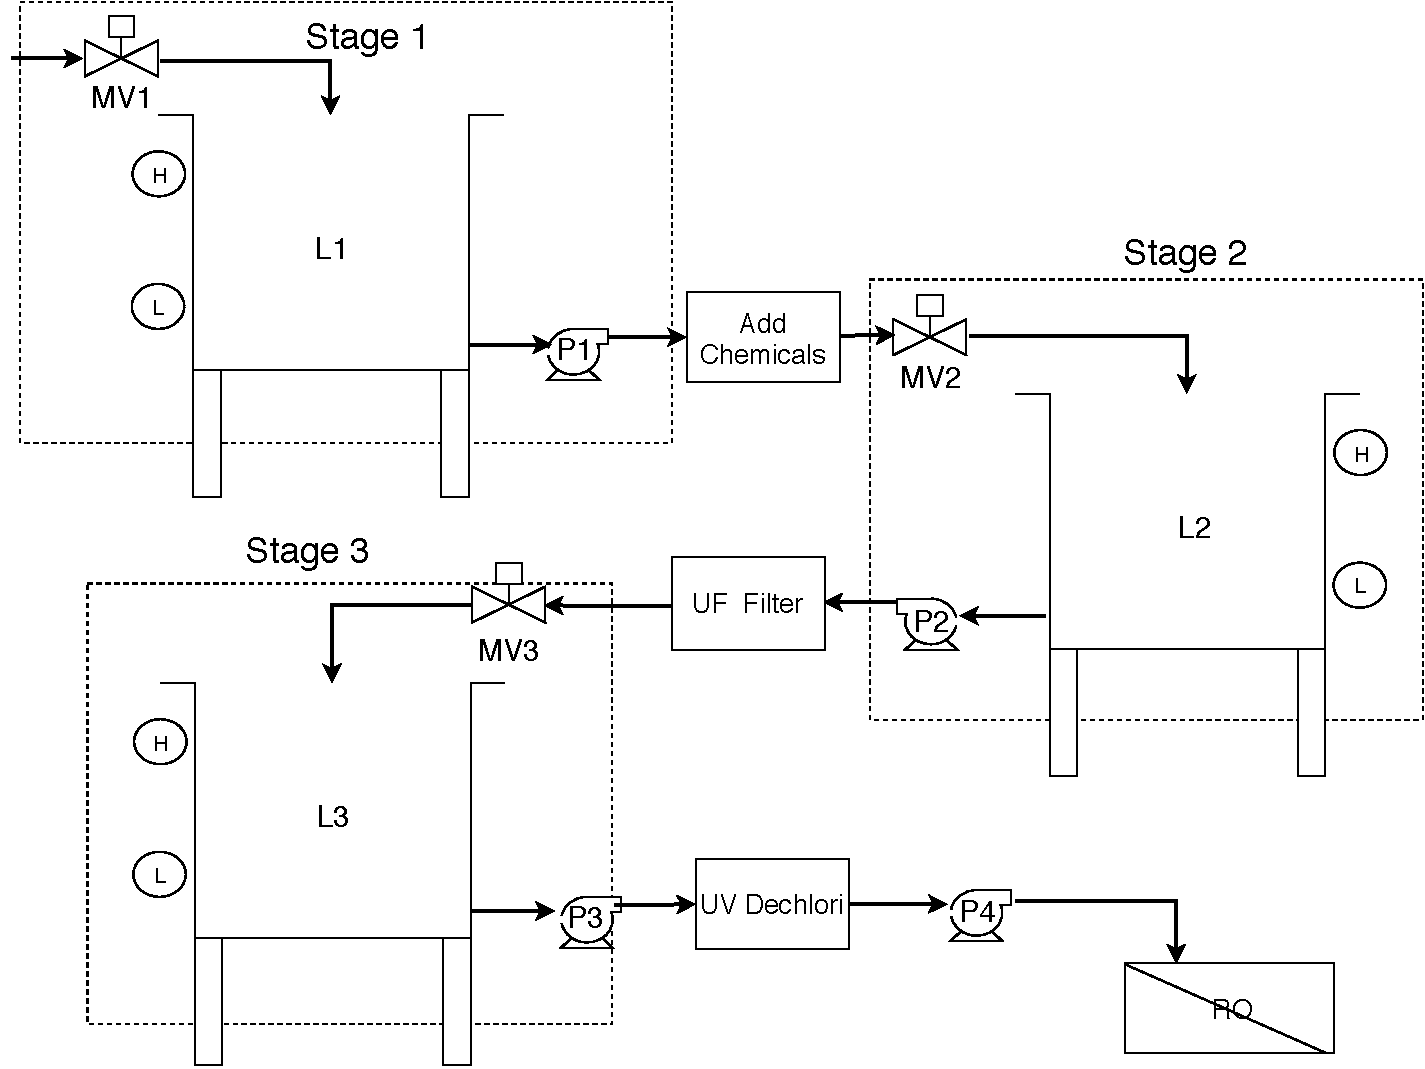
\includegraphics[width=\linewidth]{Figures/SWaT_allTanks-Stages}
  \end{subfigure}
  %
  \begin{subfigure}[b]{.35\linewidth}
  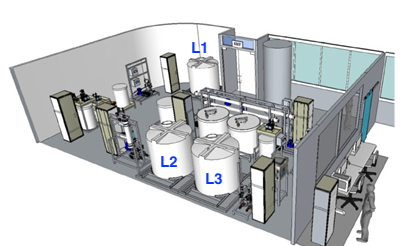
\includegraphics[width=\linewidth]{Figures/testbed.png}
  \end{subfigure}
  %
  \begin{subfigure}[b]{.35\linewidth}
  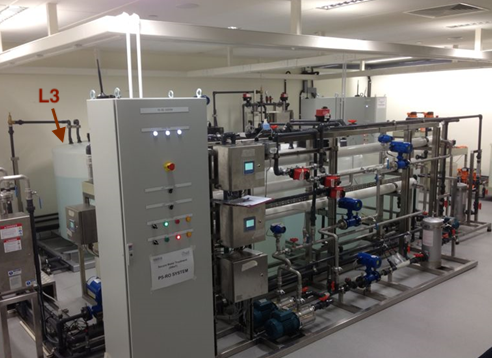
\includegraphics[width=\linewidth]{Figures/testbed2.png}
  \end{subfigure}
  
    \caption{SWaT diagram}
  \label{fig:CPSRobustness:SWaTSchema}
\end{figure}

%==================END JOHN WORKSPACE====================
%==================BEGIN ERIC WORKSPACE====================
\subsection{SWaT Stage 3}
Recall the motivational example presented in Section~\ref{sec:CPSRobustness:example} that models a water tank; such water tank is the Stage 3 submodule of SWaT. We reuse the dynamics presented in Section~\ref{sec:CPSRobustness:example} (which we henceforth refer to as Stage 3), but since there are also pumps and valves in the other process we model, i.e., Stage 2, we rename the components: $MV$, $L$, and $P$ from Section~\ref{sec:CPSRobustness:example} are now respectively $MV3$, $L3$ and $P3$, matching the descriptions in Figure~\ref{fig:CPSRobustness:SWaTSchema}.

Stage 3 receives water from Stage 2, and the controller of Stage 3 reports to the controller of Stage 2 the following information: the level of water in the tank $T3$ and the state of the valve $MV3$. To model the composition of Stage 3 with Stage 2, we define the behaviour of the communication channels $\vec{a}$, and $\vec{w}$ for Stage 2, and $\vec{b}$ and $\vec{v}$ for Stage 3. Let  
\begin{align}
  \vec{b}[L3](k+1)&\triangleq \vec{q}[L3](k)\\
  \vec{b}[MV3](k+1)&\triangleq \vec{q}[MV3](k)\\
  \vec{w}[L2](k)&\triangleq \vec{v}[L2](k),\\
  Inflow(k)&=\begin{cases}
    0 & \quad \text{if $\vec{w}[L2](k)=0$}\\
    0.31,&\quad \text{if $\vec{x}[MV](k)=\texttt{open}$}\\
    0,&\quad \text{if $\vec{x}[MV](k)=\texttt{closed}$}\\
    0.26,&\quad \text{otherwise}\\
  \end{cases}
\end{align}
where $\vec{v}[L2](k)$ is part of the behaviour description of Stage 2. The inflow of water for $T3$ now depends on the physical state of $T2$; if there is no water in $T2$, there is no inflow.

We now formally model Stage 2 and describe its composition with Stage 3. We then characterise an attacker model to measure the robustness of the composition, which we then proceed to redesign and prove that its robustness improves with respect to given the attacker model.

\subsection{A Formal Model of Stage 2}
We provide a model of SWaT Stage 2. This model has three physical components $MV2$, $L2$ and $P2$, and uses the constants $L2min=800$, $L2max=1000$ and $T2=7$.

\paragraph{The Controller $\plc_2$.} 
This controller has eight modes which depend on the state of the pump $P2$ and the valve $MV2$, and a timer, so $\vec{q}$ has three coordinates: $P2$, $MV2$, and $\tau2$. Their respective ranges are 
\begin{align*}
  \vec{q}[P2]&\in\set{\texttt{off},\texttt{on}},\\
  \vec{q}[MV2]&\in\set{\texttt{closed},\texttt{opening},\texttt{open},\texttt{closing}},\\
  \vec{q}[\tau2]&\in\mathbb{N}
\end{align*}

The controller $\plc_2$ receives a network input $\vec{a}$ and a sensor reading $\vec{y}$, and produces a control command $\vec{u}$. Through this section, we assume that every actuator and sensor behaves like a faithful single state transducer, i.e. $\vec{i}(k)=\theta_{\vec{Y}}(\vec{y}(k))=\vec{y}(k)$ and $\vec{u}(k)=\theta_{\vec{O}}(\vec{o}(k))=\vec{o}(k)$. 
The network input $\vec{a}$ has two coordinates $L3$ and $MV3$, whose ranges are 
\begin{align*}
  \vec{a}[L3]&\in[0..1200],\\ 
  \vec{a}[MV]&\in \{\texttt{closed},\texttt{opening},\texttt{open},\texttt{closing}\}.
\end{align*} 
The sensor reading $\vec{y}$ has one coordinate $L2$, where $\vec{y}[L2]\in[0..1200]$. 
The control command $\vec{u}$ has two coordinates, $MV2$ and $L2$, where 
\begin{align*}
  \vec{u}[P2]&\in\set{\const_\texttt{off},\const_\texttt{on},\id},\\
  \vec{u}[MV2]&\in\set{\texttt{closed},\texttt{opening},\const_\texttt{open},\const_\texttt{closing}, \id}.
\end{align*}
%$\vec{u}[MV2]\in\set{\const_\texttt{closed},\const_\texttt{opening},\const_\texttt{open},\const_\texttt{closing}}$.

Let $L3_k=\vec{a}[L3](k)$, $MV3_k=\vec{a}[MV3](k)$, $MV2_k=\vec{q}[MV2](k)$, $P2_k=\vec{q}[P2](k)$, and $L2_k=\vec{y}[L2](k)$; we define the behaviour of the controller PLC2 as follows:
%The controller has the function $\delta_{\vec{Q}}$, defined by
\begin{align}
  % \delta_{\vec{Q}}&((P2,MV2,\tau_2),(L,MV),L2)\triangleq (P2', MV2',\tau_2'),\text{where}\\
\vec{q}[P2](k+1)&\triangleq
    \begin{cases}
      \texttt{off},&\quad \text{if $L3_k\leq L3min$ or $MV3_k\in \set{\texttt{closed},\texttt{closing}}$},\\
      \texttt{on},&\quad \text{if $L3_k \geq L3min$ or $MV3_k\in \set{\texttt{open},\texttt{opening}}$}\\
      P2_k&\quad \text{otherwise;}
    \end{cases}\\
\vec{q}[MV2](k+1)&\triangleq
  \begin{cases}
    \texttt{opening},&\quad \text{if $MV2_k=\texttt{closed}$ and $L2_k\leq L2min$,}\\
    \texttt{open},&\quad \text{if $MV2_k=\texttt{opening}$ and $\tau2_k>T_2$,}\\
    \texttt{closing},&\quad \text{if $MV2_k=\texttt{open}$ and $L2_k\geq L2max$,}\\
    \texttt{closed},&\quad \text{if $MV2_k=\texttt{closing}$ and $\tau2_k>T_2$,}\\
    MV2&\quad \text{otherwise;}    
  \end{cases}\\
\vec{q}[\tau2](k+1)&\triangleq
\begin{cases}
  \tau2_k+1 &\quad \text{if $MV2_k\in \set{\texttt{opening},\texttt{closing}}$}\\
  0&\quad \text{otherwise;}    
\end{cases}\\
\vec{u}[MV2](k+1)=&\const_{MV2_k},\\%\vec{q}[MV2](k)\\%
\vec{u}[P2](k+1)=&\const_{P2_k}.%\vec{q}[P2](k)\\%
\end{align}
% \begin{align*}
%   \theta_{\vec{Q}}(P2,MV2,t)&\triangleq (\vec{o}[MV2],\vec{o}[P2]), \text{where}\\
%   \vec{o}[MV2]&\triangleq MV2
%     % \begin{cases}
%     %   \texttt{open},&\quad  \text{if $MV2=\texttt{opening}$}\\
%     %   \texttt{close},&\quad\text{if $MV2=\texttt{closing}$}\\  
%     %   \perp,&\quad\text{otherwise;}   
%     % \end{cases},
%   ,\quad \text{and }\quad
%   \vec{o}[P2]\triangleq P2
%   % \begin{cases}
%   %   \texttt{on}(),&\quad  \text{if $P2=\texttt{on}$}\\
%   %   \texttt{off}(),&\quad\text{if $P2=\texttt{off}$}\\  
%   %   \perp,&\quad\text{otherwise;}   
%   % \end{cases}
%   \\ 
%   \beta_{\vec{Q}}(P2,MV2,t) &\triangleq \perp.
% \end{align*}
% \paragraph{The Actuators} We have two actuators, the pump $P2$ and the motor valve $MV2$. Their  behaviour is modelled by the function $\theta_{\vec{O}}$, defined for $\vec{o}=(MV2,P2)$ by
% \begin{align}
%   \theta_{\vec{O}}(MV2,P2)&\triangleq (\vec{u}[MV2],\vec{u}[P2]), \text{where}\\
%   \vec{u}[MV2]&\triangleq 
%     \begin{cases}
%       \const_{MV2},&\quad  \text{if $MV2\neq\perp$,}\\
%       \id,&\quad\text{otherwise;}   
%     \end{cases},\\
%   \vec{o}[P2]&\triangleq 
%   \begin{cases}
%     \const_{P2},&\quad  \text{if $P2\neq \perp$,}\\
%     \id,&\quad\text{otherwise;}   
%   \end{cases},
% \end{align}

\paragraph{The Process} 
The state of the process $\vec{x}$ has three coordinates: $L2, MV2$ and $P2$. Their respective ranges are $\vec{x}[L2]\in [0..1200]$, $\vec{x}[MV2]\in \{\texttt{closed},\texttt{opening},\texttt{open},\texttt{closing}\}$ and $\vec{x}[P2]\in \set{\texttt{on},\texttt{off}}$. 
% subcomponents $\vec{x}=(L2,MV2,P2)$, with $\range(\vec{x}[L2])=[0..1200]$, $\range(\vec{x}[MV2])=\set{\texttt{closed},\texttt{opening},\texttt{open},\texttt{closing}}$, and $\range(\vec{x}[P2])=\set{\texttt{on},\texttt{off}}$. 

We leave the initial condition abstract for now. The behaviour of the process is given by
% \todo[inline]{@Eric:The initial state of the process is $\vec{x_0}=(990,\texttt{open},\texttt{on})$.}
%The process reacts to the control input $\vec{u}$,

% The process has the function $\delta_{\vec{X}}$, which computes the of value of $\vec{x}(k+1)$ from $\vec{x}(k)$, $\vec{u}[MV2](k)$ and $\vec{u}[P2](k)$
Let $P2_k=\vec{x}[P2](k)$, $MV2_k=\vec{x}[MV2](k)$, and $L2_k=\vec{x}[L2](k)$, and let $\delta_{P2}=\vec{u}[P2](k)$, and $\delta_{MV2}=\vec{u}[MV2](k)$; we define the behaviour of the process by
\begin{align*}
  %\delta_{\vec{X}}&((L2,MV2,P2),(\vec{u}[MV2],\vec{u}[P2]))\triangleq (L2', MV2',P2'),\text{where}\\
\vec{x}[P2](k+1)&\triangleq \delta_{P2}(P2_k)\\
\vec{x}[MV2](k+1)&\triangleq \delta_{MV2}(MV2_k)\\
\vec{x}[L2](k+1)&\triangleq L2_k+\partial(MV2_k,P2_k),\text{where}\\
\partial(MV2,P2)&\triangleq
\begin{cases}
  0&\quad \text{if $MV2_k=\texttt{closed}$ and $P2_k=\texttt{off}$}\\
  0.46&\quad \text{if $MV2_k=\texttt{open}$ and $P2_k=\texttt{off}$}\\
  0.29&\quad \text{if $MV2_k\in\set{\texttt{opening},\texttt{closing}}$ and $P2_k=\texttt{off}$}\\
  -0.29&\quad \text{if $MV2_k=\texttt{closed}$ and $P2_k=\texttt{on}$}\\
  0.13&\quad \text{if $MV2_k=\texttt{open}$ and $P2_k=\texttt{on}$}\\
  -0.28&\quad \text{if $MV2_k\in\set{\texttt{opening},\texttt{closing}}$ and $P2_k=\texttt{on}$}\\  
\end{cases}
\end{align*}
The values for $\partial(MV2,P2)$ were computed by linear regression to approximate the flow equation $L2_{k+1}=L2_{k}+\texttt{Inflow}_k-\texttt{Outflow}_k$.

The sensor reading $\vec{y}$ has only one coordinate $L2$, whose range is $\vec{y}\in \mathbb{R}^+$; i.e, any positive value. The behaviour of $\vec{y}$ is given by 
\begin{align}
  \vec{y}[L2](k)=\vec{x}[L2]
\end{align}

Finally, the physical state of the process propagates to Stage 3 via the abstract channel $\vec{v}[L3]$
\begin{align}
  \vec{v}[L2](k)&\triangleq \vec{x}[L2](k)
\end{align}
Figure~\ref{fig:CPSRobustness:Stage2Normal} shows the normal steady state behaviour of the water level in tank T2. Due to interdependence, many changes in the behaviour of the tank T2 affect the behaviour of tank T3 and vice versa. 
%\todo[inline]{@John: we are doing testing so it should be fine, but I can imagine a reviewer complaining about the omision of the error parameter. What reasoning can we use to omit explicitly including the error parameter?}

% \todo[inline]{@All. Reviewers might ask why we do not include errors in the models. They can be added, but I wanted to keep the model as simple as possible.}

% The process produces the output $\theta_{\vec{X}}$, defined by
% \begin{align*}
%   \theta_{\vec{X}}(\vec{x})\triangleq \vec{y}[L2], \text{where $\vec{y}[L2]=\vec{x}[L2]$}.
% \end{align*} 
% \paragraph{Sensors} Finally, the behaviour of the water level sensor is given by the function $\theta_{\vec{Y}}$, defined by 
% \begin{align*}
%   \theta_{\vec{Y}}(\vec{y})\triangleq \vec{i}[L2]\text{, where $\vec{i}[L2]=\vec{y}[L2]$.}
% \end{align*}

\begin{figure}[t]
  \centering
  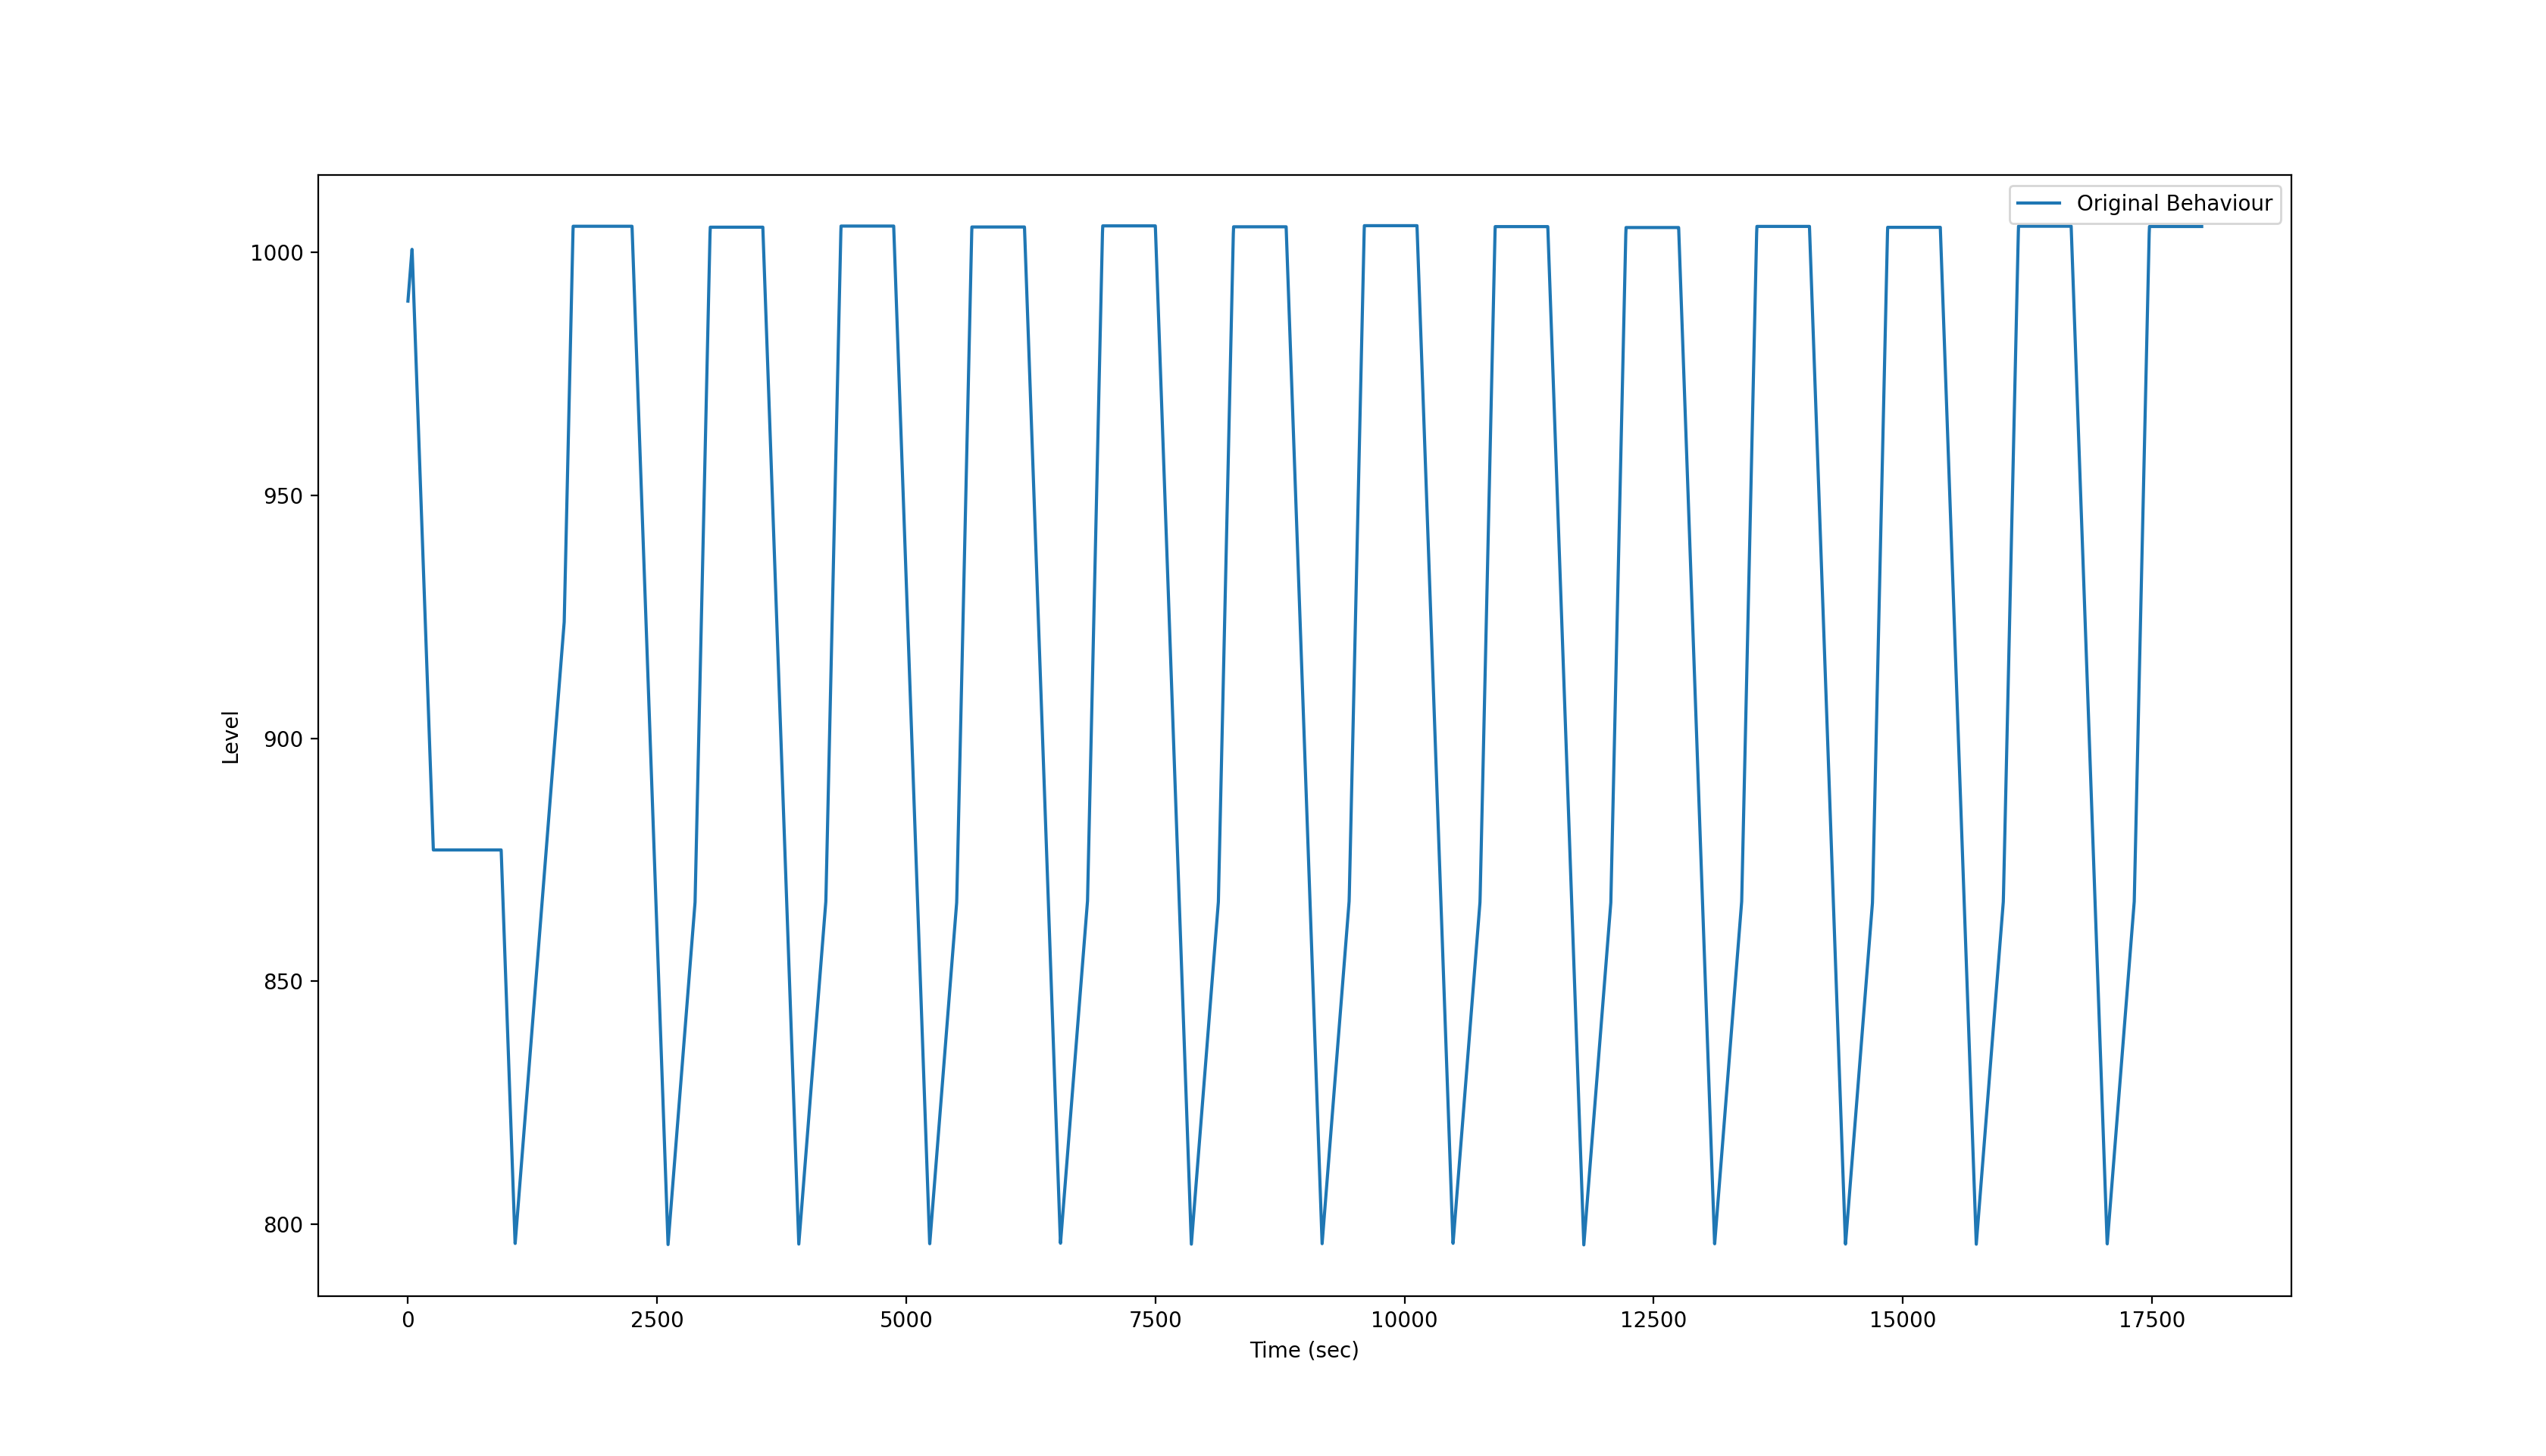
\includegraphics[width=0.75\textwidth]{Figures/Stage2Normal.png}
  \caption{Normal behaviour of the water level of Stage 2 if Stage 3 is also operating normally.}
  \label{fig:CPSRobustness:Stage2Normal}
\end{figure}

% The controller has the output functions $\beta_{\vec{Q}}$ and $\theta_{\vec{Q}}$, defined by
% \begin{align}
%   \theta_{\vec{Q}}(P2,MV2,t)&\triangleq (\vec{o}[MV2],\vec{o}[P2]), \text{where}\\
%   \vec{o}[MV2]&\triangleq 
%     \begin{cases}
%       \texttt{open}(),&\quad  \text{if $MV2=\texttt{opening}$}\\
%       \texttt{close}(),&\quad\text{if $MV2=\texttt{closing}$}\\  
%       \perp,&\quad\text{otherwise;}   
%     \end{cases},\\
%   \vec{o}[P2]&\triangleq P2\\ 
%   \beta_{\vec{Q}}(P2,MV2,t) &\triangleq \perp.
% \end{align}

\subsection{Attacker Model}%{Some Attacker Models of Stage 2 and Stage 3}
% We define an attacker model for the composition of Stage 2 and Stage 3 by combining two attacker models, one for Stage 2 and one for Stage 3.  The following models describe single-point attackers in one of the processes.
We now define an attacker model using Definitions~\ref{def:CPSRobustness:AttackBasis}, \ref{def:CPSRobustness:IdempotentMonoid}, and~\ref{def:CPSRobustness:Attack} for the quantification of robustness. We have four security requirements: $\Always{\vec{x}[L2]>0}$, $\Always{\vec{x}[L2]<1200}$, $\Always{\vec{x}[L3]>0}$ and $\Always{\vec{x}[L3]<1200}$. 
We consider an attacker model that manipulates the control outputs of the controller PLC2 for pump $P2$ and valve $MV2$. We choose this attacker because they can override the commands sent by PLC2, giving them the same level of control than the PLC2. For testing, we allow this attacker to set $\vec{u}[MV2](k)$ and $\vec{u}[P2](k)$ for all $0\leq k\leq t$ given some testing time parameter $t$, which we set to 6 hours to give the effect of actions of the attacker enough time to propagate through the system. To define the attacker model, we reuse the base from Example~\ref{ex:CPSRobustness:AttackBasis}. The base for the attacker model is $[LL, OK, HH]^T$, where ${LL}(\pi)=\pi[\vec{x}[L3]]<L3min$, ${HH}(\pi)=\pi[\vec{x}[L3]]>L3max$ and ${OK}(\pi)=L3min \leq \pi[\vec{x}[L3]]\leq L3max$, for $\pi \in \Pi$. This implies that even though the attacker modifies components in Stage2, they only have visibility of the tank T3 and not of T2. Although this attacker is ``blind" with respect to $T2$, their actions will definitely impact the behaviour of $T2$. The representative values used by the attacker model for $\vec{u}[MV2]$ are $\texttt{open}$ and $\texttt{closed}$; more precisely, we define
\begin{align*}
  \Gamma_{\vec{u}[MV2]}=\set{\const^{\vec{u}[MV2]}_{\texttt{open}}, \const^{\vec{u}[MV2]}_{\texttt{closed}}}.
\end{align*}
The representative values for $\vec{u}[P2]$ are $\texttt{on}$ and $\texttt{off}$, which create the constant functions
\begin{align*}
  \Gamma_{\vec{u}[P2]}=\set{\const^{\vec{u}[P2]}_{\texttt{on}}, \const^{\vec{u}[P2]}_{\texttt{off}}}.
\end{align*}
% The set of coefficients for this attacker model is $\Gamma_{\vec{u}[MV2],\vec{u}[P2]}=\Gamma_{\vec{u}[MV2]}\cup \Gamma_{\vec{u}[P2]}$. 
The attacks of this attacker model $\vec{m}$ are then of the form
\begin{align*}
  \vec{m}(\pi)=
  %[t_1,\ldots,t_n]
  \begin{bmatrix}
    t_{LL}\circ s_{LL} \\
    t_{OK}\circ s_{OK} \\
    t_{HH}\circ s_{HH} \\
  \end{bmatrix}
  \cdot
  \begin{bmatrix}
    LL \\
    OK \\
    HH
  \end{bmatrix},
\end{align*} 
where $t_i\in \set{\id,\const^{\vec{u}[MV2]}_{\texttt{open}}, \const^{\vec{u}[MV2]}_{\texttt{closed}}}$ and  $s_i\in\set{\id,\const^{\vec{u}[P2]}_{\texttt{on}}, \const^{\vec{u}[P2]}_{\texttt{off}}}$, for $i\in \set{LL,OK,HH}$. The resulting attacker model has 729 attacks because
 \begin{align*}
  \left| \IM{\Gamma_{\set{\vec{u}[MV2],\vec{u}[P2]}}}\right|^{\left|\set{{LL},{OK},{HH}}\right|}=9^3=729.
\end{align*}

\subsection{Counterattacker Model}
The corresponding counterattacker model uses the controller PLC3; i.e. the counterattacker can set $\vec{q}[MV3](k)$ and $\vec{q}[P3](k)$ for all $0\leq k\leq t$ , with  $t=6$ hours to let the actions of the attacker and counterattacker enough time to stabilise. Since the counterattacker is in the controller of Stage 3, we define the base for the counterattacker model to be $[LL', OK', HH']^T$, where ${LL'}(\pi)=\pi[\vec{y}[L3]]<L3min$, ${HH'}(\pi)=\pi[\vec{y}[L3]]>L3max$ and ${OK'}(\pi)=L3min \leq \pi[\vec{y}[L3]]\leq L3max$, for $\pi \in \Pi$ (unlike the base of the attacker, which uses $\vec{x}[L3]$ instead of $\vec{y}[L3]$). The counterattacker is also ``blind" with respect to $T2$, but their actions also impact the behaviour of $T2$. 

We set the representative values of $\vec{q}[MV3]$ to be $\texttt{open}$, and $\texttt{closed}$ and the representative values of $\vec{q}[P3]$ to be $\texttt{on}$, and $\texttt{off}$; more precisely, 
\begin{align*}
  \Gamma_{\vec{q}[MV3]}&=\set{\const^{\vec{q}[MV3]}_{\texttt{open}}, \const^{\vec{q}[MV3]}_{\texttt{closed}}}.\\
  \Gamma_{\vec{q}[P3]}&=\set{\const^{\vec{q}[P3]}_{\texttt{on}}, \const^{\vec{q}[P3]}_{\texttt{off}}}.
\end{align*}
% The set of coefficients for this attacker model is $\Gamma_{\vec{u}[MV2],\vec{u}[P2]}=\Gamma_{\vec{u}[MV2]}\cup \Gamma_{\vec{u}[P2]}$. 
The counterattacks of this model $\vec{w}$ are then of the form
\begin{align*}
  \vec{w}(\pi)=
  %[t_1,\ldots,t_n]
  \begin{bmatrix}
    t_{LL'}\circ s_{LL'} \\
    t_{OK'}\circ s_{OK'} \\
    t_{HH'}\circ s_{HH'} \\
  \end{bmatrix}
  \cdot
  \begin{bmatrix}
    LL' \\
    OK' \\
    HH'
  \end{bmatrix},
\end{align*} 
where $t_i\in \set{\id,\const^{\vec{q}[MV3]}_{\texttt{open}}, \const^{\vec{q}[MV3]}_{\texttt{closed}}}$ and  $s_i\in\set{\id,\const^{\vec{u}[P3]}_{\texttt{on}}, \const^{\vec{u}[P3]}_{\texttt{off}}}$, for $i\in \set{LL',OK',LL'}$. This counterattacker model has 729 counterattacks.

% \begin{figure}[t]
%   \includegraphics[width=0.75\textwidth]{Figures/CounterAtkRank.pdf} 
%   \caption{Counterattack ranking}
%   \label{fig:CPSRobustness:CounterAtkRanking}
% \end{figure}


\subsection{Quantification of Robustness: Analysis of Results}
Using LBA, we quantify the robustness of the system given the initial conditions $\vec{x}[L2]=990$, $\vec{x}[MV2]=open$, $\vec{x}[P2]=on$, $\vec{x}[L3]=920$, $\vec{x}[MV3]=open$, $\vec{x}[P3]=on$. The robustness factor of 162/729, meaning that are successful 567 attacks for the given attacker model. All attacks that break $\Always{\vec{x}[L3]>0}$ or $\Always{\vec{x}[L3]<1200}$ can always be countered. However, 136 attacks cannot be countered by the proposed counterattacker model, meaning that the latent robustness of the system is only $593/729$. Non countered attacks always break either $\Always{\vec{x}[L2]>0}$ or $\Always{\vec{x}[L2]<1200}$. Nevertheless, some attacks which break $\Always{\vec{x}[L2]>0}$ or $\Always{\vec{x}[L2]<1200}$ can be countered. For example, the attack
\begin{align*}
%   Requirement "Tank T2 Never Overflows" broken at time 644 by attack (x[L3]<L3min)=>[(O[P2]->off), (O[MV2]->open)] + (L3min<=x[L3]<=L3max)=>[id(O[P2]), id(O[MV2])] + (x[L3]>L3max)=>[id(O[P2]), id(O[MV2])]
% Found counterattack(Y[L3]>L3max)=>[id(Q[MV3]), (Q[P3]->off)] + (L3min<=Y[L3]<=L3max)=>[id(Q[MV3]), id(Q[P3])] + (Y[L3]<L3min)=>[id(Q[MV3]), id(Q[P3])]
  \vec{m}(\pi)&=
  %[t_1,\ldots,t_n]
  \begin{bmatrix}
   \const^{\vec{u}[MV2]}_{\texttt{open}}\circ \const^{\vec{u}[P2]}_{\texttt{off}} \\
   \id\circ \id \\
   \id\circ \id \\
  \end{bmatrix}
  \cdot
  \begin{bmatrix}
    \pi[\vec{x}[L3]]<L3min \\
    L3min \leq \pi[\vec{x}[L3]]\leq L3max \\
    \pi[\vec{x}[L3]]>L3max
  \end{bmatrix},
\end{align*} 
breaks the requirement $\Always{\vec{x}[L2]<1200}$, but it is countered by the counterattack 
\begin{align*}
  \vec{w}(\pi)&=
  %[t_1,\ldots,t_n]
  \begin{bmatrix}
    \id\circ \id \\
    \id\circ \id \\
    \id\circ \const^{\vec{q}[P3]}_{\texttt{off}} \\
  \end{bmatrix}
  \cdot
  \begin{bmatrix}
    \pi[\vec{y}[L3]]<L3min \\
    L3min \leq \pi[\vec{y}[L3]]\leq L3max \\
    \pi[\vec{y}[L3]]>L3max
  \end{bmatrix}.
\end{align*} 
The counterattack works by preventing the conditions that trigger the attack; more precisely, the attack activates when $\pi[\vec{x}[L3]]<L3min$, and the counterattack $\vec{w}$ prevents such condition from happening (although the behaviour eventually causes the system to reach a state where water does not flow in or out of the tanks). 

The following attack
\begin{align*}
  %(x[L3]<L3min)=>[id(O[P2]), id(O[MV2])] + (L3min<=x[L3]<=L3max)=>[(O[P2]->off), (O[MV2]->open)] + (x[L3]>L3max)=>[(O[P2]->off), id(O[MV2])]
    \vec{m}'(\pi)&=
    %[t_1,\ldots,t_n]
    \begin{bmatrix}
     \id\circ \id \\
     \const^{\vec{u}[MV2]}_{\texttt{open}}\circ \const^{\vec{u}[P2]}_{\texttt{off}} \\
     \id\circ \const^{\vec{u}[P2]}_{\texttt{off}} \\
    \end{bmatrix}
    \cdot
    \begin{bmatrix}
      \pi[\vec{x}[L3]]<L3min \\
      L3min \leq \pi[\vec{x}[L3]]\leq L3max \\
      \pi[\vec{x}[L3]]>L3max
    \end{bmatrix}
  \end{align*} 
causes tank T2 to overflow, and it cannot be countered using the current counterattacker model. This and similar attacks cannot be countered because the controller of Stage 3 cannot compensate the effects of an attacker controlling $\vec{u}[MV2]$ by influencing other components. 

\subsection{Increasing Robustness}
%\todo[inline]{Discuss a couple of attack and counterattack dynamics, several counterattacks vs several attacks with some things in common.}
Using LBA, we can group attacks that are countered by the same counterattack. After evaluating the composition of Stage 2 and Stage 3 under the given attacker and counterattacker models, we observe 12 counterattacks to address 431 successful attacks. The number of attacks countered by each counterattack does not follow a uniform distribution; some counterattacks counter only a couple of attacks, while others counter hundreds. 

For a given counterattack $\vec{w}$ which counters $n$ attacks $\vec{m}_1, \ldots, \vec{m}_n$, understanding the similarities among the $n$ attacks gives us a good indication of the reason why the counterattack is effective. For this evaluation, we manually analysed possible common causes, but a more systematic and efficient methodology is encouraged for future work. In summary, we identified 333 attacks that cause T2 to overflow, 126 that cause T2 to empty and 108 that cause T3 to empty; no attack caused T3 to overflow because we stop analysis at the first cause of problem, and attacks that can overflow T3 can also overflow T2, empty T2 or empty T3 faster than they can overflow T3.


\subsubsection{A Correct Repair}
\label{sec:CPSRobustness:CorrectRepair}
For an attack $\vec{m}$ and a counterattack $\vec{w}$ which counters it, if we implement the composition $\vec{w}\circ \vec{m}$, this transformation does not break the requirements of the system, although it may take the system to exceptional states. In general, implementing the application of a counterattack is far from trivial: the counterattack must only be applied when an attack it counters is detected; otherwise, the counterattack itself may become an attack! 

In Section~\ref{sec:CPSRobustness:UrgentAttacker}, we mentioned that to implement a counterattack, we must ensure that it is only applied when the attack it counters exists in the system. This implicitly assumes the existence of a system monitor that can correctly identify which attack is being applied to the system; i.e., it properly identifies $\vec{m}$. Once $\vec{m}$ is identified, the monitor applies the appropriate counterattack for $\vec{m}$. Given that this requitements over the monitor are quite restrictive, we explore in the following a different approach: we directly modify the program of a controller PLC, and we run LBA to measure the robustness of the new system to check if it improved. 

We used a counterattacker model which acts on the coordinates $\vec{q}[MV3]$ and $\vec{q}[P3]$ which are normally controlled by controller PLC3. Our plan then is to incorporate a counterattack $\vec{w}$ as part of the program of PLC3. Two parts are necessary: the conditions that would trigger the application of the counterattack, and the right effects over $\vec{q}[MV3]$ and $\vec{q}[P3]$. We observe that several attacks that empty tank T3 can be countered by means of the counterattack 
\begin{align*}
  %(Y[L3]>L3max)=>[id(Q[MV3]), (Q[P3]->off)] + (L3min<=Y[L3]<=L3max)=>[id(Q[MV3]), id(Q[P3])] + (Y[L3]<L3min)=>[id(Q[MV3]), id(Q[P3])]
    \vec{w}(\pi)&=
    %[t_1,\ldots,t_n]
    \begin{bmatrix}
    \id\circ \const^{\vec{q}[P3]}_{\texttt{off}} \\
     \id\circ \id \\
     \id\circ \id \\
    \end{bmatrix}
    \cdot
    \begin{bmatrix}
      \pi[\vec{y}[L3]]<L3min \\
      L3min \leq \pi[\vec{y}[L3]]\leq L3max \\
      \pi[\vec{y}[L3]]>L3max
    \end{bmatrix},
  \end{align*} 
which is sensible: if the tank $T3$ is losing water, by shutting off the pump $P3$ when the level is low, we prevent water from leaving the tank. The counterattack $\vec{w}$ counters 122 attacks in total.

The counterattack $\vec{w}$ defines the effects over $\vec{q}[MV3]$ and $\vec{q}[P3]$ to be triggered by the controller PLC3: do nothing with respect to $\vec{q}[MV3]$ and set $\vec{q}[P3]$ to $\texttt{off}$ only if $\pi[\vec{y}[L3]]<L3min$. We now need to establish the conditions that would trigger these effects, and for that we look at common elements among the attacks countered by $\vec{w}$. We observe among several of those attacks that they share the factor $(\const^{\vec{u}[P2]}_{\texttt{off}})(\vec{x}[L3]]<L3min)$; this provides the trigger condition for the application of the effects given by $\vec{w}$.More precisely, to implement the counterattack $\vec{w}$ as part of the controller PLC3, we change its program to set $\vec{q}[P3]$ to \texttt{off} if $\vec{u}[P2]$ is \texttt{off} and $\vec{y}[L3]]<L3min$; we use $\vec{y}[L3]]<L3min$ instead of $\vec{x}[L3]]<L3min$ because $\vec{y}[L3]=\vec{x}[L3]$, because PLC3 has access to $\vec{y}[L3]$, and because the attacker model does not include the coordinate $\vec{y}[L3]$. 

After implementing these changes, we run LBA again. We see that the changes to PLC3 increase the robustness of the system from $162/729$ to $333/729$, since the controller PLC3 now prevents the tank T3 from running out of water due to the effect of 171 previously successful attacks. We recall that $\vec{w}$ countered 122 attacks according to the original LBA, so the change to the program of PLC3 is more profound than anticipated. Nevertheless, the increase in robustness indicates that the system is now more robust after the change, even if the latent robustness remains the same, $593/729$. 

%  that broke this requirement in the original system. The latent robustness remains at 581/729, which means that implementing this counterattack did not add additional vulnerabilities.
 
\subsubsection{A Non-Repair} 
\label{sec:CPSRobustness:NonRepair} We now explore the effects of a modification to the program of PLC3 that does not improve the overall robustness of the system; i.e. a non-repair. The counterattack 
\begin{align*}
%(Y[L3]>L3max)=>[(Q[MV3]->open), id(Q[P3])] + (Y[L3]<L3min)=>[id(Q[MV3]), id(Q[P3])] + (L3min<=Y[L3]<=L3max)=>[id(Q[MV3]), id(Q[P3])] counters the following 42 attacks:
    \vec{w'}(\pi)&=
    %[t_1,\ldots,t_n]
    \begin{bmatrix}
     \id\circ \id \\
     \const^{\vec{q}[MV3]}_{\texttt{open}}\circ \id \\
     \id\circ \id \\
     %\const^{\vec{q}[MV3]}_{\texttt{open}}\circ \id
    \end{bmatrix}
    \cdot
    \begin{bmatrix}
      \pi[\vec{y}[L3]]<L3min \\
      L3min \leq \pi[\vec{y}[L3]]\leq L3max \\
      \pi[\vec{y}[L3]]>L3max
    \end{bmatrix},
  \end{align*} 
%\todo[inline]{Python keeps playing tricks: sometimes it uses this as a counterattack, sometimes it finds another. it's driving me mad.}
counters 58 attacks, many of which overflow T2 and have a common factor of $(\vec{x}[L3]>L3max)\const^{\vec{u}[P2]}_{\texttt{on}}$, i.e., many attacks turn on the pump $P2$ then the level of tank $L3$ is beyond the safety limit $L3max$. 
%\todo[inline]{@John: What happens when the pump is on and the valve is closed? Where does the water go? Reviewers might ask.}
\begin{figure}[t]
  \centering
  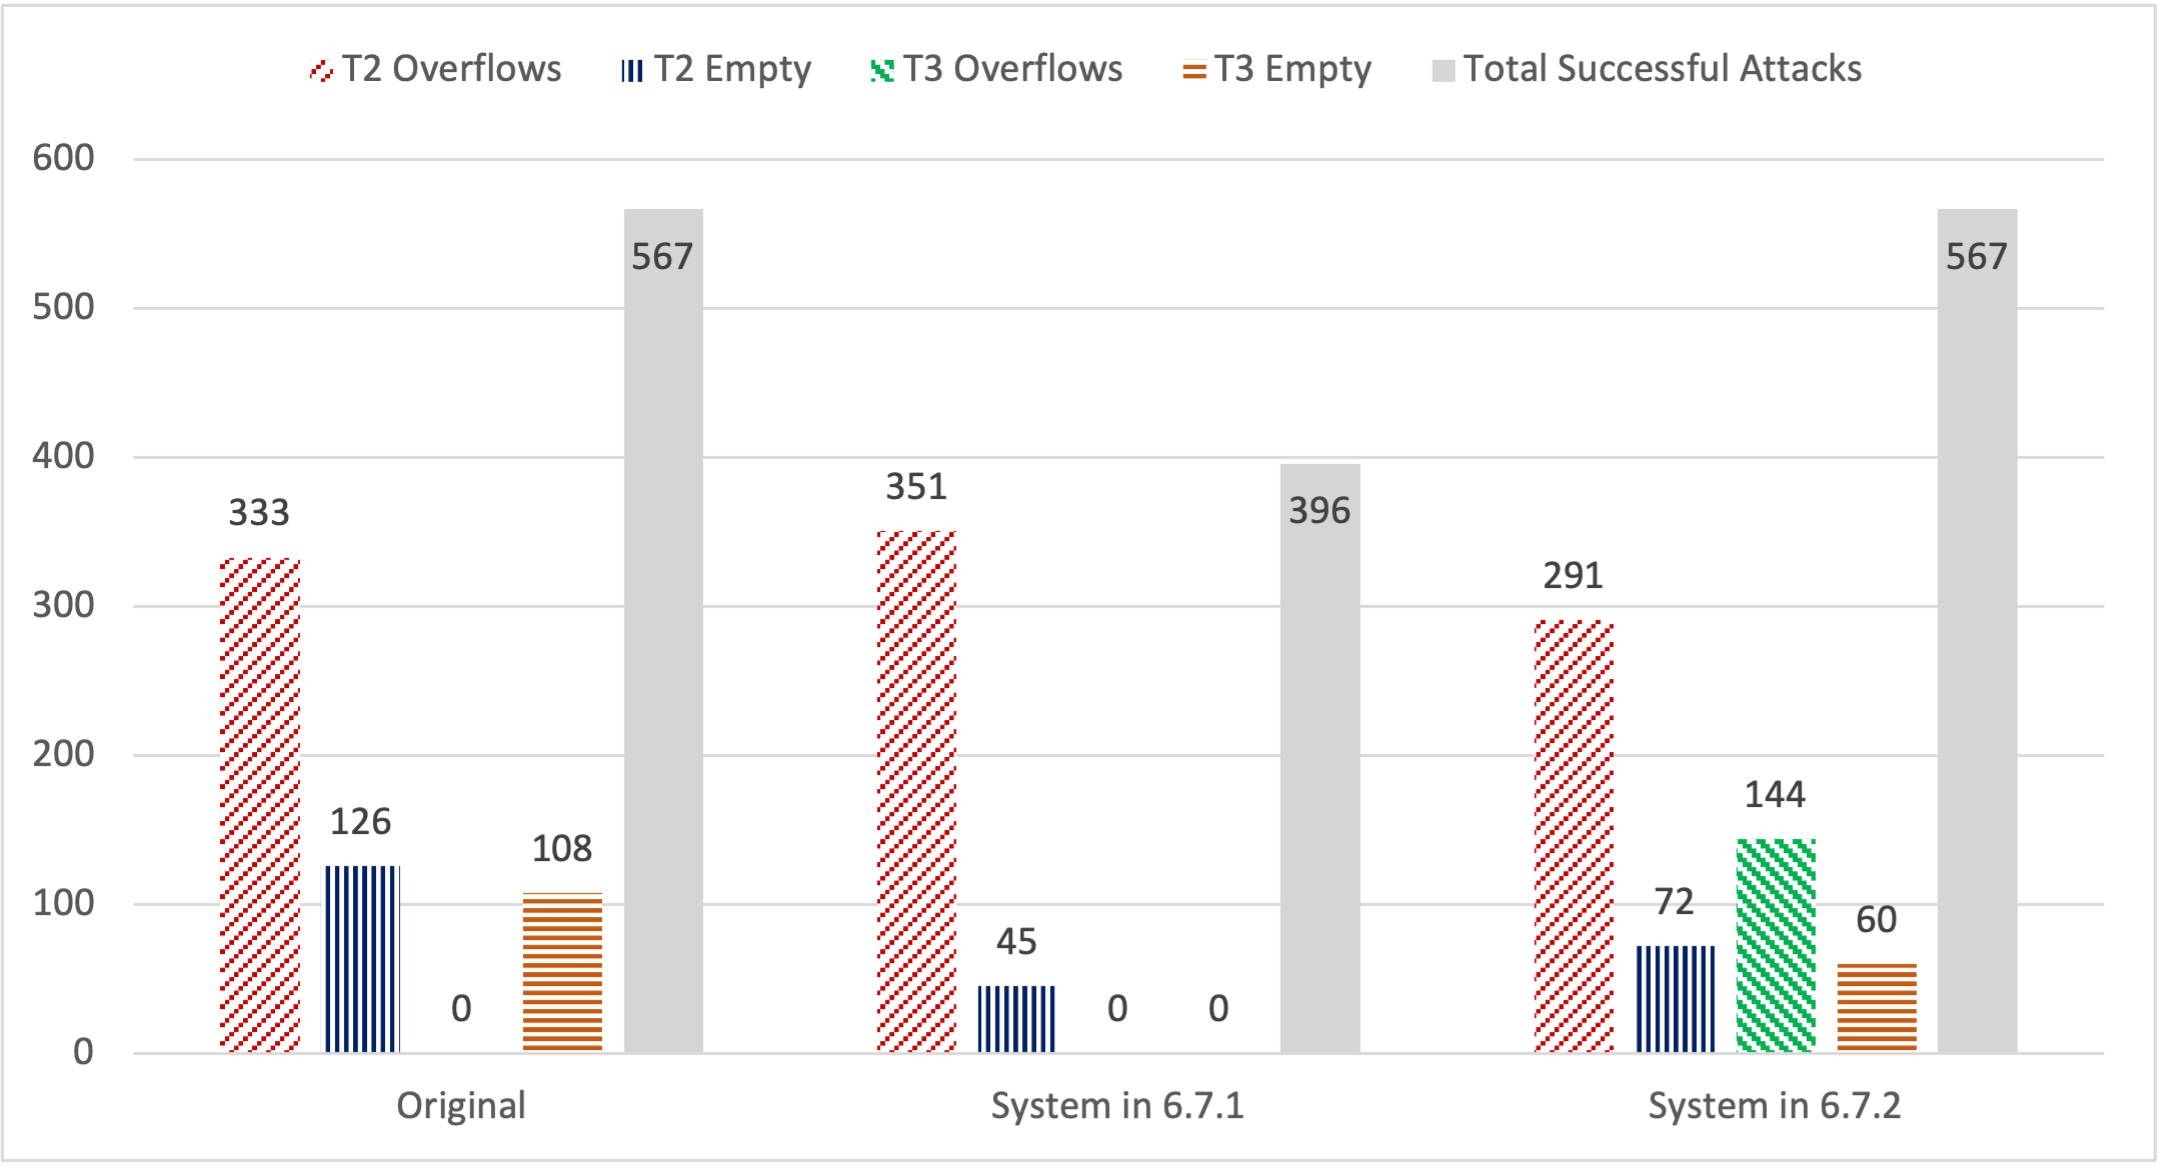
\includegraphics[width=0.75\textwidth]{Figures/AttackDistribution.png} 
  \caption{Attack distribution with respect to the first broken requirement for the original system, the repaired system from Section~\ref{sec:CPSRobustness:CorrectRepair} and the non-repaired system from Section~\ref{sec:CPSRobustness:NonRepair}}
  \label{fig:CPSRobustness:AttackDistribution}
\end{figure} 
Since the condition of the attacks $(\vec{x}[L3]>L3max)$ does not match the condition of the counterattack $L3min \leq \pi[\vec{y}[L3]]\leq L3max$, we just create a rule in the controller that implements the counterattack $\vec{w'}$. To check if such modification improved robustness, we perform LBA, and we observe that the robustness factor remains the same at 162/729; i.e., this new system can also withstand the effect of 162 attacks.  We observe two major differences: the latent robustness of the system changed from 593/729 to 606/729, and the distribution of attacks with respect to the first requirement they break also changes, as shown in Figure~\ref{fig:CPSRobustness:AttackDistribution}. The robustness of the new system is equal to the original robustness, so we cannot consider this to be an improvement over the previous version of the system, which is why we affirm this modification is an example of a non-repair. While this modification reduced the number of attacks that overflow tank T2, it now enables attacks that overflow tank T3, which were previously inexistent. More precisely, in the original system, no attack caused T3 to overflow, but now there are 144 attacks whose first broken requirement is to overflow tank T3. An increase in latent robustness indicates that more attacks in this new system can be countered. This vaguely indicates that the \emph{security potential} increased with respect to the given attacker and counterattacker model.

% Figure \ref{fig:CPSRobustness:AttackDistribution} shows the distribution of attacks for all three systems. Both the original and the non-repaired system have the same number of successful attacks, although their distribution changes.


\subsection{Discussion of Results}
We can use LBA and a testing methodology (e.g., simulation) to check if an arbitrary modification enhances the robustness of the system by comparing the resulting robustness factor. 
We propose two changes to the original Stage 2 and Stage 3 system; one is a repair since it strictly improves the robustness of the system, while the other is not since it only changes the distribution of successful attacks. We believe that a more systematic analysis of the large amounts of data obtained via LBA can produce meaningful suggestions for correct model repairs, e.g., we believe that using machine learning or clustering techniques to find common causes of attacks that are countered by the same counterattack, or finding similarities among counterattacks for the same types of requirements might help the implementation of both system monitors and repairs. 

\begin{figure}[t]
  \centering
  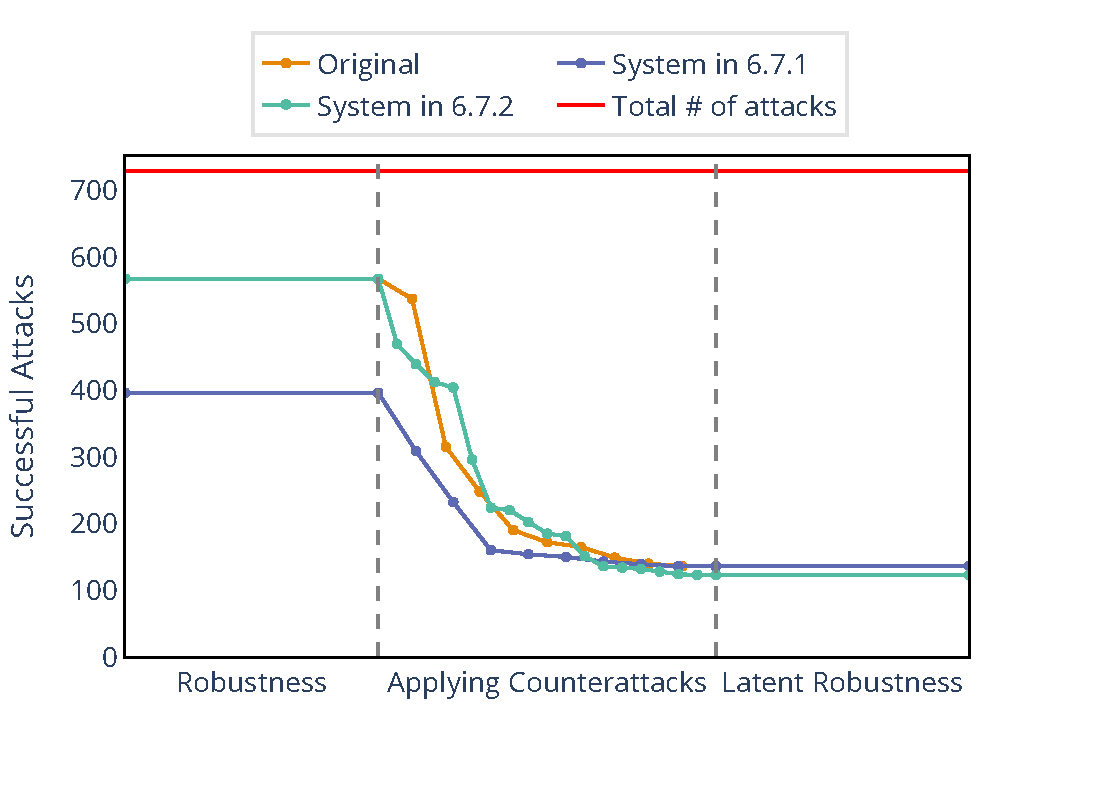
\includegraphics[width=0.75\textwidth]{Figures/Robustness.pdf} 
  \caption{Robustness improvement. The implementation of counterattacks improves the robustness of the system, making it susceptible to fewer attacks.}
  \label{fig:CPSRobustness:Robustness}
\end{figure}
Figure ~\ref{fig:CPSRobustness:Robustness} shows a transition from the robustness innate to the systems presented in this section and their latent robustness. This transition assumes that counterattacks are properly implemented, and that an adequate attack identification monitor exists. A properly implemented counterattack reduces the number of successful attacks, which in turn increases the robustness of the system. Each dot in the ``applying counterattacks'' section corresponds to the cumulative reduction of successful attacks by the proper implementation of a counterattacks that we identified using LBA. By proper implementation of counterattacks, we do not imply that we incorporate them all as part of the normal functionality of the system; instead, that they only activate when it is adequate in an exceptional reactive mode of the system. The slight difference in latent robustness is due to the fact that the original system and the system in Section~\ref{sec:CPSRobustness:NonRepair} are different, and the latter has more attacks that can be countered under the current attacker/counterattacker models. 

For this experiment, we used a very basic counting unweighted metric for robustness that assumes all requirements are equally important. We can refine the definitions of robustness and latent robustness from Definitions~\ref{def:CPSRobustness:Robustness} and \ref{def:CPSRobustness:LatentRobustness} metrics to represent a larger lack of robustness if a particular security requirement is broken by many attacks. 

%, similar to the repair presented in Section ~\ref{sec:CPSRobustness:CorrectRepair}.

% We implement the counterattack $\vec{w'}$ similarly to how we implemented $\vec{w}$: we change the program of PLC3 such that so that, under common conditions given by the countered attacks, we apply the changes indicated by the counterattack $\vec{w'}$. More precisely, PLC3 now sets $\vec{q}[MV3]$ to \texttt{open} if $\pi[\vec{y}[L3]]>L3max$, but it only responding to the factor $(\const^{\vec{u}[P2]}_{\texttt{on}})(\vec{x}[L3]]<L3min)$. Clearly, both $\vec{x}[L3]]<L3min$ and $\pi[\vec{y}[L3]]>L3max$ are mutually exclusive, so this repair does nothing. 

% (Y[L3]>L3max)=>[id(Q[MV3]), (Q[P3]->off)] + (L3min<=Y[L3]<=L3max)=>[id(Q[MV3]), id(Q[P3])] + (Y[L3]<L3min)=>[id(Q[MV3]), id(Q[P3])]
% because
%  \begin{align*}
%   \left| \IM{\Gamma_{\set{\vec{u}[MV2],\vec{u}[P2]}}}\right|^{\left|\set{{LL},{OK},{HH}}\right|}=9^3=729.
% \end{align*}

% \begin{align*}
%   \vec{m}=&(x[L3]<L3min)(\gamma_1(\vec{u}[P2]), \gamma_1(\vec{u}[P2]) + \\
%   &(L3min\leq x[L3]leq L3max)(\gamma_2(\vec{u}[P2]), \gamma_2(\vec{u}[P2]) + \\
%   &(x[L3]>L3max)(\gamma_3(\vec{u}[P2]), \gamma_3(\vec{u}[P2])
% \end{align*}
% % We are mostly interested in discovering attackers that can affect the physical state $\vec{x}$ without physical interaction. We cannot effectively defend from the cyber part of the CPS (e.g. by redesigning the controller, or by adding more sensors) against attackers that can directly manipulate the physical state, because their attackers can bypass the controller. Therefore, we assume that we can protect the physical components of a CPS though physical security, and we assume that attackers are not able to directly corrupt physical component%(i.e. $\vec{u}, \vec{x}, \vec{y}, \vec{v}$ and $\vec{w}$)
% % , so their attacks must be carried out by corrupting non-physical components.% (i.e. $\vec{a}, \vec{b},\vec{i}, \vec{q}$ and $\vec{o}$).

% More precisely,  
% %if the state of a CPS has vectors $\vec{a},\vec{b},\vec{i},\vec{o}, \vec{u}, \vec{y}, \vec{v},\vec{w},\vec{q}$, and $\vec{x}$,
% we define attackers for this CPS over the following set of components 
% \begin{align}
%   \Sigma_{0}=\set{\vec{i}[L2], \vec{a}[L], \vec{a}[MV], \vec{q}[P2], \vec{q}[MV2], \vec{q}[\tau_2], \vec{o}[MV2], \vec{o}[P2]}.
% \end{align}
% We define the partition of states $\set{(L2< L2min),(L2min\leq L2\leq L2max),(L2>L2max)}$ to allow the definition of attacks based on these three predicates over states as explained in Definition~\ref{def:CPSRobustness:Attack}. 

% We chose arbitrary ranges for the vulnerable components in $\Sigma_0$ so that they can have different effects on the controller. For example, $\widehat{\vec{i}[L2]}\triangleq\set{700,900,1100}$, since we evaluate whether $L2 \leq L2min$ and $L2 \geq L2max$, and $L2min=800$ and $L2max=1000$. The ranges for all the vulnerable components are the following:
% \begin{align*}
%   \widehat{\vec{i}[L2]}&\triangleq\set{700,900,1100}\\
%   \widehat{\vec{a}[L]}&\triangleq\set{700,900,1100}\\
%   \widehat{\vec{a}[MV]}&\triangleq\range(\vec{a}[MV])\\ 
%   \widehat{\vec{q}[P2]}&\triangleq\range(\vec{q}[P2])\\
%   \widehat{\vec{q}[MV2]}&\triangleq\range(\vec{q}[MV2])\\
%   \widehat{\vec{q}[\tau_2]}&\triangleq\set{0,7}\\
%   \widehat{\vec{o}[MV2]}&\triangleq\range(\vec{o}[MV2])\\
%   \widehat{\vec{o}[P2]}&\triangleq\range(\vec{o}[P2]).
%   %\set{ \vec{a}[L], \vec{a}[MV], \vec{q}[P2], \vec{q}[MV2], \vec{q}[\tau_2], \vec{o}[MV2], \vec{o}[P2]}.
% \end{align*} 
% Let us first consider attacks that affect only one component. 
% Under this configuration, we generate 1161 attacks on individual components. We present the manifested latent behaviours of these attacks that can break either of the requirements $\Always{\vec{x}[L2]>0}$ or $\Always{\vec{x}[L2]<1200}$ in Figure~\ref{fig:CPSRobustness:DangerousLatentBehavioursStage2}. 
% \begin{figure}[t]
%   \includegraphics[width=\textwidth]{Figures/LevelT2-Stage2Attackers-OnlySuccessfulAttacks-OverUnderflowL2-3Partition.png}
%   \caption{Latent behaviours manifested by attacks on the components of Stage 2. All these latent behaviours break either the overflow or the empty tank requirement.}
%   \label{fig:CPSRobustness:DangerousLatentBehavioursStage2}
%   \end{figure}

% \todo[inline]{
%   Successful attackers with only one component= ${'PLC2[timer]', 'PLC2[mode]', 'O[MV2]', 'L2[level]'}$Analysis finished in 399.3336 seconds.
%   There are 393 successful attacks under state partition ${'L2>L2max', 'L2<L2min', 'L2min<=L2<=L2max'}$
% Tested 1161 attacks in total
% }

% Both Stage 2 and Stage 3 have invariant security requirements: their respective tanks must never be empty and the tanks must never overflow. 

% \subsubsection{Attacking Stage 2}.

% \subsubsection{Attacking Stage 2 from Stage 3}. The results are interesting. There are NO invariant attacks from stage 3 to stage 2, but there are a couple of conditional attacks! The following attacks work because the state of MV sent to Stage 2 depends on the mode of PLC3, and that is what the attacker changes. 
% \begin{itemize}
%   \item stop condition T2\_overflow triggered at time 20658 for attack P.Q[mode]=(L2<L2min)=>id, (L2>L2max)=>(=open), (L2min<=L2<=L2max)=>(=open), 
%   \item stop condition T2\_overflow triggered at time 20657 for attack P.Q[mode]=(L2<L2min)=>id, (L2>L2max)=>(=opening), (L2min<=L2<=L2max)=>(=open), 
%   \item stop condition T2\_overflow triggered at time 20658 for attack P.Q[mode]=(L2<L2min)=>(=closing), (L2>L2max)=>(=open), (L2min<=L2<=L2max)=>(=open), 
%   \item stop condition T2\_overflow triggered at time 20657 for attack P.Q[mode]=(L2<L2min)=>(=closing), (L2>L2max)=>(=opening), (L2min<=L2<=L2max)=>(=open), 
%   \item stop condition T2\_overflow triggered at time 20658 for attack P.Q[mode]=(L2<L2min)=>(=closed), (L2>L2max)=>(=open), (L2min<=L2<=L2max)=>(=open), 
%   \item stop condition T2\_overflow triggered at time 20657 for attack P.Q[mode]=(L2<L2min)=>(=closed), (L2>L2max)=>(=opening), (L2min<=L2<=L2max)=>(=open), 
% \end{itemize}

% \todo[inline]{
%   There are 6 successful attacks under state partition {'L2<L2min', 'L2>L2max', 'L2min<=L2<=L2max'}
% Tested 341 attacks in total
% We tested these attackers= {'PLC3[mode]', 'PLC3[timer]', 'O[MV]', 'L[level]'}
% Successful attackers with only one component= {'PLC3[mode]'}
% Analysis finished in 189.1896 seconds
% }

%==================END ERIC WORKSPACE====================

\section{Discussion and Future Work}
\label{sec:CPSRobustness:Discussion}
In this section, we list and discuss some fundamental discussion points, some of which represent the basis for interesting future work. 
%LBA is a systematic way to test transition systems with respect to a set of properties
%\todo[inline]{We do not work with attackers that act on physical components.}
%\todo[inline]{We do not provide heuristics to choose the most pressing attacker to be addressed.}
\subsection{Modelling and Abstraction level}
Although we provide a formal framework for the modelling of CPSs, their states, and their execution semantics, and showed evidence that it can be used to derive useful analysis, it will be a subject of future work to assess how appropriate our modelling is when applied to other, perhaps more complex, scenarios. In essence, our formalism defines a deterministic transition system whose transition function is given by the one-step cycle semantics function $\TheSystem$ (see Definition \ref{def:CPSRobustness:SingleCycleSemantics}). Consequently, the notion of robustness and latent robustness that we give in Definitions \ref{def:CPSRobustness:Robustness} and \ref{def:CPSRobustness:LatentRobustness} are not probabilistic. However, we believe that this approach is good enough to carry out an approximate analysis if the probabilistic nature of the process is due to the existence of zero-mean noises. %Moreover, a testing approach like the one we use in this work produces statistically significant results if the experiments are repeated possibly missing only rare events.
%\todo[inline]{@John: testing deals with probabilistic systems by repeating experiments and doing statistic analysis, right? Do you do this so that I can cite? Do you know of papers that do this with testing so that we cite them?}

{Hybrid automata} \cite{ALUR19953} are state-based models for dynamical systems. These automata allow the description of invariants and side-effects on transitions, making them suitable for the description of many continuous physical processes. Being state-based systems, we believe they are compatible with LBA, and their attacker models could contain transformations that change the state of the continuous process while preserving the current mode of the system (as long as the transformation is physically possible). %There are also model checking techniques for hybrid automata. It would be interesting to see if these automata provide any advantages when it comes to automatic verification of the proposed properties.

% \subsection{Quantification of Interference}
% For our case study, we came up with a notion of quantification of integrity violations which, ultimately, was related to how many unwanted states could an attacker force the system to be in, in other words the level of \emph{corruption} an attacker can induce. These metrics are in a sense dual to metrics used in quantitative information flow, which measure the entropy of information, and how likely it is for an attacker to guess a secret based on the information she has already observed. 

% Ideally, we want to quantify the $k$-controllability of attackers for large values of $k$ in order to cover as many possible states. Unfortunately, the larger $k$ is, the more computationally demanding the analysis becomes. However, we want to highlight that the behaviour of CPSs is usually regular; {i.e.}, the operation modes of CPSs often follow the same sequence over and over, revisiting similar states each time the process repeats. Due to this regular nature, it may be possible to restrict the analysis to the length of this ``behavioural loop'' instead of analysing arbitrarily long traces, therefore considering a well defined and relatively small $\bar{k} \in \mathbb{N}$.

% \subsection{A Theory of Attacks and Attackers}
% From our case study, we observe that it is possible for different attackers to drive the CPS to critical states by using different attacks. Thus, it may be convenient to define more abstract notions of attack and attacker that are more related to the effects that we want to avoid on the system in order to bundle together attacks and attackers that are equally powerful.
% While we think that our attacker model is at least as powerful as attacker models commonly used in control theory (see Section \ref{sec:CPSRobustness:AttacksOnModels}), further work is indeed to formally compare them. 

\subsection{Beyond Robustness}
There are many well-known properties in control theory that characterise important aspects of dynamical systems, including {controllability, observability, stability} and {stabilizability}. Since we focus on the protection of the integrity of the process, we want to reduce the degree of \emph{controllability} that the attacker has over the system. A focus on the protection of the confidentiality of data would aim to reduce the degree of \emph{observability} that the attacker has over the system. Krotofil and Larsen acknowledge the importance of reasoning about {controllability} and {observability}, but they highlight that it is also important to reason about \emph{operability}, which is ``the ability to achieve acceptable operations'' \cite{krotofil2015rocking}. Some counterattacks could take the system to a safe state, but such a state may be inoperable, and requires a restart of the system. By adding operability requirements to the LBA when discovering counterattacks, we refine the search of useful counterattacks, and is an interesting avenue for future work. 
 
\subsection{More Automation}
LBA offers several use cases for automation. As we briefly mentioned in Section~\ref{sec:CPSRobustness:example}, partitioning the state space could be automated by means of data-flow analysis of the controller; more precisely, by determining the path conditions of the program of controller, as illustrated in \cite{castellanos2021AttkFinder}. Moreover, the transformations we use to define attacker models in Section~\ref{sec:CPSRobustness:AttackerCapabilities} can be systematically obtained by a fuzzing framework (e.g. AFL\footnote{\url{https://github.com/google/AFL}} or \cite{chen2019learning} for CPSs) or by symbolic execution (e.g. \cite{castellanos2021AttkFinder}).

%From the manual analysis of the case study CPS in the previous section, we foresee that it will be possible to use existing techniques (such as automated theorem proving, model-checking, model counting, and SMT solving) to automate parts of the verification. 
%\subsection{Comparing Systems and Attacker Models}

Each LBA offers only a partial quantification of robustness since it is parametrised by an attacker and a counterattacker model. For a more comprehensive result, we should systematically explore different attacker and counterattacker models covering several coordinates of the system. This systematic exploration of attacker models benefits from the monotonicity properties presented in Corollaries \ref{cor:CPSRobustness:monoup} and \ref{cor:CPSRobustness:monodown}.

%The definition the notions of critical state, the attackers and the initial states must naturally be done manually, but the problem of verification can be reduced to the quantification of the reachable states by an attacker (similar as in quantitative information flow analysis for confidentiality). We want to first focus on the characterisation of the $k$-controllability of the attacker over the system, since it needs to be computed only once, and then we can apply different security measures to the resulting set of reachable states.

% It would be also interesting to determine whether our approach together with state-of-the-art verification tools has advantages over existing control-theoretical reasoning techniques, which focus on solving algebraic 
% representations of CPSs.
% {\color{red}
% \subsection{Redesign}
% In our case study, we determined that the attacker $\alpha_3$ was more powerful than the attacker $\alpha_2$ due to the way the controller was designed. Thus, we believe that it would be interesting to develop a methodology for (re)designing controllers that helps avoiding these type of unsafe behaviours. 
% }
\section{Related Work}
% We do not use hybrid automata. We may be questioned why, since we are working on CPS. However, it is not that we cannot use hybrid automata; we just wanted to separate the cyber part as much as we could from the physical part, because we wanted to easily define interaction points between attackers and system. If those interaction points are clear in hybrid automata, we should do it too for them; e.g., if a sensor is modelled as some state variable of a mode, then an attacker of that sensor should be able to modify that property of the current mode. In other words, attacks are transformations of the state variables of modes. However, it may be more complicated: an attacks might need to satisfy some continuity condition (i.e., only some arbitrary changes in the mode are possible, and the attacker cannot any jump from a mode $a$ to any arbitrary mode $b$.)
% Latent behaviour analysis can be applied as long as we can clearly define the state transformations that we want to study. Moreover, those state transformations should correspond to realistic attacks.

% In my opinion, we are not competing against those tools. In fact, we could propose a method to use them differently for security analysis! I can imagine that people use these tools to check that their current model satisfies safety by over approximating the set of reachable states. However, it is unclear if they incorporate any attackers, and if they do, I don't know where this attacker comes from, or how it can actually realise their attacks.


% \todo[inline]{We have to really define what out contribution is W.R.T existing tools that do testing/simulation/symbolic execution/etc. Compare against \url{https://ths.rwth-aachen.de/research/tools/}}

\paragraph{Information Flow Analysis (IFA)} In \cite{CPSSec}, Gollmann and Krotofil state that ``Physical relationships between the variables in an industrial process, e.g. between volume, pressure, and temperature in a vessel, can be viewed as information flows from a modelling perspective,'' acknowledging that it is possible to model physical aspects of CPS using an information flow setting; however, they do not explicitly say how. Gamage \emph{et al.} \cite{Gamage2010} use IFA to illustrate how to prevent attacks on confidentiality of CPS though the notion of \emph{compensating pair} $(a, a^c)$, where $a^c$ is an action that cancels the physical manifestation of the earlier occurring action $a$ so that attackers do not infer that $a$ took place. In our setting, counterattack play the part of ``compensating pairs'' for integrity attacks, mitigating the action of attacks.

Clarkson and Schneider show in \cite{QuantitativeIntegrity} how to adapt traditional measures of information leakage (which quantify of confidentiality) to provide a measure for information contamination/corruption (which quantifies integrity). In essence, Clarkson and Schneider determine the highest rate of contamination by modelling programs as channels and by using mutual information between untrusted inputs and trusted output, and trusted input. We believe that our framework fits their ``program as a channel''-model as follows: attacks are untrusted inputs, and the security requirements are trusted outputs. We did not explicitly consider IFA techniques that could trivialise the quantification of the robustness of a system with respect to a given attacker model, but we believe they are compatible with our framework, e.g., if an attacker acts on a region of the system that is isolated, or has no attacks at all, then the robustness with respect to that attacker is one, since no information flows from the attacker to critical components.

% By counting the number of different values of process variables under all possible attacks, we approximate the level mutual information between the distribution of attacks and the distribution of values of process variables, which in turn gives us a measure of contamination/corruption.  
% \todo[inline]{In the old setting, we would have said "there is not enough information flowing from PLC3 to T2", but then I could ask "how much information would be needed to counter?" and that question is one I have no idea how to answer.}


% There is a wealth of work related to the modelling and verification of Cyber-Physical Systems, mostly with focus on traditional \emph{safety} properties: both in the formal sense (properties of a single trace) and the 
% informal sense (resilience against random faults), see for instance \cite{alur2015principles} for a good survey on this field. In the following thus we focus mostly on formal models of CPSs security.

% The applicability of Information Flow Analysis (IFA) to CPS security has been reinforced by several authors, although many of the works do not provide definitive results, and other authors focus on protecting confidentiality and not integrity.

{
\paragraph{On Attacker Models} Several authors have proposed other attacker models for CPSs. For example, Howser and McMillin provide in \cite{StuxnetOnCPS} an information flow-based attacker model that builds on top of nondeducibility \cite{Nondeducibility}, where attackers aim to hide information relevant to attacks or faults to the monitoring systems, preventing operators from realising that the behaviour of the system is anomalous. Our analysis is not aimed at deciding whether the attacker hides information from the operator, and instead focuses on preserving the integrity of the system. Rocchetto and Tippenhauer \cite{CPSDolevYao} extend the Dolev-Yao attacker model \cite{DolevYao} to the Cyber-Physical Dolev-Yao (CPDY) model, where attackers can interact with the physical domain through orthogonal channels. We believe that their attackers can be modelled in our framework with attackers that control the coordinates of the control vector $\vec{u}$, but a formal proof is still missing.
}

\paragraph{Control Theory} 
Most control-theoretical approaches to CPS security assume the existence of a probabilistic behavioural model that is used as a reference of normal (attack-free) behaviour, and their goal is to monitor and protect the system with respect to this ideal model at runtime, when attacks might arise. There are some limitations with this approach. On the one hand, this approach is mainly reactive due to its reliance on monitors and observers, and as such it does not shed light on how to improve a given CPSs design to make it inherently more robust (although there are results on {redesigning controllers and models} to improve robustness of CPSs against hidden sensor attacks~\cite{ReachableSets,Weerakkody}). On the other hand, an inherent limitation of many behavioural models for CPS is that they usually are approximate due to linearisation, and might produce a high false-positive rate when used in practice; moreover, some works (e.g., \cite{Urbina2016,CPSDetectingIntegrityAttacksScada,IFCPSSec}) rely on the assumption that it is possible to determine whether the system is operating normally or under attack, but there could be non-malicious deviations of a given behavioural model due to routine maintenance operations or other random benign factors. Finally, only few approaches (such as \cite{IFCPSSec,Gupta2,ReachableSets}) quantify the severity and consequences of attacks on the system. 

From the perspective of control theory, the work by Weerakkody \emph{et al.} \cite{IFCPSSec} proposes the \emph{Kullback-Leibler divergence} between the distributions of the attacked and attack-free residuals as {a measure for information flow} to determine to which extent the actions of an attacker interfere with the system. However, their definition of security is ultimately tied to a maximum deviation from a prediction model, while ours is based on how many attacks given an attacker model are successful at breaking at least one security requirement. Thus, although we can imagine that both measures are somehow related, it is not evident what their exact relationship is.

We believe that it is possible to provide a reactive implementation of the counterattacks found via LBA by relying on monitors similar to those used by control theoretical approaches. However, we ultimately suggest to change the system based on the relations between attacks and counterattacks, and quantify the robustness of the resulting system to attest that the new system is inherently more robust than its original version.
 
% In the work by Murguia \emph{et al.} \cite{ReachableSets}, the authors characterise the states of the system that can be reached when under attack, and they try to minimise this set of reachable states by modifying the mathematical model of the controller. Their approach to characterise the security of the system is purely control-theoretical, while ours is based on information-flow analysis.

\paragraph{Verification}
Several tools compute an over approximation of the set of reachable states, which we can use to verify safety properties (see, e.g., Flow$^*$\footnote{\url{https://flowstar.org/}}). 
These tools are extremely valuable for the verification of safety properties, but in the presence of adversaries, we believe that a testing approach like the one proposed in this work is more suitable given the exponential number of scenarios to verify, and the tendency of attacks to break safety requirements. This reasoning also extends to other verification tools like McLaughlin \emph{et al.}'s \cite{TSVPLC} that use symbolic execution for model checking safety properties in PLCs.

{
% In sum, to the best of our knowledge, we are the first to propose the use of a semantics-based approach, inspired by traditional information-flow analysis techniques used for software security, to quantify the impact of attacker actions on process variables at design time in CPSs.
}
\section{Conclusion}
\label{sec:CPSRobustness:CPSRobustness:Conclusion} 
The parametrisation of LBA (i.e., the security requirements, the attacker model, and the counterattacker model) clearly defines the boundaries and the meaning of the security guarantees concluded by the analysis. There is ample room for improvement, since a single analysis only covers one point in the combinatorial space of such parameters, which is exponential in size. To obtain more comprehensive security guarantees, we should systematically vary the parameters of the analysis in a way that we cover as much as we can of the parameter space in an organised and comprehensive way. We can take inspiration from other testing approaches, especially fuzzing and fault injection, which use heuristics to expand their coverage and guide the analysis. 

The vast amount of data produced by LBA has clearly defined features. For example, attacks and counterattacks are defined in terms of state conditions and actions, and they may be related if one counters the other. This opens a potential collaboration between LBA and machine learning techniques, where LBA systematically generates training data for monitors (from the attack data) and reactive modules (from the counterattack data).

% LBA is a rather general approach for the study of the exceptional behaviours of a system, but it keeps us grounded: 

% Unlike fault injection techniques that only identify potential problems, our LBA technique also automatically proposes solutions to those problems in the form of counterattacks. Nevertheless, LBA can incorporate 

% . The next step is to consider the problem of choosing an appropriate collection of attacker and counterattacker models such that the aggregation of LBAs offers a holistic view of the system

% to fully use the potential of the data generated by the analysis, we believe that the right direction is to try to find concrete relations between attacks and counterattacks. We also should explore how to create enough attacker models to cover all the relevant aspects of the system.






% As such, we can 
% cast this problem as an information flow problem and leverage on well-known 
% principles to perform this analysis. We have illustrated our approach by 
% means of a realistic case study and showed that we can identify and quantify 
% non-trivial harmful flows.

% In future work, we plan to investigate semi-automatic tool support for our 
% quantification approach, as well as possible alternative properties and 
% their formal relation with existing information-flow measures; in particular those measures considered by the $g$-vulnerability framework \cite{6266165} (e.g., Shannon entropy and Bayes vulnerability).
% }

% \todo[inline]{We can argue that a direction of future work is the design of counterattacker models that describe reactive counterattacks that only affect the states after the attack has caused at least some deviation from the original behaviour? Right now, }

% \begin{acks}
% % {We would like to thank Bruce McMillin, Sun Jun, and the anonymous reviewers for their insightful comments and suggestions.}
% \end{acks}

%%
%% The next two lines define the bibliography style to be used, and
%% the bibliography file.

%!TEX root = ../main.tex
\chapter{Transforming Programs for Timing Side-Channel Repair}
\label{ch:SideChannelRepair} 
\section{Introduction}
\label{sec:introduction} 
Until now, we have considered the effect of spatial transformations from an integrity perspective. The attacker has used spatial transformations to perform integrity attacks to alter the behaviour of systems, and we have quantified how robust a system is with respect to a set of attacks derived from a given attacker model. 
Figuratively, the attacker has used spatial transformations for destructive purposes. 
In this chapter, we explore the possibility of using spatial transformations for constructive purposes only, i.e., only for the defender while the attacker is using weaknesses of the system that leak confidential information. 
%i.e., we use them to change the behaviour of programs such that the resulting programs satisfy behavioural properties they did not before. 
More precisely, we are interested in using spatial transformations for enforcing protection against side-channel attacks that use the timing channel to leak secrets. 

% \todo[inline]{This chapter is not so connected; we do no longer to integrity but confidentiality, and we modify the behaviour of programs by changing them, but we do not modify their functionality, so that's how we connect with LBA...}
% We now consider a scenario where we are applying spatial transformations to reveal a latent behaviour that satisfies a behavioural property we are interested in. For this case study, we choose a system whose states are programs and whose observations are the state of some cache memory, and we use spatial transformations to repair side-channel attacks that leak information via the cache.
% \todo[inline]{Not very convinced about this motivation...}

% \todo[inline]{Candidate conferences: FM 2021 (abs 30 apr/6 may), CSF 2022 (may 14)}
\paragraph*{What are timing side-channel attacks?} Timing attacks are among the best known side-channel attacks~\cite{timing-channel-survey} 
to ex-filtrate secret information from a program. %The basic idea behind timing attacks is to first observe the execution time of a program. Subsequently, such timing information is used to compute or constrain the values of a secret input processed by the program. 
Basic timing side-channel attacks aim to establish a relationship between inputs and execution time, which can be done by attackers who have a copy of the program. After running the program with different inputs, the attacker has a model of this input to execution-time relationship. Attackers then observe the total execution time of the same program run by the victim, and can infer the value of the secret input. 

More advanced timing attacks exploit micro-architectural features, e.g. caches, and they require the attacker be able to interact with these micro-architectural aspects in the machine where the victim executes the vulnerable program. Spectre style attacks~\cite{Spectre}, as discovered in 2018, are sophisticated attacks where the attacker exploits timing covert channels to ex-filtrate secret information loaded by speculative execution in the cache by reverse engineering the value of a secret input after observing cache hit/miss timings~\cite{timing-cache} or by computing the cache lines being accessed~\cite{prime-probe}. While Spectre attacks rely on speculative execution to load secrets into the cache, poorly implemented cryptographic software could directly leak secrets via memory access patterns, even when speculative execution is disabled.
%Therefore, closing the timing channels in programs is of critical importance.

%\textbf{} 
\paragraph*{Repairing Leakage due to Memory Access Patterns (MAP)} 
If we assume that attackers can only infer information from the behaviour of the program counter, then the automatic repair of programs with timing side-channel vulnerabilities is a well understood problem; moreover, existing solutions \cite{SCEliminator,MSESC,Racoon} do an acceptable job at closing timing side-channels while preserving functionality and preventing the appearance of undesired side-effects (e.g. unsafe memory accesses). %minimising the risk of exploitation. 
However, once we empower the attacker to manipulate micro-architectural aspects, especially those that breach memory isolation like the ones used for Spectre~\cite{Spectre} and Meltdown~\cite{Meltdown}, the repairing of vulnerable programs remains an open problem \cite{timing-channel-survey}. 
%heavily relying on \emph{bitslicing}. 

In this work, we are particularly interested in repairing programs that leak information when a data structures is accessed using a secret value. These programs are vulnerable to an attacker that cannot read the contents of the cache directly but can manipulate and observe the state of the cache using attacks like Flush+Reload~\cite{Flush+Reload} or Prime+Probe\cite{prime-probe} to infer secrets.

Consider the example program \textbf{P}, defined by%\verb+if A[s] then x:=1 else x:=0+
% \begin{verbatim}
    \begin{align*}
        \text{if $A[s]$ then $x:=1$ else $y:=0$,}
    \end{align*}
% \end{verbatim} 
which reveals $A[s]$ under the \emph{baseline leakage model}, because the attacker can infer the value of $A[s]$ by following the program counter. The baseline leakage model assumes that the valuations of branch conditions are exposed to attackers (see \cite[\S3, Example 1]{usenix_ctp_verification}), so the program \textbf{P} is unsafe if \texttt{A[s]} is a secret, but it is safe if \texttt{A[s]} is public (e.g. if \texttt{A[s]} is declassified data)%for every possible value of the secret $s$
. Existing repair tools \cite{SCEliminator,MSESC,Racoon} offer strong security guarantees against the baseline leakage model, and can repair the program \textbf{P} with respect to this leakage model, yielding the linear-code program \textbf{T(P)}, defined by
\begin{align*}
    x:=CTSel(A[s],1,x);y:=CTSel(A[s],y,0),
\end{align*}
% \begin{verbatim}
%                 x:=CTSel(A[s],1,x)
%                 y:=CTSel(A[s],y,0),
% \end{verbatim} 
where $CTSel(c,a,b)$ is a constant-time selector which returns $a$ if $c$ is true, or $b$ otherwise. The program \textbf{T(P)} is arguably safer with respect to the baseline leakage model, since the behaviour of the program counter no longer reveals the value of $A[s]$. 

Now, if we consider a leakage model which considers Memory Access Patterns (MAP), then the program \textbf{T(P)} leaks $s$, because the attacker can still infer $s$ by probing the cache. 
% \todo[inline]{I am not going to touch Spectre as motivation, more like related work. }
% This leakage model suits Spectre V1 attacks \cite{Spectre}, since it uses speculative loads to execute \texttt{A[s]}. 
% \todo[inline]{/I am not going to touch Spectre as motivation, more like related work. }
Existing compiler-based repair tools \cite{SCEliminator,MSESC,Racoon} offer weak, inefficient, or no guarantees at all against this leakage model: Racoon \cite{Racoon} implements ORAM, which is quite taxing in terms of performance (it induces an overhead with geometric mean ~16x), \textsc{Sc-Eliminator} uses data structure preloading, but it is an unsound repair if the attacker can manipulate the cache, and the methodology presented in \cite{MSESC} does not repair against this leakage model. %, 
%and existing language-based repair approaches~\cite{FaCT} simply reject programs that access data structures with secrets. 
This lack of effective and efficient repair guarantees is the main motivation for our work. 

%The repair procedure from \cite{MSESC} only offers security guarantees if the \textbf{P} has the same memory footprint (it does not, because)\texttt{SC-eliminator} offers some guarantees 
% Existing repair solution address the program above under the baseline leakage model, but do not repair it under the memory access patterns leakage model.

\paragraph*{Our Contributions}
The authors of ~\cite{WhatYouCisWhatYouGet} describe a philosophy which aims to delegate the compiler the enforcement of timing side-channel freedom. We follow this philosophy, and we propose a set of repair rules to close the timing side-channel created by accessing fixed-size data structures indexed by secret information. Our repair rules offer strong security guarantees with respect to the leakage model that accounts for memory access patterns. In a nutshell, we replace each read access $y:=A[x]$ and each write access $A[x]:=y$ by a linear program that explores $A$, systematically loading it in memory, guaranteeing that $y=A[x]$ in the case of a read, and that $A[x]=y$ in the case of a write. These operations are similar to \emph{fold} high-order functions, which is why we name our repair rules ORIGAMI.

We implement ORIGAMI as an LLVM opt pass to make it compatible with other target-independent compiler optimizations. The tool lets the compiler first perform optimisations, and then the tool applies the ORIGAMI repair rules to the resulting intermediate representation code. Our pass ensures that compiled programs have a constant memory footprint when indexing fixed-size array-like data structures using secrets. Our proposed solution only requires minimal annotation to the source code (i.e., to inform the compiler which variables and function arguments are secrets, and for loops whose bounds cannot be automatically derived by the compiler) and provides theoretical guarantees that the transformed code is secure under the memory access pattern leakage model. 

There are a couple of clear limitations when repairing programs with ORIGAMI, (e.g. ORIGAMI can obfuscate a read access to a data structure whose values are secret pointers, but fails to protect the program if such resulting pointer is later used to load or store a value) which we discuss in Section~\ref{sec:SideChannels:Limitations}. These limitations illustrate the impossibility of repairing every program program with respect to the the memory access patterns leakage model while keeping the program functional, efficient, and secure. 

%These l if the secrets to be protected are pointers, or the if the secrets have unbounded values and we use them to access a dynamic data structure. To improve efficiency, we suggest a couple of optimisations that increase efficiency at the cost of security.

% This rule is embedded by the compiler as part of an optimisation pass.
% %is often translated to \verb+x:=ctSel(A[s],1,0)+ by the enforcement rules used for basic timing side-channel attacks. 
% While this repair rule protects the value of \texttt{A[s]}, it does not protect value of $s$. Reading or writing \texttt{A[s]} loads it in the cache, but that does not mean that the other parts of $A$ are loaded. This technique is used in the typical Spectre V1 from \cite{Spectre}
% \begin{verbatim}
%     PUT EXAMPLE HERE
% \end{verbatim}
% To solve this problem, whenever you access a data structure using a secret, you must do it in a way that its memory access pattern is constant. One way to solve it is by \emph{bit-slicing} the data structure A. 

% \todo[inline]{Here, examples from Section 3 of the USENIX paper are quite good, but they do not say how to solve them.}



% To provide a formal foundation in reasoning about TSCF in arbitrary programs, we use  
% Guarded Kleene Algebra with Tests (GKAT). Specifically, the axioms and rules for GKAT 
% expressions let us reason about the equivalence of programs. In this setting, the notion of 
% semantic equivalence is defined over uninterpreted actions using languages of \emph{guarded strings}. Guarded strings 
% are an intercalation of a logical atom and an action, which can be seen as the concatenation 
% of $\set{\texttt{pre}}\set{\texttt{action}}\set{\texttt{pos}}$ elements, where \texttt{pre} and \texttt{pos} represent the precondition and postcondition of the \texttt{action} (any \texttt{pre} and any \texttt{pos} as we work with uninterpreted actions, but a \texttt{pos} and a \texttt{pre} need to be compatible to be concatenated). 
% GKAT has been used to reason about compiler optimizations~\cite{KATForCompilers}. 
{
This paper is structured as follows: we first provide a brief background in Section~\ref{sec:Preliminaries}. In Section~\ref{sec:TSCF}, we formally define timing side-channel freedom (TSCF) under the MAP leakage model, which is the property that we want to enforce. We present the ORIGAMI repair rules in Section~\ref{sec:ORIGAMI}, and we prove that they enforce TSCF under MAP for a language of while programs; we also discuss the limitations of this enforcement. In section ~\ref{sec:Evaluation}, we evaluate an implementation of the ORIGAMI rules as LLVM optimization passes; we use these passes to enforce TSCF in LLVM-IR after all other compiler optimizations have taken place. We apply ORIGAMI to a small toy example and to real cryptographic ciphers from OpenSSL~\cite{OpenSSL} and to GDK library routines~\cite{gdklib,gdklib}, and we evaluate all the repaired programs using GEM5 -- a cycle accurate simulator for x86 processor -- to empirically show that all repaired programs satisfy TSCF with respect to MAP leakage. We then compare ORIGAMI against related work  in Section~\ref{sec:RelatedWork}, and we conclude in 
Section~\ref{sec:Conclusion}. 
%\section{Motivational Example}
}
\section{Preliminaries}
\label{sec:Preliminaries}
In this section, we provide the definitions and notation that we use through this work. 
 
\subsection{Timing Side Channel Freedom Enforcement}
\paragraph*{Why are timing side-channel vulnerabilities so hard to fix?}
Both the programming languages and the computer security communities understand fairly well where timing differences could be introduced during the compilation and execution processes of software, and they tackle the problem of enforcing \emph{timing side-channel freedom (TSCF)} using a layered approach. 
Unfortunately,
timing differences can be (unintentionally) introduced at every step of the compilation process, and they propagate to the following stages. %Moreover, all TSCF enforcement machinery relies on assumptions of the m

For illustration purposes, let us consider a simplified version of the compilation and execution process. A program starts out as \emph{source code}, which is then given to a compiler. 
The compiler often creates an \emph{intermediate representation} (IR) of the program (e.g. a control flow graph (CFG)), which the compiler then optimises by using %(usually idempotent)
transformation rules that can be applied to \emph{any} IR (e.g. dead-code elimination). We call the entity in charge of creation and optimisation of the IR the \emph{front-end} of the compiler. The \emph{back-end} of the compiler then compiles the optimised IR into a microarchitecture-dependent \emph{low-level representation} (LLR), performs microarchitecture-dependent optimisations, and then creates the executable. Finally, the executable runs on the microarchitecture by following the sequence of instructions in the executable. 

At the \emph{source code} level, a developer who does not follow constant-time programming guidelines, e.g., CryptoCoding~\cite{CryptoCoding}, can introduce timing differences by, e.g., using loops with input-dependent bounds, or by terminating early if a branch condition is satisfied, e.g. in a base case of a recursive functions. 
At the \emph{IR} level, %since there are no CTP guidelines for compilers to follow, and 
since compilers often optimise for performance, they may introduce timing differences via optimisations at the IR level, just like a programmer would at source level. To make matters more complicated, the compiler may even remove TSCF countermeasures introduced at the source code level if it deems them non-optimal, which is why developers of crypto algorithms disable compiler optimisations, or even choose to avoid compilers altogether and instead directly implement crypto routines in assembly \cite{timing-channel-survey}.

Then, the back-end repeats the story of the front-end: it creates the LLR, optimises it and creates the executable, but its own optimisations may remove any TSCF enforcement introduced in the IR, and it may itself introduce timing differences. 
Finally, even if the back-end does not itself introduce timing differences or removes countermeasures added at the previous stages, the microarchitecture may manifest timing differences during program execution; this may be because a micro-architectural instruction can vary its execution time depending on its parameters (e.g. multiplication), or due to out-of-order execution and speculative execution. In that sense, any TSCF enforcement introduced at early stages can be made irrelevant at later stages.  

% \todo[inline]{All sources of timing differences: executions that vary on instructions due to branching, and executions that use instructions that vary on inputs. The other one is not because of instructions but because of the microarchitectural state during execution, in particular the cache. }
\subsection{Leakage Models}
We find the notion of leakage models used in \texttt{ct-verif}~\cite{usenix_ctp_verification} particularly enlightening. Although their leakage models are defined based on LLVM rather than machine code, %their tool \texttt{ct-verif} provides empirical evidence of their usefulness, and t
they argue in~\cite[\S5]{usenix_ctp_verification} that ``LLVM
assembly code produced just before code generation [is] sufficiently
similar to \emph{any} target-machine's assembly code to
provide a high level of confidence.'' 

In the following, we provide the intuition behind three useful leakage models, what it means for a program to leak secrets with respect to them, and insights on what repairing a program with respect to each model entails.

\paragraph*{Baseline Leakage Model} This leakage model reveals to the attacker the valuations of branch conditions. More precisely, the program 
%\begin{verbatim}
\begin{align*}
    \text{if $c$ then $p_1$ else $p_2$}
\end{align*}
%\end{verbatim} 
reveals the valuation of $c$, and the program
% \begin{verbatim}
%     while c do p,
% \end{verbatim} 
\begin{align*}
    \text{while $c$ do $p$}
\end{align*}
reveals the valuation of $c$. This is the \emph{baseline} leakage model because it is implied by all other leakage models.

A program leaks secrets with respect to this model if secrets influence the behaviour of the \emph{program counter}, which is why it is also known as the \emph{program counter security model} \cite{Molnar}. To repair a program with respect to this model, secret-dependent branches are linearised by replacing conditionals with constant-time selectors and loops are fully unrolled. This causes the behaviour of the program counter to be independent of value of secrets.

\paragraph*{Memory Access Patterns Leakage Model (MAP)}
in addition to revealing the valuation of branch conditions, the MAP model reveals the indices used to access data structures. More precisely, the programs
% \begin{verbatim}
%     A[x]:=B[y]
% \end{verbatim} 
\begin{align*}
    A[x]:=y,\quad \text{and} \quad y:=A[x]
\end{align*}
each reveals $x$ because different indices may have different memory access patterns (e.g. when the cache lines for $A[x]$ and $A[x']$ are different), and the attacker can infer this information. Thus, a program leaks secrets under the MAP model if they are used to access data structures \cite{usenix_ctp_verification}. This leakage model is related to {memory trace obliviousness} \cite{MemoryTraceOblivious}, which requires constant behaviour of the memory for all public-equivalent traces. To avoid leakage under the MAP model, we must not use secrets when accessing data structures, and we must enforce a secret-independent behaviour on the program counter (to avoid leakage following the baseline model).

\textsc{SC-Eliminator} proposes the use of preloading and must-hit analysis to repair programs so that they satisfy TSCF under the MAP leakage model. 
Unfortunately, this repair implicitly assumes that the state of the cache during must-hit analysis is the same as when the program executes, which is a problematic assumption if we consider that the attacker can also manipulate the cache using Prime+Probe and Flush+Reload attacks. 
Instead of preloading, we propose a new repair rule where instructions accessing data structures using secrets, i.e.$A[x]:=y$ and $y:=A[x]$, have the constant memory access patterns, thus preventing leaks under the MAP. The details of this solution are explained in detail in Section~\ref{sec:ORIGAMI}.
 
\paragraph*{Operand Sensitive Leakage Model (OS)} For completeness, we include the leakage model that distinguishes operations whose execution time are sensitive to inputs. The program $y:=f(x)$ leaks its parameter $x$ if its total execution time depends on $x$. This leakage model is the most general of the three models presented, as it implies the MAP and baseline models. Repairing programs with respect to the OS model at the source or compiler level is extremely challenging, because some operations offered by the micro-architecture leak their parameters (e.g. division and multiplication); thus, solutions for the OS model may need to be target dependent. Enforcing TSCF with respect to this leakage model is outside the scope of this work.

\subsection{TSCF Under MAP Leakage - Informally}
\label{sec:MAP}
The MAP leakage model represents an attacker that is able to use the timing of hits and misses in the cache to indirectly obtain values from the cache, similar to what attackers relying on Spectre attacks do to recover the secrets loaded in memory. More precisely, if an array-like structure $A$ is large enough to require several cache lines for it to be fully loaded in the cache, then caching $A[s]$ only fills the cache line that corresponds to the index $s$ and its neighbouring values. An attacker can gain information about $s$ by probing the cache, testing which parts of $A$ result in a cache hits and which ones do not. 

For example, under the MAP leakage model, the program 
\begin{align*}
    \text{if $s<size_A$ then $x:=B[A[s]]$}
\end{align*} 
%\verb+if s<size_A then x:=B[A[s]]+ 
reveals both $s$ and $A[s]$, because the state of the cache is different for different values of $s$. This program does not reveal $B[A[s]]$, only the indices used to access it.

% \todo[inline]{Do we really want to do GKAT expressions? They did help me solve an engineering problem in LLVM, but they might not be super justified here. We can probably benefit better from a small imperative language.}

\subsection{Guarded Kleene Algebra with Tests (GKAT)}
\emph{Guarded Kleene Algebra with Tests} (GKAT) is a modern formalism that offers a propositional abstraction of imperative while programs with uninterpreted actions~\cite{GKAT}. The specialty of GKAT is to enable reasoning about properties of programs \emph{by merely looking at their structure and not at their (functional) semantics}. This makes GKAT interesting for modelling transformations at the compiler level~\cite{KATForCompilers}, because a general-purpose compiler should not need know the exact semantics of a program to optimise it; in general, the compiler should look for structural patterns which enable optimisations, just as GKAT does for reasoning. 

We use GKAT to provide a formal foundation in reasoning about TSCF for arbitrary programs. Specifically, the axioms and rules for GKAT 
expressions help us reason about the equivalence of programs. In this setting, the notion of 
semantic equivalence is defined over uninterpreted actions using languages of \emph{guarded strings}, defined using \emph{actions} and \emph{tests}. 

% Through this work, we use GKAT expressions play the role of intermediate representations of programs, and rules defined over them model optimisation passes run by a compiler.
%This which makes them an ideal formalism for reasoning about optimizations in a compiler~\cite{KATForCompilers}. 
 %We also use GKAT to formalise abstract leakage models.
% \todo[inline]{Should we work with the small imperative language presented in GKAT? I think we should} 
\paragraph*{Actions, Tests and Expressions}
Every GKAT is parametrised by a set of abstract \emph{actions} $\Sigma$ and a finite set of abstract \emph{primitive tests} $T$. We assume $T$ and $\Sigma$ are disjoint and non-empty. A test $t\in T$ is an atomic proposition about the state of the program, and the execution of an action $p \in \Sigma$ can affect the state. We form \emph{GKAT expressions} with the grammar presented in Figure~\ref{tab:GKAT}. 

% For example, the expression 
% \begin{align*}
% \branch{\left(x<a1\_size\right)}{\left(\texttt{temp }\&=\texttt{ a2[a1[x] * 512]}\right)}{1}
% \end{align*}
% models the example program of Section~\ref{sec:Spectre}.
% , and the expression
% \begin{align*}
% i:=0\cdot r:=1\cdot \iteration{i<n}{\left(\left(\branch{$s$[i]\neq\texttt{g}[i]}{(r:=0)}{1}\right)\cdot (i:=i+1)\right)}\cdot r
% \end{align*}
% models the example program of Section~\ref{sec:TimingAttacks}, where $r$ is the variable that would be returned. %We remark that there no notion of \texttt{break} for GKAT expression, however, we can defer 

%$\branch{b}{p}{1}$ models \textbf{if} $b$ \textbf{then} $p$ and $\iteration{b}{\left(p\cdot q\right)}$ models \textbf{while} $b$ \textbf{do} $p;q$ \textbf{end}.

\paragraph*{Atoms}
An \emph{atom} is a truth assignment of all the tests in $T$.  %Formally, an atom is a non-zero minimal element in the free boolean algebra in $T$ \cite{KAT}.
We denote atoms by $\alpha, \beta,$ and $\gamma$, and the set of atoms by $\Atom$. For example, if $T=\set{t_1,t_2}$, the boolean expressions $\alpha=\overline{t_1}\cdot \overline{t_2}$, $\beta=\overline{t_1}\cdot {t_2}$, $\gamma=t_1\cdot \overline{t_2}$, and $\delta=t_1\cdot {t_2}$ are all the atoms, where $\overline{t_i}$ is the complement of $t_i$, for $i\in \set{1,2}$.

Guarded strings 
are an intercalation of a logical atom and an action, which can be seen as the concatenation 
of $\set{\texttt{pre}}\set{\texttt{action}}\set{\texttt{pos}}$ elements, where \texttt{pre} and \texttt{pos} represent the precondition and postcondition of the \texttt{action} (any \texttt{pre} and any \texttt{pos} as we work with uninterpreted actions, but a \texttt{pos} and a \texttt{pre} need to be compatible to be concatenated). 

\paragraph*{Guarded Strings} A \emph{guarded string} %is an interleaved sequence of \emph{atoms} and actions, which models how actions change the state of the system. Formally, a \emph{guarded string} 
$g$ is an element of the set $\GuardedString := \Atom \cdot \left(\Sigma\cdot \Atom\right)^{*}$, and it models a trace of an abstract program. %A language of guarded strings $L\subseteq \GuardedString$ has \emph{determinacy} iff for all $x,y\in L$, if $x$ and $y$ agree on their first $n$ atoms, then they agree on their first $n$ actions.
%\begin{example}
 %\end{example}
To compose guarded strings, we use \emph{fusion product} $\diamond\colon \GuardedString\times\GuardedString\rightarrow\GuardedString$, a partial function defined by
\begin{align}
w\alpha \diamond \beta v \triangleq 
	\begin{cases}
		w \alpha v, & \text{if $\alpha=\beta$};\\
		\text{undefined,}& \text{otherwise.}
	\end{cases}
\end{align}
The fusion product of sets $L_1,L_2\subseteq \GuardedString$ is defined by $L_1\diamond L_2$, where 

\begin{align*}
    L_1\diamond L_2 \triangleq \set{g_1\diamond g_2\ |\ g_1\in L_1,g_2\in L_2,\text{ and $g_1\diamond g_2$ is defined}}.
\end{align*}
\paragraph*{Language-based Semantics}
The \emph{language-based semantics} of a GKAT expression is a {set of guarded strings} (i.e., a language) defined by%and it can be found in \cite[\S2.2]{GKAT}.\todo{Is this ok?}
\begin{align*}
\semantics{p} &\triangleq \set{\alpha p \beta\ |\ \alpha,\beta\in \Atom},\\
%
\semantics{b} &\triangleq  \set{\alpha\ |\ \alpha\in \Atom \text{ and }\alpha \Rightarrow b},\\
%
\semantics{f\cdot g} &\triangleq \semantics{f}\diamond\semantics{g},\\
%\irsemantics{\branch{b}{f}{g}} &\triangleq \irsemantics{f}\xleftarrow{b}\irsemantics{1}\xrightarrow{\bar{b}}\irsemantics{g}\\
%
%
\semantics{\branch{b}{f}{g}} &\triangleq (\semantics{b}\diamond\semantics{f})\cup ((\Atom-\semantics{b})\diamond \semantics{g}),\\
%
%
\semantics{ \iteration{b}{e}} &\triangleq  \bigcup_{n\geq 0}\left(\semantics{b}\diamond\semantics{e}\right)^{n}\diamond (\Atom-\semantics{b}),
%
%
\end{align*}
where $L^0\triangleq\Atom$ and $L^{n+1}\triangleq L^{n} \diamond L$, for $L \subseteq \GuardedString$. Since actions in GKAT expressions are uninterpreted, language-based semantics are an over-approximation of functional semantics. %i.e., once actions and tests are instantiated, they are guaranteed to exist within the abstract semantics.
% \paragraph*{Axiom}
% A \emph{GKAT axiom} establishes equivalences between syntactically different GKAT expression.  yet semantically equivalent; e.g., $b\cdot\left(\branch{b}{e}{f} \right) \equiv b\cdot e$.
\paragraph*{Rules}
A \emph{GKAT rule} is an equivalence that lets us transform an arbitrary GKAT expression into a GKAT expression that is syntactically different, yet semantically equivalent; e.g., $b\cdot\left(\branch{b}{e}{f} \right) \equiv b\cdot e$.

\begin{figure}[t]
\centering
\begin{tabular}{lr}
\begin{tabular}{rcll}
%\begin{tabular}{RCLL}
\multicolumn{4}{l}{$b,c,d, \in \bexp::=$} \\
  &    $|$   &   0   		&  \textbf{False}   \\
  &    $|$   &   1   		&   \textbf{True}   \\
  &    $|$   &    $t\in T$  		&   $t$  \\
  &    $|$   &    $b \cdot c$  	&  $b\ \textbf{and}\ c$   \\
  &    $|$   &    $b+c$  		&  $b\ \textbf{or}\ c $  \\
  &    $|$   &    $\bar{b}$  	& $\textbf{not}\ b$
\end{tabular}&
%\caption{Boolean expressions}
%\label{tab:GKAT_Boolean_Expressions}
%\end{table}
%\end{minipage}%
%\begin{minipage}{.25\textwidth}
%\begin{tabular}{RCLL}
%\begin{table}[t]
\begin{tabular}{rcll}
\multicolumn{4}{l}{$e,f,g, \in \gexp::=$} \\
  &    $|$   &  $p \in \Sigma$  		&  \textbf{do} $p$ \\
  &    $|$   &  $ b \in \bexp$   		& \textbf{assert} $b$ \\
  &    $|$   &  $  e \cdot f $ 			& $e${;}$f$   \\
  &    $|$   &  $ \branch{b}{f}{g}$ 	& \textbf{if} $b$ \textbf{then}$f$\textbf{else} $g$\\
  &    $|$   &  $  \iteration{b}{e} $		& \textbf{while} $b$ \textbf{do} $e$
\end{tabular}
\end{tabular}
\caption{\textbf{Left:} boolean expressions.  \textbf{Right:} GKAT expressions (from \cite{GKAT}).}
\label{tab:GKAT}
\end{figure}
\section{Formalising TSCF with MAP}
\label{sec:TSCF}
Informally, TSCF means that all secret-dependent program traces have very similar \emph{execution time}. If we model program traces using guarded strings, then the execution time of a program trace is the sum of the execution time required by each of its actions. To quantify the execution time of actions, we use a \emph{time metric}.  %A program is secure if all its secret-dependent program traces have very similar time consumption patterns. 
%We formally capture the notion of time consumption using \emph{time metrics}. 

A \emph{time metric} associates each actions in a program trace with a time consumption. Under the MAP leakage model, an action $p$ may consume different amounts of time depending on the state of the cache when $p$ is executed: if $a$ results in several cache hits then it consumes less time than it would if $a$ resulted in several cache misses. Thus, the memory access pattern of a program trace directly impacts its execution time. We formalise this notion with the{ metric} $\cache$.

%\end{definition

\paragraph*{The $\cache$ Time Metric}
%|a|$ where $|a|$ is the number of arithmetic operations required to evaluate the arithmetic expression $a$. 
Let $\Variables(p)$ be the variables used in the action $p$, let $\omega\colon \GuardedString\times \Variables\rightarrow \Bool$ be a function where $\omega(g,v)$ states if the variable $v$ is in the cache after executing $g$ (or after executing nothing if $g\in \Atom$), let $\texttt{hit}_g(p)\triangleq\set{v\in \Variables(p)| \omega(g,v)}$ be the set of variables in $p$ that are present in the cache, and let $\texttt{miss}_g(p)\triangleq\set{v\not\in \Variables(p)| \omega(g,v)}$; we define $\cache(g)(p)$, the \emph{MAP of $p$ (with respect to $g$)}, %\colon \GuardedString\rightarrow\Sigma\rightarrow \Real^+$
by
\begin{align*}
\cache(g)(p)=%\begin{cases}
%\texttt{time}(p)+{\eta}*(|\Variables(p)-\texttt{hit}(p)|)%, & \text{if $x\in \Atom$}\\
%{}*(
    % \begin{cases}
    %     \eta\times\texttt{miss}_g(p)+\mu\times\texttt{hit}_g(p)&\text{ if $g\in \Atom$}\\
        \eta\times\texttt{miss}_g(p)+\mu\times\texttt{hit}_g(p) 
    %     &\text{ otherwise}.
    % \end{cases}
%)%, & \text{if $x\in \Atom$}\\
%\end{cases}
\end{align*}
where $\eta,\mu\in \Real^+$ are constants with $\eta$ being much greater than $\mu$, respectively modelling the time to load a variable from memory and the time to load a variable from the cache.

Given a GS $g$, the \emph{MAP of $g$}, denoted $\RC_\cache(g)$, is the accumulated MAP of its actions; formally,
\begin{align*}
\RC_\cache(g)&\triangleq 
\begin{cases}
0, &\ \text{if $g \in\Atom$;}\\
\RC_\cache(h)+\cache(h)(p),&\ \text{if $g=h \cdot p\cdot \alpha $;}\\
\end{cases}
\end{align*}
The metric $\cache$ is \emph{causal}, since the resource consumption of actions depends on the history of the execution. 

Now, consider two values for a secret $s$, say $s=0$ or $s=n$; the $\cache$ values of $x:=A[s]$ when executing with an empty cache is 
\begin{align*}
    \cache(1)(x:=A[s])&=\begin{cases}
        \eta\times\set{x,A[0],s}+\mu\times\emptyset,\quad \text{   if $s=0$}\\
        \eta\times\set{x,A[n],s}+\mu\times\emptyset,\quad \text{   if $s=n$}.
    \end{cases}
\end{align*}
The secret $s$ leaks because the MAP of the expression $x:=A[s]$ depends on the value of $s$. When loading $A[0]$ or $A[n]$ into the cache, if they touch different regions of the cache, the attacker can infer the value of $s$ by looking at which regions corresponding to $A$ are loaded. 

A preloading strategy, as the one shown in~\cite{SCEliminator}, places the contents of the structure $A$ in the cache so that $\cache(1)(x:=A[s])=\eta\times\emptyset+\mu\times\set{x,A[s],s}$ for all $s$, implying that the attacker cannot infer information from checking which regions are loaded when we use a secret as an index in $A$, since all relevant regions are loaded if $A$ fits in the cache. However, recall that the attacker can flush the contents of the cache after preloading, so preloading is not a viable strategy: as long as there is an instruction $x:=A[s]$ or $A[s]:=x$, a preloading strategy is not sound with respect to TSCFs.

%Only in very specific conditions (e.g. $A$ fits entirely in a cache line), the attacker 
% Due to its causal nature, the metric \cache is not compositional; i.e., $\RC_\cache(g\cdot h)\neq \RC_\cache(g)+\RC_\cache(h)$. This means we cannot compute the MAP of a program by just adding the independently computed MAPs parts.
% \todo[inline]{This is interesting but not very helpful.}
% %\todo[inline]{This part in red... are there relevant cases where this is not true? Answer: actually, yes, the memory footprint may probably be one of these cases (more precisely, memory footprint should also consider the interaction environment in shared caches... it can get really complicated if we want to model everything...)}
% For example, consider a swapping program %\texttt{swap(x,y)}, 
% defined by %\verb+
% \begin{verbatim}
%         swap(x,y)= z:=x; x:=y; y:=z.   
% \end{verbatim}
% The first action \verb+z:=x+ has a time consumption of $\cache(\varepsilon)(z:=x)=\eta\times\set{x,z}$. The second action has a time consumption of $\cache(z:=x)(x:=y)=\eta\times\set{y}+\mu\times\set{x}$, since $x$ is a hit and \texttt{y} is a miss. Finally, $\cache(z:=x; x:=y)(y:=z)=\mu\times\set{y,z}$. The time consumption of \texttt{swap(x,y)} under the \cache metric is $\RC_\cache(\texttt{swap(x,y)})$, which is equal to the sequence 
% \begin{align*}
%     [\eta\times\set{x,z}+\mu\times\emptyset,\eta\times\set{y}+\mu\times\set{x},\eta\times\emptyset+\mu\times\set{y,z}]
% \end{align*}
% However, $\RC_\cache(\texttt{swap(x,y)}\cdot \texttt{swap(x,y)})$ is equal to the sequence 
% \begin{align*}
%     &[\eta\times\set{x,z},\eta\times\set{y}+\mu\times\set{x},\mu\times\set{y,z}]\\
%     &+[\mu\times\set{x,z}, \mu\times\set{x,y}, \mu\times\set{y,z}],
% \end{align*}
% which illustrates the non-compositional nature of the metric \cache.



\paragraph*{Constant MAPs}     
Given a language of guarded strings $L\subseteq \GuardedString$, we say that $L$ has \emph{constant resource consumption with respect to $\cache$} if and only if $\RC_\cache(g_1)=\RC_\cache(g_2)$ for all $g_1, g_2 \in L$. 

Constant resource consumption in its current form requires \emph{all} GS in the language $L$ to have the same resource consumption. However, a program that has no secret values trivially satisfy this property, since there are no secrets that could be leaked. Thus, we need to enrich the current definition of constant resource consumption so that we only require traces that exclusively differ on secret values have the same resource consumption. As it is standard (see e.g., \cite{Molnar,usenix_ctp_verification}), we introduce a notion of \emph{public equality}. 

Let $\Variables$ be the set of public variables, and let $\semantics{\Variables}$ be the set of valuation functions which map variables to values; we extend the notion of guarded strings so that they are now generated by the grammar
\begin{align*}
\GuardedString := \left(\semantics{\Variables}\times\Atom\right) \cdot \left(\Sigma\cdot \left(\semantics{\Variables}\times\Atom\right)\right)^{*}.
\end{align*}
Now, guarded strings satisfy either the pattern $(\valuation,\alpha)$ or the pattern $(\valuation,\alpha)\cdot p\cdot g$, where $\valuation$ is a valuation of the public variables, $\alpha$ is an atom and $g$ is a guarded string.

\paragraph%\begin{definition}[
    {Public Equality}
%Whenever two valuations $\valuation_1$ and $\valuation_2$ are equal on their public variables, we denote it by $\valuation_1=_p\valuation_2$. 
Two guarded strings $g_1$ and $g_2$ are equal on their public variables, denoted $g_1=_p g_2$, if and only if their \emph{initial} valuations are equal on public variables. 
%\end{definition}

%\todo[inline]{There is an important notion in GSLangs that is called determinacy. In a few words, determinacy of a language is: if any two words in the language coincide on their first $n$ atoms, then they also coincide on their first $n$ actions (or their lack of them). This makes sense for deterministic programs because the initial state (represented by the initial atom), should determine the entire trace (hence the name, determinacy). Languages generated by GKAT expression satisfy determinacy.  Thus, it is not necessary to require variable assignments to be equal on the first $k$ step.}
We now define a formal notion of constant resource consumption, which we apply to the $\cache$ metric.
\begin{definition}[TSCF with MAP]
    \label{def:MemoryTSCF}
Given a language of guarded strings $L\subseteq \GuardedString$, we say that $L$ has \emph{secure constant time consumption guarantees with respect to $\cache$} if and only if, for all $g_1, g_2 \in L:$
\begin{align*}
\label{eq:WSRC}
g_1=_p g_2\Rightarrow\RC_{\cache}(g_1)=\RC_{\cache}(g_2).
\end{align*}
Equivalently, we say that $L$ satisfies TSCF.
\end{definition}
This definition naturally extends to GKAT expressions. A GKAT expression $e$ satisfies TSCF if and only if $\semantics{e}$ satisfies TSCF. 
%\begin{definition}[

%\end{definition}
% Constant resource consumption lets us model attackers that can measure the resource consumption of prefixes of the execution trace. These are very powerful attackers, because they can stop the execution of the victim program, measure the current resource consumption, let the victim program execute again, stop it again and measure the new resource consumption. 


\paragraph*{Attacker model} Definition \ref{def:MemoryTSCF} characterises an attacker model where 
%The \emph{attacker models} respective to these metrics are the following: 
% For \texttt{time}, we consider an attacker that can manipulate public inputs and, at the end of the execution, measure the total number of instructions. For \cache, we consider an 
the attacker that can choose all the values of public variable before execution of every GKAT expression and, at the end of the execution of the GKAT expression, can measure the total number of hits and misses to the cache. Additionally, the attacker can execute Prime+Probe~\cite{prime-probe} or Flush+Reload~\cite{Flush+Reload} attacks, either remotely or locally. More precisely, this attacker can see which addresses are loaded in the cache but cannot see their contents, and can flush the cache at will. This attacker is similar to the attacker which exploits a Spectre V1 vulnerability to extract secrets via the cache, but our attacker does not rely on speculative execution (speculative execution is beyond the scope of this work). 

In the following sections, we provide a concrete GKAT for an enriched language of while programs. Using this GKAT, we describe existing repair rules used by other repair tools to enforce TSCF under the baseline leakage model. We discuss why these rules are not enough to enforce TSCF under the MAP leakage model, and we propose our own set of rules to fill this gap.

% We use the GKAT to characterise a couple of non-TSCF expressions, and , we discuss why they are not enough when studied under Definition~\ref{def:MemoryTSCF}, and we propose a set of rules of our own to fill this gap.%\emph{weak} 
%constant resource consumption for the two metrics. 
%We want the $\cache$ metric to depend on previous actions, since it is enough to model the behaviour of a cache memory with a capacity proportional to $k$.

%\todo[inline]{@Sudipta: Formally, TSCF is one of either weak or strong secure resource consumption when the RC function is execution time. I have not chosen which because there is a notable difference: a program with an infinite loop is always weak secure, but could fail to be strong secure.}
%{\color{red}We are going to choose weak resource consumption for the implementation, which is the standard notion in several works. We remark that it is important to make this distinction, because strategies to secure against weak attackers might not work for stronger attackers.}
%\end{minipage}

%\section{A Concrete GKAT for LLVM-IR}
 %\cache
\section{Repairing TSCF under MAP with ORIGAMI}
\label{sec:ORIGAMI}
Existing program repair solutions for TSCF \cite{Racoon,SCEliminator,MSESC} offer high-overhead, unsound guarantees, or no guarantees at all with respect to the MAP leakage model. Racoon \cite{Racoon} implements ORAM to enforce TSCF in the MAP leakage model. While secure, the use of ORAM is quite taxing in terms of performance overhead. This overhead is unfortunate, which is why we look for other software/compiler-based alternatives to repair TSCF for the MAP model. \textsc{SC-Eliminator} \cite{SCEliminator} uses must-hit analysis and data structure preloading to enforce TSCF in the MAP leakage model. However, the solution presented is unsound when we consider that the attacker can manipulate the cache. More precisely, \textsc{SC-Eliminator} implicitly assumes that the state of the cache during the must-hit analysis is maintained through execution, which is not true since the attacker can flush the cache after data structures have been preloaded, rendering the must-hit assumptions invalid. Finally, the methodology presented in \cite{MSESC} only offers security guarantees with respect to the baseline leakage model, and not with respect to the MAP leakage model.

In the following, we present an enriched language of while programs, and we study the possible causes for different MAPs. First, we define a concrete GKAT and give more precise definitions about what their time consumption means. Then, we formally present the ORIGAMI program transformation rules, and we justify their soundness formally; i.e., we prove that they enforce TSCF for the MAP leakage model. Then, given that the MAP model implies the baseline model, we include for completeness the well-known repair rules used to repair branches and loops. We proceed to discuss limitations of enforcement, and finally we show a natural extension of ORIGAMI from arrays to multidimensional fixed-size data structures.

\subsection{A Concrete GKAT}
\label{sec:SideChannels:ConcreteGKAT}
We want to keep the GKAT as abstract as possible, but we do need to define when a variable hits or misses the cache. 

We start small by considering uni-dimensional arrays. Let $\Variables$ be the set of variables names; let $\Structures$ be the set of names of arrays. We define the set of \emph{atomic expressions} $\mathscr{A}$ by the grammar
{\small{\begin{align*}      
a\in \mathscr{A}::=
\ &x\in \Variables\ |\ %i \in {\vec{\Bool}}\ |\ 
 n \in \mathbb{N}
 %\ |\ \vec{S}[a]\text{ with $\vec{S}\in \Structures, a\in \mathscr{A}$}
 \ |\ \\
 &\vec{S}[x]\text{ with $\vec{S}\in \Structures, x\in \Variables$}
 \ |\ \\
 &\vec{S}[n]\text{ with $\vec{S}\in \Structures, n\in \mathbb{N}$}.
%\ |\ a_1>>a_2%\text{ (if $a\not\in \vec{\Bool}$)} 
%  &|\ a_1+a_2\ |\ a_1-a_2\ |\ a_1\times a_2\ |\ a_1 \div a_2\ |\ a_1 \textbf{ mod } a_2\\
% & |\ a_1<<a_2 \ |\ a_1>>a_2%\ |\ a_1\land a_2 \ |\ a_1\lor a_2 \ |\ a_1\oplus a_2 .
\end{align*}}}

We define the set of \emph{tests} $T$ by the grammar 
{\small{\begin{align*}
    t\in T&::=\ \   a_1=a_2, \text{ with $a_1,a_2\in \mathscr{A}$.}
    %\textbf{false}\ |\ \textbf{true}\ |\ 
    % %& |\ a_1<a_2\ |\ a_1>a_2\ |\ 
    % & |\ \textbf{not } b\ |\ b_1 \textbf{ and } b_2\ |\ b_1 \textbf{ or } b_2\ |\ b_1 \textbf{ xor } b_2
    \end{align*}}}
% {\small{\begin{align*}
% b\in \mathscr{B}&::= \textbf{false}\ |\ \textbf{true}\ |\ 
% %& |\ a_1<a_2\ |\ a_1>a_2\ |\ 
% a_1=a_2 \text{ with $a_1,a_2\in \mathscr{A}$}\  \\
% & |\ \textbf{not } b\ |\ b_1 \textbf{ and } b_2\ |\ b_1 \textbf{ or } b_2\ |\ b_1 \textbf{ xor } b_2
% \end{align*}}}

We define the set of \emph{actions} $\Sigma$ by the grammar
{\small{\begin{align*}      
p\in \Sigma::=
%&\text{ where $a_1,a_2\in \mathscr{A}$}\ |\ \\
a_1&:=a_2& &\text{ where $a_1,a_2\in \mathscr{A}$}\ |\ \\
%a&:=x &\text{ where $x\in \Variables, k\in \Variables\cup\mathbb{N}$}\ |\ \\
a&:=\sel(b,a_1,a_2)&&\text{ where $a_1,a_2,a_3\in \mathscr{A}, b\in \mathscr{B}$} 
%  &|\ a_1+a_2\ |\ a_1-a_2\ |\ a_1\times a_2\ |\ a_1 \div a_2\ |\ a_1 \textbf{ mod } a_2\\
% & |\ a_1<<a_2 \ |\ a_1>>a_2%\ |\ a_1\land a_2 \ |\ a_1\lor a_2 \ |\ a_1\oplus a_2 .
\end{align*}}}
% We instantiate the set of actions and the set of tests by
% \begin{align*}
% \Sigma\triangleq\mathscr{E}, \quad\text{and}\quad 
% T\triangleq\mathscr{B}.%\set{b |\ a_1,a_2\in \mathscr{A}}.
% \end{align*}

The semantics of the language is standard, and we omit the details since they are largely irrelevant for the purposes of enforcing TSCF under the MAP leakage model. More precisely, we care when and where we load elements in the cache, independently of the functional semantics of an action. Nevertheless, we assume that the compiler discards expressions that are not well-formed (e.g. $1:=A[x]$). We consider nested expressions to be using syntactic sugar; e.g. $A[x]:=B[C[x]]$ is equivalent to
\begin{align*}
    x_1:=C[x]\cdot x_2:=B[x_1]\cdot A[x]:=x_2.
\end{align*}


%\subsection{\texttt{cache} Values }

% The essence of GKAT axioms  can replace expressions as long as they are semantically equivalent. For example, the sequencing axiom~\cite{GKAT} states that $e\cdot 1 \equiv e$. 
% \begin{align*}
%     %\texttt{cache}(
%         A[x]:=B[C[x]]\equiv %\texttt{cache}(
%             x_1:=C[x]\cdot x_2:=B[x_1]\cdot A[x]=x_2
% \end{align*}

%Given a variable name $\vec{x}\in \Variables$ and an  arithmetic expression $a \in \mathscr{A}$, t
% We use the expression $\vec{n}[a]$ to denote standard array notation. The exact semantics of the language are not critical for the purposes of enforcing TSCF under the MAP model, which is why we leave them abstract. More precisely, we only care when and when we load elements in the cache, and not about the functional semantics of an action. 
% Note that $\vec{n}[0],\vec{n}[1],$ etc. can be considered independent variables, since all operations are defined on elements of ${\vec{\Bool}}$.


% We define the set of \emph{select expressions} $\mathscr{S}$ by the grammar
% {\small{\begin{align*}
% s\in \mathscr{S} ::= \textbf{sel}(b,e_1,e_2)%\textbf{skip} \ |\ 
% \end{align*}}}
% with $e_1,e_2 \in  \mathscr{A}\cup\mathscr{B}\cup\mathscr{S}$ (they both have the same type).

% %ogether, $\mathscr{A}$, $\mathscr{B}$ and $\mathscr{S}$ form t
% The \emph{set of expressions} is $\mathscr{E}\triangleq\mathscr{A}\cup\mathscr{B}\cup\mathscr{S}$. %Now that we have expressions, we can
% Finally, we instantiate the set of actions and the set of tests with
% \begin{align*}
% \Sigma\triangleq\set{x:=e\ |\ x\in \Variables, e\in \mathscr{E}},\text{ and } T\triangleq\mathscr{B}.%\set{b |\ a_1,a_2\in \mathscr{A}}.
% \end{align*}

% The exact semantics of the language are not critical for the purposes of enforcing TSCF, since sound transformation rules guarantee that rules preserve semantics. However, we need resource metrics to formally define TSCF for LLVM-IR.
\subsection{ORIGAMI Rules}
\label{sec:SideChannels:OrigamiRules}
It is impossible to repair programs that are not TSCF with traditional GKAT rules. Since GKAT rules preserve semantics, non-TSCF expressions are never transformed into TSCF expressions via these rules. 
%when the semantics of a GKAT expression is a non-TSCF language of GSs, then no matter how we transform the GKAT expression using GKAT rules, the semantics of the resulting GKAT expression is the same as the original GKAT expression. 
Thus, for the purposes of enforcing TSCF, we require two functional equivalences between actions and GKAT expressions: the \emph{read equivalence} $(y:=A[x])\equiv\ \mathscr{O}(y:=A[x])$ and the \emph{write equivalence} $(A[x]:=y)\equiv\ \mathscr{O}(A[x]:=y)$, where 
%To justify the soundness of the following repair rules,  one that lets us prove the soundness of the ORIGAMI rule $(y:=A[x])\leadsto\ \mathscr{O}(y:=A[x])$, 
% \begin{align*}
%     \mathscr{O}(y:=A[x])\triangleq\  
%     &acc:=\sel(x=0,A[0],acc)\cdot \\
%     &acc:=\sel(x=1,A[1],acc)\cdot \\
%     &\ldots\\
%     &acc:=\sel(x=n,A[n],acc)\cdot \\
%     &y:=acc,
% \end{align*} and 
\begin{align*}
    \mathscr{O}(y:=A[x])\triangleq\  
    &y:=\sel(x=0,A[0],y)\cdot \\
    &y:=\sel(x=1,A[1],y)\cdot \\
    &\ldots\\
    &y:=\sel(x=n,A[n],y)
\end{align*} and 
\begin{align*}
    \mathscr{O}(A[x]:=y)\triangleq\  
    &A[0]:=\sel(x=0,y,A[0])\cdot \\
    &A[1]:=\sel(x=1,y,A[1])\cdot \\
    &\ldots\\
    &A[n]:=\sel(x=n,y,A[n]),
\end{align*}
such that $A$ has a fixed size of $n+1$ and $x$ and $y$ are different variables. The \emph{read ORIGAMI rule} is transforming $(y:=A[x])$ into $\mathscr{O}(y:=A[x])$, denoted 
\begin{align}
    (y:=A[x])\leadsto\ \mathscr{O}(y:=A[x]),
\end{align}
and the \emph{write ORIGAMI rule} is 
\begin{align}
    (A[x]:=y)\leadsto\ \mathscr{O}(A[x]:=y).
\end{align}
Intuitively, the read and write rules are sound: $\mathscr{O}(y:=A[x])$ implements an iteration over $A$, loading every value $A[i]$ but only storing it in $y$ if $i=x$; the program $\mathscr{O}(A[x]:=y)$ also implements an iteration, which loads $A[i]$ and stores it back at $A[i]$ if $i\neq x$, or loads $A[i]$ but stores $y$ instead when $i=x$. We provide stronger arguments for the soundness of these rules in Section~\ref{sec:SideChannels:SpatialTransformations}.

We now provide an argument for why these rules are sound with respect to TSCF. We assume that $0\leq x \leq n$, which we consider a reasonable assumption since in many languages the semantics of the expression $A[x]$ where $x>n$ is undefined or triggers an exception. 
% For the read equivalence, independently of the original value of $acc$, the action $acc:=\sel(x=i,A[i],acc)$ works as an identity over $acc$, i.e., $sel(x=i,A[i],acc)=acc$, if and only if $x\neq i$; since $0\leq x \leq n$, there is one and only one index $i$ for which $sel(x=i,A[i],acc)=A[i]$, i.e., when $x=i$. Thus, $acc$ preserves its initial value until $x=i$, when it gets updated to $A[x]$; this new value is preserved until the end of the execution, since we do not update the value of $x$ through the expression. 
To show why $\mathscr{O}(y:=A[x])$ is TSCF with respect to the MAP leakage, we do a proof by induction on the size of $A$.
\begin{theorem}
    \label{theo:read}
    Let $A$ be an array-like data structure of size $n+1$ with $n\in \mathbb{N}$, then $\semantics{\mathscr{O}(y:=A[x])}$ satisfies TSCF with MAP.
\end{theorem}
\begin{proof}
    The intuition behind the proof is the following: this ORIGAMI rule expands a single access to the data structure $A$ into a constant sequence of accesses to $A$ with fixed parameters, folding a $\sel$ instruction to accumulate the value that would be computed by the access $A[x]$; since the new sequence of accesses to $A$ is independent of $x$, the MAP of $\mathscr{O}(y:=A[x])$ does not leak $x$. 

    %Assume a cache configuration set by an adversary. 
    To prove that $\semantics{\mathscr{O}(y:=A[x])}$ satisfies TSCF, we do a proof by induction.
    For $n=0$, $\mathscr{O}(y:=A[x])$ is equal to $y:=\sel(x=0,A[x],y)$. Now, since $\cache$ only depends on the actions of GSs and not on its atoms, we can take the symbolic GS 
    \begin{align*}
        g=\alpha\cdot (y:=\sel(x=0,A[x],y))\cdot \beta,
    \end{align*}where $\alpha$ and $\beta$  are symbolic variables for atoms, and compute $\RC_{\cache}(g)$. %Assume that $h=\alpha\cdot y:=\sel(x=0,A[x],y)\cdot \beta$, 
    The value of $\RC_{\cache}(g)$ in the base case where $n=0$ is
    \begin{align*}
        \RC_{\cache}(g)%&=\RC_{\cache}(h) \\
        &=\cache(\alpha)(y:=\sel(x=0,A[x],y))\\%\\
        %&+\cache(h)(y:=acc)
%     \end{align*}
% which is given by the sequence
%     \begin{align*}
        %\RC_{\cache}(g)
        &=[\eta\times\set{y,x,A[0]}+\mu\times \emptyset].%\\
        %&\eta\times\set{y}+\mu\times\set{acc}].
    \end{align*}
In the inductive case where $n>0$, we have
    \begin{align*}
        \RC_{\cache}(g)&=[\eta\times\set{y,x,A[0]}+\mu\times \emptyset,\\
        &\eta\times\set{A[1]}+\mu\times \set{y,x},\\
        &\eta\times\set{A[2]}+\mu\times \set{y,x},\\
        &\ldots\\
        &\eta\times\set{A[n]}+\mu\times \set{y,x}].
        % \\
        % &\eta\times\set{y}+\mu\times\set{acc}]
    \end{align*}
We remark that if the attacker clears the cache before the $i$-th instruction $y:=\sel(x=i+1,A[x],y)$, then the MAP changes from $\eta\times\set{A[2]}+\mu\times \set{y,x}$ to $\eta\times\set{y,x,A[i]}+\mu\times \emptyset$, as if it were a base case; the secret $x$ does not leak because we are loading $A[i]$ and not $A[x]$, and the attacker cannot decide whether $i=x$ (the attacker can only observe whether $i$ and $x$ are loaded, but not their values). We conclude that the MAP is indistinguishable for all values of $x$, and only depends on the size of $A$ (i.e., $n+1$). 
%     
%     \begin{align*}
%         &\semantics{y:=\sel(x=0,A[x],y)\cdot y:=y}\\
%         &=\semantics{y:=\sel(x=0,A[x],y)}\diamond\semantics{y:=y}
%     \end{align*} 
    
\end{proof}
%A detailed proof can be found in the Appendix. 

A similar argument to Theorem~\ref{theo:read} can be made for rules of the form $\mathscr{O}(A[x]:=y)$.
\begin{theorem}
    \label{theo:write}
    Let $A$ be an array-like data structure of size $n+1$ with $n\in \mathbb{N}$, then $\semantics{\mathscr{O}(A[x]:=y)}$ satisfies TSCF with MAP.
\end{theorem}
\begin{proof}
    This ORIGAMI rule also expands the single access $A[x]$ into a constant sequence of accesses to $A$ with fixed parameters, but this time it loads from every position of $A$, and it stores a value chosen via a $\sel$; again, since this new sequence of accesses to $A$ is independent of $x$, the MAP of $\mathscr{O}(A[x]:=y)$ does not leak $x$. 

    %Assume a cache configuration set by an adversary. 
    To prove that $\semantics{\mathscr{O}(A[x]:=y)}$ satisfies TSCF, we do a proof by induction.
    For $n=0$, $\mathscr{O}(A[x]:=y)$ is equal to $A[0]:=\sel(x=0,y,A[x])$. We take symbolic GS $g=\alpha\cdot A[0]:=\sel(x=0,y,A[x])\cdot \beta$, where $\alpha$ and $\beta$ are symbolic variables for atoms, and we compute $\RC_{\cache}(g)$ in the base case where $n=0$ as follows:
    \begin{align*}
        \RC_{\cache}(g)
        &=\cache(\alpha)(A[0]:=\sel(x=0,y,A[0]))
    \end{align*}
which is given by the sequence
    \begin{align*}
        \RC_{\cache}(g)&=[\eta\times\set{x,y,A[0]}+\mu\times \set{A[0]}].
    \end{align*}
In the inductive case where $n>0$, we have
    \begin{align*}
        \RC_{\cache}(g)&=[\eta\times\set{x,y,A[0]}+\mu\times \set{A[0]},\\
        &\eta\times\set{A[1]}+\mu\times \set{x,y,A[1]},\\
        &\eta\times\set{A[2]}+\mu\times \set{x,y,A[2]},\\
        &\ldots\\
        &\eta\times\set{A[n]}+\mu\times \set{x,y,A[n]}]
    \end{align*}
If the attacker clears the cache before the $i$-th instruction $A[i]:=\sel(x=i,y,A[i])$, then the MAP changes from $\eta\times\set{A[i]}+\mu\times \set{x,y,A[i]}$ to $\eta\times\set{x,y,A[i]}+\mu\times \set{A[i]}$, as if it were a base case. We again conclude that the MAP is indistinguishable for all values of $x$, and only depends on the size of $A$
%     
%     \begin{align*}
%         &\semantics{acc:=\sel(x=0,A[x],acc)\cdot y:=acc}\\
%         &=\semantics{acc:=\sel(x=0,A[x],acc)}\diamond\semantics{y:=acc}
%     \end{align*} 
    
\end{proof}
%A detailed proof can be found in the Appendix. 



\section{Repair Rules for the Baseline Model}
Since the MAP implies the baseline model, we must repair programs also with respect to the baseline model. The baseline repair rules are well known, but we briefly mention them here for completeness. Existing repair tools, including \cite{Racoon,SCEliminator,MSESC}, are in general capable of repairing programs with respect to the baseline leakage model using the following repair rules, whose basic strategy consists of removing branches via {predication} and by unrolling loops once they have been fixed to have a constant number of iterations. 

\paragraph*{Branch predication} Given a program of the form 
% \begin{verbatim}
\begin{align*}
    \text{if $b$ then $x:=e_1$ else $x:=e_2$}
\end{align*}
% \end{verbatim}
whose corresponding GKAT expression is $\branch{b}{(x:=e_1)}{(x:=e_2)}$, the \emph{predication repair rule} replaces the branch by the select instruction $x:=\sel(b,e_1,e_2)$. The tools \cite{Racoon,SCEliminator,MSESC} implement this rule to remove leaks due to branching.
There are a couple of minor complications; repairing the GKAT expression $\branch{c\neq0}{(a:=b/c)}{1}$
% \begin{verbatim}
%     if c!=0 then a:=b/c else a:=a
% \end{verbatim}
% and
% \begin{verbatim}
%     if n<size_A then x:=A[n] else x:=x
% \end{verbatim}
could introduce runtime exceptions that were previously prevented by the conditional (e.g. division by zero or accessing an array out of bounds). However, it suffices to take a couple extra precautions before repair, as shown in \cite{Racoon} and \cite{MSESC}. 
%We remark that ORIGAMI rules remove all sensitive out-of-bounds accesses: by rep

%The predication rule linearises the branch. 

% The semantics of the expression \verb+CTSel(c,e1,e2)+ are as follows. First, the expressions \texttt{e1} and \texttt{e2} are fully evaluated; then,  it returns \texttt{e1} if \texttt{c} holds or \texttt{e2} if it does not. 

% 

\paragraph*{Loop Unrolling} Given a program of the form 
\begin{align*}
    \text{while $b$ do $e$}
\end{align*}
% \begin{verbatim}
    
% \end{verbatim}
which corresponds to the GKAT expression $\iteration{b}{e}$, the \emph{loop unrolling rule} replaces the program with a sequence of linearisable branches 
\begin{align*}
    \underbrace{\left(\branch{b}{e}{1}\right)\cdot\left(\branch{b}{e}{1}\right)\cdot\ldots\cdot\left(\branch{b}{e}{1}\right)}_\text{$k$ times}.
    \end{align*}
where $k$ is the maximum number of iterations that the loop could execute for all secrets. 

The major complication to apply the loop unrolling rule is determining $k$. Racoon does not protect information leaks from loop trip counts \cite{Racoon}, so they cannot repair programs with loops whose trip count is originally secret dependent. \texttt{SC-eliminator} arbitrarily chooses a value from a list of fixed sizes (e.g. 64, 128, 256) depending on static analysis, \cite{MSESC} assumes that loops are already unrolled, and \cite{Racoon} do not protect against information leaks from loop trip counts. 

\paragraph*{Limitations of Predication and Unrolling}
Neither predication nor unrolling repair programs with respect to the MAP leakage model. The loopless and branchless program $x:=A[s]$ where $s$ is a secret and $A$ is a data structure has different memory access patterns for the different values of $s$; this limitation is the main motivation for ORIGAMI.

\paragraph*{Vulnerable to OS Leakage} Since the MAP leakage model is weaker than the OS leakage model, ORIGAMI does not repair timing side-channel vulnerabilities that arise by the use of operations whose execution time varies depending on their parameters. We only repair leakage that occurs due to accesses to data structures using secret indices.

\section{Limitations of ORIGAMI}
\label{sec:SideChannels:Limitations}
There are a couple of limitations and side effects to applying the ORIGAMI rules. 

\paragraph*{Secret Pointers} While we can fold a data structure whose data are secret pointers without revealing the value of the resulting pointer or the value used to access it, once this resulting pointer is loaded, it is leaked to the attacker via the cache. Thus, ORIGAMI should not be used to repair programs which contain secret pointers that are naively accessed. %Fixed-size multi-dimensional data structures do not perform intermediate pointer %This does not occur when folding a multi-dimensional data-structures; accessing these multi-dimensional data structures can be soundly repaired without leaking information using ORIGAMI.

\paragraph*{Secret Data Structure Sizes} The MAP of $\mathscr{O}(y:=A[x])$ and of $\mathscr{O}(A[x]:=y)$ depends on the size of $A$. This adds a caveat for using ORIGAMI to enforce TSCF under MAP: the size of data structures indexed by secrets must be public, since the size of $A$ can be inferred via timing. We believe this caveat is acceptable, since several cryptographic algorithms fix the size of the data structures that hold secrets (e.g. AES has key sizes 128, 192 or 256 bits). We also believe this case is dual to trying to repair a loop by unrolling it if the loop bound depends on an unbounded secret: it is impossible to repair without compromising its functionality\cite{SCEliminator,MSESC}.

\paragraph*{Out-of-bounds Accesses} As a side-effect of applying the ORIGAMI rules, accessing a data structure $A$ of size $n$ using a sensitive index $x$ such that $x>n$ no longer results in a runtime error. The repaired version of $y:=A[x]$ simply casues $y$ to keep its current value if $x>n$. Similarly, a repaired version of $A[x]:=y$ where $x>n$ never stores $y$; it simply loads all $A[i]$ and writes them back. Consequently, these new behaviours leak to the attacker the information $x>n$, assuming that $n$ is public. This limitation is arguably artificial, since the original program possibly also leaks this information through a runtime error.

\paragraph*{Vulnerabilities Beyond MAP} As we previously stated, ORIGAMI does not offer security guarantees for programs that are vulnerable due to speculative execution or that are vulnerable in the OS leakage model, since these have leakage and attacker models that are beyond the scope of this work.
% and we focused on protecting the value of the secret when it is leaked via timing under the MAP leakage model, not via runtime errors.

% \todo[inline]{Probably the most important section, where we blame the parts we could not do to the general problem of enforcement. Pointers CANNOT be secrets, since their value leaks when you read them from memory. Structures whose values are pointers can be folded, but the value of the secret (i.e., the pointer) leaks once we resolve the pointer and load the pointee in memory.}

\section{Multidimensional ORIGAMI}
So far, we presented and illustrated ORIGAMI using array-like data structures $A$ of fixed size $n$. However, ORIGAMI can be applied to repair programs that use any iterable structure of fixed size. These data structures include, e.g., C structures and multidimensional arrays. 

For example, we can apply ORIGAMI to a fixed-size multidimensional structure $A$ of size $(n+1)\times (m+1)$ by systematically folding all of its $(n+1)\times (m+1)$ elements. More precisely, to repair $y:=A[i][j]$, we compute
% \begin{align*}
%     \mathscr{O}(y:=A[i][j])\triangleq\  
%     &acc:=\sel(i=0\land j=0,A[0][0],acc)\cdot \\
%     &acc:=\sel(i=0\land j=1,A[0][1],acc)\cdot \\
%     &\ldots\\
%     &acc:=\sel(i=0\land j=m,A[0][m],acc)\cdot \\
%     &acc:=\sel(i=1\land j=0,A[1][0],acc)\cdot \\
%     &\ldots\\
%     &acc:=\sel(i=1\land j=m,A[1][m],acc)\cdot \\
%     &\ldots\\
%     % &acc:=\sel(i=n\land j=0,A[n][0],acc)\cdot \\
%     % &\ldots\\
%     &acc:=\sel(i=n\land j=m,A[n][m],acc)\cdot \\
%     &y:=acc.
% \end{align*}
\begin{align*}
    \mathscr{O}(y:=A[i][j])\triangleq\  
    &y:=\sel(i=0\land j=0,A[0][0],y)\cdot \\
    &y:=\sel(i=0\land j=1,A[0][1],y)\cdot \\
    &\ldots\\
    &y:=\sel(i=0\land j=m,A[0][m],y)\cdot \\
    &y:=\sel(i=1\land j=0,A[1][0],y)\cdot \\
    &\ldots\\
    &y:=\sel(i=1\land j=m,A[1][m],y)\cdot \\
    &\ldots\\
    % &y:=\sel(i=n\land j=0,A[n][0],y)\cdot \\
    % &\ldots\\
    &y:=\sel(i=n\land j=m,A[n][m],y).
\end{align*}
Similarly, to repair $A[i][j]:=y$, we compute
\begin{align*}
    \mathscr{O}(A[i][j]:=y)\triangleq\  
    &A[0][0]:=\sel(i=0\land j=0,y,A[0][0])\cdot \\
    &A[0][1]:=\sel(i=0\land j=1,y,A[0][1])\cdot \\
    &\ldots\\
    &A[0][m]:=\sel(i=0\land j=m,y,A[0][m])\cdot \\
    &A[1][0]:=\sel(i=1\land j=0,y,A[1][0])\cdot \\
    &\ldots\\
    &A[1][m]:=\sel(i=1\land j=m,y,A[1][m)\cdot \\
    &\ldots\\
    % &A[n][0]:=\sel(i=n\land j=0,y,A[n][0])\cdot \\
    % &\ldots\\
    &A[n][m]:=\sel(i=n\land j=m,y,A[n][m]).
\end{align*}

For higher dimensions the ORIGAMI rules extend similarly, and they can be customised if some indices are secrets and some are not. Informally, we only need to fold those indices that hold secrets, e.g., if a read access $y:=A[i][k]$ uses a secret $i$ and a public value $k$, it suffices to fold as follows: 
\begin{align*}
    \mathscr{O}(y:=A[i][k])\triangleq\  
    &y:=\sel(i=0,A[0][k],y)\cdot \\
    &y:=\sel(i=1,A[1][k],y)\cdot \\
    &\ldots\\
    &y:=\sel(i=n,A[n][k],y)%\cdot \\
    %&y:=acc.
\end{align*}
% \begin{align*}
%     \mathscr{O}(y:=A[i][k])\triangleq\  
%     &acc:=\sel(i=0,A[0][k],acc)\cdot \\
%     &acc:=\sel(i=1,A[1][k],acc)\cdot \\
%     &\ldots\\
%     &acc:=\sel(i=n,A[n][k],acc)\cdot \\
%     &y:=acc.
% \end{align*}
We can use the index $k$ directly because it is public, i.e., if it leaks via the cache, the attacker does not learn any new information about the secret $i$.

\section{ORIGAMI Rules as Spatial Transformations}
In Section~\ref{sec:ORIGAMI}, we provide formal evidence that the ORIGAMI rules enforce TSCF with respect to the MAP leakage model. Now, in this section, we provide formal evidence that the ORIGAMI rules preserve the functionality of the programs that they transform by modelling the ORIGAMI rules as spatial transformations in an $F$-coalgebra. While the preservation of functionality via ORIGAMI rules is not unexpected, our analysis shows how functionality may differ in corner cases, and, in particular, which assumptions we must make to preserve the functionality of programs with expressions $x:=A[s]$ and $A[s]:=x$ when $s$ is an index out of bounds. 

We start by summarising the MAP leakage model with the following set of leakage assumptions:
\begin{itemize}
    \item for any expression of the form $\branch{b}{e_1}{e_2}$, we assume that it leaks information if $b$ depends on a secret,
    \item for any expression of the form $\iterate{b}{e}$, we assume that it leaks information if $b$ depends on a secret,
    \item for any expression of the form $x:=A[s]$ or $A[s]:=x$, we assume that it leaks information if $s$ depends on a secret,
    \item if an expression $e$ leaks information, then the expressions $e\cdot e'$, $\branch{b}{e}{e'}$, $\iterate{b}{e}$, and their equivalent expressions leak information for any other expression $e$' if $b\neq 0$.
\end{itemize}
The assumptions of the MAP model correspond to attacks that are practical. An expression of the form $e_1 +_b e_2$ leaks information about $b$ via the program counter $PC$; an attacker observing $PC$ can deduce whether $b$ is true or false based on the instruction that follows the evaluation of $b$. The reasoning for $e^b$ is similar: the program counter leaks $b$, and the attacker may even obtain more information based on how long it took for the loop to execute. The expressions $x:=A[s]$ and $A[s]:=x$ leak $s$ via the cache because an attacker can flush the cache before their execution, and then probe the cache after their execution; the regions that result in a hit correspond to the neighbourhood of $A[s]$, meaning that $s$ can be inferred with high probability from this analysis. The last assumption concerns the safety nature of confidentiality leaks: once a secret has been leaked, it cannot be recovered.

Given the assumptions of the MAP leakage model, we approach the problem of repairing TSCF by treating it as a safety enforcement problem, which we solve by replacing all dangerous actions in programs without altering their functional semantics. In the following, we show how to enforce TSCF by using spatial transformations in a coalgebraic specification language of concrete GKAT expressions. 

% The branch predication and loop unrolling remove branches and iteration from GKAT expressions, which leaves us with a language of linear programs. Programs are then sequences of the form 

% \todo[inline]{Maybe it is best to assume that we obtain a program without loops and branches, which represent a repaired program WRT the baseline model. Yeah, that's the easiest}

\subsection{A GKAT Coalgebraic Specification Language}
In the following, we summarise the method used by the authors of ~\cite{GKAT} to give coalgebraic semantics to GKAT expressions. Consider the functor $G(X)=(2+\Sigma\times X)^A$. A $G$-coalgebra $(X,c)$ has the following operational semantics: for $x\in X$, $x$ receives an atom $\alpha\in A$, which represents a precondition, and either terminates well, terminates badly, or continues executing the next action. Formally, if $c(x)(\alpha)=\iota_1(0)$, then $x$ terminates badly if $\alpha$ holds at $x$; if $c(x)(\alpha)=\iota_1(1)$, then $x$ terminates well if $\alpha$ holds at $x$; finally, if $c(x)(\alpha)=\iota_2(p,y)$, then $x$ transitions to state $y$, during the execution of action $p$. 
%\todo[inline]{This is not yet enough to create a specification language}

Let $A^{+}$ be the set of non-empty finite sequences of atoms; we define the set $\sigma G$, a subset of $(2+\Sigma)^{A^{+}}$ as follows: for $\phi \in (2+\Sigma)^{A^{+}}$, $\phi \in \sigma G$ iff $\phi(\alpha)=\iota_1(b)$ implies that $\phi(\alpha\cdot \omega)=\iota_1(b)$ for all $\alpha\in A$, $\omega\in A^*$, and $b\in2$. The expression $\phi(\alpha)=\iota_1(b)$ models good or bad termination depending on whether $b=1$ or $b=0$ respectively, assuming that the last state satisfies the atom $\alpha$. 

The final $G$-coalgebra is $(\sigma G, 1)$, whose final map $1\colon \sigma G\rightarrow (A\rightarrow (2+\Sigma\times\sigma G))$ is defined for $\phi\in \sigma G$, $\alpha\in A$ and $\omega^+$ by
\begin{align}
    1(\phi)(\alpha)&\triangleq
    \begin{cases}
        \iota_1(b),&\quad \text{if $\phi(\alpha)=\iota_1(b)$},\\
        \iota_2(p, \phi^\alpha),&\quad \text{if $\phi(\alpha)=\iota_2(p)$}
    \end{cases}\\
    \text{where}\quad
\phi^\alpha(\omega)&\triangleq \phi(\alpha\cdot \omega).
\end{align}

A coalgebraic specification language for the functor $G$ that uses the set of GKAT expressions as its carrier would, given an expression $e\in \mathscr{E}$ and a precondition modelled by an atom $\alpha\in \Atom$, state via $\delta(e)(\alpha)$ whether we finish well (i.e.,$\delta(e)(\alpha)=\iota_1(1)$), we finish badly (i.e.,$\delta(e)(\alpha)=\iota_1(0)$), or we continue execution with an action $p\in \Sigma$, yielding a remainder program $e'$ (i.e.,$\delta(e)(\alpha)=\iota_2(p,e')$)). The rules shown in \cite[Figure 2]{GKATCoequations} define a $G$-coalgebra $(\mathscr{E},\delta)$ that implements a coalgebraic specification language. We compile them here for completeness. First, let us introduce some notation; for $e\in \mathscr{E}$, $\alpha\in \Atom$, 
\begin{itemize}
    \item the expression $e\uparrow \alpha $ denotes $\delta(e)(\alpha)=\iota_1(1)$; i.e. if the atom $\alpha$ holds as a precondition for $e$, then $e$ terminates well as its next step;
    \item the expression $e\downarrow \alpha$ denotes $\delta(e)(\alpha)=\iota_1(0)$; i.e. if the atom $\alpha$ holds as a precondition for $e$, then $e$ terminates badly as its next step;
    \item the expression $e\xrightarrow{\alpha|p}e'$ represents $\delta(e)(\alpha)=\iota_2(p,e')$; i.e., if $\alpha$ holds before the execution of $e$, then the next step is to execute the action $p$ and continue execution from the expression $e'$.
\end{itemize}
We explain each of the inference rules: the rule
\begin{align}
    \inferrule
    {b\in \bexp\\\alpha\in \Atom \\ \alpha \Rightarrow b }
    {b\uparrow \alpha}    
\end{align}
means that the program \textbf{assert} $b$ ends well if its precondition $\alpha$ implies the assertion. 

The rule
\begin{align}
    \inferrule
    {p\in \Sigma\\\alpha\in \Atom}
    {p\xrightarrow{\alpha|p} 1}    
\end{align}
states that the program $p$ can always continue to the program \textbf{assert true} after executing the action $p$. 

The next four rules describe the dynamics of branch expressions. The rule
\begin{align}
    \inferrule
    {b\in \bexp\\\alpha\in \Atom \\ \alpha \Rightarrow b \\ f\uparrow \alpha }
    {\branch{b}{f}{g}\uparrow \alpha}    
\end{align}
means that the program $\branch{b}{f}{g}$ ends well if its precondition $\alpha$ implies the branch condition $b$ and the expression $f$ ends well. It is dual to the rule
\begin{align}
    \label{eq:SideChannels:NegGuard}
    \inferrule
    {b\in \bexp\\\alpha\in \Atom \\ \alpha \Rightarrow \bar{b} \\ g\uparrow \alpha }
    {\branch{b}{f}{g}\uparrow \alpha}.    
\end{align}
The following rule
\begin{align}
    \inferrule
    {b\in \bexp\\\alpha\in \Atom \\p\in \Sigma \\\alpha \Rightarrow b \\ f\xrightarrow{\alpha|p}f' }
    {\branch{b}{f}{g}\xrightarrow{\alpha|p} f'}
\end{align}
states that the program $\branch{b}{f}{g}$ continues by executing the action $p$ if the precondition $\alpha$ satisfies the branch guard $b$, and the program $f$ continues by executing the action $p$. The dual of this rule is 
\begin{align}
    \inferrule
    {b\in \bexp\\\alpha\in \Atom \\p\in \Sigma\\ \alpha \Rightarrow \bar{b} \\ g\xrightarrow{\alpha|p}g' }
    {\branch{b}{f}{g}\xrightarrow{\alpha|p} f'}.    
\end{align}

The following four rules describe the behaviour of composite expressions. The rule
\begin{align}
    \inferrule
    {f\Rightarrow \alpha\\ g\Rightarrow \alpha }
    {f\cdot g\uparrow \alpha}    
\end{align}
states that if $f$ would terminate well given $\alpha$ and $g$ would terminate well given $\alpha$, then $f\cdot g$ terminates well given $\alpha$. The next rule is similar, 
\begin{align}
    \label{eq:SideChannels:EndFst}
    \inferrule
    {f\Rightarrow \alpha\\ g\xrightarrow{\alpha|p} g' }
    {f\cdot g\xrightarrow{\alpha|p} g'}    
\end{align}
means that $f$ would terminate well given $\alpha$ and $g$ continues by executing $p$ given $\alpha$, then $f\cdot g$ continues by executing $p$ given $\alpha$, and then continues with the execution of $g'$.

The rule
\begin{align}
    \inferrule
    {f\xrightarrow{\alpha|p} f' }
    {f\cdot g\xrightarrow{\alpha|p} f'\cdot g}    
\end{align}
means that if $f$ continues by executing $p$ given $\alpha$, then $f\cdot g$ continues by executing $p$ given $\alpha$ and then continue with the execution of $f'$, delaying $g$.

The rule 
\begin{align}
    \inferrule
    {f\xrightarrow{\alpha|p} f' }
    {f\cdot g\xrightarrow{\alpha|p} f'\cdot g}    
\end{align}
means that if $f$ continues by executing $p$ given $\alpha$, then $f\cdot g$ continues by executing $p$ given $\alpha$ and then continue with the execution of $f'$, delaying $g$.

The last two rules address the evolution of loops. The rule
\begin{align}
    \inferrule
    {b\in \bexp \\\alpha \Rightarrow b \\ f\xrightarrow{\alpha|p}f'}
    {\iterate{b}{f}\xrightarrow{\alpha|p}f'\cdot \iterate{b}{f}}    
\end{align}
states that if $f$ continues by executing $p$ given $\alpha$, and $\alpha$ satisfies the loop condition $b$, then $\iterate{b}{f}$ continues by executing $p$ given $\alpha$ to then continue with the execution of $f'$, delaying a new iteration $\iterate{b}{f}$.

Finally, the rule 
\begin{align}
    \inferrule
    {b\in \bexp \\\alpha \Rightarrow \bar{b} }
    {\iterate{b}{f}\uparrow \alpha}    
\end{align}
means that the program $\iterate{b}{f}$ finishes correctly given $\alpha$ if $\alpha$ implies the negation of the loop condition $b$. 

We conclude this exposition by stating that if an expression $e\in \mathscr{e}$ does not satisfy any of the inference rules presented above, then $e$ terminates badly for all $\alpha\in \Atom$; i.e., $\delta(e)(\alpha)=\iota_1(0)$. 

\subsection{Transforming GKAT expressions to enforce TSCF}
\label{sec:SideChannels:SpatialTransformations}
Now that we have a dynamics function that defines how GKAT expressions evolve during computations in the form of the $G$-coalgebra $(\mathscr{E},\delta)$, we enforce TSCF by applying a spatial transformations which implement the branch predication, loop unrolling and the read and write ORIGAMI rules. Through this section, we assume that the equivalence $(v:=v)\equiv 1$ is valid for all $v\in\Variable$.

\paragraph{Branch Predication.} The branch predication rule $\mathscr{B}\colon \mathscr{E}\rightarrow \mathscr{E}$ maps $\branch{b}{(x:=e_1)}{(x:=e_2)}$ to $x:=\textbf{sel}(b,e_1,e_2)$; this causes a change of dynamics from
\begin{align*}
    \delta(\branch{b}{(x:=e_1)}{(x:=e_2)})(\alpha)=
    \begin{cases}
        \iota_2(x:=e_1,1),&\quad\text{if $\alpha \Rightarrow b$}\\
        \iota_2(x:=e_2,1),&\quad\text{if $\alpha \Rightarrow \bar{b}$}\\
    \end{cases}
\end{align*}
to
\begin{align*}
    \delta(x:=\textbf{sel}(b,e_1,e_2))(\alpha)=\iota_2(x:=\textbf{sel}(b,e_1,e_2),1).
\end{align*}
The functional semantics are preserved if $\iota_2(x:=e_1,1)$ is equal to $\iota_2(x:=\textbf{sel}(b,e_1,e_2),1)$ when $\alpha$ implies $b$, and if $\iota_2(x:=e_2,1)$ is equal to $\iota_2(x:=\textbf{sel}(b,e_1,e_2),1)$ when $\alpha$ implies $\bar{b}$. 
Fortunately, the concrete semantics of the action $x:=\textbf{sel}(b,e_1,e_2)$ is precisely given by those conditions. We conclude that the functionality of the program $\branch{b}{(x:=e_1)}{(x:=e_2)}$ is not affected by the transformation rule $\mathscr{B}$. By applying $\mathscr{B}$, we remove the problematic branch while preserving the functional semantics.

If a branch is of the form $\branch{b}{(x:=e_1)}{(y:=e_2)}$, given the equivalence $v:=v\equiv 1$, we can rewrite it as 
\begin{align*}
    \branch{b}{(x:=e_1\cdot y:=y)}{(x:=x\cdot y:=e_2)}
\end{align*}
and the rule $\mathscr{B}$ maps $\branch{b}{(x:=e_1)}{(y:=e_2)}$ to 
\begin{align}
    x:=\textbf{sel}(b^\star,e_1,x)\cdot y:=\textbf{sel}(b^\star,y,e_2).
\end{align}
where $b^\star$ is the value of $b$ before any $\textbf{sel}$ instructions are executed.

\paragraph{Loop Unrolling.} The loop unrolling rule $\mathscr{L}\colon \mathscr{E}\rightarrow \mathscr{E}$ transforms $\iterate{b}{e}$ into the GKAT expression 
\begin{align*}
    \underbrace{\left(\branch{b}{e}{1}\right)\cdot\left(\branch{b}{e}{1}\right)\cdot\ldots\cdot\left(\branch{b}{e}{1}\right)}_\text{$k$ times},
\end{align*}
where $k$ is the maximum number of iterations of the loop. The transformation $\mathscr{L}$ preserves functional semantics under an assumption: by combining the guarded loop axiom $\iterate{b}{(\branch{c}{e}{1})}\equiv \iterate{b}{(ce)}$ (see~\cite[Figure 1, W2]{GKAT}) and the guarded iteration fact $\iterate{b}{(be)}\equiv \iterate{b}{e}$ (see~\cite[Figure 2, W4']{GKAT}), we obtain $\iterate{b}{(\branch{b}{e}{1})}\equiv \iterate{b}{e}$, which we unfold $k$ times into 
\begin{align*}
    \underbrace{\left(\branch{b}{e}{1}\right)\cdot\left(\branch{b}{e}{1}\right)\cdot\ldots\cdot\left(\branch{b}{e}{1}\right)}_\text{$k$ times},
\end{align*}
under the assumption that the loop iterates at most $k$ times. Only if the assumption that the loop iterates at most $k$ times is satisfied, then $\delta(\iterate{b}{e})=\delta(\mathscr{L}(\iterate{b}{e}))$. More precisely, for $0\leq j\leq k$, if $\bar{b}$ is true after $j$ iterations, the program $\branch{b}{e}{1}$ is equivalent to $1$ (by the inference rule in Equation~\ref{eq:SideChannels:NegGuard}), and it does not alter the result of the computation; however, if $k$ is poorly computed, and $b$ holds after $k$ iterations, then the semantics of $\iterate{b}{e}$ and $\mathscr{L}(\iterate{b}{e})$ are no longer equal in general.

The ORIGAMI read and write rules $\mathscr{O}\colon \mathscr{E}\rightarrow \mathscr{E}$ map $x:=A[s]$ and $A[s]:=x$ respectively to $\mathscr{O}(x:=A[s])$ and $\mathscr{O}(A[s]:=x)$ following the definitions in Section~\ref{sec:SideChannels:OrigamiRules}. To prove that $\mathscr{O}$ preserves the functional semantics, we need to show both that $\delta(A[s]:=x)= \delta(\mathscr{O}(A[s]:=x))$ and that $\delta(x:=A[s])=\delta(\mathscr{O}(x:=A[s]))$.


\paragraph{ORIGAMI read rule.} 
% Recall that
% \begin{align*}
%     \delta(x:=A[s])(\alpha)&=\iota_2(x:=A[s],1)\\
%     %\delta(x:=A[s])(\alpha)&=\iota_2(x:=A[s],1)
%     \delta(\mathscr{O}(x:=A[s]))(\alpha)&=\iota_2(x:=\textbf{sel}(s=0,A[0],x),e')
% \end{align*}
% where $e'$ is the rest of the expression; i.e., 
% \begin{align*}
%     e'=x:=\textbf{sel}(s=1,A[1],x)\cdot\ldots \cdot x:=\textbf{sel}(s=n,A[n],x).
% \end{align*}
We define the GKAT expression $\textbf{rFold}(x,A,s,i..n)$, for $0\leq i\leq n$, by
\begin{align*}
    \textbf{rFold}(x,A,s,i..n)\triangleq&
    x:=\textbf{sel}(s=i,A[i],x)\cdot\\
    %(\branch{(s=i)}{(x:=A[i])}{1})\cdot \\
    %&(\branch{(s=i+1)}{(x:=A[i+1])}{1})\cdot 
    &x:=\textbf{sel}(s=i+1,A[i+1],x)\cdot\\
    &\ldots\\
    &x:=\textbf{sel}(s=n,A[n],x),
    %&(\branch{(s=n)}{(x:=A[n])}{1}).
\end{align*}
where $s$ is a variable different from $x$.

Our goal now is to justify the equivalence 
\begin{align*}
    x:=A[s]&\equiv \mathscr{O}(x:=A[s])\\
    &\equiv \textbf{rFold}(x,A,s,0..n).
\end{align*}
by means of coinduction; i.e., by showing for $\alpha \in \Atom$ that $\delta(\textbf{rFold}(x,A,s,i..n))(\alpha)=\delta(x:=A[s])(\alpha)$. 
The equality $\delta(x:=A[s])=\delta(\textbf{rFold}(x,A,s,0..n))$ is not obvious at first, since we are introducing more actions when we apply $\mathscr{O}$. We must consider the concrete semantics of actions again, just as we did when defining the equivalence $x:=\textbf{sel}(b,e_1,e_2)\equiv \branch{b}{(x:=e_1)}{(x:=e_2)}$ for the branch predication rule. 

For $\alpha \in \Atom$ and $0\leq i\leq n$, we have two cases: when $\alpha \Rightarrow s=i$ and when $\alpha \not\Rightarrow s=i$. If $\alpha \Rightarrow s=i$ then the next action of $\textbf{rFold}(x,A,s,i..n)$ is $x:=\textbf{sel}(s=i,A[i],x)$, which is equivalent to $x:=A[s]$ since $s=i$ given $\alpha$. If $\alpha \not \Rightarrow s=i$, then the next action of $\textbf{rFold}(x,A,s,i..n)$ is $x:=\textbf{sel}(s=i,A[i],x)$, which is equivalent to $x:=x$ and to 1. Now, by the inference rule in Equation~\ref{eq:SideChannels:EndFst}, we know that $\delta(1\cdot e)(\alpha)=\delta(e)(\alpha)$; i.e., $\delta(e)(\alpha)$ skips trivial actions. Now, at most one of the conditions $\alpha \Rightarrow s=i$ is satisfied; for such an index $i$, the next action of $\textbf{rFold}(x,A,s,i..n)$ is $x:=A[i]$. In the case when no condition $\alpha \Rightarrow s=i$ is satisfied, i.e. when $s<0$ or $s>n$, the program $\textbf{rFold}(x,A,s,i..n)$ simply terminates well. The semantics of $x:=A[s]$ is normally undefined when $s<0$ or $s>n$, unlike the semantics of $\textbf{rFold}(x,A,s,0..n)$ to terminate well. Therefore, we must assume the equivalence $x:=A[s]\equiv 1$ when $s<0$ or $s>n$ for the equivalence $x:=A[s]\equiv \textbf{rFold}(x,A,s,0..n)$ to be sound with respect to functionality; otherwise, we face the \emph{out-of-bounds accesses} limitation from Section~\ref{sec:SideChannels:Limitations} (we cannot assume $x:=A[s]\equiv 1$ for C/C++ programs during out-of-bounds accesses, which is why the ORIGAMI tool has this limitation).

In summary, we have shown that for $\alpha \in \Atom$, 
\begin{align*}
    \delta(\textbf{rFold}(x,A,s,0..n))(\alpha)=
    \begin{cases}
        \iota_2(x:=A[0],\textbf{rFold}(x,A,s,1..n)),&\quad\text{if $\alpha \Rightarrow s=0$},\\
        \iota_2(1,\textbf{rFold}(x,A,s,1..n)),&\quad\text{otherwise}.
    \end{cases}
\end{align*}
and
\begin{align*}
    \delta(x:=A[s])(\alpha)= \iota_2(x:=A[s],1)
\end{align*}
describe the same dynamics, which is why we believe the equivalence $x:=A[s]\equiv \textbf{rFold}(x,A,s,0..n)$ is justified. If $x:=A[s]$ is equivalent to $\textbf{rFold}(x,A,s,0..n)$, and $\mathscr{O}(x:=A[s])=\textbf{rFold}(x,A,s,0..n)$, we conclude that $\mathscr{O}$ does not affect the functionality of the action $x:=A[s]$.

\paragraph{ORIGAMI write rule.} 
% we have
% \begin{align*} 
%     \delta(A[s]:=x)(\alpha)&=\iota_2(A[s]:=x,1)\\
%     %\delta(x:=A[s])(\alpha)&=\iota_2(x:=A[s],1)
%     \delta(\mathscr{O}(A[s]:=x))(\alpha)&=\iota_2(A[0]:=\textbf{sel}(s=0,x,A[0]),e')
% \end{align*}
% where $e'$ is the rest of the expression; i.e., 
% \begin{align*}
%     e'=(A[1]:=\textbf{sel}(s=1,x,A[1]))\cdot\ldots \cdot (A[n]:=\textbf{sel}(s=n,x,A[n])).
% \end{align*}
% The equality $\delta(A[s]:=x)=\delta(\mathscr{O}(A[s]:=x))$ is not obvious at first, since we are introducing more actions during repair. 
% We must consider the concrete semantics of actions now, just as we did when defining the equivalence $x:=\textbf{sel}(b,e_1,e_2)\equiv \branch{b}{(x:=e_1)}{(x:=e_2)}$.
Consider the GKAT expression $\textbf{wFold}(x,A,s,i..n))$, defined for $0\leq i\leq n$ by
\begin{align*}
    \textbf{wFold}(x,A,s,i..n)\triangleq
    &A[i]:=\textbf{sel}(s=i,x,A[i])\cdot\\
    %(\branch{(s=i)}{(x:=A[i])}{1})\cdot \\
    %&(\branch{(s=i+1)}{(x:=A[i+1])}{1})\cdot 
    &A[i+1]:=\textbf{sel}(s=i+1,x,A[i+1])\cdot\\
    &\ldots\\
    &A[n]:=\textbf{sel}(s=n,x,A[n]),
    %&(\branch{(s=n)}{(x:=A[n])}{1}).
\end{align*}
where $s$ is a variable different from $x$.

We want to show that the equivalence
\begin{align*}
    A[s]:=x&\equiv \mathscr{O}(x:=A[s]))\\
    &\equiv \textbf{wFold}(x,A,s,0..n),
\end{align*}
is justified. We follow a similar approach than the one we used for the read rule: by showing that 
$\delta(A[s]:=x)=\delta(\textbf{wFold}(x,A,s,0..n))$, we use coinduction to justify $A[s]:=x\equiv \mathscr{O}(x:=A[s]))$.

For $\alpha \in \Atom$ and $0\leq i\leq n$, we have two cases: when $\alpha \Rightarrow s=i$ and when $\alpha \not\Rightarrow s=i$. If $\alpha \Rightarrow s=i$ then the next action of $\textbf{wFold}(x,A,s,i..n)$ is $A[i]:=\textbf{sel}(s=i,x,A[i])$, which is equivalent to $A[s]:=x$. If $\alpha \not \Rightarrow s=i$, then the next action of $\textbf{wFold}(x,A,s,i..n)$ is $A[i]:=\textbf{sel}(s=i,x,A[i])$, which is equivalent to $A[i]:=A[i]$, which in turn is equivalent to 1. We use again the inference rule in Equation~\ref{eq:SideChannels:EndFst} to derive $\delta(1\cdot e)(\alpha)=\delta(e)(\alpha)$. Similarly to the read rule, at most one of the conditions $\alpha \Rightarrow s=i$ is satisfied, and for such index $i$, the next action of $\textbf{wFold}(x,A,s,i..n)$ is $A[i]:=x$. Dually, in the case when no condition $\alpha \Rightarrow s=i$ is satisfied, i.e. when $s<0$ or $s>n$, the program $\textbf{wFold}(x,A,s,i..n)$ simply terminates well. In the out-of-bounds case when $s<0$ or $s>n$, the semantics of $A[s]:=x$ is again undefined while the semantics of $\textbf{wFold}(x,A,s,0..n)$ to terminate well. Therefore, we must assume the equivalence $A[s]:=x\equiv 1$ when $s<0$ or $s>n$ for the equivalence $A[s]:=x\equiv \textbf{wFold}(x,A,s,0..n)$ to be sound with respect to functionality.

To summarise, we have shown that for $\alpha \in \Atom$, 
\begin{align*}
    \delta(\textbf{wFold}(x,A,s,0..n))(\alpha)=
    \begin{cases}
        \iota_2(A[0]:=x,\textbf{wFold}(x,A,s,1..n)),&\quad\text{if $\alpha \Rightarrow s=0$},\\
        \iota_2(1,\textbf{wFold}(x,A,s,1..n)),&\quad\text{otherwise}.
    \end{cases}
\end{align*}
and
\begin{align*}
    \delta(A[s]:=x)(\alpha)= \iota_2(A[s]:=x,1)
\end{align*}
describe the same dynamics, which is why we believe the equivalence $A[s]:=x\equiv \textbf{wFold}(x,A,s,0..n)$ is justified, implying that the ORIGAMI write rule preserves the functionality of the program.

We conclude this section by stating that the final spatial transformation that implements the repair for TSCF under the MAP model is the composition $\mathscr{O}\circ \mathscr{B}\circ \mathscr{L}$; we first unfold loops, then we predicate branches, and finally we replace dangerous accesses to data structures by switching over the indices of the data structure or by folding the data structure using ORIGAMI. 

% \begin{align*}
%     \inferrule
%     {one \\ two \\ three \\ or \\ more \\ premisses}
%     {and \\ any \\ number \\ of \\ conclusions \\ as \\ well}    
% \end{align*}


% \begin{align*}
%     \delta(e)(\alpha)\triangleq
%     \begin{cases}
%         \iota_1(\alpha\Rightarrow b),&\quad\text{if $e=b$, and $b\in \bexp$};\\
%         \iota_2(p,1),&\quad\text{if $e=p$ and $p\in \Sigma$  };\\
%         \iota_2(p,1),&\quad\text{if $e=\branch{b}{f}{g}$ and $\delta(f)(\alpha)=$ };\\
%         ,&\quad\text{if    };\\
%     \end{cases}
% \end{align*}

% $(\Gamma,\delta)\colon \mathscr{E}\rightarrow \vec{\Variables}^{\vec{\Variables}}\times(2+\mathscr{E})^A$; 
% the function $\Gamma\colon \mathscr{E}\rightarrow \vec{\Variables}^{\vec{\Variables}}$ returns for an expression $e\in \mathscr{E}$, an update function of type $\Gamma(e)\colon \vec{\Variables}\rightarrow{\vec{\Variables}}$ which updates valuations; this lets us update a valuation $\vec{v}\in\vec{\Variables}$ to $\Gamma(e)(\vec{v})$,modelling the changes that $e$ would have over $\vec{v}$.

% If we make the carrier set $\mathscr{E}$, then given an atom we would know how to continue, right? Yeah
% \todo[inline]{HERE! This is where things make sense!!}

% If $c(x)(\alpha)=\iota_2(v:=A[s],y)$, we map $x$ via $m$ to a state coinductively defined by
% \begin{align*}
%     m(x)(\alpha)=\iota_2(acc:=\textbf{sel}(s=0,A[0],acc),)
% \end{align*}

% Let $\vec{\Variables}=\Nat_\perp^\Variables$ where $\Nat_\perp=\set{\perp}\cup\nat$; we use the elements of $\vec{\Variables}$ to define \emph{valuation functions}; i.e., a valuation function $\zeta$ maps a variable $v\in \Variables$ to their current value (if $\zeta(v)=\perp$, then the value of $v$ is undefined).



% We define the coalgebra $(\mathscr{E}, (\Gamma,\delta))$ where 
% $(\Gamma,\delta)\colon \mathscr{E}\rightarrow \vec{\Variables}^{\vec{\Variables}}\times(2+\mathscr{E})^A$; 
% the function $\Gamma\colon \mathscr{E}\rightarrow \vec{\Variables}^{\vec{\Variables}}$ returns for an expression $e\in \mathscr{E}$, an update function of type $\Gamma(e)\colon \vec{\Variables}\rightarrow{\vec{\Variables}}$ which updates valuations; this lets us update a valuation $\vec{v}\in\vec{\Variables}$ to $\Gamma(e)(\vec{v})$,modelling the changes that $e$ would have over $\vec{v}$. For example, 
% \begin{align*}
%     \Gamma(x:=5)(\vec{v})[y]=\begin{cases}
%         5,\quad&\text{if $y=x$};\\
%         \vec{v}[y],\quad&å\text{otherwise};
%     \end{cases}
% \end{align*}
% The intuition behind $\Gamma$ is to model the change of state for the next GKAT expression to be executed; 
% The effects of complex expressions can be aggregated; for example, 
% \begin{align*}
%     \Gamma(\iterate{i<10}{x:=2x\cdot i:=i+1}\cdot (x:=x+1))(\vec{v})[y]=\begin{cases}
%         10,\quad&\text{if $y=i$ and $\vec{v}[]<10$};\\
%         2^{10-i}\vec{v}[x],\quad&\text{if $y=x$};\\
%         \vec{v}[y],\quad&å\text{otherwise};
%     \end{cases}
% \end{align*}
% $\Gamma(\iterate{i<10}{x:=2x\cdot i:=i+1}\cdot (x:=x+1))=\Gamma(\iterate{i<10}{x:=2x\cdot i:=i+1})$ because the operational semantics of , because the action of $x:=x+1$ has its own $\Gamma(x:=x+1)$

% The function $\delta\colon \mathscr{E}\rightarrow 2+\mathscr{E}$ is a transition function which maps an expression $e\in \mathscr{E}$ to its continuation or to termination. Formally, if $e\equiv b$ with $b\in2$, then $\delta(e)=\iota_1(b)$ and it indicates good termination if $b=1$ and bad termination if $b=0$ (e.g. due to asserting false); if $e\not\equiv b$, then $e=e_1\cdot e_2$ with $e_1\not\in 2$, and $\delta(e)=\iota_2(e_2)$, implying that after executing $e_1$, we need to continue with $e_2$.  



% We define operational semantics recursively, $\Gamma(e)$ for $e\in \mathscr{E}$ in a manner similar to Hoare triples~\cite{HoareTriples}. A state $e$ with $\Gamma(e)$ as its precondition makes a transition via $\delta$ to an expression $e_2$ such that $\gamma(e')$ is the postcondition of executing $e_1$, with $e=e_1\cdot e_2$.


% The tuple $(\mathscr{E}, (\Gamma,\delta))$ is an $F$-coalgebra of the functor $F(X)=\Nat_\perp^\Variables\times(2+X)$. The final $F$-coalgebra is $(\sigma F,1_\Gamma, 1_\delta)$ where $\sigma F = (2\times\nat^V+\nat^V)^\mathbb{N}$ such that for $\phi\in \sigma F$, if $\phi(n)=\iota_1(b,\psi)$, then $\phi(n+k)=\iota_1(b,\psi)$ for all $n,k\in \nat$, $b\in2$, and $\psi\in \nat^V$. The expression $\phi(n)=\iota_1(b,\psi)$ models good or bad termination at discrete time $n$ when the valuation is $\psi$, depending on whether $b=1$ or $b=0$ respectively. 

% Given a function $\phi \in \sigma F$, 

% \todo[inline]{Finish the transformations}

% There are other potential vulnerabilities that leak information. If $s$ is a secret and a pointer, then it is safe to assume that accessing it reveal the value of $s$. While $A[s]$ can be considered a pointer, it is given a context by the data structure $A$; for an arbitrary secret pointer $s$, we would need to generate a memory access pattern that is equal for all possible values of $s$. ORIGAMI only solves the problem in the context of a data structure, which is why the loading of arbitrary pointers is a vulnerability that ORIGAMI does not solve. 

% \todo[inline]{why would some loose pointer be a secret though? Maybe a location of a secret function?}

% The ORIGAMI rules are functions that take a GKAT expression as an input and produce a GKAT expression as an output. We model the ORIGAMI rules as endofunctions in the set $\mathcal{E}$ of GKAT expressions for the concrete GKAT presented in Section~\ref{sec:SideChannels:ConcreteGKAT}, which is a coalgebraic specification language itself. 

% The idea of ORIGAMI is to replace all programs with dangerous instructions (e.g. $x:=A[s]$ and $A[s]:=x$) with programs that have the same functionality, but do not have those dangerous instructions. 

% \todo[inline]{Do we model the attacker or do we model the origami rules as spatial transformations?} Modelling the attacker is probably easier: the attacks restart the cache, but preserve the program

% \todo[inline]{It really depends what we want to model as observation and what not.}
% For coalgebraic modelling, we need to define over which aspects of the system we want to define behavioural properties. We could do something interesting: we put the state of the cache as part of the system, and we have variable assignments and cache state, and the idea is that even if the attacker does something, (modelled by a transformation of the cache) the attacker does not learn any new information. 

% The problem with this is that we don't really care about what happens on the cache, what we care about is that we assume that there is in fact leakage if we index with a sensitive variable. So, maybe it is actually easier than we think.

% % We define the coalgebra $(\mathscr{E}, (\gamma,\delta))$ where $(\gamma,\delta)\colon \mathscr{E}\rightarrow 1+2^V\times \mathscr{E}$ which tells us for each variable $v\in V$ whether $v$ is a miss or a hit in the cache, respectively modelled by $\gamma(v)=0$ and $\gamma(v)=1$. This is an $F$-coalgebra of the functor $F(X)=1+2^V\times X$. The final $F$-coalgebra is $(\sigma F,1_\gamma, 1_\delta)$ where $\sigma F = (1+2^V)^\mathbb{N}$ such that for $\phi\in \sigma F$, if $\phi(n)=\iota_1(0)$, then $\phi(n+k)=\iota_1(0)$ for all $n,k\in \nat$; the value $\iota_1(0)$ models termination. 



% This $F$-coalgebra is boring. It has no observations. What if, what we do is from every instruction to obtain all dangerous observations of the expression?? I like this. What we do is that we can define this pattern matching, and we just want a property that says: no bad observations. 

% % \todo[inline]{Ok, I have the following plan:}
% % \begin{itemize}
% %     % \item Model the state as a pair $(p,c)$ where $p$ is the program and $c$ is the cache. 
% %     % \item A program is a sequence of the concrete GKAT instructions. Each instruction has a set of variables
% %     % \item The variables that appear in an action $a$ are \emph{touched} by $a$
% %     % \item If a variable is touched, and it is in the cache, then we have a hit, otherwise it is a miss
% %     % \item What we really want is to never index
% % \end{itemize}








% \todo[inline]{We can model the actions of the attacker tampering with the cache by extending the state, but do we wan to do that?}


% % Let $\mathcal{E}$ be the set of GKAT expressions for the concrete GKAT presented in Section~\ref{sec:SideChannels:ConcreteGKAT}.


\section{Evaluation}
\label{sec:Evaluation}
Three research questions motivate an empirical evaluation:
\paragraph*{RQ\ref{ch:SideChannelRepair}.1} How effectively can we enforce TSCF? In other words, which metrics can we use to show that programs are actually repaired by ORIGAMI?
\paragraph*{RQ\ref{ch:SideChannelRepair}.2} How efficiently can we enforce TSCF? More precisely, what is the overhead incurred by the application of the ORIGAMI repair rules.
\paragraph*{RQ\ref{ch:SideChannelRepair}.3} How do our enforcement results vary when compiler optimizations are considered? 
%We recall the research questions that motivate this work:
%
% \todo[inline]{i.e., what is the variance in the repaired executables} 
%\paragraph*{RQ\ref{ch:SideChannelRepair}.2}  How efficient is our transformation to eliminate side channels?
%\

%We implement our repair rules as LLVM 12 \texttt{opt} passes. 
We divide the evaluation of ORIGAMI in two sections: 1), a simple litmus tests written in C which illustrates what to expect when repairing programs with ORIGAMI, and 2) a set of five test programs from representative libraries (also written in C): we test two cryptographic libraries (AES from basic crypto \cite{AESBasic}, DES and RC4 from OpenSSL \cite{OpenSSL}), the functions \texttt{gdk-keyname} and \texttt{gdk-keyuni} from the GDK Linux library.%, and nine different instances of the STAC suite \cite{STACBenchmarks} from six of its benchmarks.

\subsection{Implementation}
\label{sec:Tool} 
We implement the ORIGAMI repair rules presented in Section~\ref{sec:ORIGAMI} using LLVM (version 13) as optimisation passes that we can apply with the LLVM \texttt{opt} tool. With this, we can let Clang perform code optimisations to the C programs, and then we apply the ORIGAMI rules, so that they are not undone by further code optimisation. 

We rely on annotations to inform ORIGAMI which variables are secret. We provide the details of the tainting procedure in Section~\ref{sec:taint}. 

The compilation chain is as follows: using \texttt{clang} with either the \texttt{-\texttt{O0}} or the \texttt{-\texttt{O3}} optimisation flag, we create an intermediate representation in LLVM-IR. This IR representation has been already optimised by \texttt{clang}, so we can apply the ORIGAMI rules without fearing them being optimised out. Finally, to obtain an executable, we use \texttt{llc} with disabled optimizations (i.e., using the \texttt{-\texttt{O0}} flag) to compile and link the repaired LLVM-IR into the repaired executable. This is arguably the weakest link in our compilation chain, but our experiments evidence that ORIGAMI rules are preserved by this final compilation step.
%\todo[inline]{Can remove next parag if spectre example is clear after repair and division by zero is also clear.}
%Division by zero and reading from non-allocated memory are side effects that occur when predication of statements is used. Because we did not want to change the implementation of LLVM-IR instructions directly, we countered those side effects by adding additional checks. In the case of division by zero, we first check if the denominator is zero, and if it is, we replace it by one. In the case of accessing an element outside of an array, we rely on the \texttt{inbounds} parameter of the \texttt{GetElementPtr} instruction, which returns a \texttt{poison} value (i.e., an error value) if the indices lie outside of the array, if it is a poison value, we replace the invalid pointer for one that points to the first position of the array. Thus, our tool cannot repair cases where sensitive arrays are empty. 

\subsection{Experimental Setup}
To evaluate the ORIGAMI repair rules, we use Gem5 \cite{gem5}. Gem5 is a highly-configurable simulator which encompasses system-level architecture and processor microarchitecture. The setup for the simulated environment in Gem5 consists of a single simple timing CPU with a 1Gz processor, possessing only a level one 2-set associative cache with a cache-line size of 64 bytes, the data cache has size 8kB and the instruction cache has size 16kB and is 2-set associative.

Gem5 provides statistical data of the execution, including the number of CPU cycles, the number of committed instructions, and the number of hits and misses on both data and instruction caches (among other metrics). We measure the variance of these metrics to evaluate RQ\ref{ch:SideChannelRepair}.1. We use the growth factor $m_{repaired}/m_{original}$ of each metric $m$ to evaluate RQ\ref{ch:SideChannelRepair}.2. Finally, to address RQ\ref{ch:SideChannelRepair}.3, we repair executables compiled with \texttt{O0} and with \texttt{O3} to see if there are any significant differences.

 %We use a tournament type branch predictor for speculative execution.
%  We remark that we also ran our experiments without branch speculation, but it did not show any significant changes to the metrics presented with branch speculation enabled, and thus we decided to omit them.

For each benchmark, we generate a set of five random secret inputs. %four random secret inputs, and we craft a fixed, worst case secret input. 
We use these five instances of the secret to obtain the following metrics: the number of CPU cycles, the number of committed instructions, and the number of hits and misses on both data and instruction caches. An implementation is \emph{vulnerable with respect to the baseline leakage model} if it shows variance in the numbers of committed instructions. An implementation is \emph{vulnerable with respect to the MAP leakage model} if it shows variance in the numbers of cache hits or misses.  Finally, an implementation is \emph{vulnerable with respect to the OS leakage model} if it shows variance in the numbers of CPU cycles. 

%\todo[inline]{Technically, you would need to know which sections of the cache are loaded to prove that you are always loading the same.}
We say that the ORIGAMI rules are effective at repairing programs with respect to the MAP leakage model if for all original programs that are vulnerable with respect to MAP, they are no longer vulnerable with respect to MAP after repair. We remark that ORIGAMI does not repair with respect to the OS leakage model, so we do not expect the variance of CPU cycles in repaired programs to be zero.

\subsection{About taint analysis} 
\label{sec:taint}
% We implement basic taint propagation at the IR level to identify which portions of the program need to be repaired; i.e., which variables depend on a secret either via data dependence or control dependence. That way, we can identify which data structures are being accessed using secret indices.
We follow the philosophy presented by the authors of ~\cite{WhatYouCisWhatYouGet}, where the programmer collaborates with the compiler to enforce TSCF. Thus, the programmer must provide the information that the compiler cannot derive on its own. Unfortunately, we did not find any reliable tool to perform taint propagation and analysis from the source language C to LLVM-IR, which is why we implement one. %Due to the complexity of performing adequate taint analysis, we insist that the tool used in this evaluation issimply a prototype and not a fully fledged repair tool.

The programmer needs to do the following annotations to the source code: 1) annotate secret variables at their declaration, 2) annotate sensitive loops by giving them a maximum \emph{constant integer} loop bound, and 3) annotate functions that manipulate secrets such that the compiler does not inline. For the latter, the programmer uses the annotation
\begin{quote}
    \texttt{\_\_attribute\_\_((noinline))}. 
\end{quote}

To implement taint propagation from C to LLVM-IR, we use the annotation 
\begin{quote}
    \texttt{\_\_attribute\_\_(annotate("secret"))} 
\end{quote}
to mark variables that contain secrets. We refer to these annotated variables as \emph{taint sources}. At the IR level, we identify the taint sources, and we propagate the taint using both data and control flow dependencies, which we obtain from analysis passes offered directly by LLVM (which we assume are reliable). Our taint analysis is not inter-procedural, so programmers must annotate variables and parameters in each function.

Because ORIGAMI not only applies the ORIGAMI rules but also branch linearisation and loop unrolling, whenever ORIGAMI finds a loop whose bound depends on a secret, ORIGAMI rejects the program and asks the programmer to provide the annotation 
\begin{quote}
    \texttt{\_\_attribute\_\_(annotate("bound=N"))}    
\end{quote}
 on the respective taint source, where $N$ is the maximum number of times the loop could iterate given any secret. 

 %This is not ideal because it increases the number of points of failure (i.e., the number of places where the programmer needs to annotate variables).  %, but we aimed to over-approximate tainting: in the worst case where we over-taint, public variables are marked as secret by the programmer, and the program is repaired unnecessarily.

%is more control over the granularity of secrets
%
%we can repair functions individually and not entire programs, yielding a compositional solution. 

%\todo[inline]{Check that this corresponds to the final metrics.}

\subsection{Litmus Test}
We consider a small program to show how ORIGAMI repairs programs with iterated array reads and writes. In the following, let $A[10][10]$ be a two-dimensional data structure of size $10\times10$ with randomly generated integer values; now, consider the program
{
\begin{verbatim}
    int secret1 = N % 10, secret2 = M % 10;
    for (int i=0; i<secret1; i++)
        for (int j=0; j<secret2; j++)
            A[j][i]=A[i][j];
\end{verbatim}
}
where \texttt{N} and \texttt{M} are randomly generated secret integers. This program accesses $A$ to read and write different portions of it, which is what ORIGAMI aims to repair.
%This program performs copies and transposes the submatrix \texttt{A[0][0]} to \texttt{A[N][M]} onto. 

This program is vulnerable with respect to both the baseline leakage model and the MAP leakage model. The loop bound of the outer loop depends on \texttt{N} and loop bound of the inner loop depends on \texttt{M}. Moreover, the first access we perform in the data structure is \texttt{A[N][M]}, which leaks both \texttt{N} and \texttt{M} according to the MAP leakage model. ORIGAMI needs to fix both the dependence of loop bounds on secrets and the MAPs for this program so that it is constant. 

We remark that Racoon does not repair programs with sensitive loop trip counts like this litmus test, so we believe that their mean 16x performance overhead only applies when repairing programs which do not have sensitive loops. Thus, we cannot conclusively compare ORIGAMI to Racoon in terms of performance overhead for this litmus test; we postpone the comparison with Racoon for the following benchmarks, which require little or no loop unrolling to be repaired. We present the results of the repair in Table~\ref{tab:Litmus}. 

\begin{table}[t]
    \caption{Simulation Results for the litmus test}
    \label{tab:Litmus}
       \centering
       \resizebox{\linewidth}{!}{
          \begin{tabular}{|l||l|l|l|l|l||l|l|l|l|l|}
       \hline
           &  \multicolumn{5}{|c||}{\texttt{O0}} &  \multicolumn{5}{|c|}{\texttt{O3}} \\ 
            {Metric} &  \multicolumn{3}{|c|}{Average} & \multicolumn{2}{|c||}{Variance}  &  \multicolumn{3}{|c|}{Average} & \multicolumn{2}{|c|}{Variance} \\ 
            & Original & Repair & Factor & Original & Repair & Original & Repair & Factor & Original & Repair \\ \hline
            \hline
Size            & 16504    & 884856  & 53.615 & 0         & 0 & 16504    & 6082680  & 368.558 & 0        & 0 \\ \hline
NumCycles       & 606469.2 & 3098976 & 5.11   & 1908459.2 & 0 & 604672.8 & 18269050 & 30.213  & 169281.2 & 0 \\ \hline
Commited Insts  & 84967    & 299321  & 3.523  & 75442.5   & 0 & 84677    & 1283111  & 15.153  & 9292     & 0 \\ \hline
Icache hits     & 114734.2 & 397059  & 3.461  & 197395.7  & 0 & 114214.2 & 1829849  & 16.021  & 13854.2  & 0 \\ \hline
Icache misses   & 931      & 14535   & 15.612 & 0         & 0 & 930.6    & 95739    & 102.879 & 0.8      & 0 \\ \hline
Icache accesses & 115665.2 & 411594  & 3.558  & 197395.7  & 0 & 115144.8 & 1925588  & 16.723  & 14011.2  & 0 \\ \hline
Dcache hits     & 114734.2 & 397059  & 3.461  & 197395.7  & 0 & 114214.2 & 1829849  & 16.021  & 13854.2  & 0 \\ \hline
Dcache misses   & 931      & 14535   & 15.612 & 0         & 0 & 930.6    & 95739    & 102.879 & 0.8      & 0 \\ \hline
Dcache accesses & 115665.2 & 411594  & 3.558  & 197395.7  & 0 & 115144.8 & 1925588  & 16.723  & 14011.2  & 0 \\ \hline
       \end{tabular}
       }
       \vspace{-0.2cm}
   \end{table}

\paragraph{Results Analysis:}
From the metrics of the original programs, both in \texttt{O0} and \texttt{O3}, the program displays high variance in all metrics except the number of cache misses. After applying ORIGAMI, the variance is zero in all metrics, which confirms that the repair tool is homogenising accesses to $A$, and it is ensuring that no information leaks due to MAPs. 

We remark that the number of CPU cycles (column \texttt{NumCycles}) has a variance of zero because the repaired program does not use operations whose execution time depends on parameters. 
In the following benchmarks, we see that ORIGAMI cannot always induce a variance of zero for this metric, since ORIGAMI does not repair the cause of this leakage (i.e., use of functions whose execution time varies with their parameters).

We also remark that the overhead factor of repairing the litmus test program (column \texttt{Factor}) is extraordinary: 5.11x for \texttt{O0} and ~30.2x for \texttt{O3}. This large overhead factor is understandable; to repair this program, ORIGAMI must force both loops to have the same number of iterations independently of the secret given, so the program transforms from one with an average of 25 assignments per execution to a program which always performs 100 assignments per execution. By applying loop unrolling, ORIGAMI prevents secrets from leaking via the program counter. Then, ORIGAMI folds each of those 100 assignments over $A$, otherwise the secrets leak via the cache under the MAP leakage model. 

We remark that the excessive overhead incurred by repairing the program is mainly due to loop unrolling and not due to the ORIGAMI rules. To confirm this claim, we apply ORIGAMI to the following benchmarks, which require little to no loop unrolling to be repaired. Without loop unrolling, we can better observe the effective impact of only applying the ORIGAMI rules to repair a program.

% In the following, we present a set of five test programs from representative libraries, which should also be in the domain of programs that Racoon can repair, and we compare the ORIGAMI tool with Racoon.

% \todo[inline]{Complete this analysis.}
% On an average case, we expect the original program to perform $4\times4$ reads and writes. However, the fixed program should perform a read and a write for every position in the array, so $8\times8$ reads and writes. However, a fold must be performed for each read and one fold for each write, so the repaired program will access memory at least $(8\times8)\times(8\times8)\times(8\times8)$ times. Nevertheless, the performance penalty is only a factor of ??x in the \texttt{O0} case, and of ??x in the \texttt{O3} case.

% originally, the program executes $(16-\texttt{N})\times(16-\texttt{M})$ times 



% \subsection{Summary of Results for the Litmus Tests}
% \label{sec:LismusSummary}

% For all studied STAC benchmarks and both optimization levels, our repair rules produce a binary that shows no variance in any of the relevant metrics that concern the resource metrics \texttt{time} and $\cache$. This empirically shows that our repair rules are sound for programs that can be modelled by the GKAT presented in Section~\ref{sec:LLVM-IRGKAT}.



% Again, we remark that instructions at the microarchitectural level may take different time for different inputs (e.g. multiplication), and our repair rules assume all micro-architectural instructions take constant time (except load and store), which is why we use the amount of committed instructions instead of the number of CPU cycles when we evaluate the repair rules for the \texttt{time} metric.}
% \todo[inline]{Maybe we should move the vulnerable benchmarks up first. It makes the evaluation more interesting, I feel.}
\subsection{AES, OpenSSL and GDK}
We now describe the other examples that we used for benchmarking, and briefly explain the results of the experiments for each of them. 

\subsubsection{Advanced Encryption Standard (AES)}
AES is a specification for data encryption to establish secure communication. AES receives a plaintext message % $m$
 and as an array of size 16 bytes % $k$
  as secret inputs. These settings are enough to produce variations in the number of CPU instructions and hits or misses in the cache \cite{Chalice}. We repair the AES implementation available in \cite{AESBasic}. %for the key expansion and encryption functions. 
  We present the results of the repair in Table~\ref{tab:AESResult}. 

\paragraph*{Results analysis:} since we are repairing a cryptographic encryption function, it is expected that it was developed using CTP guidelines; thus, the original version satisfies TSCF with respect to the MAP leakage model. However, the repair procedure slightly affects the program positively in terms of performance for the \texttt{O0} case, where compiler optimisations are disabled. The reason behind it is that our implementation of ORIGAMI requires the control flow graph (CFG) to match the structure of GKAT expressions, and during this transformation, the LLVM pass manager might optimise some parts of the code, and this optimisation compensates the overhead.

In the \texttt{O3} case, when compiler optimisations are enabled, we see that ORIGAMI does impact the performance of optimised code, although only by a factor of $3.2\%$ if we consider the number of CPU committed instructions to quantify time (following the baseline leakage model). At the least, ORIGAMI does not add significant overhead to MAP TSCF compliant code.

\subsubsection{OpenSSL Data Encryption Standard (DES)}
DES is a symmetric-key algorithm for data encryption which receives as secret inputs a plaintext % $m$
 and an array of 8 bytes% $k$
. %Similarly to AES, we generate 5 random secret $k$ inputs, but leave the secret plaintext input $m$ fixed. 
We repair the OpenSSL implementation of DES available at \cite{OpenSSL} and present the results of the repair in Table~\ref{tab:DESResult}. %We repair the functions \texttt{DES\_set_key_unchecked} and \texttt{DES\_set_key_unchecked}

\paragraph*{Results analysis:} unlike the AES \texttt{O0} case, the modifications introduced by ORIGAMI are not compensated by the slight optimisations used when transforming the CFG. We see a performance impact of $37\%$ in the \texttt{O0} case and an impact of $1.7\%$ in the \texttt{O3} case. This benchmark illustrates the benefits of having the compiler be the one in charge of enforcing TSCF, and how repair rules benefit from compiler optimisations. In particular, \texttt{O3} combines pointer computation operations (\texttt{GetElementPtr} instructions); e.g., to compute the pointer of $A[i][j]$, \texttt{O0} would first try to compute the pointer of $A[i]$ and then compute $A[i][j]$ relative to the pointer of $A[i][0]$, while \texttt{O3} would directly compute $A[i][j]$ relative to the pointer of $A[0][0]$. Due to implementation details, ORIGAMI in \texttt{O0} aggregates the partial pointer computations, heavily impacting performance. However, in the \texttt{O3} case, ORIGAMI need not aggregate partial computations, and the repair has a smaller performance impact.
 
\subsubsection{OpenSSL RC4}
This benchmark is a stream cipher that can be used for data encryption. Although simple, several vulnerabilities have been reported, and the use of RC4 been prohibited in standard implementations of TLS \cite{rfc7465}. RC4 receives as secret inputs an array of 10 bytes % $k$
and a plaintext% $m$
 .% Again, we leave the plaintext $m$ fixed, and we generate 5 random secrets $k$.
  We repair the OpenSSL implementation of RC4 available at \cite{OpenSSL} and present the results of the repair in Table~\ref{tab:RC4Result}. 
 
\paragraph*{Results analysis:} the original program of RC4 satisfies the OS leakage model, so it needs no repair. This case illustrates how applying ORIGAMI to safe code preserves TSCF with respect to the original program, and it does not add significant performance penalties, since the only transformation the ORIGAMI tool is doing is some CFG restructuring so that it matches a GKAT. In this case, the penalty is $3.6\%$ for \texttt{O0} and $5.1\%$ for \texttt{O3}. Arguably, these type of programs do not benefit from ORIGAMI, and are better off being validated by a TSCF verifier like \cite{usenix_ctp_verification} and compiled using a certified compiler like CompCert \cite{CompCert}.

\subsubsection{GDK Library - \texttt{gdk\_unicode\_to\_keyval}}
We study the function \texttt{gdk\_unicode\_to\_keyval} of the Linux GDK library. This function converts a secret ISO10646 character to a key symbol~\cite{gdklib}. The secret input % $k$
is a single unsigned integer value. This benchmark uses a binary search that depends on a secret input, and it loads from a structure using a secret index during that binary search.
 % We generate 5 random secret $k$ inputs for this experiment.
  The results of the repair of this benchmark appear in Table~\ref{tab:gdklibResult}.

\paragraph*{Results analysis:} the original program is not secure with respect to the baseline model, but even if we fix with respect to the baseline leakage model, we still have to deal with the MAP difference for each secret. ORIGAMI repairs both vulnerabilities. Interestingly, in the \texttt{O0} case, ORIGAMI shows that the number of CPU cycles is constant, while in the \texttt{O3} case, there are variations. However, this is just a coincidence, since ORIGAMI does not repair programs with respect to the OS leakage model. %We attribute this difference that in the \texttt{O0} case, only constant operations are being used, or variable operations are used but they are used in all cases. In the \texttt{O3} case, it may be that non-constant operations are called, and their parameters are different through the executions. Nevertheless, 

\subsubsection{GDK Library - \texttt{gdk\_keyval\_name}}
Lastly, we simulate the function \texttt{gdk\_keyval\_name} of the Linux GDK library. This function converts a key value into a symbolic name \cite{gdklib}. The secret input $k$ is a single unsigned integer value. 
%This function converts a secret GDK key symbol $k$ to the corresponding ISO10646 Unicode character \cite{gdklib}. 
Again, for this test case, we generate 5 random secret $k$ inputs. The results of repairing appear in Table~\ref{tab:gdklibNameResult}. 
% \todo[inline]{Discuss about how you can still use secret pointers as long as you do not load them (they are equivalent to integers in this case)}

\paragraph*{Results analysis:} this benchmark behaves like \texttt{gdk\_unicode\_to\_keyval}. 
The original program uses a binary search which depends on a secret, causing it to have timing side-channel vulnerabilities. ORIGAMI unfolds the binary search, and ensures that accesses to the structure holding the value-to-symbolic name pairs is loaded adequately. 

\subsection{Evaluation Conclusion} %of Results for AES, OpenSSL and GDK}

Usually, the code used for cryptographic libraries follows CryptoCoding guidelines~\cite{CryptoCoding}. This is reflected in some original binaries satisfying TSCF for at least one optimization level. This experiment lets us observe more precisely the impact of repairing secure code. We see that the impact factor remains relatively close to one for all the metrics in the benchmarks, which is reassuring: secure code should not need repair, and if it gets repaired, the impact should be minimal. We conclude that it is then viable for programmers to follow CryptoCoding guidelines, and then use ORIGAMI as a safety net without harshly impacting performance. By taking the number of CPU Cycles as a measure of time, the overhead of ORIGAMI in the benchmarks has a geometric mean of ~1.24x when applied to programs with a fixed loop count, which is significantly better than the ~16x overhead caused by Racoon. 

ORIGAMI can also repair vulnerable programs like the litmus test, \texttt{gdk\_unicode\_to\_keyval} and \texttt{gdk\_keyval\_name}. 
However, repairing programs which contain loops whose trip counts depend on secrets can largely increase the size and execution time of programs. For example, the litmus test program uses secrets which range from 0 to 9, and loop iterate a different number of times depending on the value of the secrets. ORIGAMI enforces TSCF without sacrificing functionality by forcing the program to run the outer loop 10 times and the inner loop 10 times no matter which secrets are provided, obfuscating no-ops to preserve functionality with $sel$ instructions. If we were to have more nested loops, this effect would compound exponentially; however, this is unavoidable, otherwise the secrets would leaks via the timing channel. 

% The usefulness of ORIGAMI is more significant when it is applied to code that is not written using CryptoCoding guidelines, as shown in the litmus test. However, the impact of repairing programs is rather significant, which is why we would still encourage programmers that want to use ORIGAMI to follow CryptoCoding guidelines to reduce the repair overhead.

% \todo[inline]{Update if we add more benchmarks}.
% (1.428*1.094*1.051*1.036*1.032*0.921*1.37*1.017*1.014*1.778)-1

More than the applicability and usefulness of our tool, with this evaluation, we attest the viability of the philosophy of~\cite{WhatYouCisWhatYouGet}: compilers can be empowered to close timing-side channels automatically, and programmers need only worry about providing the right information to the compiler; independently of whether the programmer follows CryptoCoding guidelines or not.
 
% We would like to remark that the repaired version of OpenSSL DES (Table~\ref{tab:DESResult}) displays more variance in the number of CPU cycles than the original executable. We believe this happens as our repaired version may increase the variation in CPU cycles due to the increased number of instructions. Recall that we do not target to repair a low level instruction, yet such a low level instruction may show variation in timing for different inputs.
%We believe that this happens because some operations in LLVM-IR may need more CPU cycles depending on the inputs provided (e.g. shifting and multiplication), and this repair could be aggregating these operations more than in other benchmarks.
%\todo[inline]{@Sudipta: A natural question from a reviewer could be ``by why on this benchmark and not on others?'' and I would be very puzzled. I'll have to study the different micro-architectural aspects and try to find the culprit.}

% so most of the repair work is invested in preloading data structures indexed by secrets. However, there may be cases where our tool cannot infer the static size of the data structure (e.g. an array that is embedded in a structure), and the tool skips adding the preloading. This is most likely what causes the small variance in the Dcache hits and misses when repairing the binary that was compiled with no optimizations enabled \texttt{O0}. 
%{\color{blue}
%\todo[inline]{These results could be generalised for all benchmarks, and they can be part of the discussion section.}
%Although this implementation of AES is written using CryptoCoding guidelines, it illustrates how enabling compiler optimization could introduce variance in terms of cache hits and misses. It is worth remarking the following:
%\paragraph*{Variance in NumCycles after repair with optimizations disabled:} we attribute this variance to other micro-architectural aspects that are not considered by our repair rules (e.g., speculative load and stores). These, however, are not present when compiling with optimizations enabled.
%\paragraph*{Lack of sensitive branches and loops:} since this benchmark follows CryptoCoding guidelines, it avoids using branches and loops that depend on secrets. Thus, the preloading of data structures becomes the predominant repair rule. Empirically, we see that the number of cache hits and misses now has a variance of zero, but the number of memory cache accesses increases significantly. The large increase of Dcache misses is most likely due to misses during preloading.
%}

\begin{table}[t]
    \caption{Simulation Results for AES}
    \label{tab:AESResult}
       \centering
       \resizebox{\linewidth}{!}{
          \begin{tabular}{|l||l|l|l|l|l||l|l|l|l|l|}
       \hline
           &  \multicolumn{5}{|c||}{\texttt{O0}} &  \multicolumn{5}{|c|}{\texttt{O3}} \\ 
            {Metric} &  \multicolumn{3}{|c|}{Average} & \multicolumn{2}{|c||}{Variance}  &  \multicolumn{3}{|c|}{Average} & \multicolumn{2}{|c|}{Variance} \\ 
            & Original & Repair & Factor & Original & Repair & Original & Repair & Factor & Original & Repair \\ \hline
            \hline
            Size            & 26648    & 22608    & 0.848 & 0        & 0      & 22320    & 30744  & 1.377 & 0      & 0      \\ \hline
            NumCycles       & 660317.6 & 619675.2 & 0.938 & 172858.8 & 6919.2 & 617122.8 & 632704 & 1.025 & 9447.2 & 128468 \\ \hline
            Commited Insts  & 95836    & 88221    & 0.921 & 0        & 0      & 87370    & 90187  & 1.032 & 0      & 0      \\ \hline
            Icache hits     & 129047   & 118874   & 0.921 & 0        & 0      & 117596   & 122196 & 1.039 & 0      & 0      \\ \hline
            Icache misses   & 997      & 942      & 0.945 & 0        & 0      & 942      & 965    & 1.024 & 0      & 0      \\ \hline
            Icache accesses & 130044   & 119816   & 0.921 & 0        & 0      & 118538   & 123161 & 1.039 & 0      & 0      \\ \hline
            Dcache hits     & 129047   & 118874   & 0.921 & 0        & 0      & 117596   & 122196 & 1.039 & 0      & 0      \\ \hline
            Dcache misses   & 997      & 942      & 0.945 & 0        & 0      & 942      & 965    & 1.024 & 0      & 0      \\ \hline
            Dcache accesses & 130044   & 119816   & 0.921 & 0        & 0      & 118538   & 123161 & 1.039 & 0      & 0      \\ \hline
       \end{tabular}
       }
       \vspace{-0.2cm}
   \end{table}
%
%\begin{table}[t]
%  \begin{center}
%    \caption{Simulation results for AES original binaries}
%    \label{tab:AESOriginal}
%    \csvautotabular{AESOriginalResults.csv}
%   \end{center}
%\end{table}
%
%\begin{table}[t]
%  \begin{center}
%    \caption{Simulation results for AES repaired binaries}
%    \label{tab:AESRepair}
%    \csvautotabular{AESRepairedResults.csv}
%   \end{center}
%\end{table}

\begin{table}[t]
 \caption{Simulation Results for OpenSSL DES}
 \label{tab:DESResult}
    \centering
    \resizebox{\linewidth}{!}{
   	\begin{tabular}{|l||l|l|l|l|l||l|l|l|l|l|}
    \hline
        &  \multicolumn{5}{|c||}{\texttt{O0}} &  \multicolumn{5}{|c|}{\texttt{O3}} \\ 
         {Metric} &  \multicolumn{3}{|c|}{Average} & \multicolumn{2}{|c||}{Variance}  &  \multicolumn{3}{|c|}{Average} & \multicolumn{2}{|c|}{Variance} \\ 
     & Original & Repair & Factor & Original & Repair & Original & Repair & Factor & Original & Repair \\ \hline
     \hline
Size            & 37720    & 361264    & 9.578 & 0       & 0        & 28888    & 32984    & 1.142 & 0       & 0        \\ \hline
NumCycles       & 631279.6 & 1085718.8 & 1.72  & 15402.8 & 270293.2 & 610879.6 & 620995.2 & 1.017 & 10270.8 & 277777.2 \\ \hline
Commited Insts  & 88047    & 120661    & 1.37  & 0       & 0        & 85776    & 87256    & 1.017 & 0       & 0        \\ \hline
Icache hits     & 118456   & 164702    & 1.39  & 0       & 0        & 115513   & 117432   & 1.017 & 0       & 0        \\ \hline
Icache misses   & 1005     & 3539      & 3.521 & 0       & 0        & 952      & 968      & 1.017 & 0       & 0        \\ \hline
Icache accesses & 119461   & 168241    & 1.408 & 0       & 0        & 116465   & 118400   & 1.017 & 0       & 0        \\ \hline
Dcache hits     & 118456   & 164702    & 1.39  & 0       & 0        & 115513   & 117432   & 1.017 & 0       & 0        \\ \hline
Dcache misses   & 1005     & 3539      & 3.521 & 0       & 0        & 952      & 968      & 1.017 & 0       & 0        \\ \hline
Dcache accesses & 119461   & 168241    & 1.408 & 0       & 0        & 116465   & 118400   & 1.017 & 0       & 0        \\ \hline
    \end{tabular}
    }
\end{table}
%The Data Encryption Standard (DES) is a symmetric-key algorithm for data encryption. The DES algorithm receives as inputs a secret plaintext $m$ and a secret array of 8 bytes $k$. 
%
%We test the OpenSSL implementation of DES available at \cite{OpenSSL}. Similarly to AES, we generate 5 random secret $k$ inputs, but leave the  secret plaintext input $m$ fixed. The results of repairing DES binaries appear in Table~\ref{tab:DESResult}.
%
%Similarly to AES, this code follows CryptoCoding guidelines, so most of the repair work is invested in preloading data structures indexed by secrets. However, there may be cases where our tool cannot infer the static size of the data structure (e.g. an array that is embedded in a structure), and the tool skips adding the preloading. This is most likely what causes the small variance in the Dcache hits and misses when repairing the binary that was compiled with no optimizations enabled \texttt{O0}. 
%
\begin{table}[t]
 \caption{Simulation Results for OpenSSL RC4}
 \label{tab:RC4Result}
    \centering
    \resizebox{\linewidth}{!}{
   	\begin{tabular}{|l||l|l|l|l|l||l|l|l|l|l|}
    \hline
        &  \multicolumn{5}{|c||}{\texttt{O0}} &  \multicolumn{5}{|c|}{\texttt{O3}} \\ 
         {Metric} &  \multicolumn{3}{|c|}{Average} & \multicolumn{2}{|c||}{Variance}  &  \multicolumn{3}{|c|}{Average} & \multicolumn{2}{|c|}{Variance} \\ 
     & Original & Repair & Factor & Original & Repair & Original & Repair & Factor & Original & Repair \\ \hline  
    Size & 20856 & 20856 & 1 & 0 & 0 & 16760 & 20856 & 1.244 & 0 & 0 \\ \hline
        NumCycles & 649490 & 660708 & 1.017 & 0 & 0 & 616062 & 635596 & 1.032 & 0 & 0 \\ \hline
        Commited Insts & 96169 & 99648 & 1.036 & 0 & 0 & 87699 & 92180 & 1.051 & 0 & 0 \\ \hline
        Icache hits & 128847 & 133321 & 1.035 & 0 & 0 & 118333 & 124891 & 1.055 & 0 & 0 \\ \hline
        Icache misses & 960 & 966 & 1.006 & 0 & 0 & 942 & 976 & 1.036 & 0 & 0 \\ \hline
        Icache accesses & 129807 & 134287 & 1.035 & 0 & 0 & 119275 & 125867 & 1.055 & 0 & 0 \\ \hline
        Dcache hits & 128847 & 133321 & 1.035 & 0 & 0 & 118333 & 124891 & 1.055 & 0 & 0 \\ \hline
        Dcache misses & 960 & 966 & 1.006 & 0 & 0 & 942 & 976 & 1.036 & 0 & 0 \\ \hline
        Dcache accesses & 129807 & 134287 & 1.035 & 0 & 0 & 119275 & 125867 & 1.055 & 0 & 0 \\ \hline
    \end{tabular}
    }
\end{table}



\begin{table}[t]
 \caption{Simulation Results for \texttt{gdk\_unicode\_to\_keyval}}
 \label{tab:gdklibResult}
    \centering
    \resizebox{\linewidth}{!}{
   	\begin{tabular}{|l||l|l|l|l|l||l|l|l|l|l|}
    \hline
        &  \multicolumn{5}{|c||}{\texttt{O0}} &  \multicolumn{5}{|c|}{\texttt{O3}} \\ 
         {Metric} &  \multicolumn{3}{|c|}{Average} & \multicolumn{2}{|c||}{Variance}  &  \multicolumn{3}{|c|}{Average} & \multicolumn{2}{|c|}{Variance} \\
         & Original & Repair & Factor & Original & Repair & Original & Repair & Factor & Original & Repair \\ \hline
         \hline
         Size            & 22520    & 47096  & 2.091 & 0       & 0 & 20520    & 192552    & 9.384 & 0        & 0        \\ \hline
         NumCycles       & 594394.4 & 672250 & 1.131 & 24780.8 & 0 & 594569.6 & 1044676.4 & 1.757 & 229836.8 & 126774.8 \\ \hline
         Commited Insts  & 83921    & 91832  & 1.094 & 125     & 0 & 83820.4  & 119655    & 1.428 & 3678.8   & 0        \\ \hline
         Icache hits     & 113138   & 122786 & 1.085 & 245     & 0 & 112984.4 & 162846    & 1.441 & 5671.8   & 0        \\ \hline
         Icache misses   & 905      & 1318   & 1.456 & 0       & 0 & 901      & 3612      & 4.009 & 0        & 0        \\ \hline
         Icache accesses & 114043   & 124104 & 1.088 & 245     & 0 & 113885.4 & 166458    & 1.462 & 5671.8   & 0        \\ \hline
         Dcache hits     & 113138   & 122786 & 1.085 & 245     & 0 & 112984.4 & 162846    & 1.441 & 5671.8   & 0        \\ \hline
         Dcache misses   & 905      & 1318   & 1.456 & 0       & 0 & 901      & 3612      & 4.009 & 0        & 0        \\ \hline
         Dcache accesses & 114043   & 124104 & 1.088 & 245     & 0 & 113885.4 & 166458    & 1.462 & 5671.8   & 0        \\ \hline\hline
    \end{tabular}
    }
\end{table}

\begin{table}[t]
 \caption{Simulation Results for \texttt{gdk\_keyval\_name}}
 \label{tab:gdklibNameResult}
    \centering
    \resizebox{\linewidth}{!}{
   	\begin{tabular}{|l||l|l|l|l|l||l|l|l|l|l|}
    \hline
        &  \multicolumn{5}{|c||}{\texttt{O0}} &  \multicolumn{5}{|c|}{\texttt{O3}} \\ 
         {Metric} &  \multicolumn{3}{|c|}{Average} & \multicolumn{2}{|c||}{Variance}  &  \multicolumn{3}{|c|}{Average} & \multicolumn{2}{|c|}{Variance} \\ 
         & Original & Repair & Factor & Original & Repair & Original & Repair & Factor & Original & Repair \\ \hline
         \hline
Size            & 49456     & 53552  & 1.083 & 0        & 0 & 49080     & 368568     & 7.51  & 0       & 0          \\ \hline
NumCycles       & 595192.48 & 606580 & 1.019 & 16235.09 & 0 & 593816.56 & 1429166.72 & 2.407 & 1635.51 & 1023769.29 \\ \hline
Commited Insts  & 83977.32  & 85130  & 1.014 & 51.14    & 0 & 83848.12  & 149118     & 1.778 & 11.86   & 0          \\ \hline
Icache hits     & 113206.12 & 114574 & 1.012 & 94.61    & 0 & 113021.44 & 205123     & 1.815 & 17.17   & 0          \\ \hline
Icache misses   & 901       & 970    & 1.077 & 0        & 0 & 899       & 5913       & 6.577 & 0       & 0          \\ \hline
Icache accesses & 114107.12 & 115544 & 1.013 & 94.61    & 0 & 113920.44 & 211036     & 1.852 & 17.17   & 0          \\ \hline
Dcache hits     & 113206.12 & 114574 & 1.012 & 94.61    & 0 & 113021.44 & 205123     & 1.815 & 17.17   & 0          \\ \hline
Dcache misses   & 901       & 970    & 1.077 & 0        & 0 & 899       & 5913       & 6.577 & 0       & 0          \\ \hline
Dcache accesses & 114107.12 & 115544 & 1.013 & 94.61    & 0 & 113920.44 & 211036     & 1.852 & 17.17   & 0          \\ \hline
    \end{tabular}
    }
\end{table}

% \section{Discussion}
% \label{sec:SideChannels:Limitations}
% In this section, we briefly discuss the limitations and possible extensions of our approach.
% %The crypto benchmarks are written following CryptoCoding guidelines, and their results illustrate how enabling compiler optimization could introduce variance in terms of cache hits and misses. Thus, it is worth remarking the following:
% %\paragraph*{Variance in NumCycles after repair with optimizations disabled:} we attribute this variance to other micro-architectural aspects that are not considered by our repair rules (e.g., speculative load and stores). These, however, are not present when compiling with optimizations enabled.
% %\paragraph*{Lack of sensitive branches and loops:} when a benchmark follows CryptoCoding guidelines, it avoids using branches and loops that depend on secrets. Thus, the preloading of data structures becomes the predominant repair rule. Empirically, we see that the number of cache hits and misses now has a variance of zero, but the number of memory cache accesses increases significantly. The large increase of Dcache misses is most likely due to misses during preloading.
\section{Related Work}
\label{sec:RelatedWork}
%\todo[inline]{CSF papers on side channels, would be good to cite}

% \paragraph*{Detection and repair of timing side-channels}
The existing solutions for closing timing side-channels proposed by researchers in both computer security and programming languages can be classified into two complementary main categories: \emph{verification and testing} solutions and \emph{enforcement} solutions. {Verification and testing} solutions address the problem of checking whether a system has any TSC vulnerabilities. {Enforcement} solutions ensure that the resulting systems have no TSC vulnerabilities. %Additionally, verification and enforcement techniques work at different levels; some work at \emph{source/language level}, others at \emph{intermediate/compiler level} and others at \emph{binary/assembly level}.

\paragraph*{Verification Solutions}
Verification solutions help us determine whether a system has timing side-channel vulnerabilities, but they do not offer automated repair solutions. There are verification solutions for source (e.g., ABPV13~\cite{ABPV13},Low$^*$\cite{LowStar} and \cite{7958606}), intermediate  (e.g., \cite{usenix_ctp_verification,FlowTracker}), assembly (e.g., \cite{Jasmin, Vale}) and binary (e.g., \cite{CacheAudit,KMO12}) levels. We refer the interested reader to Barbosa \emph{et al.} \cite[\S IV]{timing-channel-survey}, which contains an overview of tools for side-channel resistance. 

%We consider the methodology presented in \cite{SecureCompilation} to be part of verification solutions. 
The verification procedure presented in \cite{SecureCompilation} does not determine whether programs satisfy TSCF or not; instead, they verify whether compilers preserve the cryptographic constant-time properties of programs during compilation. This is a far better guarantee that just trusting the compilers to do so. They do not address the problem of program repair.

ORIGAMI is a static enforcement repair solution, so it does not fit the verification category. However, we believe that ORIGAMI could be used in conjunction with verification solutions to check which programs effectively need repair before applying ORIGAMI unnecessarily. 

\paragraph*{Testing Solutions}
Testing solutions like ct-fuzz~\cite{ct-fuzz} and ~\cite{stvr.1718} aim to provide counterexamples that violate TSCF. By a counterexample, we mean two sensitive inputs that could cause a program to display different execution times. However, these testing solutions do not repair programs in case that they find a counterexample. Similarly to verification solutions, we believe that ORIGAMI can be used in conjunction with these testing solutions.%Testing solutions may prove that a program violates TSCF faster than verification tools, but they cannot convincingly prove that the program satisfies TSCF. Moreover, these solutions also do not repair programs in case that they find a counterexample.

\paragraph*{Enforcement solutions}
Enforcement solutions are quite diverse, and can be further subdivided into two categories: \emph{runtime enforcement}  and \emph{static enforcement}. 

Runtime enforcement solutions, like \textsc{Schmit}~\cite{Schmit}, alter the \emph{execution} of programs to dynamically reduce the leakage of existing side channels. Static enforcement solutions modify the programs before execution, and do not monitor their execution.

Static enforcement solutions can be further subdivided into two categories: \emph{synthesis} and \emph{repair}. \emph{Synthesis} solutions apply a security-by-design principle, so systems generated by this tools satisfy TSCF. Among synthesis tools we find FaCT \cite{FaCT} and CompCert \cite{CompCert}. 
FaCT is a C-like DSL that always generates constant-time LLVM bitcode, and CompCert is a certified compiler that ensures that properties satisfied by the original program are preserved in the compiled program. We appreciate the security-by-design aspect offered by FaCT: if only secure programs can be written, then TSCF is automatically enforced. However, this guarantee only holds if optimization passes are disabled, since they might introduce TSC vulnerabilities. Moreover, FaCT simply reject programs that access data structures with secrets. Unlike FaCT, we let the compiler apply any optimizations it deems necessary, and then we use the ORIGAMI rules to ensure the resulting code satisfies TSCF under the MAP leakage model. 

\emph{Program repair} solutions like Racoon\cite{Racoon}, \textsc{SC-Eliminator}~\cite{SCEliminator} and \cite{MSESC} often modify programs at the IR level (i.e., they modify the front-end of the compiler). All static enforcement solutions assume that actors further ahead in the compilation and execution processes do not undo their modifications to the program. Other repair solutions, like oo7 \cite{oo7} work at lower levels, but they protect programs against Spectre V1 attacks, and not against leakage caused directly by the program.

Our tool is mostly similar to Racoon, \textsc{SC-Eliminator} and the solution proposed in \cite{MSESC} because we do static enforcement; however, ORIGAMI offers an advantage over each of these three solutions. The tool in~\cite{MSESC} does not repair programs with respect to the MAP leakage model (they repair with respect to the baseline model), the rules proposed by \textsc{SC-Eliminator} are unsound in the context of the MAP leakage model, and while Racoon does offer some protection against the MAP leakage model, the performance overhead has a geometric mean of 16x, while ORIGAMI has a performance overhead of ~1.24x when repairing programs that do not require loop unrolling. 

\paragraph*{Shared limitations} similarly to Racoon and \textsc{SC-eliminator}, ORIGAMI does not repair recursive calls, does not offer security guarantees over side-effects (e.g. I/O system calls), and does not repair programs whose timing side-channel vulnerability stems from the usage of functions whose execution time depends on their parameters (i.e., programs vulnerable in the OS leakage model). 

\paragraph*{Spectre V1} Spectre V1 attacks~\cite{Spectre} rely on the speculative execution of a gadget of the form $x:=B[A[s]]$ to leak secrets into the cache. Under the MAP leakage model, $x:=B[A[s]]$ reveals $A[s]$ when the program \textbf{if} $s<size_A$ \textbf{then} $x:=B[A[s]]$ executes, so if some secret value $k$ is speculatively accessed via the $A[s']$, and then loaded in memory by $B[A[s']]$, the attacker can reverse engineer the value of $A[s']$, which is $k$. While Spectre attacks load secrets in the cache through speculative execution, we focus on repairing programs that load secrets directly via memory access patterns. 

ORIGAMI does not defend against Spectre type attacks. Our security guarantees only apply for non-speculative behaviours of the program. To repair programs that exhibit speculative leaks, we recommend to use a methodology that finds speculative leaks (e.g.~\cite{pitchfork}) or a methodology that prevents speculative leaks by cutting dataflows from sensitive sources to speculative sinks (e.g. \textsc{Blade}~\cite{Blade}).

% Our tool %works at the level of functions, and it 
% relies on programmer annotations to inform the compiler which variables could be secret. In this sense, while the programmer no longer needs to follow CTP guidelines, they have to carefully annotate variables, as otherwise the program will not be properly repaired.
% % \paragraph*{\textsc{SC-Eliminator}, Racoon, MSESC and ORIGAMI}
% The advantages of ORIGAMI with respect to these tools are less overhead and sound enforcement of TSCF. 


% \text

% % Both Racoon and SC-Eliminator do not protect against , since they do not completely eliminate sensitive loops; our tool unfolds those sensitive loops and removes any sensitive branches, turning the sensitive parts of the program that contain loops into straight-line code. We do share some limitations with these tools, though: we do not repair calls to external libraries, we do not repair recursive calls, and we do not repair side-effects in general (e.g. I/O statements). 


% {\color{red}
% %We take a closer look at the differences and similarities between our tool and both Racoon and SC-Eliminator.



% SC-Eliminator performs code standardisation to ease program repair, but their notion of standardised code is informal. We improve on this by using the GKAT formalism and with well-nested CFGs. By transforming CFGs into their well-nested form, we can repair programs that contain loops with multi-level \texttt{break} and/or \texttt{continue} instructions, and, although these programs do not present a fundamental challenge to Racoon, the latter does not repair them.

% We remark that SC-Eliminator creates programs where the bound of sensitive loops is independent of sensitive variables, but these loops have an arbitrary bound, proportional to the number of bits of sensitive variables. This may compromise the functionality of the repaired program, since a looped statement may need be executed more than this arbitrary bound. %(several of the STAC benchmarks display this behaviour). 
% We empower the programmer via annotations so they report the number of times the loop executes in a worse-case scenario. This responsibility could be removed from the programmer if the compiler can infer this bound automatically. \vspace{-0.1cm}
% \todo[inline]{One way to solve it is by \emph{bit-slicing} the data structure A. How does bit-slicing relate to folding??}

% MSESC as shown in Figure~\ref{fig:wrongLeakageModel}, 
% \begin{figure}[h]
%     \centering
%     \includegraphics[width=\linewidth]{figs/LuigiFail.png}
%     \caption{Taken from \cite{MSESC}. The transformed program \texttt{foo} (below) illustrates the repair rule proposed in \cite{MSESC}. This rule is sound if \texttt{i} is not a secret. However, if \texttt{i} is a secret, then the value of \texttt{i} leaks if \texttt{i<n} under the leakage model that accounts for memory access patterns, which states that the value of indices used to access data structures are leaked via the cache.} %Spectre V1 attackers use this gadget to recover secrets that were leaked into the cache via speculative execution.}%
%     %\Description{Reason why .}
%     \label{fig:wrongLeakageModel}
% \end{figure}

 %Nevertheless, the programmer can safely over-annotate functions
%Poorly annotated programs are not repaired correctly. 
%We can support public outputs, but the responsibility rests with the programmer: our function-level taint analysis. We prevent the inlining of functions, so calls to function without annotations are considered to work over public inputs and need not be repaired.s
%, and if it does nsot pass the check, then the compiler can enforce TSCF by applying the repair rules.

% Finally, since our methodology uses no tool other than the compiler, we need to use general rules to enforce TSCF. These rules, while sound, are not optimal, and they could be improved by using additional tools and information. For example, if the compiler has a model of the memory (i.e., target-specific information), then it could reduce the number of preload instructions and still enforce TSCF. 
% \todo[inline]{@Sudipta. Can you please make sure that the following is technically correct?}

% in this scenario, it is technically possible to cache \texttt{k} by computing \texttt{A[size\_A]}. 
% In normal circumstances, the caching of \texttt{A[size\_A]} never occurs
% %if \texttt{s>=size\_A}, then the instruction . 
% However, during speculative execution, a misprediction of the branch executes \texttt{x:=B[A[size\_A]]}, caching \texttt{k}. 
% An attacker can then check which sections of \texttt{B} result in cache hits, and it can infer the value of \texttt{k} using a Flush+Reload sequence \cite{Flush+Reload}. Our repair rules do not protect against these speculative execution attacks, because it is still possible to speculatively execute \texttt{x:=B[A[size\_A]]} even when all $s$, $A$ and \texttt{B} are considered public values in the program \verb+if s<size_A then x:=B[A[s]]+branch. %We guarantee that as long as the value being loaded is within the original boundaries of the data structure, the

\section{Discussion}
\label{sec:Conclusion}
Although ORIGAMI offers a sound approach to enforcing timing side-channel freedom (TSCF) with respect to the memory access pattern (MAP) leakage model, there is still a long way to go until true TSCF is achieved. Most notably, ORIGAMI does not repair programs that are vulnerable with respect to the operand sensitive leakage model (OS), but adds another layer of security by repairing programs that are safe with respect to the baseline leakage model, but unsafe with respect to MAP leakage. 

While we share the philosophy of ~\cite{WhatYouCisWhatYouGet}, and we expect compilers to take over the task of enforcement of TSCF instead of the programmer, we believe that as long as hardware does not offer strong TSCF guarantees which can be depended on and rightfully used by compilers, any software based solution for TSCF enforcement, including ORIGAMI, will remain conditional, and thus not entirely reliable. Nevertheless, while this type of hardware is available, software-based solutions can mitigate timing side-channel vulnerabilities.
 
%!TEX root = ../main.tex
\chapter{Conclusion}
Our main objective is to provide evidence of the usefulness and versatility of LBA. We use the Research Questions~\ref{que:AttackerModel},~\ref{que:Quantification},~\ref{que:Classification} and~\ref{que:Repair} to define a scope for the problems we approach using LBA, which resulted in three different studies: the classification of attacker models (in Chapter~\ref{ch:Classification}), the quantification of robustness in CPS (in Chapter~\ref{ch:CPSRobustness}), and timing side-channel repair (in Chapter~\ref{ch:SideChannelRepair}). Although these three applications are quite different, we successfully provided solutions for them using LBA, attesting the applicability and generality of the method. 

With respect to the problem motivated byResearch Question~\ref{que:AttackerModel} -- the modelling of attacks and attacker models-- we conclude that LBA is expressive enough to model practical attackers, including man-in-the-middle attackers and attackers that corrupt the values of state variables, but not the program. Due to its focus on spatial transformations, LBA has limitations in its applicability; e.g., we cannot capture the attackers of a transition system that can directly change the transition relation. To model this type of attackers, we would need to consider \emph{dynamics transformations}, the dual of spatial transformations, which we briefly discussed in Section~\ref{sec:Latent:Introduction}. LBA also cannot capture attackers that can add or remove states from the carrier set. However, it may possible to model them using a more general notion of spatial transformations (e.g., another coalgebra). 

To address Research Questions~\ref{que:Quantification} and~\ref{que:Classification} --the quantification of harmful effects of attackers and how to compare them-- we conclude that LBA can provide an adequate measure for these harmful effects, which we use to compare attackers. To compute this measure, we need a list of security requirements to determine when an effect is considered harmful, and a set of capabilities for each attacker model. LBA describes a framework to systematically generate systems that we can check using either verification or testing techniques. We used a verification approach in Chapter~\ref{ch:Classification} and a testing approach in Chapter~\ref{ch:CPSRobustness}. 

In a verification approach, we can use a SAT solver to find a spatial transformation that is capable of breaking at least one requirement. This method has the advantage that we need not need verify each spatial transformation generated by the attacker model, and a negative answer confirms the inability of the attacker to affect the system in a harmful way. However, this method is at a disadvantage if we are studying several attackers, since requires a heavy setup: to take advantage of the optimisations available in SAT solvers, we should avoid changing the model for each instance of model checking. This requirement implies that we should create a single model that contains all attackers, where we adjust the set of assumptions accordingly to define the attacker model we want to study. 

In a testing approach, we systematically generate spatial transformations corresponding to the attacker model, and we monitor the execution of the system after it has been affected by the spatial transformation. If a requirement is broken during the testing of a spatial transformation, then we conclude that the attacker can harm the system. The advantage of testing is that we obtain results relatively fast if either the attacker model generates a small amount of spatial transformations, or the system is particularly vulnerable to the attacker. The main disadvantage of a testing approach is that if the attacker model generates a large number of spatial transformations, it may be impractical to test them all, which can lead to inconclusive results.

Given these observations, we believe that the verification and testing approaches are complementary. We can do testing for the smaller attacker models, and verification for the larger attacker (or counterattacker) models. Smaller attacker models generate a treatable number of spatial transformations, which can be systematically tested. Moreover, thanks to monotonicity properties (see Theorem~\ref{theo:monotonicity} and Corollaries~\ref{cor:CPSRobustness:monodown} and~\ref{cor:CPSRobustness:monoup}), finding successful attackers that have minimal capabilities should be a priority. %Larger attacker models benefit from having a SAT or SMT solver decide which actions they should perform to be successful, 

Finally, with respect to the Research Question~\ref{que:Repair} --how to repair a system vulnerable to a given attacker model-- we propose two approaches: an approach based on finding counterattacks, shown in Chapter~\ref{ch:CPSRobustness}, and an enforcement mechanism via spatial transformations, shown in Chapter~\ref{ch:SideChannelRepair}. In Chapter~\ref{ch:CPSRobustness}, we quantify the robustness of a system with respect to the attacker model to obtain a relative measure of security. In addition, we consider a counterattacker model, and we use LBA to identify the attacks that have at least one counterattack. Based on the similarities between the attacks countered by a single counterattack, we can propose a repair (i.e. a change to the program of the system). To check if the repair is sound, we quantify the robustness of the new version to verify that it is greater than the robustness of the original system. In Chapter~\ref{ch:SideChannelRepair}, we use a spatial transformation to enforce a security property (i.e. timing side-channel freedom with respect to memory access patterns). This illustrates the dual purpose of spatial transformations: attackers can use them to break security requirements, and designers can use them to enforce security properties. 

To conclude this thesis, we briefly describe four directions for future work that, in our opinion, expand the theory and applicability of LBA.

% \section{Summary of Contributions}
% How do we precisely and systematically describe and generate attacker models, attacks and attackers?

% \todo[inline]{complete}

% In this thesis, 

%     We approach this question by modelling attacker models with sets of capabilities that create spatial transformations that model the attacks available for attackers fitting that model. We discuss this question in detail in Chapters~\ref{ch:LatentBehaviours},~\ref{ch:Classification}, and~\ref{ch:CPSRobustness}.
%     \begin{question}
%     \label{que:Quantification}
%     How do we efficiently quantify the effects of a set of attacker models attacker fitting a given attacker model on a system? 
%     \end{question}
%     The presence of an attacker does not necessarily imply a security risk, e.g., if the attacker can only slightly deviate the behaviour of the system without breaking any security requirements. To address this question, we propose a quantification method that uses bounded model checking in Chapter~\ref{ch:Classification} and that uses testing in Chapter~\ref{ch:CPSRobustness}. We implement the systematic quantification of the effect of attackers via LBA. 
      
%     \begin{question}
%     \label{que:Classification}
%     How do we compare attacker models and attackers concerning the impact that they potentially have on a given system?
%     \end{question}
%     Attackers that have more interaction points with a system are not necessarily the most dangerous. We take inspiration from Basin and Cremers~\cite{KnowYourEnemy} to approach this question. To determine which attackers are more threatening, we use the quantification methods proposed in Chapter~\ref{ch:Classification} and Chapter~\ref{ch:CPSRobustness} to obtain a partial order of attackers relative to their harmful effects on systems. In particular, thanks to our modelling of attackers via sets of spatial transformations, the partial order of attackers that naturally arises from set inclusion has a monotonicity property for the harmful effects of attackers on a system. We explain this monotonicity property in Chapters~\ref{ch:Classification} and~\ref{ch:CPSRobustness}.
    
%     \begin{question}
%     \label{que:Repair}
%     How do we repair a system that is vulnerable to a given attacker model?
%     \end{question}
% In this section, 

% Each of the chapters of the application module of the thesis, i.e., Chapters~\ref{ch:Classification},~\ref{ch:CPSRobustness} and~\ref{ch:SideChannelRepair}. In this chapter, we discuss and provide a conclusion of LBA as a paradigm for the study of systems, and we discuss possible avenues for future work.
%\section{Future Directions}

\section{Beyond Deterministic Transition Systems}
LBA is a framework rooted in universal coalgebra. 
Thus, LBA directly benefits from the major results in the theory of coalgebras. Most notably, LBA is extensible to systems tht incorporate monadic computation by means of the generalised determinisation procedure presented by Silva \emph{et al.} in~\cite{GeneralisingDetermination}. 
Our intuition tells us that, given a monad $T$ with unit $\eta$ and multiplication $\mu$ that models a computational side-effect (e.g., non-determinism), and a functor $F$, the procedure in~\cite{GeneralisingDetermination} lifts an $FT$-coalgebra $(X,c)$ where $c\colon X\rightarrow F(T(X))$ to a semantically equivalent $F$-coalgebra $(T(X),c^\sharp)$ with $c^\sharp\colon T(X)\rightarrow F(T(X))$. We believe that a latent $FT$-coalgebra $(X,c\circ m)$ with $m\colon X\rightarrow X$ lifts to a semantically equivalent latent $F$-coalgebra $(T(X),c^\sharp\circ T(m))$, since $T(m)\colon T(X)\rightarrow T(X)$. 
%with $m^\flat\colon T(X)\rightarrow T(X)$, for some operator $\flat\colon X^X\rightarrow T(X)^{T(X)}$. The $\flat$ operator 
The functor $T$ aggregates the effects of $m$ in $X$ to obtain $T(m)$; e.g., in the case of non-determinism, if $X=\set{a,b}$ and $m\colon X\rightarrow X$ maps $a$ to $b$, and $b$ to itself, the transformation $\ThePowersetOf{m}\colon \ThePowersetOf{X}\rightarrow \ThePowersetOf{X}$ maps $\emptyset$ to itself, $\set{a}$ to $\set{b}$, $\set{b}$ to itself, and $\set{a,b}$ to $\set{b}$. We leave a definitive proof semantic equivalence between the latent $FT$-coalgebra $(X,c\circ m)$ and the latent $F$-coalgebra $(T(X),c^\sharp\circ T(m))$ as future work. %We do not yet know the properties of the $\flat$ operator that are required to ensure the existence of the lifted latent $F$-coalgebra, and we leave them for future work. 


\section{Predictability} 
By only using spatial transformations $m\colon X\rightarrow X$ and not dynamics transformations $b\colon F(X)\rightarrow F(X)$, we force every latent coalgebra $(X,c\circ m)$ to somehow factor through their original coalgebra $(X,c)$. While these latent coalgebras are clearly and undoubtedly related to their original coalgebra, the relations between the original behaviours and the revealed latent behaviours are, in general, hard to predict from the spatial transformations. We attribute this unpredictability to the lack of restrictions over the choice of spatial transformations. 

In geometry, we can predict the effect of some transformations on objects before we apply them, e.g., symmetries. We believe that there should be a non-trivial family of spatial transformations whose impact on the behaviour of systems is predictable before they are used (the trivial families of spatial transformations are constants and identity transformations). Our intuition points towards spatial transformations that naturally lift to dynamics transformation; more precisely, the transformations where the latent coalgebra $(X, F(m)\circ c)$ and $(X,c\circ m)$ have the same behaviours are predictable. The systems that satisfy this property are known as \emph{bialgebras} \cite{JacobsBook}. We leave formal proof of the predictability of the effects of spatial transformation in these systems as future work.

\section{A Proof Principle}
In this thesis, we studied the effects that a single spatial transformation $m\colon X\rightarrow X$ has on an $F$-coalgebra $(X,c)$; however, since $m$ is an element of the monoid of endofunctions in $X$, it can surely be non-uniquely decomposed into a finite sequence of transformations $m_1, m_2, \ldots m_n$ where $m=m_n\circ\ldots \circ m_2\circ m_1$ each with $m_i\colon X\rightarrow X$, where all $m_i$ preserve a behavioural property $Q$. If that is the case, then $(X,c\circ m)$ should satisfy the property $Q$. This proof principle follows the line of certified compilers (e.g., CompCert~\cite{CompCert}) that can transform one system into another while preserving their behavioural properties.

This proof principle seems particularly useful for a system $(X,d)$ that can be described as a latent coalgebra of a system $(X,c)$ and a spatial transformation $m$ (i.e., $d=c\circ m$), where $(X,c)$ is a system where proving the property $Q$ is relatively simple, but proving it in $(X,d)$ is daunting. 
For example, consider the system in Figure~\ref{fig:FirstLatent}, which is a latent system of the one in Figure~\ref{fig:IntroVectorSpace}% revealed by the spatial transformation in Figure~\ref{fig:SpatialDeformation}
; perhaps it is easier to prove a property of the system in Figure~\ref{fig:FirstLatent} by showing that it holds in the system in Figure~\ref{fig:IntroVectorSpace} and showing that the spatial transformation in Figure~\ref{fig:SpatialDeformation} preserves it, instead of proving such property directly. 


\section{Automated Repair}
Informally, the system repair problem is the following: given a list of requirements $R$ and a system $(X,c)$, is there a way to make $(X,c)$ satisfy all the requirements in $R$? We can approach a simpler yet related problem with LBA as follows: is there an efficient procedure to determine whether there exists a spatial transformation $m\colon X\rightarrow X$ such that $(X,c\circ m)$ satisfies all the requirements in $R$? If we find such a transformation $m$ and we reveal the latent system $(X,c\circ m)$, we have found a solution for the repair problem. 

Defining the search space for the spatial transformation is not a trivial problem, as we have discussed in Chapters~\ref{ch:Classification} and \ref{ch:CPSRobustness}; moreover, we have not studied important testing or verification considerations if the system $(X,c)$ has computational side-effects (e.g., non-determinism). We believe that this scenario offers yet another practical and interesting use case for LBA, which we would like to study in the future. %to put all these pieces together to obtain a methodology for automatic repair, similar to mutation testing. 

% How can we use transformations ourselves to repurpose a system that is already been defined?
% \todo[inline]{General directions to continue this line of work. There are mainly three directions at the moment}
% \section{Applications to Security Analysis}
% \todo[inline]{A wonderful assertion: no spatial transformation breaks the property behaviour of a system. This implies that an attacker needs to change the program itself, and that model is beyond state integrity.}
% \section{Applications to Program Repair}
% \todo[inline]{We can ourselves morph the state. If we find that some transformations, like the ones we used for program repair, enforce a behavioural property but respect functionality, then we can apply them!}
% \section{Applications to Program Synthesis}
% \todo[inline]{A curious problem: if you have a set of ``gadgets'' defined by an $F$-coalgebra, can you combine them to satisfy a specification?}
% \section{Future work}
% \todo[inline]{This should go in the last chapter!}
% We would like to consider two problems related to latent behaviours: 
% \begin{itemize}
% \item How can we use transformations ourselves to repurpose a system that is already been defined?
% \item How can an attacker use transformations to force a behaviour they want?
% \end{itemize}
% \todo[inline]{Note that, ultimately, both questions need a method to solve an equation for a transformation. That is, given a target behaviour and an a source coalgebra, how do you solve the problem of finding a transformation that helps you display the behaviour you want? Is it even possible?}
%\begin{figure}[t]
    \centering
    \begin{tikzcd}[column sep=large]
        X \arrow[r, dotted, "\TheBehaviourOf{\cdot}_c"] \arrow[d, "c", red] & \sigma F \arrow[d, "\simeq"] \\
        F(X) \arrow[r, dotted, "F(\TheBehaviourOf{\cdot}_c)"]     & F(\sigma F)
    \end{tikzcd}\\
    \centering
    \begin{tikzcd}[column sep=large]
        X \arrow[r, dotted, "\TheBehaviourOf{\cdot}^{m}_{c}=\TheBehaviourOf{\cdot}_{c\circ m}"] \arrow[d, "m", blue] & \sigma F \arrow[dd, "\simeq"] \\
        X \arrow[d, "c", red] & \  \\
        F(X) \arrow[r, dotted, "F\left(\TheBehaviourOf{\cdot}_{c\circ m}\right)"]     & F(\sigma F)
    \end{tikzcd}
\end{figure}
\begin{figure}[t]
    \centering
    \begin{tikzcd}
        &X 
            %\arrow[r, dotted, "\TheBehaviourOf{\cdot}^{m}_{c}=\TheBehaviourOf{\cdot}_{c\circ m}"] 
            \arrow[r, dotted, "\TheBehaviourOf{\cdot}_{c\circ m}"] 
            \arrow[d, "m", blue] 
        & \sigma F 
            \arrow[dd, "\simeq"] 
        \\
        \sigma F 
            \arrow[d, "\simeq"] 
            \arrow[rru, "w", bend left=45, purple] 
        & X 
            \arrow[d, "c", red] 
            \arrow[l, dotted, "\TheBehaviourOf{\cdot}_c"] 
            \arrow[ur, "?", olive]
            & 
        \\
        F(\sigma F)
        & F(X) 
            \arrow[l, dotted, "F(\TheBehaviourOf{\cdot}_c)"]
            \arrow[r, dotted, "F\left(\TheBehaviourOf{\cdot}_{c\circ m}\right)"]    
        & F(\sigma F)
    \end{tikzcd}
\end{figure}

\begin{figure}[t]
    % \begin{tikzcd}[column sep=large]
    %     X 
    %         %\arrow[r, dotted, "\TheBehaviourOf{\cdot}^{m}_{c}=\TheBehaviourOf{\cdot}_{c\circ m}"] 
    %         \arrow[r, dotted, "\TheBehaviourOf{\cdot}_{c\circ m}"] 
    %         \arrow[d, "m", blue] 
    %     &\sigma F   
    %         \arrow[d, "id", olive]
    %     \\
    %     X 
    %         \arrow[d, "c", red] 
    %         %\arrow[r, "\TheBehaviourOf{\cdot}_c"] 
    %     &\sigma F 
    %         \arrow[d, "\simeq"] 
    %         %\arrow[u, "w", olive]
    %     \\
    %     F(X) 
    %         %\arrow[r, dotted, "F(\TheBehaviourOf{\cdot}_{c})"]
    %         \arrow[r, dotted, "F\left(\TheBehaviourOf{\cdot}_{c\circ m}\right)"]    
    %     &F(\sigma F)
    %      %F(\sigma F)
    % \end{tikzcd}\\
    % \begin{tikzcd}[column sep=large]
    %     X 
    %         \arrow[rd, dotted, "\TheBehaviourOf{\cdot}_{c\circ m}"] 
    %         \arrow[r, "\TheBehaviourOf{\cdot}_{c}"] 
    %         \arrow[d, "m", blue] 
    %     &\sigma F   
    %         \arrow[d, "w", olive]
    %     \\
    %     X 
    %         \arrow[d, "c", red] 
    %         %\arrow[r, "\TheBehaviourOf{\cdot}_c"] 
    %     &\sigma F 
    %         \arrow[dd, "\simeq"] 
    %         %\arrow[u, "w", olive]
    %     \\
    %     F(X) 
    %         %\arrow[r, dotted, "F(\TheBehaviourOf{\cdot}_{c})"]
    %         \arrow[rd, dotted, swap, "F\left(\TheBehaviourOf{\cdot}_{c\circ m}\right)"]    
    %     &
    %     \\
    %     &
    %     F(\sigma F)
    %      %F(\sigma F)
    % \end{tikzcd}
    % \caption{This says $\TheBehaviourOf{\cdot}_{c\circ m}=w\circ\TheBehaviourOf{\cdot}_{c}$}
    % \begin{tikzcd}[column sep=large]
    %     X 
    %         \arrow[r, "\TheBehaviourOf{\cdot}_{c\circ m}"]  
    %         \arrow[d, "m", blue] 
    %     &\sigma F   
    %         %\arrow[d, "w", olive]
    %     \\
    %     X 
    %         \arrow[d, "c", red] 
    %         \arrow[r, dotted, "\TheBehaviourOf{\cdot}_{c}"]
    %     &\sigma F 
    %         \arrow[d, "\simeq"] 
    %         \arrow[u, "w", olive]
    %     \\
    %     F(X) 
    %         %\arrow[r, dotted, "F(\TheBehaviourOf{\cdot}_{c})"]
    %         \arrow[r, dotted, swap, "F\left(\TheBehaviourOf{\cdot}_{c}\right)"]    
    %     &F(\sigma F)
    %     % \\
    %     % &
    %     % F(\sigma F)
    % \end{tikzcd}
    % \caption{This says $\TheBehaviourOf{\cdot}_{c\circ m}=w\circ\TheBehaviourOf{\cdot}_{c}\circ m$. THIS IS INCORRECT. The thing is: that would be if $m$ is applied only once. }
    \begin{tikzcd}[column sep=large]
        X 
            %\arrow[r, "\TheBehaviourOf{\cdot}_{c\circ m}"]  
            \arrow[rr, dotted, bend left, "\TheBehaviourOf{\cdot}_{c\circ m}"] 
            \arrow[d, "m", blue] 
        &\sigma F   
            \arrow[d, "m'", olive]
            \arrow[r, dotted, "\TheBehaviourOf{\cdot}_{\omega\circ m'}"] 
        &\sigma F
            \arrow[dd, "\simeq", "\omega"']
        \\
        X 
            \arrow[d, "c", red] 
            \arrow[r, dotted, "\TheBehaviourOf{\cdot}_{c}"]
        &\sigma F 
            \arrow[d, "\simeq", "\omega"' ] 
            %\arrow[ur, "w"]
            %\arrow[u, "w", olive]
        &\\
        F(X) 
            %\arrow[r, dotted, "F(\TheBehaviourOf{\cdot}_{c})"]
            \arrow[r, dotted, swap, "F\left(\TheBehaviourOf{\cdot}_{c}\right)"]  
            \arrow[rr, dotted, swap, bend right, "F(\TheBehaviourOf{\cdot}_{c\circ m})"]   
        &F(\sigma F)
            \arrow[r, dotted, swap, "F(\TheBehaviourOf{\cdot}_{\omega\circ m'})"]
        &F(\sigma F)
        % \\
        % &
        % F(\sigma F)
    \end{tikzcd}
    %\caption{This says $k\circ \TheBehaviourOf{\cdot}_{c\circ m}=\TheBehaviourOf{\cdot}_{c}\circ m$. }
\end{figure}
An example:
\begin{figure}[t]
    \begin{tikzpicture}
        \node[state, accepting] (00) {$(0,0)$};
        \node[state, accepting, below right of=00] (01) {$(0,1)$};
        \node[state, accepting, above right  of=00] (10) {$(1,0)$};
        \node[state, accepting, below right of=10] (11) {$(1,1)$};
        \draw (00) edge[bend left, above] node{1} (11)
        (00) edge[bend left, above] node{0} (01)
        (01) edge[bend left, above] node{1} (11)
        (01) edge[loop above] node{0} (01)
        (10) edge[bend left, above] node{1} (11)
        (10) edge[bend left, above] node{0} (01)
        (11) edge[loop above] node{1} (11)
        (11) edge[bend left, above] node{0} (01)
        ;\end{tikzpicture}\\
    \begin{tikzcd}[column sep=large]
        (0,0) 
            %\arrow[r, "\TheBehaviourOf{\cdot}_{c\circ m}"]  
            \arrow[rr, mapsto, dotted, bend left, "\TheBehaviourOf{\cdot}_{c\circ m}"] 
            \arrow[d, mapsto, "{\texttt{const}(1,1)}", blue] 
        &\sigma F   
            \arrow[d, "\texttt{const}(\TheBehaviourOf{(1,1)})", olive]
            \arrow[r, dotted, "\TheBehaviourOf{\cdot}_{\omega\circ w}"] 
        &(0,1)^*
            \arrow[dd, "\simeq", "\omega"']
        \\
        (1,1) 
            \arrow[d, "c", red] 
            \arrow[r, dotted, "\TheBehaviourOf{\cdot}_{c}"]
        &\TheBehaviourOf{(1,1)}%1^*+(0,1)^*111^*
            \arrow[d, "\simeq", "\omega"' ] 
            %\arrow[u, "w", olive]
        &\\
        {(1,(\cdot,1))} 
            %\arrow[r, dotted, "F(\TheBehaviourOf{\cdot}_{c})"]
            \arrow[r, dotted, swap, "F\left(\TheBehaviourOf{\cdot}_{c}\right)"]  
            \arrow[rr, dotted, swap, bend right, "F(\TheBehaviourOf{\cdot}_{c\circ m})"]   
        &{(1,\TheBehaviourOf{(\cdot,1)}))}
            \arrow[r, dotted, swap, "F(\TheBehaviourOf{\cdot}_{\omega\circ w})"]
        &{(1,(0,1)^*))}
        % \\
        % &
        % F(\sigma F)
    \end{tikzcd}
    \caption{This says $k\circ \TheBehaviourOf{\cdot}_{c\circ m}=\TheBehaviourOf{\cdot}_{c}\circ m$. }
\end{figure}


% \begin{figure}[t]
%     \centering
%     \begin{tikzcd}
%         X 
%             \arrow[rrd, dotted, "\TheBehaviourOf{\cdot}^{m}_{c}=\TheBehaviourOf{\cdot}_{c\circ m}", bend left] 
%             \arrow[dr, "m", blue] 
%         &
%         & \\
%         &X
%         &\sigma F
%             %\arrow[dd, "\simeq"] \\
%         %X \arrow[d, "c", red] \arrow[l, dotted, "\TheBehaviourOf{\cdot}_c"] & \  \\
%         % F(\sigma F)& F(X) \arrow[l, dotted, "F(\TheBehaviourOf{\cdot}_c)"]    \arrow[r, dotted, "F\left(\TheBehaviourOf{\cdot}_{c\circ m}\right)"]     & F(\sigma F)
%     \end{tikzcd}
% \end{figure}
is $w$ coinductively defined? no. For $w$ to be defined coinductively, it would need to be an $F$-coalgebra homomorphism, between $(\sigma F,\simeq)$ and $(\sigma F,\simeq)$. However, since $(\sigma F,\simeq)$ is final in the category of $F$-coalgebras, the only $F$-homomorphism would be $id_{\sigma F}$, so $w$ can only be defined coinductively if $w=id_{\sigma F}$. It is, instead a transformation of $\sigma F$, defined by 
\begin{align}
    w(\TheBehaviourOf{m(x)}_{c})&\triangleq\TheBehaviourOf{x}_{c\circ m}\\
    \TheBehaviourOf{x}_{c\circ m}&=(w\circ\TheBehaviourOf{-}_{c}\circ m)(x)
\end{align}

\begin{figure}[t]
    \begin{tikzcd}[column sep=large]
        X
        \arrow[r, "m", blue] 
        %\arrow[dr, "c \circ m", red]  
        \arrow[dd, dotted, "\TheBehaviourOf{\cdot}_{c\circ m}"]
        &X 
            \arrow[d, "c", red] 
            \arrow[r, dotted, "\TheBehaviourOf{\cdot}_{c}"]
        &\sigma F 
            \arrow[d, "\simeq", "\omega"',red ] 
            %\arrow[ur, "w"]
            %\arrow[u, "w", olive]
        \\
        &
        F(X) 
            %\arrow[r, dotted, "F(\TheBehaviourOf{\cdot}_{c})"]
            \arrow[r, dotted, swap, "F\left(\TheBehaviourOf{\cdot}_{c}\right)"]  
            \arrow[d, dotted, swap, "F(\TheBehaviourOf{\cdot}_{c \circ m})"]  
        &F(\sigma F)
        \\
        \sigma F
            \arrow[r, "\simeq", "\omega"',red] 
        &F(\sigma F)
        &
        % &
        % F(\sigma F)
    \end{tikzcd}\end{figure}
\begin{figure}
    \centering
    \begin{tikzcd}[column sep=large]
        \sigma F
            \arrow[d, "\simeq","\omega"', red] 
        &X
            \arrow[r, "m", blue]
            %\arrow[rd, "c\circ m", red]
            \arrow[l, dotted, swap,"\TheBehaviourOf{\cdot}_{c\circ m}"]
        &X 
            \arrow[r, dotted, "\TheBehaviourOf{\cdot}_c"] 
            \arrow[d, "c", red] 
        & \sigma F 
            \arrow[d, "\simeq","\omega"', red] 
        \\
        F(\sigma F)
        &
        &F(X) 
            \arrow[r, dotted, "F(\TheBehaviourOf{\cdot}_c)"]
            \arrow[ll, dotted, swap,"F(\TheBehaviourOf{\cdot}_{c\circ m})"]     
        &F(\sigma F)
    \end{tikzcd}
    %\caption{This says $k\circ \TheBehaviourOf{\cdot}_{c\circ m}=\TheBehaviourOf{\cdot}_{c}\circ m$. }
\end{figure}

\begin{figure}
    \centering
    \begin{tikzcd}[column sep=large]
        \sigma F
            \arrow[d, "\simeq","\omega"'] 
        &X
            \arrow[r, "m"]
            %\arrow[rd, "c\circ m", red]
            \arrow[l, dotted, swap,"\TheBehaviourOf{\cdot}_{c\circ m}"]
        &X 
            \arrow[r, dotted, "\TheBehaviourOf{\cdot}_c"] 
            \arrow[d, "c"] 
        & \sigma F 
            \arrow[d, "\simeq","\omega"'] 
        \\
        F(\sigma F)
        &
        &F(X) 
            \arrow[r, dotted, "F(\TheBehaviourOf{\cdot}_c)"]
            \arrow[ll, dotted, swap,"F(\TheBehaviourOf{\cdot}_{c\circ m})"]     
        &F(\sigma F)
    \end{tikzcd}
    %\caption{This says $k\circ \TheBehaviourOf{\cdot}_{c\circ m}=\TheBehaviourOf{\cdot}_{c}\circ m$. }
\end{figure}

\begin{figure}
    \centering
    \begin{tikzcd}[column sep=large]
        \sigma F
            \arrow[d, "\simeq","\omega"'] 
        &X
            \arrow[r, "m"]
            %\arrow[rd, "c\circ m", red]
            \arrow[l, dotted, swap,"\TheBehaviourOf{\cdot}_{c\circ m}"]
        &X 
            \arrow[r, dotted, "\TheBehaviourOf{\cdot}_c"] 
            \arrow[d, "c"] 
        & \sigma F 
            \arrow[d, "\simeq","\omega"'] 
        \\
        F(\sigma F)
        &
        &F(X) 
            \arrow[r, dotted, "F(\TheBehaviourOf{\cdot}_c)"]
            \arrow[ll, dotted, swap,"F(\TheBehaviourOf{\cdot}_{c\circ m})"]     
        &F(\sigma F)
    \end{tikzcd}
    %\caption{This says $k\circ \TheBehaviourOf{\cdot}_{c\circ m}=\TheBehaviourOf{\cdot}_{c}\circ m$. }
\end{figure}
%%!TEX root = ../main.tex
% Chapter Template

%\newcommand{\branch}[3]{\ensuremath{{#2}\ {+_{#1}}\ {#3}}}
%\newcommand{\iterate}[2]{\ensuremath{{#2}^{\left(#1\right)}}}
%\newcommand{\bexp}[0]{\ensuremath{\text{BExp}}}
%\newcommand{\gexp}[0]{\ensuremath{\text{Exp}}}
%\newcommand{\usg}[0]{\ensuremath{\text{u}}}
%\newcommand{\eval}[0]{\ensuremath{\mathtt{eval}}}
%\newcommand{\sat}[0]{\ensuremath{\mathtt{sat}}}
%\newcommand{\sg}[0]{\ensuremath{\text{s}}}
%\newcommand{\set}[1]{\ensuremath{\left\{#1\right\}}}
%\newcommand{\lbl}[0]{\ensuremath{\text{lbl}}}
%\newcommand{\Real}[0]{\ensuremath{\mathbb{R}}}
%\newcommand{\Nat}[0]{\ensuremath{\mathbb{N}}}
%\newcommand{\letter}[0]{\ensuremath{\left(\text{A-Z\ |\ a-z}\right)}}
%\newcommand{\Atom}[0]{\ensuremath{\text{At}}}
%\newcommand{\GuardedString}[0]{\ensuremath{\text{GS}}}
%\newcommand{\RC}[0]{\ensuremath{\text{RC}}}
%\newcommand{\Low}[0]{\ensuremath{\text{Low}}}
%\newcommand{\Variable}[0]{\ensuremath{\mathscr{V}}}
%\newcommand{\Integer}[0]{\ensuremath{\mathbb{Z}}}
%\newcommand{\alphanumeric}[0]{\ensuremath{\left(\text{A-Z\ |\ a-z\ |\ 0-9}\right)}}
%\newcommand{\alphanumericP}[0]{\ensuremath{\left(\text{A-Z\ |\ a-z\ |\ 0-9\ |\ .\ |\ \_\ |\ \$}\right)}}
%\newcommand{\semantics}[1]{\ensuremath{\llbracket #1\rrbracket}}
%\newcommand{\valuation}[0]{\ensuremath{\Gamma}}
%\newcolumntype{L}{>{$}l<{$}} % math-mode version of "l" column type
%\newcolumntype{R}{>{$}r<{$}} % math-mode version of "r" column type
%\newcolumntype{C}{>{$}c<{$}} % math-mode version of "c" column type
%%\newcommand{\hourglass}[0]{}%{\LARGE\fontspec{Cambria}^^^^231b}
%\newcommand{\timeequiv}[0]{\equiv_{\hourglass}}

\chapter{Side-Channel Repair} % Main chapter title

\label{ChapterGKAT} % Change X to a consecutive number; for referencing this chapter elsewhere, use \ref{ChapterX}

%----------------------------------------------------------------------------------------
%	SECTION 1
%----------------------------------------------------------------------------------------

\section{General Idea}
In the following, whenever we write \emph{program}, we mean \emph{non-concurrent program}
The premises of our work are the following:
\begin{itemize}
\item Every program can be linearised using a set of \emph{predication axioms}.
\end{itemize}

\section{Related work and how do we distinguish from them}
\begin{itemize}
\item Ashay Rane: we do not use \emph{cmove} as a primitive instruction, since it \todo{prove this?}may be vulnerable to spectre attacks
\end{itemize}

\section{CTP (Cryptocoding) Axioms, and our solution}
Taken from \cite{cryptocoding}.
\begin{itemize}
\item Compare secrets in constant time.
\begin{itemize}
\item We implement a constant-time comparison function for each type at the LLVM IR. Do note that there are several comparison operations: leq, geq, neq, etc. Ideally, we have a way to implement them at the IR level, but this might not be possible; in other words, there may be the need to leave these as primitive operations that are translated differently for the different architectures. This latter approach has its advantages though: there is room for optimization and we can ensure that it, in fact, gets translated to a sequence of constant time instructions; however, it requires more muscle, i.e., we need to be super careful on how we translate them so that they are, in fact, constant time. 
\end{itemize}
\item Avoid branchings controlled by secret data
\begin{itemize}
\item The suggested solution: 
\begin{quote}
Timing leaks may be mitigated by introducing dummy operations in branches of the program in order to ensure a constant execution time. It is however more reliable to avoid branchings altogether, for example by implementing the conditional operation as a straight-line program. To select between two inputs a and b depending on a selection bit (a la CTSelect). 
\end{quote}
\item We implement predication axioms that allow us to transform control structures into arithmetic expressions using Shannon expansions.
\end{itemize}
\item Avoid table look-ups indexed by secret data
\begin{itemize}
\item The suggested solution: 
\begin{quote}
Replace table look-up with sequences of constant-time logical operations, for example by bitslicing look-ups (as used in NaCl's implementation of AES-CTR, or in Serpent. For AES, constant-time non-bitsliced implementations are also possible, but are much slower. (check blog for resources on how to do this).
\end{quote}
\item The two available options is to somehow implement a rudimentary version of ORAM or make lookups on a set generated by the secret (which should probably be similar to what bit slicing is).
\end{itemize}
\item Avoid secret-dependent loop bounds
\begin{itemize}
\item The suggested solution: 
\begin{quote}
Make sure that all loops are bounded by a constant (or at least a non-secret variable). In particular, make sure, as far as possible, that loop bounds and their potential underflow or overflow are independent of user-controlled input (you may have heard of the Heartbleed bug).
\end{quote}
\item Our solution: each secret has an associated iteration bound (i.e., loops that depend on that secret will be unwinded that number amount of times).
\end{itemize}
\item Prevent compiler interference with security-critical operations (i.e., compilers can mess up your patches)
\begin{itemize}

\item The suggested solution: 
\begin{quote}
Look at the assembly code produced and check that all instructions are there. (This will not be possible for typical application sizes, but should be considered for security-sensitive code.)

Know what optimizations your compiler can do, and carefully consider the effect of each one on security programming patterns. In particular, be careful of optimizations that can remove code or branches, and code that prevents errors which "should be impossible" if the rest of the program is correct.

When possible, consider disabling compiler optimizations that can eliminate or weaken security checks.

Note that such workarounds may not be sufficient and can still be optimized out.
\end{quote}
\item Our solution: we suggest that CTFixes happen as latter as possible in the compilation chain. We can only offer guarantees at the LLVM IR level, the rest is target specific (this is acceptable, since the repair paper works at the same level).
\end{itemize}

\item Prevent confusion between secure and insecure APIs
\item Avoid mixing security and abstraction levels of cryptographic primitives in the same API layer
\item Use unsigned bytes to represent binary data
\begin{quote}
Some languages in the C family have separate signed and unsigned integer types. For C in particular, the signedness of the type char is implementation-defined. This can lead to problematic code.
\end{quote}
\begin{itemize}
\item Their suggestion:
\begin{quote}
In languages with signed and unsigned byte types, implementations should always use the unsigned byte type to represent bytestrings in their APIs.
\end{quote}
\item our solution: LLVM IR does uses both signed and unsigned. We need an axioms to only yield unsigned byte types.
\end{itemize}
\item Clean memory of secret data
\begin{itemize}
\item Our suggestion: although this might take a lot of time, it is a good idea to reset all input secrets and their intermediate operations. 
\end{itemize}
\item Use strong randomness
\begin{itemize}
\item Our suggestion: we cannot really enforce this. We assume it. (TBH I dunno how does randomness work on the LLVM IR).
\end{itemize}
\item Always typecast shifted values\todo{read blog}.
\end{itemize}

Do note also the following:
\begin{itemize}
\item Casting operations at higher level may be dangerous: they might introduce branching at the lower level for some architectures (there is an example where a \_Bool is casted into an uint\_32 in the blog.
\end{itemize}
\section{Formalisation}
We use Guarded Kleene Algebra with Tests (GKAT) \cite{GKAT} to define our transformation rules. the GKAT syntax is as follows:
\newline
\begin{minipage}{0.5\textwidth}
\begin{align*}
\begin{tabular}{RCLL}
\multicolumn{4}{L}{b,c,d, \in \bexp::=} \\
  &    |   &  0   		&  \textbf{False}   \\
  &    |   &   1   		&   \textbf{True}   \\
  &    |   &    t\in T  		&   t  \\
  &    |   &    b \cdot c  	&  b \ \textbf{and}\ c   \\
  &    |   &    b+c  		&   b \ \textbf{or}\ c   \\
  &    |   &    \bar{b}  	& \textbf{not}\ b
\end{tabular}
\end{align*}
\end{minipage}%
\begin{minipage}{.5\textwidth}
   \begin{align*}
\begin{tabular}{RCLL}
\multicolumn{4}{L}{e,f,g, \in \gexp::=} \\
  &    |   &  p \in \Sigma  		&  \textbf{do } p \\
  &    |   &   b \in \bexp   		&   \textbf{assert } b \\
  &    |   &    e \cdot f  			&  e{;}f   \\
  &    |   &   \branch{b}{f}{g} 	&   \textbf{if }b \textbf{ then }f\textbf{ else }g   \\
  &    |   &    \iterate{b}{e} 		& \textbf{while }b\textbf{ do }e
\end{tabular}
\end{align*}
\end{minipage}
\paragraph{}
We take a layered approach to constant time programming (CTP); initially, we consider actions $a\in \Sigma$ to be abstract (i.e., only symbols), then, we give semantics to actions by mapping them to a set of instructions in LLVM IR. This layered approach allows us to exclusively focus on program structure, and how branching and iteration could introduce side channels.

\subsection{Language-Based Semantics CTP}
The language-based semantics of a GKAT expression $e$ corresponds to a language of \emph{guarded strings} \cite{GKAT}. Informally, a guarded string is an interleaved sequence of \emph{(logical) atoms} and actions, which model how actions change the state of the system. Informally, an \emph{atom} is a valuation of all tests in the set of tests $T$ (e.g., if $T=\{t_1,t_2\}$, the expressions  $\overline{t_1}\land \overline{t_2}$, $\overline{t_1}\land {t_2}$, $t_1\land \overline{t_2}$, and $t_1\land {t_2}$ are the atoms). Formally, an atom is a non-zero minimal element in the free boolean algebra in $T$ \cite{KAT}. We denote atoms by $\alpha, \beta,$ and $\gamma$, and the set of atoms by $\Atom$. The formal definition of a guarded string is as follows.

\begin{definition}[Guarded String]
Given a set of actions $\Sigma$ and a set of tests $T$, a \emph{guarded string} $g$ is an element of the set $\GuardedString := \Atom \cdot \left(\Sigma\cdot \Atom\right)^{*}$. 
\end{definition}

\todo[inline]{Here is where you explain what the semantics of GKAT expressions are in terms of guarded strings, and you say that infinite loops yield an empty language, which is super weird, right?}

\begin{definition}[Resource Metrics and Resource Consumption]
A \emph{resource metric} is a map $m\colon \GuardedString \rightarrow \Sigma \rightarrow \Real^{+}$. Given a resource metric $m$ and a guarded string $g$, the value of $m(g)(a)$ is the {resource consumption for the action $a$ after executing all the actions in $g$}. The \emph{resource consumption} of $g$, denoted $\RC(g)$, is the accumulated resource consumption of its actions; formally,
\begin{align}
\RC(g)&\triangleq 
\begin{cases}
0, &\quad \text{if $g \in\Atom$;}\\
\RC(h) + m(h)(a),&\quad \text{if $g=h \cdot a\cdot \alpha $;}\\
\end{cases}
\end{align}

{\color{red}Henceforth, we will assume that resource metrics are history-independent, i.e., resource consumption is independent of previous actions or initial conditions, meaning that resource metrics are instead maps of type $\Sigma \rightarrow \Real^{+}$.  }
\todo[inline]{Are there relevant cases where this is not true? Answer: actually, the memory footprint may probably be one of these cases (more precisely, memory footprint should also consider the interaction environment in shared caches... it can get really complicated if we want to model everything...)}

\end{definition}

\begin{definition}[Weak Constant Time]
Given a language of guarded strings $L\subseteq \GuardedString$, we say that $L$ has \emph{weak constant time} if and only if, for all $g_1, g_2 \in L$, $\RC(g_1)=\RC(g_2)$. 
\end{definition}

We also define a strong notion of constant time to study more modular attackers.
\begin{definition}[Strong Constant Time]
Given a language of guarded strings $L\subseteq \GuardedString$, we say that two guarded strings $g_1, g_2 \in L$ are \emph{strong constant time equivalent}, denoted $g_1 \timeequiv g_2$, if and only if,
\begin{align}
g_1 \timeequiv g_2 \triangleq \begin{cases}
\textbf{true}, &\quad \text{if $g_1\in \Atom$ and $g_2\in \Atom$,}\\
g_1' \timeequiv g_2' \land m(g'_1)(a_1)=m(g'_2)(a_2),&\quad \text{if $g_i=g_i' \cdot a_i\cdot \alpha_i $ for $i=1,2$; }
\end{cases}
\end{align}
We say that  $L$ has \emph{strong constant time} if and only if, for all $g_1, g_2 \in L$, $g_1\timeequiv g_2$.
\end{definition}

To obtain the notion of constant time that is used for security analysis, we need to match traces that are only equal on their public variables. Atoms themselves may match even when public values are different (e.g. if $p$ is public, the test $p\leq 128$ is satisfied by any public value below 128); thus, we need to make the state of public variables explicit. For such purposes, let $\Variable$ be the set of variables, and let $\semantics{\Variable}$ be the set of valuation functions which map variables to values; we override the definition of guarded strings so that the set of guarded strings is now generated by the grammar
\begin{align}
\GuardedString := \left(\semantics{\Variable}\times\Atom\right) \cdot \left(\Sigma\cdot \left(\semantics{\Variable}\times\Atom\right)\right)^{*}.
\end{align}
Thus, guarded strings now satisfy either the pattern $(\valuation,\alpha)$ or the pattern $(\valuation,\alpha)\cdot a\cdot h$, where $\valuation$ is a valuation of the variables, $\alpha$ is an atom and $h$ is a guarded string.

\begin{remark}
{If the domains of variables are finite, this formulation reduces to the original formulation as follows: for each variable $p$ and each of its possible values $v$, we include the proposition $p=v$ in the set of tests.}
\end{remark}
\begin{definition}[Public Equality]
Whenever two valuations $\valuation_1$ and $\valuation_2$ are equal on their public variables, we denote it by $\valuation_1=_p\valuation_2$. Two guarded strings $g_1$ and $g_2$ are equal on their public variables, denoted $g_1=_p g_2$, if and only if their \emph{initial} valuations are equal on public variables. 
\end{definition}
Depending on the attacker model, we might choose one of the following definitions to suit our needs best:
\begin{definition}[Secure Weak Constant Time]
Given a language of guarded strings $L\subseteq \GuardedString$, we say that $L$ has \emph{secure weak constant time} guarantees if and only if, for all $g_1, g_2 \in L:$
\begin{align}
g_1=_p g_2\Rightarrow\RC(g_1)=\RC(g_2).
\end{align}
\end{definition}

\begin{definition}[Secure Strong Constant Time]
Given a language of guarded strings $L\subseteq \GuardedString$, we say that $L$ has \emph{secure strong constant time} guarantees if and only if, for all $g_1, g_2 \in L:$
\begin{align}
g_1=_p g_2\Rightarrow g_1\timeequiv g_2.
\end{align}
\end{definition}

\section{The IMP Language}
We explore the simple imperative programming language with variable assignments and boolean expressions from \cite{GKAT}: IMP; the language is defined as follows:
\begin{align*}
{\small
\begin{tabular}{L RL}
\text{-- arithmetic expressions:} & a\in \mathscr{A}\!\!\!\!\!\! &::= x\in \Variable\ |\ n \in \Nat\ |\ a_1+a_2\ |\ a_1-a_2\ |\ a_1\times a_2\\
\text{-- boolean expressions:} & b\in \mathscr{B}\!\!\!\!\!\! &::= \textbf{false}\ |\ \textbf{true}\ |\ a_1<a_2\ |\ \textbf{not } b\ |\ b_1 \textbf{ and } b_2\ |\ b_1 \textbf{ or } b_2\\
\text{-- commands:} & c\in \mathscr{C}\!\!\!\!\!\! &::= \textbf{skip}\ |\ x:=a\ |\ c_1;c_2\ |\ \textbf{if }b\text{ then }c_1\text{ else }c_2\ |\ \textbf{while } b\textbf{ do }c
\end{tabular}
}
\end{align*}

As stated in \cite{GKAT}, this language can be modelled in GKAT using actions for assignments and primitive tests for comparisons as follows:
\begin{align}
\Sigma=\set{x:=a\ |\ x\in \Variable, a\in \mathscr{A}}, \quad T=\set{a_1 < a_2\ |\ a_1,a_2\in \mathscr{A}}.
\end{align}
Following \cite{GKAT}, we interpret GKAT expressions over the space of variable assignments $\semantics{\Variable}\triangleq\Variable \rightarrow\Nat$:
\begin{align*}
\eval(x:=a)&\triangleq \set{(\sigma, \sigma[x:=n])\ |\  \sigma \in \semantics{\Variable}, n=\mathscr{A}\semantics{a}_\sigma},\\
\sigma[x:=n]&\triangleq \uplambda y \ldotp 
	\begin{cases}
		n, \quad &\text{if $y=x$};\\
		\sigma(y), \quad&\text{otherwise},
	\end{cases}\\
\sat(a_1<a_2)&\triangleq \set{\sigma \in \semantics{\Variable}\ |\ \mathscr{A}\semantics{a_1}_{\sigma} < \mathscr{A}\semantics{a_2}_{\sigma}},
\end{align*}
%where $\mathscr{A}\semantics{a}_\sigma\colon \semantics{\Variable}\rightarrow \Real_\perp$ denotes arithmetic evaluation of the expression $a$ in the context of $\sigma$.
where $\mathscr{A}\semantics{a}_\sigma$ denotes the arithmetic evaluation of $a$ in the context of $\sigma$. Finally, sequential composition, conditionals and while loops are modelled by their GKAT counterparts, and $\mathbf{skip}$ is modelled by 1.


\section{Memory Footprint for the IMP Language}
A memory footprint considers how variables are contiguously allocated in memory. To capture the notion of a memory footprint, we are going to give a dimension to variables so they now work as finite vectors indexed by integers.  Given a variable $\vec{x}\in \Variable$ and an arithmetic expression $a \in \mathscr{A}$, the expression $\vec{x}[a]$ refers to the value stored in $\vec{x}$ at position $a$.

This treatment of variables as vectors not change the expressivity of the IMP language, and it is purely to address the fact that, for several computer architectures, when we read a memory location (e.g, $\vec{x}[a]$), its contiguous locations are also loaded into the cache (e.g., $\vec{x}[a+1]$ to $\vec{x}[a+k-1]$, where $k$ is the cache line size).

\subsection{Secure Constant Memory}
Now that actions have a more concrete semantics, we can describe how we expect a program in IMP to interact with cache memory. We follow \cite{Chattopadhyay} and describe caches using three main parameters: cache line size (CLS) in bytes, the number of cache sets (CS) and an associativity and replacement policy (P). 

Our main challenge in defining a resource consumption function to model how actions affect the state of the cache stems from the case where caches are shared by different processes. If we want our transformed programs to be resilient to attacks like \textsc{Flush+Reload}, then 

\section{The IMP Language with Division}
We modify the simple imperative programming language with variable assignments and boolean expressions from \cite{GKAT} --IMP-- so that it includes division; the language is defined as follows:
\begin{align*}
{\small
\begin{tabular}{R RL}
\text{arithmetic expressions} & a\in \mathscr{A}\!\!\!\!\!\! &::= x\in \Variable\ |\ n \in \Real_\perp\ |\ a_1+a_2\ |\ a_1-a_2\ |\ a_1\times a_2\ |\ a_1 \div a_2\\
\text{boolean expressions} & b\in \mathscr{B}\!\!\!\!\!\! &::= \textbf{false}\ |\ \textbf{true}\ |\ a_1<a_2\ |\ a_1-a_2\ |\ \textbf{not } b\ |\ b_1 \textbf{ and } b_2\ |\ b_1 \textbf{ or } b_2\\
\text{commands} & c\in \mathscr{C}\!\!\!\!\!\! &::= \textbf{skip}\ |\ x:=a\ |\ c_1;c_2\ |\ \textbf{if }b\text{ then }c_1\text{ else }c_2\ |\ \textbf{while } b\textbf{ do }c
\end{tabular}
}
\end{align*}
where $\Real_\perp=\Real \uplus \{\perp\}$, and $\perp$ is a symbol to denote \emph{not-a-number} (NaN).

As stated in \cite{GKAT}, this language can be modelled in GKAT using actions for assignments and primitive tests for comparisons as follows:
\begin{align}
\Sigma=\set{x:=a\ |\ x\in \Variable, a\in \mathscr{A}}, \quad T=\set{a_1 < a_2\ |\ a_1,a_2\in \mathscr{A}}.
\end{align}
Following \cite{GKAT}, we interpret GKAT expressions over the space of variable assignments $\semantics{\Variable}\triangleq\Variable \rightarrow\Real_\perp$:
\begin{align*}
\eval(x:=a)&\triangleq \set{(\sigma, \sigma[x:=n])\ |\  \sigma \in \semantics{\Variable}, n=\mathscr{A}\semantics{a}_\sigma},\\
\sigma[x:=n]&\triangleq \uplambda y \ldotp 
	\begin{cases}
		n, \quad &\text{if $y=x$};\\
		\sigma(y), \quad&\text{otherwise},
	\end{cases}\\
\sat(a_1<a_2)&\triangleq \set{\sigma \in \semantics{\Variable}\ |\ \mathscr{A}\semantics{a_1}_{\sigma} < \mathscr{A}\semantics{a_2}_{\sigma}},
\end{align*}
%where $\mathscr{A}\semantics{a}_\sigma\colon \semantics{\Variable}\rightarrow \Real_\perp$ denotes arithmetic evaluation of the expression $a$ in the context of $\sigma$.
where $\mathscr{A}\semantics{a}_\sigma$ denotes the arithmetic evaluation of $a$ in the context of $\sigma$. Finally, sequential composition, conditionals and while loops are modelled by their GKAT counterparts, and $\mathbf{skip}$ is modelled by 1.



\subsection{Examples of Side Channel Attacks}

\subsection{Transformations Rules for CTP in IMP}
%The most important transformation for constant time are predication and loop unwinding. 
Branch balancing is a technique to enforce CTP at the language level. This technique adds dummy instructions to shorter branches so that both branches have the same resource consumption. We capture this notion with the following repair rule.
\begin{definition}[Branch Balancing]
\begin{align*}
\branch{b}{(x:=a_1)}{1} \leadsto \branch{b}{(x:=a_1)}{(x:=x)}
\end{align*}
\end{definition}
To balance branches, we want an instruction that has the same resource consumption as $x:=a$, but acts as an identity on $x$, hence the choice for $x:=x$.  To avoid undefined behaviour, we assume that all variables are initialised by default with a value of 0 so the assignment $x:=x$ is always well defined. 
%\todo[inline]{Maybe we can define at the theoretical level an instruction $\textbf{noOp}(:=)$?}

While branch balancing may seem like a sound solution, the compiler may remove all dummy instructions inserted since it considers them to be no-ops, taking us back to an unbalanced program at the binary level. To overcome this limitation, we rely on the correspondence between program structure and arithmetic expressions, captured by the following repair rule.
\begin{definition}[Predication]
\begin{align*}
\branch{b}{(x:=a_1)}{(x:=a_2)} \leadsto x:=b\otimes a_1+(\textbf{not }b)\otimes a_2
\end{align*}
where $\otimes$ is multiplication, but it interprets the boolean condition as 0 or 1 depending on whether the condition evaluates to $\textbf{false}$ or $\textbf{true}$, respectively. 
%Strict typing
%\begin{align*}
%\branch{b}{(x:=a_1)}{(x:=a_2)} \leadsto \left(\branch{b}{(m:=1)}{(m:=0)}\right)\cdot(x:=m\times a_1+(1-m)\times a_2)
%\end{align*}
\end{definition}
The predication rule forces the evaluation of all terms in both branches, so it is more resource intensive than branch balancing; however, predication addresses two of our objectives: one is to prevent the compiler from removing dummy assignments introduced during branch balancing, and the second is to remove branches that might be vulnerable to spectre attacks.

Loops have two problems: in general, they are both vulnerable to spectre attacks and timing side-channel attacks. The former vulnerability is due to the branching implicitly introduced by the loop's guard, and the latter is due to the variable number of executions of the loop's body. Both of these vulnerabilities can be addressed by a combination of branch balancing, predication and the following transformation rule.
%{\color{lightgray}
%\begin{definition}[Delay Termination]
%if $s$ is a secret, then we need a public constant $p$  to transform the loop so it becomes secret-independent
%\begin{align*}
%\iterate{x<s}{g} \leadsto \iterate{x<p}{\left(\branch{(x<s)}{g}{1}\right)}
%\end{align*}
%\end{definition}
%Unfortunately, this rule is still vulnerable to spectre attacks introduced by the verification loop condition $x<p$. We want to eliminate the loop altogether.}
\begin{definition}[$k$-Truncation]
%Loop unwinding is an original axiom from GKAT, represented by the equivalence
%\begin{align*}
%\iterate{b}{e} \equiv \branch{b}{(e\cdot\iterate{b}{e})}{1} 
%\end{align*}
%\begin{align*}
%\branch{b}{(e\cdot\iterate{b}{e})}{1} \equiv \branch{b}{(e\cdot(\branch{b}{(e\cdot\iterate{b}{e})}{1} ))}{1} \\
%\branch{b}{(e\cdot\iterate{b}{e})}{1} \equiv \branch{b}{(e\cdot(\branch{b}{(e\cdot\iterate{b}{e})}{1} ))}{1} \\
%\end{align*}
To $k$-truncate a loop means that we transform $\iterate{b}{e}$ into a sequence of $k$ conditional statements by unwinding the loop as follows
%\begin{align*}
%\iterate{x<n}{\left(g\cdot(x:=x+1)\right)} \leadsto \underbrace{\branch{(x<n)}{\left(g\cdot(x:=x+1)\right)}{1}}_\text{$k$ times},
%\end{align*}
%\begin{align*}
%\iterate{x<n}{(x:=x+a)} \equiv \branch{(x<n)}{\left((x:=x+a)\cdot \iterate{x<n}{(x:=x+a)}\right)}{1} 
%\end{align*}
\begin{align*}
\iterate{b}{e} \leadsto \underbrace{\left(\branch{b}{e}{1}\right)\cdot\left(\branch{b}{e}{1}\right)\ldots\left(\branch{b}{e}{1}\right)}_\text{$k$ times}
\end{align*}
An equivalence relation between $\iterate{b}{e}$ and its $k$-truncation can be obtained if $k$ is a public over-approximation of the (secret-dependent) loop bound of $\iterate{b}{e}$.

Compilers normally avoid this type of unwinding when combined with predication, because it would cause programs to slow down. However, in the context of CTP, this type of delays are desirable since they make loops safe in terms of resource consumption, and the lack of branching eliminates spectre vulnerabilities.

\todo[inline]{The programmer should tell us somehow how many times we unwind each loop that depends on a secret. FaCT forces loops to be of the form ``for x from e to e'' to fix iteration increments so they know how to unwind.}
\end{definition}

\section{Taint Analysis}
\todo[inline]{Here is an interesting problem: if we have a non-security critical section (e.g., a loop that does not depend on secret) inside a section we are applying linearisation, do we need to linearise it? Probably not! The problem is that this is not compatible with our current implementation, because the current implementation linearises everything. If we introduce breakpoints we can allow loops in the branches.}

A naive definition of Taint analysis is the following: a variable is tainted if an only if, from belongs to the transitive closure of the small-step taint procedure, which marks all uses of a tainted variable as tainted. There is no untainting. We assume that, after basic code optimisations have taken place, all uses of a variable are productive an monotonous in the security hierarchy (i.e., expressions are not constant W.R.T secret inputs, and they do not inherently lose their security label). Maybe we could empower the language with annotations that override whatever taint analysis infers?

\section{The Enforcement Algorithm}
We present a $k$-step \todo{Resolve $k$} 
enforcement algorithm that enforces CTP techniques at the level of LLVM IR (compiler level) to eliminate timing side channels introduced by the use of branching and loops. 

We implement these algorithms as LLVM passes, so it is useful to understand how code is organised in LLVM.

\subsection{Premises Behind the Enforcement Algorithm}
\begin{itemize}
\item Programmers need not worry about CTP at the language level, but rather delegate as much work as possible to the compiler. The compiler may ask for information about loop bounds and about which fields are secret (these can be annotations provided by the programmer). When compiling with the right flags, the compiler may optimise the code using standard optimisations, but must ultimately enforce CTP.
\item The sequential composition of CTP programs is CTP.  This is better understood when working with GKAT expressions: if all \emph{actions} are CTP, then their sequential composition is CTP. Even if actions are CTP, GKAT \emph{expressions} are not necessarily CTP; as we know, branching and iteration do not intrinsically satisfy CTP.
\item The attacker model is a rather strong in the sense that it can measure resource consumption of prefix executions and not only total executions, which is equivalent to an attacker that can measure the resource consumption of each individual action.
\item The enforcement algorithm is sound: a repaired version $R[P]$ of program $P$ is functionally equivalent to $P$ in terms of input and output, but $R[P]$ satisfies the secure constant time property.
\item The enforcement algorithm is probably not transparent: if a program $P$ satisfies CTP, its repaired version $R[P]$ will also satisfy CTP, but $R[P]$ and $P$ may differ in terms of resource consumption, with $R[P]$ requiring more time to execute than $P$. \todo[inline]{This is just my intuition, but I would like to get empirical evidence.}
\end{itemize}

\subsection{An LLVM Primer}
LLVM IR is a strongly typed language. We interpret an LLVM IR program as a directed graph of {basic blocks}. A \emph{basic block} (BB) is a finite sequence of non-terminating instructions followed by a single terminating instruction. In this work, a \emph{terminating} instruction is either: 1) a return instruction, which terminates the program, 2) an unconditional transition to a single BB, or 3) a conditional branching where, depending on the branching condition, there is a transition to one of two BBs.

Without loss of generality, values used inside BBs are only accessible to the BB where they are declared (this can be enforced with the \texttt{opt} optimisation flag \texttt{-reg2mem}).  We use \emph{load} and \emph{store} instructions to allow cross BB communication .

\todo[inline]{A figure/example may help?}

 that uses single-static assignment for virtual registers and has memory read/write operations to enable communication between 

A function in LLVM consists of a header BB, and, without loss of generality, a single exit BB. 

\todo[inline]{Dominator/Postdominator}
\subsection{The \texttt{Linearise} Algorithm}
We start with a function $F$ that has a single entry block and a single exit block. In a nutshell, the algorithm advances from the entry block until it finds a branch or the exit block. In the case of a branch  $\texttt{br} c A B$, the algorithm recursively linearises the branches starting in blocks $A$ and $B$ until their postdominator $\texttt{postDom}(A,B)$, and then proceeds to continue linearisation towards the exit block.

\todo[inline]{Why don't we try to describe the algorithm considering loops? It's going to be a fun exercise.}

\begin{algorithm}
    \caption{Linearisation algorithm}
    \label{Linearisation}
    \begin{algorithmic}[1] % The number tells where the line numbering should start
        \Procedure{Linearise}{$\texttt{IN},\texttt{OUT},\Delta$} 
            \If{\texttt{IN}==\texttt{OUT}}
            	\State \Return $[\texttt{IN}]$
	   \Else
	   	\State $t \gets \texttt{terminator}(\texttt{IN})$
		  \If{$t$ is \texttt{jmp NXT}}\Comment{Unconditional Jump}
		      \State  \Return $(\texttt{IN}:$\texttt{ Linearise}({$\texttt{NXT},\texttt{OUT},\Delta$}))\ \Comment{Continue from $\texttt{NXT}$}
		  \ElsIf{$t$ is \texttt{br C L R}}\Comment{Conditional Branching on Secret}
		  	\State $\texttt{PD} \gets \texttt{PostDominator}(\texttt{L},\texttt{R})$
			\State $\texttt{L'}\gets \texttt{Linearise}(\texttt{L},\texttt{PD})$
			\State $\texttt{R'}\gets \texttt{Linearise}(\texttt{R},\texttt{PD})$
			\State $\texttt{M} \gets \texttt{Predication}(\texttt{C},\texttt{L'},\texttt{R'})$
			 \State  \Return $(\texttt{IN}: \texttt{M}:$\texttt{ Linearise}({$\texttt{PD},\texttt{OUT},\Delta$}))\ \Comment{Continue from $\texttt{PD}$}
		  \EndIf
            \EndIf
        \EndProcedure
    \end{algorithmic}
\end{algorithm}


\begin{algorithm}
    \caption{Euclid's algorithm}
    \label{euclid}
    \begin{algorithmic}[1] % The number tells where the line numbering should start
        \Procedure{Euclid}{$a,b$} \Comment{The g.c.d. of a and b}
            \State $r\gets a \bmod b$
            \While{$r\not=0$} \Comment{We have the answer if r is 0}
                \State $a \gets b$
                \State $b \gets r$
                \State $r \gets a \bmod b$
            \EndWhile\label{euclidendwhile}
            \State \textbf{return} $b$\Comment{The gcd is b}
        \EndProcedure
    \end{algorithmic}
\end{algorithm}

\subsection{A Premise for Efficient Repaired Code}
The premise behind why our algorithm could compete against other algorithms that protect against spectre attacks is that fencing, the SoTA defence against Spectre attacks, prevents speculative execution (i.e., puts a halt in instruction pipeling) while our transformation promotes safe pipelining.

\subsection{Enforcing Safe Behaviour}
\todo[inline]{I originally thought that this section should be part of the GKAT rules, but after some consideration, if we were to assume that sanitisation is part of the actions (i.e. is a part of CTP practices), then this section becomes largely irrelevant for the theory. However, since LLVM can have problems when accessing arrays or dividing by zero, this should be mentioned in the LLVM section, probably.}
Dividing by zero or accessing a position outside of an array are two examples of computations that may raise exceptions during runtime. These exceptions can be mitigated by sanitising the inputs to these functions. This sanitisation is often responsibility of the programmer, who uses conditionals to ensure that the inputs are safe to use. Since our repair rules remove conditionals by forcing the execution of both branch paths, they may introduce runtime exception that were not present in the original program. This is a well-known problem when using predication (see \cite{Rane}), and to overcome it, we need to shift sanitisation of inputs to the compiler or to the architecture. 

Consider the program $\textbf{if }b \textbf{ then } y:=z/x \textbf{ else skip}$. The repair rules would transform it into the program $y:=b\otimes (z/x)+(\textbf{not }b)\otimes y$. If $b$ is a condition that rules out whether $x$ is not equal to zero, we might run into problems should we evaluate $z/x$ in the repaired program. If $\otimes$ is to follow CTP practices, its execution time must not vary on the value of its (secret) input parameters, so early termination by checking if any of the parameters is zero is not allowed. If both parameters are fully evaluated before applying multiplication, we can be certain that the expression $z/x$ is going to be evaluated, even if $x$ is equal to 0. %Fortunately, the value of $z/x$ is guarded by $(x\neq 0)$, 
To avoid raising an exception at runtime, we enforce input sanitisation at compiler level by using a variable $x_\texttt{div}$ to assign a default safe value (e.g., 1) to the parameter of the division function in case the original variable is unsafe, yielding the following repaired program
\begin{align}
x_\texttt{div}:= (x\neq 0)\otimes x+(x=0)\otimes 1\ ;\ y:=b\otimes (z/x_\texttt{div})+(\textbf{not }b)\otimes y\ .
\end{align}
Since we evaluate $z/x_\texttt{div}$ instead of $z/x$ in the repaired program, the repaired program is also safe if the original program was safe. We remark that the choice of the default safe value should be irrelevant in the context of CTP because, if the division operation also follows CTP practices, then it should not matter which values we choose as long as they do not break the functionality of the program. 

Now, consider the program $\textbf{if }b \textbf{ then } y:=A[x] \textbf{ else skip}$. Similarly to the previous example, if we repair this program naively, we obtain the program $y:=b\otimes A[x]+(\textbf{not }b)\otimes y$ which might introduce runtime exceptions should $A[x]$ be executed when $x$ is greater than the size of $A$. We can sanitise the input by 
\[x_\texttt{idx}:= (x<\textbf{size}(A))\otimes x;\ y:=b\otimes A[x_\texttt{idx}]+(\textbf{not }b)\otimes y\ ,
\]
\todo[inline]{OR}
\[x_\texttt{idx}:= x \textbf{ mod }(\textbf{size}(A));\ y:=b\otimes A[x_\texttt{idx}]+(\textbf{not }b)\otimes y\ ,
\]
to avoid undesired side effects.
\todo[inline]{I have the hunch that substituting the expression $A[x]$ for $ A[x\textbf{ mod }(\textbf{size}(A))]$ might leak via memory SC that the secret is a multiple of the array index that corresponds to $x\textbf{ mod }(\textbf{size}(A))$. However, this substitution for $A[0]$ also leaks that the secret is greater than the size of the array. Now, using a secret as an index should be frowned upon by CTP guidelines, but do we want to define the problem away? probably not. What this is missing is the memory SC mitigation, and any of the options above should be valid.}

\subsection{A GKAT to Correctly Unwind Basic Block Loops}
\todo[inline]{The objective of this section is to provide the background theory to prove that the loop transformation that we use in the CFG corresponds to an unwinding transformation of GKAT iteration expressions. For that, we show that the CFG of an LLVM IR program models a normal GKAT coalgebra. If that is the case, then, from a normal GKAT coalgebra, we can use Kleene's theorem for GKAT to obtain a GKAT expression that models the program. Once we have the GKAT expression, we can unwind loops using $k$-truncation. Somehow, this should be equivalent to unwinding a loop in the CFG (even if the loop has multiple exit points). If I am not mistaken, we want to identify two blocks: the header block and the merging block of the loop. The header is unique by definition, but the merging block is the postdominator of all exiting blocks in the loops, and that is what we will end up iterating using GKAT iteration.
}

The Control Flow Graph (CFG) of LLVM IR consists of Basic Blocks (BBs). Each BB has a single entry point and a single exit point, the latter represented by a \emph{terminator instruction}. Let us consider only two types of termination instructions for BBs:
\begin{enumerate}
\item $\texttt{return }v$, which ends the current execution and returns a value $v$; and
\item $\texttt{branch $\alpha:$ $BB_1$ ; $BB_2$}$, which states that we should continue execution from $BB_1$ if the condition $\alpha$ is valid, or continue execution from $BB_2$ otherwise.
\end{enumerate}
\todo[inline]{The $\texttt{branch}$ instruction can be generalised to a $\texttt{switch}$ instruction, but we work with binary branching since it is possible to express a switch associating on the right, so we go o a basic block on the else branch that continues resolving the cases of the switch following the classical \texttt{switch $g_i:c_i$ $\equiv$ if $g_1$ then $c_1$ elseif $g_2$ then $c_2$ elseif...} equivalence that most decent programming languages have (which is why I never use switches in C++, since they are not equivalent).}
Let us consider a GKAT where the set of actions $\Sigma$ is the set of BBs and the tests are the conditions used in \texttt{branch} termination instructions.



%\begin{definition}[Loop unwinding]
%%From \cite{GKAT}
%%\begin{align*}
%%\iterate{b}{e} \equiv \branch{b}{(e\cdot \iterate{b}{e})}{1}
%%\end{align*}
%%The programmer should tell us somehow how many times we unwind each loop that depends on a secret. A different version
%\begin{align*}
%\iterate{x<n}{(x:=x+a)} \equiv \branch{(x<n)}{\left((x:=x+a)\cdot \iterate{x<n}{(x:=x+a)}\right)}{1} 
%\end{align*}
%\todo[inline]{The programmer should tell us somehow how many times we unwind each loop that depends on a secret. FaCT forces loops to be of the form ``for x from e to e'' to fix iteration increments so they know how to unwind.}
%\end{definition}



\subsection{Types}
For our first LLVM IR sublanguage, we support the following types:
\begin{itemize}
\item Void type, which cannot be assigned to variables.
\item Integer types of the form $i_N$ where $N\in [1..2^{23}-1]$.
\end{itemize}
An element of type $i_N$ is a vector of $N$ bits; consequently, the type $i_N$ is populated by maps of the form $N\rightarrow 2$\todo{Set Notation}. There are two standard interpretations for $x\colon i_N$, an \emph{unsigned} interpretation $\usg\colon i_N\rightarrow \mathbb{N}$, where 
\begin{align}
\usg(x)= \sum_{n=0}^{N-1} x(n)\times2^{x(n)},
\end{align}
and a \emph{signed} interpretation $\sg\colon i_N\rightarrow \mathbb{Z}$, where
\begin{align}
\sg(x)= 
\begin{cases}
\ \ \ \ \sum_{n=1}^{N-1} x(n)\times2^{x(n)},\quad &\text{if $x(0)=0$};\\
-\sum_{n=1}^{N-1} x(n)\times2^{x(n)},\quad &\text{if $x(0)=1$}.
\end{cases}
\end{align}
In other words, the first bit $x(0)$ determines whether $x$ represents a positive or a negative number under the signed representation.

For the set of instructions we need to introduce the notion of variables and assignments. The set of \emph{variables} $v$ is generated by the regular expression
\begin{align}
v::= (@\ |\ \%)\cdot\letter\cdot\alphanumericP^{*}.
\end{align}
A \emph{variable assignment} is an instruction of the form $v:=e$, where $e$ is a \emph{non-void function} or an \emph{arithmetic expression}. Arithmetic expressions are 
\begin{itemize}
\item Language  
\item Arithmetic operations that use division.
\end{itemize}
\subsection{Instructions} 
\todo[inline]{Overflows}

\subsection{Central idea}
The main theoretical idea of our work is\todo{what is it?}
   %-----------------------------------
%	SUBSECTION 1
%-----------------------------------
\subsection{Subsection 1}

Nunc posuere quam at lectus tristique eu ultrices augue venenatis. Vestibulum ante ipsum primis in faucibus orci luctus et ultrices posuere cubilia Curae; Aliquam erat volutpat. Vivamus sodales tortor eget quam adipiscing in vulputate ante ullamcorper. Sed eros ante, lacinia et sollicitudin et, aliquam sit amet augue. In hac habitasse platea dictumst.

%-----------------------------------
%	SUBSECTION 2
%-----------------------------------

\subsection{Subsection 2}
Morbi rutrum odio eget arcu adipiscing sodales. Aenean et purus a est pulvinar pellentesque. Cras in elit neque, quis varius elit. Phasellus fringilla, nibh eu tempus venenatis, dolor elit posuere quam, quis adipiscing urna leo nec orci. Sed nec nulla auctor odio aliquet consequat. Ut nec nulla in ante ullamcorper aliquam at sed dolor. Phasellus fermentum magna in augue gravida cursus. Cras sed pretium lorem. Pellentesque eget ornare odio. Proin accumsan, massa viverra cursus pharetra, ipsum nisi lobortis velit, a malesuada dolor lorem eu neque.

%----------------------------------------------------------------------------------------
%	SECTION 2
%----------------------------------------------------------------------------------------

\section{Main Section 2}

Sed ullamcorper quam eu nisl interdum at interdum enim egestas. Aliquam placerat justo sed lectus lobortis ut porta nisl porttitor. Vestibulum mi dolor, lacinia molestie gravida at, tempus vitae ligula. Donec eget quam sapien, in viverra eros. Donec pellentesque justo a massa fringilla non vestibulum metus vestibulum. Vestibulum in orci quis felis tempor lacinia. Vivamus ornare ultrices facilisis. Ut hendrerit volutpat vulputate. Morbi condimentum venenatis augue, id porta ipsum vulputate in. Curabitur luctus tempus justo. Vestibulum risus lectus, adipiscing nec condimentum quis, condimentum nec nisl. Aliquam dictum sagittis velit sed iaculis. Morbi tristique augue sit amet nulla pulvinar id facilisis ligula mollis. Nam elit libero, tincidunt ut aliquam at, molestie in quam. Aenean rhoncus vehicula hendrerit. 
%\include{Chapters/Chapter2}
%\include{Chapters/Chapter3}
%\include{Chapters/Chapter4} 
%\include{Chapters/Chapter5}
%% Chapter 1

\chapter{First chapter $\Sigma_\omega^i \infty$ } % Main chapter title

\label{Chapter1} % For referencing the chapter elsewhere, use \ref{Chapter1} 

%----------------------------------------------------------------------------------------

% Define some commands to keep the formatting separated from the content 
\newcommand{\keyword}[1]{\textbf{#1}}
\newcommand{\tabhead}[1]{\textbf{#1}}
\newcommand{\code}[1]{\texttt{#1}}
\newcommand{\file}[1]{\texttt{\bfseries#1}}
\newcommand{\option}[1]{\texttt{\itshape#1}}

%----------------------------------------------------------------------------------------

\section{Welcome and Thank You}
Welcome to this \LaTeX{} Thesis Template, a beautiful and easy to use template for writing a thesis using the \LaTeX{} typesetting system.

If you are writing a thesis (or will be in the future) and its subject is technical or mathematical (though it doesn't have to be), then creating it in \LaTeX{} is highly recommended as a way to make sure you can just get down to the essential writing without having to worry over formatting or wasting time arguing with your word processor.

\LaTeX{} is easily able to professionally typeset documents that run to hundreds or thousands of pages long. With simple mark-up commands, it automatically sets out the table of contents, margins, page headers and footers and keeps the formatting consistent and beautiful. One of its main strengths is the way it can easily typeset mathematics, even \emph{heavy} mathematics. Even if those equations are the most horribly twisted and most difficult mathematical problems that can only be solved on a super-computer, you can at least count on \LaTeX{} to make them look stunning.

%----------------------------------------------------------------------------------------

\section{Learning \LaTeX{}}

\LaTeX{} is not a \textsc{wysiwyg} (What You See is What You Get) program, unlike word processors such as Microsoft Word or Apple's Pages. Instead, a document written for \LaTeX{} is actually a simple, plain text file that contains \emph{no formatting}. You tell \LaTeX{} how you want the formatting in the finished document by writing in simple commands amongst the text, for example, if I want to use \emph{italic text for emphasis}, I write the \verb|\emph{text}| command and put the text I want in italics in between the curly braces. This means that \LaTeX{} is a \enquote{mark-up} language, very much like HTML.

\subsection{A (not so short) Introduction to \LaTeX{}}

If you are new to \LaTeX{}, there is a very good eBook -- freely available online as a PDF file -- called, \enquote{The Not So Short Introduction to \LaTeX{}}. The book's title is typically shortened to just \emph{lshort}. You can download the latest version (as it is occasionally updated) from here:
\url{http://www.ctan.org/tex-archive/info/lshort/english/lshort.pdf}

It is also available in several other languages. Find yours from the list on this page: \url{http://www.ctan.org/tex-archive/info/lshort/}

It is recommended to take a little time out to learn how to use \LaTeX{} by creating several, small `test' documents, or having a close look at several templates on:\\ 
\url{http://www.LaTeXTemplates.com}\\ 
Making the effort now means you're not stuck learning the system when what you \emph{really} need to be doing is writing your thesis.

\subsection{A Short Math Guide for \LaTeX{}}

If you are writing a technical or mathematical thesis, then you may want to read the document by the AMS (American Mathematical Society) called, \enquote{A Short Math Guide for \LaTeX{}}. It can be found online here:
\url{http://www.ams.org/tex/amslatex.html}
under the \enquote{Additional Documentation} section towards the bottom of the page.

\subsection{Common \LaTeX{} Math Symbols}
There are a multitude of mathematical symbols available for \LaTeX{} and it would take a great effort to learn the commands for them all. The most common ones you are likely to use are shown on this page:
\url{http://www.sunilpatel.co.uk/latex-type/latex-math-symbols/}

You can use this page as a reference or crib sheet, the symbols are rendered as large, high quality images so you can quickly find the \LaTeX{} command for the symbol you need.

\subsection{\LaTeX{} on a Mac}
 
The \LaTeX{} distribution is available for many systems including Windows, Linux and Mac OS X. The package for OS X is called MacTeX and it contains all the applications you need -- bundled together and pre-customized -- for a fully working \LaTeX{} environment and work flow.
 
MacTeX includes a custom dedicated \LaTeX{} editor called TeXShop for writing your `\file{.tex}' files and BibDesk: a program to manage your references and create your bibliography section just as easily as managing songs and creating playlists in iTunes.

%----------------------------------------------------------------------------------------

\section{Getting Started with this Template}

If you are familiar with \LaTeX{}, then you should explore the directory structure of the template and then proceed to place your own information into the \emph{THESIS INFORMATION} block of the \file{main.tex} file. You can then modify the rest of this file to your unique specifications based on your degree/university. Section \ref{FillingFile} on page \pageref{FillingFile} will help you do this. Make sure you also read section \ref{ThesisConventions} about thesis conventions to get the most out of this template.

If you are new to \LaTeX{} it is recommended that you carry on reading through the rest of the information in this document.

Before you begin using this template you should ensure that its style complies with the thesis style guidelines imposed by your institution. In most cases this template style and layout will be suitable. If it is not, it may only require a small change to bring the template in line with your institution's recommendations. These modifications will need to be done on the \file{MastersDoctoralThesis.cls} file.

\subsection{About this Template}

This \LaTeX{} Thesis Template is originally based and created around a \LaTeX{} style file created by Steve R.\ Gunn from the University of Southampton (UK), department of Electronics and Computer Science. You can find his original thesis style file at his site, here:
\url{http://www.ecs.soton.ac.uk/~srg/softwaretools/document/templates/}

Steve's \file{ecsthesis.cls} was then taken by Sunil Patel who modified it by creating a skeleton framework and folder structure to place the thesis files in. The resulting template can be found on Sunil's site here:
\url{http://www.sunilpatel.co.uk/thesis-template}

Sunil's template was made available through \url{http://www.LaTeXTemplates.com} where it was modified many times based on user requests and questions. Version 2.0 and onwards of this template represents a major modification to Sunil's template and is, in fact, hardly recognisable. The work to make version 2.0 possible was carried out by \href{mailto:vel@latextemplates.com}{Vel} and Johannes Böttcher.

Mart\'in Ochoa at SUTD modified it to comply with the university's requirements.

%----------------------------------------------------------------------------------------

\section{What this Template Includes}

\subsection{Folders}

This template comes as a single zip file that expands out to several files and folders. The folder names are mostly self-explanatory:

\keyword{Appendices} -- this is the folder where you put the appendices. Each appendix should go into its own separate \file{.tex} file. An example and template are included in the directory.

\keyword{Chapters} -- this is the folder where you put the thesis chapters. A thesis usually has about six chapters, though there is no hard rule on this. Each chapter should go in its own separate \file{.tex} file and they can be split as:
\begin{itemize}
\item Chapter 1: Introduction to the thesis topic
\item Chapter 2: Background information and theory
\item Chapter 3: (Laboratory) experimental setup
\item Chapter 4: Details of experiment 1
\item Chapter 5: Details of experiment 2
\item Chapter 6: Discussion of the experimental results
\item Chapter 7: Conclusion and future directions
\end{itemize}
This chapter layout is specialised for the experimental sciences.

\keyword{Figures} -- this folder contains all figures for the thesis. These are the final images that will go into the thesis document.

\subsection{Files}

Included are also several files, most of them are plain text and you can see their contents in a text editor. After initial compilation, you will see that more auxiliary files are created by \LaTeX{} or BibTeX and which you don't need to delete or worry about:

\keyword{example.bib} -- this is an important file that contains all the bibliographic information and references that you will be citing in the thesis for use with BibTeX. You can write it manually, but there are reference manager programs available that will create and manage it for you. Bibliographies in \LaTeX{} are a large subject and you may need to read about BibTeX before starting with this. Many modern reference managers will allow you to export your references in BibTeX format which greatly eases the amount of work you have to do.

\keyword{MastersDoctoralThesis.cls} -- this is an important file. It is the class file that tells \LaTeX{} how to format the thesis. 

\keyword{main.pdf} -- this is your beautifully typeset thesis (in the PDF file format) created by \LaTeX{}. It is supplied in the PDF with the template and after you compile the template you should get an identical version.

\keyword{main.tex} -- this is an important file. This is the file that you tell \LaTeX{} to compile to produce your thesis as a PDF file. It contains the framework and constructs that tell \LaTeX{} how to layout the thesis. It is heavily commented so you can read exactly what each line of code does and why it is there. After you put your own information into the \emph{THESIS INFORMATION} block -- you have now started your thesis!

Files that are \emph{not} included, but are created by \LaTeX{} as auxiliary files include:

\keyword{main.aux} -- this is an auxiliary file generated by \LaTeX{}, if it is deleted \LaTeX{} simply regenerates it when you run the main \file{.tex} file.

\keyword{main.bbl} -- this is an auxiliary file generated by BibTeX, if it is deleted, BibTeX simply regenerates it when you run the \file{main.aux} file. Whereas the \file{.bib} file contains all the references you have, this \file{.bbl} file contains the references you have actually cited in the thesis and is used to build the bibliography section of the thesis.

\keyword{main.blg} -- this is an auxiliary file generated by BibTeX, if it is deleted BibTeX simply regenerates it when you run the main \file{.aux} file.

\keyword{main.lof} -- this is an auxiliary file generated by \LaTeX{}, if it is deleted \LaTeX{} simply regenerates it when you run the main \file{.tex} file. It tells \LaTeX{} how to build the \emph{List of Figures} section.

\keyword{main.log} -- this is an auxiliary file generated by \LaTeX{}, if it is deleted \LaTeX{} simply regenerates it when you run the main \file{.tex} file. It contains messages from \LaTeX{}, if you receive errors and warnings from \LaTeX{}, they will be in this \file{.log} file.

\keyword{main.lot} -- this is an auxiliary file generated by \LaTeX{}, if it is deleted \LaTeX{} simply regenerates it when you run the main \file{.tex} file. It tells \LaTeX{} how to build the \emph{List of Tables} section.

\keyword{main.out} -- this is an auxiliary file generated by \LaTeX{}, if it is deleted \LaTeX{} simply regenerates it when you run the main \file{.tex} file.

So from this long list, only the files with the \file{.bib}, \file{.cls} and \file{.tex} extensions are the most important ones. The other auxiliary files can be ignored or deleted as \LaTeX{} and BibTeX will regenerate them.

%----------------------------------------------------------------------------------------

\section{Filling in Your Information in the \file{main.tex} File}\label{FillingFile}

You will need to personalise the thesis template and make it your own by filling in your own information. This is done by editing the \file{main.tex} file in a text editor or your favourite LaTeX environment.

Open the file and scroll down to the second large block titled \emph{THESIS INFORMATION} where you can see the entries for \emph{University Name}, \emph{Department Name}, etc \ldots

Fill out the information about yourself, your group and institution. You can also insert web links, if you do, make sure you use the full URL, including the \code{http://} for this. If you don't want these to be linked, simply remove the \verb|\href{url}{name}| and only leave the name.

When you have done this, save the file and recompile \code{main.tex}. All the information you filled in should now be in the PDF, complete with web links. You can now begin your thesis proper!

%----------------------------------------------------------------------------------------

\section{The \code{main.tex} File Explained}

The \file{main.tex} file contains the structure of the thesis. There are plenty of written comments that explain what pages, sections and formatting the \LaTeX{} code is creating. Each major document element is divided into commented blocks with titles in all capitals to make it obvious what the following bit of code is doing. Initially there seems to be a lot of \LaTeX{} code, but this is all formatting, and it has all been taken care of so you don't have to do it.

Begin by checking that your information on the title page is correct. For the thesis declaration, your institution may insist on something different than the text given. If this is the case, just replace what you see with what is required in the \emph{DECLARATION PAGE} block.

Then comes a page which contains a funny quote. You can put your own, or quote your favourite scientist, author, person, and so on. Make sure to put the name of the person who you took the quote from.

Following this is the abstract page which summarises your work in a condensed way and can almost be used as a standalone document to describe what you have done. The text you write will cause the heading to move up so don't worry about running out of space.

Next come the acknowledgements. On this page, write about all the people who you wish to thank (not forgetting parents, partners and your advisor/supervisor).

The contents pages, list of figures and tables are all taken care of for you and do not need to be manually created or edited. The next set of pages are more likely to be optional and can be deleted since they are for a more technical thesis: insert a list of abbreviations you have used in the thesis, then a list of the physical constants and numbers you refer to and finally, a list of mathematical symbols used in any formulae. Making the effort to fill these tables means the reader has a one-stop place to refer to instead of searching the internet and references to try and find out what you meant by certain abbreviations or symbols.

The list of symbols is split into the Roman and Greek alphabets. Whereas the abbreviations and symbols ought to be listed in alphabetical order (and this is \emph{not} done automatically for you) the list of physical constants should be grouped into similar themes.

The next page contains a one line dedication. Who will you dedicate your thesis to?

Finally, there is the block where the chapters are included. Uncomment the lines (delete the \code{\%} character) as you write the chapters. Each chapter should be written in its own file and put into the \emph{Chapters} folder and named \file{Chapter1}, \file{Chapter2}, etc\ldots Similarly for the appendices, uncomment the lines as you need them. Each appendix should go into its own file and placed in the \emph{Appendices} folder.

After the preamble, chapters and appendices finally comes the bibliography. The bibliography style (called \option{authoryear}) is used for the bibliography and is a fully featured style that will even include links to where the referenced paper can be found online. Do not underestimate how grateful your reader will be to find that a reference to a paper is just a click away. Of course, this relies on you putting the URL information into the BibTeX file in the first place.

%----------------------------------------------------------------------------------------

\section{Thesis Features and Conventions}\label{ThesisConventions}

To get the best out of this template, there are a few conventions that you may want to follow.

One of the most important (and most difficult) things to keep track of in such a long document as a thesis is consistency. Using certain conventions and ways of doing things (such as using a Todo list) makes the job easier. Of course, all of these are optional and you can adopt your own method.

\subsection{Printing Format}

This thesis template is designed for double sided printing (i.e. content on the front and back of pages) as most theses are printed and bound this way. Switching to one sided printing is as simple as uncommenting the \option{oneside} option of the \code{documentclass} command at the top of the \file{main.tex} file. You may then wish to adjust the margins to suit specifications from your institution.

The headers for the pages contain the page number on the outer side (so it is easy to flick through to the page you want) and the chapter name on the inner side.

The text is set to 11 point by default with single line spacing, again, you can tune the text size and spacing should you want or need to using the options at the very start of \file{main.tex}. The spacing can be changed similarly by replacing the \option{singlespacing} with \option{onehalfspacing} or \option{doublespacing}.

\subsection{Using US Letter Paper}

The paper size used in the template is A4, which is the standard size in Europe. If you are using this thesis template elsewhere and particularly in the United States, then you may have to change the A4 paper size to the US Letter size. This can be done in the margins settings section in \file{main.tex}.

Due to the differences in the paper size, the resulting margins may be different to what you like or require (as it is common for institutions to dictate certain margin sizes). If this is the case, then the margin sizes can be tweaked by modifying the values in the same block as where you set the paper size. Now your document should be set up for US Letter paper size with suitable margins.

\subsection{References}

The \code{biblatex} package is used to format the bibliography and inserts references such as this one \parencite{Reference1}. The options used in the \file{main.tex} file mean that the in-text citations of references are formatted with the author(s) listed with the date of the publication. Multiple references are separated by semicolons (e.g. \parencite{Reference2, Reference1}) and references with more than three authors only show the first author with \emph{et al.} indicating there are more authors (e.g. \parencite{Reference3}). This is done automatically for you. To see how you use references, have a look at the \file{Chapter1.tex} source file. Many reference managers allow you to simply drag the reference into the document as you type.

Scientific references should come \emph{before} the punctuation mark if there is one (such as a comma or period). The same goes for footnotes\footnote{Such as this footnote, here down at the bottom of the page.}. You can change this but the most important thing is to keep the convention consistent throughout the thesis. Footnotes themselves should be full, descriptive sentences (beginning with a capital letter and ending with a full stop). The APA6 states: \enquote{Footnote numbers should be superscripted, [...], following any punctuation mark except a dash.} The Chicago manual of style states: \enquote{A note number should be placed at the end of a sentence or clause. The number follows any punctuation mark except the dash, which it precedes. It follows a closing parenthesis.}

The bibliography is typeset with references listed in alphabetical order by the first author's last name. This is similar to the APA referencing style. To see how \LaTeX{} typesets the bibliography, have a look at the very end of this document (or just click on the reference number links in in-text citations).

\subsubsection{A Note on bibtex}

The bibtex backend used in the template by default does not correctly handle unicode character encoding (i.e. "international" characters). You may see a warning about this in the compilation log and, if your references contain unicode characters, they may not show up correctly or at all. The solution to this is to use the biber backend instead of the outdated bibtex backend. This is done by finding this in \file{main.tex}: \option{backend=bibtex} and changing it to \option{backend=biber}. You will then need to delete all auxiliary BibTeX files and navigate to the template directory in your terminal (command prompt). Once there, simply type \code{biber main} and biber will compile your bibliography. You can then compile \file{main.tex} as normal and your bibliography will be updated. An alternative is to set up your LaTeX editor to compile with biber instead of bibtex, see \href{http://tex.stackexchange.com/questions/154751/biblatex-with-biber-configuring-my-editor-to-avoid-undefined-citations/}{here} for how to do this for various editors.

\subsection{Tables}

Tables are an important way of displaying your results, below is an example table which was generated with this code:

{\small
\begin{verbatim}
\begin{table}
\caption{The effects of treatments X and Y on the four groups studied.}
\label{tab:treatments}
\centering
\begin{tabular}{l l l}
\toprule
\tabhead{Groups} & \tabhead{Treatment X} & \tabhead{Treatment Y} \\
\midrule
1 & 0.2 & 0.8\\
2 & 0.17 & 0.7\\
3 & 0.24 & 0.75\\
4 & 0.68 & 0.3\\
\bottomrule\\
\end{tabular}
\end{table}
\end{verbatim}
}

\begin{table}
\caption{The effects of treatments X and Y on the four groups studied.}
\label{tab:treatments}
\centering
\begin{tabular}{l l l}
\toprule
\tabhead{Groups} & \tabhead{Treatment X} & \tabhead{Treatment Y} \\
\midrule
1 & 0.2 & 0.8\\
2 & 0.17 & 0.7\\
3 & 0.24 & 0.75\\
4 & 0.68 & 0.3\\
\bottomrule\\
\end{tabular}
\end{table}

You can reference tables with \verb|\ref{<label>}| where the label is defined within the table environment. See \file{Chapter1.tex} for an example of the label and citation (e.g. Table~\ref{tab:treatments}).

\subsection{Figures}

There will hopefully be many figures in your thesis (that should be placed in the \emph{Figures} folder). The way to insert figures into your thesis is to use a code template like this:
\begin{verbatim}
\begin{figure}
\centering

\includegraphics{Figures/Electron}
\decoRule
\caption[An Electron]{An electron (artist's impression).}
\label{fig:Electron}
\end{figure}
\end{verbatim}
Also look in the source file. Putting this code into the source file produces the picture of the electron that you can see in the figure below.

\begin{figure}[h]
\centering

\includegraphics{Figures/Electron}
\decoRule
\caption[An Electron]{An electron (artist's impression).}
\label{fig:Electron}
\end{figure}

Sometimes figures don't always appear where you write them in the source. The placement depends on how much space there is on the page for the figure. Sometimes there is not enough room to fit a figure directly where it should go (in relation to the text) and so \LaTeX{} puts it at the top of the next page. Positioning figures is the job of \LaTeX{} and so you should only worry about making them look good!

Figures usually should have captions just in case you need to refer to them (such as in Figure~\ref{fig:Electron}). The \verb|\caption| command contains two parts, the first part, inside the square brackets is the title that will appear in the \emph{List of Figures}, and so should be short. The second part in the curly brackets should contain the longer and more descriptive caption text.

The \verb|\decoRule| command is optional and simply puts an aesthetic horizontal line below the image. If you do this for one image, do it for all of them.

\LaTeX{} is capable of using images in pdf, jpg and png format.

\subsection{Typesetting mathematics}

If your thesis is going to contain heavy mathematical content, be sure that \LaTeX{} will make it look beautiful, even though it won't be able to solve the equations for you.

The \enquote{Not So Short Introduction to \LaTeX} (available on \href{http://www.ctan.org/tex-archive/info/lshort/english/lshort.pdf}{CTAN}) should tell you everything you need to know for most cases of typesetting mathematics. If you need more information, a much more thorough mathematical guide is available from the AMS called, \enquote{A Short Math Guide to \LaTeX} and can be downloaded from:
\url{ftp://ftp.ams.org/pub/tex/doc/amsmath/short-math-guide.pdf}

There are many different \LaTeX{} symbols to remember, luckily you can find the most common symbols in \href{http://ctan.org/pkg/comprehensive}{The Comprehensive \LaTeX~Symbol List}.

You can write an equation, which is automatically given an equation number by \LaTeX{} like this:
\begin{verbatim}
\begin{equation}
E = mc^{2}
\label{eqn:Einstein}
\end{equation}
\end{verbatim}

This will produce Einstein's famous energy-matter equivalence equation:
\begin{equation}
E = mc^{2}
\label{eqn:Einstein}
\end{equation}

All equations you write (which are not in the middle of paragraph text) are automatically given equation numbers by \LaTeX{}. If you don't want a particular equation numbered, use the unnumbered form:
\begin{verbatim}
\[ a^{2}=4 \]
\end{verbatim}

%----------------------------------------------------------------------------------------

\section{Sectioning and Subsectioning}

You should break your thesis up into nice, bite-sized sections and subsections. \LaTeX{} automatically builds a table of Contents by looking at all the \verb|\chapter{}|, \verb|\section{}|  and \verb|\subsection{}| commands you write in the source.

The Table of Contents should only list the sections to three (3) levels. A \verb|chapter{}| is level zero (0). A \verb|\section{}| is level one (1) and so a \verb|\subsection{}| is level two (2). In your thesis it is likely that you will even use a \verb|subsubsection{}|, which is level three (3). The depth to which the Table of Contents is formatted is set within \file{MastersDoctoralThesis.cls}. If you need this changed, you can do it in \file{main.tex}.

%----------------------------------------------------------------------------------------

\section{In Closing}

You have reached the end of this mini-guide. You can now rename or overwrite this pdf file and begin writing your own \file{Chapter1.tex} and the rest of your thesis. The easy work of setting up the structure and framework has been taken care of for you. It's now your job to fill it out!

Good luck and have lots of fun!

\begin{flushright}
Guide written by ---\\
Sunil Patel: \href{http://www.sunilpatel.co.uk}{www.sunilpatel.co.uk}\\
Vel: \href{http://www.LaTeXTemplates.com}{LaTeXTemplates.com}
\end{flushright}


%----------------------------------------------------------------------------------------
%	THESIS CONTENT - APPENDICES
%----------------------------------------------------------------------------------------

\appendix % Cue to tell LaTeX that the following "chapters" are Appendices

% Include the appendices of the thesis as separate files from the Appendices folder
% Uncomment the lines as you write the Appendices

% Appendix A

\chapter{Appendix Title Here} % Main appendix title

\label{AppendixA} % For referencing this appendix elsewhere, use \ref{AppendixA}

Write your Appendix content here.
%\include{Appendices/AppendixB}
%\include{Appendices/AppendixC}
 
%----------------------------------------------------------------------------------------
%	BIBLIOGRAPHY
%----------------------------------------------------------------------------------------
 
\printbibliography[heading=bibintoc]

%----------------------------------------------------------------------------------------

\end{document} 
